% arara: xelatex: {shell: yes}
% arara: biber
% arara: xelatex: {shell: yes}
% arara: xelatex: {shell: yes}
\documentclass[12pt, a4paper]{article}

 

% !TEX root = metrics_hse_exams.tex

\usepackage{fontspec}
\usepackage{polyglossia}
\usepackage{csquotes}

\setmainlanguage{russian}
\setotherlanguages{english}

% download "Linux Libertine" OTF-fonts:
% http://www.linuxlibertine.org/index.php?id=91&L=1
\setmainfont{Linux Libertine O} % or Helvetica, Arial, Cambria
% why do we need \newfontfamily:
% http://tex.stackexchange.com/questions/91507/
\newfontfamily{\cyrillicfonttt}{Linux Libertine O}
\newfontfamily{\cyrillicfont}{Linux Libertine O}
\newfontfamily{\cyrillicfontsf}{Linux Libertine O}

\usepackage{etoolbox} % to use ifdef, must be after babel


\usepackage[paper=a4paper, top=13.5mm, bottom=13.5mm, left=16.5mm, right=13.5mm, includefoot]{geometry}

\usepackage{etex} % расширение классического tex
% в частности позволяет подгружать гораздо больше пакетов, чем мы и займёмся далее

\usepackage{floatrow} % сильно вниз если сдвинуть - ругается!


\usepackage{makeidx} % для создания предметных указателей
\usepackage{verbatim} % для многострочных комментариев
%\usepackage[pdftex]{graphicx} % для вставки графики
% omit pdftex option if not using pdflatex


%\usepackage{dsfont} % шрифт для единички с двойной палочкой (для индикатора события)
\usepackage{bbm} % шрифт - двойные буквы


\usepackage[usenames, dvipsnames, svgnames, table, rgb]{xcolor}

\usepackage{colortbl}

\usepackage{comment} % для комментирования кусков

% пакет для тестов:
\usepackage[box, % запрет на перенос вопросов
nopage, % убираем колонтитулы страницы
insidebox, % ставим буквы в квадратики
separateanswersheet, % добавляем бланк ответов
nowatermark, % отсутствие надписи "Черновик"
indivanswers,  % показываем верные ответы
%answers,
lang=RU, % локализация слов "нет верных ответов", "вопрос" и тд
completemulti % добавлять "нет правильного ответа" во всех вопросах множественного выбора
]{automultiplechoice}


\usepackage{multicol}
\usepackage{multirow} % Слияние строк в таблице


\usepackage[colorlinks, hyperindex, unicode, breaklinks]{hyperref} % гиперссылки в pdf

\usepackage{dcolumn}

\usepackage{amssymb}
\usepackage{amsmath}
\usepackage{amsthm}
\usepackage{epsfig}
\usepackage{bm}
\usepackage{color}

\usepackage{todonotes} % для вставки в документ заметок о том, что осталось сделать
% \todo{Здесь надо коэффициенты исправить}
% \missingfigure{Здесь будет картина Последний день Помпеи}
% команда \listoftodos — печатает все поставленные \todo'шки


\usepackage{textcomp}  % Чтобы в формулах можно было русские буквы писать через \text{}

%\usepackage{embedfile} % Чтобы код LaTeXа включился как приложение в PDF-файл

\usepackage{subfigure} % для создания нескольких рисунков внутри одного

\usepackage{tikz, pgfplots} % язык для рисования графики из latex'a
\usetikzlibrary{trees} % прибамбас в нем для рисовки деревьев
\usetikzlibrary{arrows} % прибамбас в нем для рисовки стрелочек подлиннее
\usepackage{tikz-qtree} % прибамбас в нем для рисовки деревьев




\usepackage{enumitem}


%\embedfile[desc={Исходный LaTeX файл}]{\jobname.tex} % Включение кода в выходной файл
%\embedfile[desc={Стилевой файл}]{title_bor_utf8.tex}



% вместо горизонтальной делаем косую черточку в нестрогих неравенствах
\renewcommand{\le}{\leqslant}
\renewcommand{\ge}{\geqslant}
\renewcommand{\leq}{\leqslant}
\renewcommand{\geq}{\geqslant}

% делаем короче интервал в списках
\setlength{\itemsep}{0pt}
\setlength{\parskip}{0pt}
\setlength{\parsep}{0pt}

% свешиваем пунктуацию (т.е. знаки пунктуации могут вылезать за правую границу текста, при этом текст выглядит ровнее)
\usepackage{microtype}

\usepackage{physics}

% более красивые таблицы
\usepackage{booktabs}
% заповеди из докупентации:
% 1. Не используйте вертикальные линни
% 2. Не используйте двойные линии
% 3. Единицы измерения - в шапку таблицы
% 4. Не сокращайте .1 вместо 0.1
% 5. Повторяющееся значение повторяйте, а не говорите "то же"

\newcommand \dist{{\operatorname{dist}}}
\newcommand \card{{\operatorname{card}}}
\newcommand \sgn{{\operatorname{sign}\,}}
\newcommand \sign{{\operatorname{sign}\,}}
\DeclareMathOperator*{\argmin}{arg\,min}
\DeclareMathOperator*{\argmax}{arg\,max}
\DeclareMathOperator*{\amn}{arg\,min}
\DeclareMathOperator*{\amx}{arg\,max}
\DeclareMathOperator{\Var}{Var}
\DeclareMathOperator{\Cov}{Cov}
\DeclareMathOperator{\Corr}{Corr}

\let \P\relax
\DeclareMathOperator{\P}{\mathbb{P}}


\newcommand \R{\mathbb R}
\newcommand \N{\mathbb N}
\newcommand \Z{\mathbb Z}

%на всякий случай пока есть
%теоремы без нумерации и имени
\newtheorem*{theorem}{Теорема}

%"Определения","Замечания"
%и "Гипотезы" не нумеруются
\newtheorem*{definition}{Определение}
%\newtheorem*{rem}{Замечание}
%\newtheorem*{conj}{Гипотеза}

%"Теоремы" и "Леммы" нумеруются
%по главам и согласованно м/у собой
%\newtheorem{theorem}{Теорема}
%\newtheorem{lemma}[theorem]{Лемма}

% Утверждения нумеруются по главам
% независимо от Лемм и Теорем
%\newtheorem{prop}{Утверждение}
%\newtheorem{cor}{Следствие}




\newcommand \useR{$[$R$]$ }

%% эконометрические сокращения
\DeclareMathOperator{\sVar}{sVar}
\DeclareMathOperator{\E}{\mathbb{E}}
\DeclareMathOperator{\sCov}{sCov}
\DeclareMathOperator{\sCorr}{sCorr}
\DeclareMathOperator \hVar{\widehat{\Var}}
\DeclareMathOperator \hCorr{\widehat{\Corr}}
\DeclareMathOperator \hCov{\widehat{\Cov}}

\DeclareMathOperator*{\plim}{plim}
\DeclareMathOperator{\Lin}{Lin}


\newcommand \hb{\hat{\beta}}
\newcommand \hs{\hat{s}}
\newcommand \hy{\hat{y}}
\newcommand \hY{\hat{Y}}
\newcommand \he{\hat{\varepsilon}}
\newcommand \vone{\vec{1}}
\newcommand \cN{\mathcal{N}}
\newcommand \e{\varepsilon}
\newcommand \z{z}


% \DeclareMathOperator{\tr}{tr}

%% лаг
\renewcommand{\L}{\mathrm{L}}

%% алая и белая розы
%% запускается так: \WhiteRose[масштаб], например, \WhiteRose[0.5]
\newcommand{\WhiteRose}[1]{\begingroup
\setbox0=\hbox{\includegraphics[scale=#1]{figures/Yorkshire_rose.pdf}}%
\parbox{\wd0}{\box0}\endgroup}

\newcommand{\RedRose}[1]{\begingroup
\setbox0=\hbox{\includegraphics[scale=#1]{figures/Lancashire_rose.pdf}}%
\parbox{\wd0}{\box0}\endgroup}

\newcommand{\WhiteRoseLine}{
\begin{center}
\WhiteRose{0.3} Версия Белой Розы \WhiteRose{0.3}
\end{center}}

\newcommand{\RedRoseLine}{
\begin{center}
\RedRose{0.3} Версия Алой Розы \RedRose{0.3}
\end{center}}
 % use local copy

\usepackage{minted}

\unitlength=0.6mm

\title{Подборка экзаменов по эконометрике, НИУ-ВШЭ}
\date{\today}
\author{Коллектив кафедры \\
математической экономики и эконометрики,\\
 фольклор, очень умные студенты}

%%%%%%%%%%%%%%%%%% вставки
%%%%%%%%%%%%%%%%%%%%%%%%%%%%%%%%%%%%%%% Списки без уродских отступов
\newenvironment{enumerate*}{
\begin{enumerate}
  \setlength{\itemsep}{0pt}
  \setlength{\parskip}{0pt}
  \setlength{\parsep}{0pt}
}{\end{enumerate}}

\newenvironment{itemize*}{
\begin{itemize}
  \setlength{\itemsep}{0pt}
  \setlength{\parskip}{0pt}
  \setlength{\parsep}{0pt}
}{\end{itemize}}

\abovedisplayskip=0mm
\abovedisplayshortskip=0mm
\belowdisplayskip=0mm
\belowdisplayshortskip=0mm
%%%%%%%%%%%%%%%%%%%%%%%%%%%%%%%%%%%%%%%%%%%%%%%%%%%%%%%%%%%%%%%%%%%%%%

\newenvironment{centered}{%
  \begin{list}{}{%
    \topsep0pt
  }
  \centering
  \item[]
}
{\end{list}}
%%%%%%%%%%%%%%%%%%%%%%%%%%%%%%%%%%%%%%%%%%%%%%%%%%%%%%%%%%%%%%%%%%%%%%%%%

\usepackage[sorting=none, backend=biber]{biblatex}


\addbibresource{metrics_hse_exams.bib}


\AddEnumerateCounter{\asbuk}{\russian@alph}{щ} % для списков с русскими буквами
\setlist[enumerate, 2]{label=\asbuk*),ref=\asbuk*} % списки уровня 2 будут буквами а) б) ...





%%%%%%%%%%%
% блок для тестов
%%%%%%%%%%%
% [1][3] 1 = one argument, 3 = value if missing
% эта магия создаёт окружение answerlist
% именно в окружении answerlist записаны варианты ответов в подключаемых exerciseXX
% просто \begin{answerlist} сделает ответы в три столбца
% если ответы длинные, то надо в них руками сделать
% \begin{answerlist}[1] чтобы они шли в один столбец
\newenvironment{answerlist}[1][3]{
\begin{multicols}{#1}
\begin{enumerate}[label=\fbox{\emph{\Alph*}},ref=\emph{\alph*}]
}
{
\end{enumerate}
\end{multicols}
}


\excludecomment{solution} % without solutions

\theoremstyle{definition}

% опция [subsection] для сброса счётчика вопросов после каждой subsection
% \newtheorem{question}{Вопрос}[subsection]
% убрать коммент после удаления старого AMC!

% чтобы номер вопроса был без номера секции:
% \renewcommand{\thequestion}{\arabic{question}}
% убрать коммент после удаления старого AMC!
% конец блока для тестов
%%%%%%%%%%%%














\begin{document}
\maketitle

\tableofcontents{}


\parindent=0 pt % no indent

\section{Описание}

Свежая версия на \url{https://github.com/bdemeshev/em301/tree/master/metrics_exams}. 
Часть задач и многие решения придуманы студентами. 
Огромное спасибо всем тем, кто в мучениях, своей кровью дописывал этот документ :)

\section{Вечное}

\subsection{Гимн-памятка для эконометриста}

Эмилю Борисовичу Ершову посвящается


\begin{verse}
Ничего на свете лучше нету, \\
Чем оценивать параметр «бета»! \\
Лучшее оружие демократа — \\
Метод наименьшего квадрата!
\end{verse}

\begin{verse}
Если вдруг подавит вас депрессия, \\
Виновата, значит, здесь дисперсия. \\
Убери гетероскедастичность, \\
Это придаёт оптимистичность.
\end{verse}

\begin{verse}
Если в данных автокорреляция, \\
Всё, что посчитал ты, — профанация. \\
Применяй, не глядя исподлобия, \\
Максимальное правдоподобие.
\end{verse}

\begin{verse}
Если ощутил ты свою бренность, \\
Не иначе это эндогенность. \\
Соглашайся выдать алименты \\
Тем, кто знает, где взять инструменты.
\end{verse}

\begin{verse}
Где б ты ни был, в саклях и ярангах \\
Применяй везде условья ранга. \\
Помни также: лучшая зарядка — \\
Выполнить условие порядка.
\end{verse}

\begin{verse}
Мы своё призванье не забудем! \\
BLUE-оценки мы предъявим людям! \\
Нам законов априорных своды \\
Не понизят степеней свободы!
\end{verse}



\subsection{Прошение о повышение оценки}

\vspace{10pt}
От ...............................

\vspace{10pt}
Группа ......

\vspace{10pt}
Я считаю, что моя итоговая оценка по курсу ...................... должна быть исправлена с .... на ... по следующим причинам (обведите нужные).

\begin{enumerate}
\item Это единственная плохая оценка в моей зачетке
\item Тот, кто полностью списал мою работу, получил более высокую оценку
\item Тот, у кого я полностью списал работу, получил более высокую оценку
\item Из-за низкого рейтинга меня могут не взять в
\begin{enumerate}
\item РЭШ
\item СМЕРШ
\item МГУ
\item На Луну
\item ..............
\end{enumerate}
\item Мне нужно получить 10, чтобы компенсировать 4 по ......................
\item Меня лишат стипендии
\item Я не успел договориться с тётечками из копировального отдела и раздобыть варианты контрольной, потому что ..............................................
\item Я не посещал лекции, а тот, чьими конспектами я пользовался, не записал материал, необходимый для сдачи контрольных и домашек
%\item Я изучил основные идеи, а на контрольных требовалось знание мельчайших деталей
%\item Я изучил мельчайшие детали, а на контрольных требовались общие идеи
\item Я отлично понимаю теорию, просто не умею решать задачи
\item Я умею решать все задачи, а на контрольной требовалось знание теории
\item У лектора/семинариста были предрассудки против негров/евреев/лесбиянок/..................
\item Все вопросы на экзамене допускали двойную трактовку. Я считаю, что не должен нести наказание за то, что мое мнение — особенное
\item Если я получу плохую оценку, отец отберет у меня ключи от машины
\item Я не мог/могла заниматься из-за необходимости разгружать вагоны по ночам
\item Нам сказали использовать творческий подход, но не объяснили, что это означает
\item Я использовал в домашках творческий подход,  но мне было сказано, что я несу всякую чушь
\item Все остальные преподаватели согласны повысить мою оценку
\item Семинары и лекции начинались:
\begin{enumerate}
\item слишком рано, я еще спал
\item слишком поздно, я уже спал
\item в обеденное время, я был голодный
\end{enumerate}
\item Причина по которой я получил низкую оценку проста — я очень честный. Не хочу ничего говорить о моих одногруппниках
\item У меня нет особой причины, я просто хочу оценку повыше
\end{enumerate}


\vspace{10pt}
Дата ................

\vspace{10pt}
Подпись ...............

\subsection{Цитаты}

\blockquote[?]{В выборке из ста муравьёв и одного кита средняя масса муравья может превышать тонну.}

\blockquote[Leamer, 1983]{Methodology, like sex, is better demonstrated than discussed, though often better anticipated than experienced.}

%\blockquote[Ершов, ?]{Выбирать модель по $R^2_{adj}$ — это всё равно, что выбирать жену по объёму груди.}


\blockquote[со стены Ивана Высоцкого вконтакте]{
— Иван, ты знаешь, у нас в Чили есть нестандартные обозначения. 
Мы используем десятичную запятую вместо точки, умножение пишем точкой, а не крестиком, деление — двумя точками, а при измерении температуры пользуемся градусами Цельсия. 
Я уверен, что ты сможешь поправить все по-своему, как привыкли дети в России. \\

— Разумеется, Раймундо, сделаем. Это не составит труда.}


\blockquote[Шведов]{Если на лекции всё понятно, это хорошо, если на докладе всё понятно, то уважать не будут!}


\section{Немного теории}






\subsection{Конвенция об обозначениях}

\begin{itemize}
\item $y$ — вектор-столбец зависимых переменных размера $(n \times 1)$, наблюдаемый случайный

\item $\beta$ — вектор-столбец неизвестных коэффициентов размера $(k \times 1)$, ненаблюдаемый, неслучайный

\item $\hy$ — вектор столбец прогнозов для $y$, полученных по некоторой модели, размера $(n \times 1)$, наблюдаемый, случайный

\item $\hb$ — вектор-столбец оценок $\beta$ размера $(k \times 1)$, наблюдаемый, случайный

\item $X$ — матрица всех объясняющих переменных, размера $(n \times k)$. Известная, стохастическая или детерминированная в зависимости от парадигмы.

\item $\e$ — вектор-столбец случайных ошибок размера $(n \times 1)$, ненаблюдаемый случайный

\item $\he$ — вектор-столбец остатков модели размера $(n \times 1)$, наблюдаемый случайный

\item $c$ — вектор из единиц
\end{itemize}

В некоторых учебниках используется обозначение $Y$ для исходного вектора зависимых переменных, а $y$ — для центрированного, т.е.  $y=Y-\bar{Y}$. В этом документе $y$ обозначает исходный вектор $y$.


\subsection{Свойства ковариационных матриц}

Здесь $y$ — вектор-столбец $n\times 1$, $z$ — вектор-столбец $k\times 1$, $A$ — матрица констант подходящего размера, $b$ — вектор констант подходящего размера.

\begin{enumerate}
\item $\E(Ay+b)=A\E(y)+b$, $\E(yA+b)=\E(y)A+b$
\item $\Cov(y, z) = \E(yz') - \E(y)\E(z')$
\item $\Var(y) = \E(yy') - \E(y)\E(y')$
\item $\Cov(Ay + b, z) = A\Cov(y, z)$, $\Cov(y, Az + b) = \Cov(y, z) A'$
\item $\Var(Ay+b)=A\Var(y)A'$
\item $\Cov(y,z)=\Cov(z,y)'$
\end{enumerate}

\subsection{Картинка}



Утверждение. $\sCorr^2(y,\hy)=R^2$

Доказательство. По определению, $\sCorr(y,\hy)=\frac{(y-\bar{y})'(\hy-\bar{\hy})}{|y-\bar{y}||\hy-\bar{\hy}|}$. Поскольку в регрессии присутствует свободный член, $\bar{\hy}=\bar{y}$. Значит,
\begin{equation}
\sCorr(y,\hy)=\frac{(y-\bar{y})(\hy-\bar{y})}{|y-\bar{y}||\hy-\bar{y}|}=\cos(y-\bar{y},\hy-\bar{y})
\end{equation}
По определению, $R^2=\frac{|\hy-\bar{y}|^2}{|y-\bar{y}|^2}=\cos^2(y-\bar{y},\hy-\bar{y})$


\subsection{ТГМ. Детерминированные регрессоры}


\subsection{ТГМ. Стохастические регрессоры}


Если:

\begin{enumerate}
\item Истинная зависимость имеет вид $y_i=\beta_1 + \beta_2 x_{i2} + \ldots + \beta_k x_{ik}+\e_i$

В матричном виде: $y=X\beta + \e$
\item С помощью МНК оценивается регрессия $y$ на константу, $x_{.2}$, $x_{.3}$, \ldots, $x_{.k}$

В матричном виде: $\hb=(X'X)^{-1}X'y$
\item Наблюдений больше, чем оцениваемых коэффициентов $\beta$: $n>k$
\item Строгая экзогенность: $\E(\e_i | \text{ все } x_{ij})=0$

В матричном виде: $\E(\e_i | X)=0$
\item Условная гомоскедастичность: $E(\e_i^2 | \text{ все } x_{ij})=\sigma^2$

В матричном виде: $\E(\e_i^2 | X)=\sigma^2$
\item  $\Cov(\e_i,\e_j | X)=0$ при $i \neq j$
\item  вектора $(x_{i.},y_i)$ — независимы и одинаково распределены
\item  с вероятностью 1 среди регрессоров нет линейно зависимых
$rank(X)=k$
$det(X'X)\neq 0$
$(X'X)^{-1}$ существует
\end{enumerate}

То:
% (свойства для конечных выборок, не требующие нормальности $\e$):

\begin{enumerate}
\item (тГМ) МНК оценки $\hb$ линейны по $y$:
$\hb_j=c_1 y_1 + \ldots + c_n y_n$
\item  (тГМ) МНК оценки несмещенные. А именно, $\E(\hb |X )=\beta$, и в частности $\E(\hb)=\beta$
\item  (тГМ) МНК оценки эффективны среди линейных несмещённых оценок. Для любой альтернативной оценки $\hb^{alt}$ удовлетворяющей свойствам 1 и 2:
$\Var(\hb_j^{alt} | X)\geq \Var(\hb_j | X)$
$\Var(\hb_j^{alt} )\geq \Var(\hb_j )$
\item  $\Var(\hb | X )=\sigma^2 (X'X)^{-1}$
\item $\Cov(\hb,\hat{\e} | X)=0$
\item  $\E(\hs^2 |X ) = \sigma^2$, и $\E(\hs^2 ) = \sigma^2$ ?остается ли при условной ГК?
\end{enumerate}

Если дополнительно к предпосылкам теоремы Гаусса-Маркова известно, что $\e |X \sim \cN$, то:

\begin{enumerate}
\item МНК оценки эффективны среди всех несмещённых оценок.
\item $t|X \sim t_{n-k}$, $t\sim t_{n-k}$
\item $RSS/\sigma^2 |X \sim \chi^2_{n-k}$, $RSS/\sigma^2 \sim \chi^2_{n-k}$
\item $F$ тест $F|X \sim F_{r, n-k_{UR}}$  при выполнении $r$ ограничений
\item $R^2 \sim \mathcal{B}(\ldots, \ldots)$ при $\beta_2 = \ldots = \beta_k = 0$
\end{enumerate}

Если дополнительно к предпосылкам теоремы Гаусса-Маркова известно, что $n\to \infty$, то:

\begin{enumerate}
\item  $\hb \to \beta$ по вероятности (состоятельность)

\begin{proof}
Разложим $\hb$ в виде $\hb=(X'X)^{-1}X'y=(X'X)^{-1}X'(X\beta+\e)=\beta+(X'X)^{-1}X'\e$

Заметим, что $(X'X)^{-1}X'\e=\left(\frac{1}{n}X'X\right)^{-1}\frac{1}{n}X'\e$.

$\plim \left(\frac{1}{n}X'X\right)=\Var(X_{i.})$

$\plim \frac{1}{n}X'\e=0$
\end{proof}

\item $t \to \cN(0,1)$
\item $rF \to \chi^2_r$, $r$ — число ограничений при выполнении $r$ ограничений
\item $nR^2 \to \chi^2_{k-1}$ при $\beta_2 = \ldots = \beta_k = 0$
\item $\frac{RSS}{n-k} \to \sigma^2 $
\end{enumerate}

Сравнение двух парадигм

\begin{tabular}{c|cc}
\toprule
 & детерминированные $X$  & случайные $X$ \\
\midrule
$\E(y_i)$ & разные, $X_{i.}\beta$ & одинаковые \\
$\sVar(y)$ — несмещенная оценка для $Var(y_i)$ & Нет & Да \\
\bottomrule
\end{tabular}



\subsection{Ликбез по линейной алгебре}

\begin{definition}
Неформально. Если матрица $A$ квадратная, то её определителем называется площадь/объём параллелограмма/параллелепипеда образованного векторами-столбцами матрицы. Знак определителя задаётся порядком следования векторов.
\end{definition}


Свойства определителя:
\begin{enumerate}
\item $\det(AB)=\det(A)\det(B)=\det(BA)$, если $A$ и $B$ квадратные
\item $\det(A)=\prod \lambda_i$, где $\lambda_i$ — собственное число матрицы $A$, возможно комплексное.
\end{enumerate}


\begin{definition}
Ненулевой вектор $x$ называется собственным вектором матрицы $A$, если при умножении на матрицу $A$ он остается на той же прямой, т.е. $Ax=\lambda x$.
\end{definition}

\begin{definition}
Число $\lambda$ называется собственным числом матрицы $A$, если существует вектор $x$, который при умножении на матрицу $A$ изменяется в $\lambda$ раз, т.е. $Ax=\lambda x$.
\end{definition}

\begin{definition}
Если матрица $A$ квадратная, то её следом называется сумма диагональных элементов, $\trace(A)=\sum a_{ii}$.
\end{definition}

Свойства следа:
\begin{enumerate}
\item $\trace(A+B)=\trace(A)+\trace(B)$
\item $\trace(AB)=\trace(BA)$, если $AB$ и $BA$ существуют. При этом $A$ и $B$ могут не быть квадратными матрицами.
\item $\trace(A)=\sum \lambda_i$, где $\lambda_i$ — собственное число матрицы $A$, возможно комплексное.
\end{enumerate}


Смысл следа. Если умножение на матрицу $A$ — это проецирование, то есть $Ax$ — есть проекция вектора $x$ на некоторое подпространство, то $\trace(A)$ — размерность этого подпространства. Действительно, если $A$ — проектор, то $A^2=A$ и собственные числа матрицы $A$ равны нулю или единице. Поэтому $\trace(A)$ равен количеству собственных чисел равных единице. И, следовательно, $\trace(A)$ равен $\rank(A)$, то есть размерности пространства, на которое матрица $A$ проецирует вектора. У следа матрицы есть и другие смыслы \autocite{mathoverflow0trace}.


\subsection{Ожидание от RSS}

\begin{theorem}
След и математическое ожидание можно переставлять, $\E(\tr(A))=\tr(\E(A))$.
\end{theorem}

\begin{theorem}
Математическое ожидание квадратичной формы
\begin{equation}
\E(x'Ax)=\tr(A\Var(x))+\E(x')A\E(x)
\end{equation}
\end{theorem}
\begin{proof}
Мы будем пользоваться простым приёмом. Если $u$ — это скаляр, вектор размера 1 на 1, то $\tr(u)=u$.

Поехали,
\begin{equation}
\E(x'Ax)=\E(\tr(x'Ax))=\E(\tr(Axx'))=\tr(\E(Axx'))=\tr(A\E(xx'))
\end{equation}

По определению дисперсии, $\Var(x)=\E(xx')-\E(x)\E(x')$. Поэтому:
\begin{equation}
\tr(A\E(xx'))=\tr(A(\Var(x)+\E(x)\E(x')))=\tr(A\Var(x))+\tr(A\E(x)\E(x'))
\end{equation}

И готовимся снова использовать приём $\tr(u)=u$:
\begin{equation}
\tr(A\Var(x))+\tr(A\E(x)\E(x'))=\tr(A\Var(x))+\tr(\E(x')A\E(x))=
\tr(A\Var(x))+\E(x')A\E(x)
\end{equation}

\end{proof}


\subsection{Устоявшиеся слова}

Выражение «гипотеза о значимости отдельного коэффициента» на самом деле означает «гипотеза о незначимости отдельного коэффициента», т.к. де-факто проверяется гипотеза $H_0$: $\beta_j=0$.

Выражение «гипотеза о значимости регрессии в целом» или «гипотеза об адекватности регрессии» на самом деле означает «гипотеза о незначимости регрессии в целом», т.к. проверяется $H_0$: $\beta_2=\ldots=\beta_k=0$.

В некоторых источниках гипотезу об адекватности регрессии ошибочно обозначают $H_0$: $R^2=0$. Эту ошибку не нужно повторять.

Гипотезы имеет смысл проверять о ненаблюдаемых величинах, а величина $R^2$ является наблюдаемой. И если уж на то пошло, то проверить гипотезу о том, что $R^2=0$ тривиально. Для этого не нужно знать ничего из теории вероятностей, достаточно просто сравнить посчитанное значение $R^2$ с нулём.

Более того, даже корректировка $H_0$: $\E(R^2)=0$ неверна. В модели, где в регрессоры включена только константа, величина $R^2$ тождественно равна нулю, поэтому $\E(R^2)=0$ и проверять такую гипотезу бессмысленно. В модели, где в регрессоры включено что-то помимо константы, $R^2$ является неотрицательной случайной величиной с $\P(R^2>0)>0$. Поэтому а-приори $\E(R^2)>0$ и проверка гипотезы $H_0$: $\E(R^2)=0$ снова бессмысленна.

Кстати, обозначение $H_0$ по-английски читается как «H naught», а не «H zero» или «H null». Также корректно говорить «the null hypothesis».


\subsection{Ridge/Lasso regression}

LASSO — Least Absolute Shrinkage and Selection Operator. Метод построения регрессии, предложенный Robert Tibshirani в 1995 году.

Вспомним обычный МНК:
\begin{equation}
\min_{\beta} (y-X\beta)'(y-X\beta)
\end{equation}


LASSO вместо исходной задачи решает задачу условного экстремума:
\begin{equation}
\min_{\beta} (y-X\beta)'(y-X\beta)
\end{equation}
при ограничении $\sum_{j=2}^{k}|\beta_j|\leq c$.

% \todo[inline]{Проверить! Нет ли у $\beta_1$ особого положения?}

Естественно, при больших значениях $c$ результат LASSO совпадает с МНК. Что происходит при малых $c$?


Для наглядности рассмотрим задачу с двумя коэффициентами $\beta$: $\beta_1$ и $\beta_2$. Линии уровня целевой функции — эллипсы. Допустимое множество имеет форму ромба с центром в начала координат.


\todo[inline]{на картинке три $c$: очень большое — дающиее мнк решение, меньше — ненулевые $\beta$, маленькое — одна из $\beta$  равна 0}


То есть при малых $c$ LASSO обратит ровно в ноль некоторые коэффициенты $\beta$.


Применим метод множителей Лагранжа для случая, когда ограничение $\sum_{j=1}^{k}|\beta_j|\leq c$ активно, то есть выполнено как равенство.

\begin{equation}
L(\beta,\lambda)=(y-X\beta)'(y-X\beta)+\lambda \left(\sum_{j=1}^{k}|\beta_j| - c \right)
\end{equation}

Необходимым условием первого порядка является $\partial L/\partial \beta =0$.
Это условие первого порядка не изменится, если мы зачеркнём $c$ в выражении.
Таким образом мы получили альтернативную формулировку метода LASSO:
\begin{equation}
\min_{\beta} (y-X\beta)'(y-X\beta)+\lambda \sum_{j=1}^{k}|\beta_j|
\end{equation}

LASSO пытается минимизировать взвешенную сумму $RSS=(y-X\beta)'(y-X\beta)$ и «размера» коэффициентов $\sum_{j=2}^{k}|\beta_j|$.


Мы не будем вдаваться в численные алгоритмы, которые используются при решении этой задачи.


Ridge regression отличается от LASSO ограничением $\sum \beta_j^2\leq c$.
Также как и LASSO Ridge regression допускает альтернативную формулировку:

\begin{equation}
\min_{\beta} (y-X\beta)'(y-X\beta)+\lambda \sum_{j=1}^{k} \beta_j^2
\end{equation}

Также как и LASSO Ridge regression тоже приближает значения коэффициентов $\beta_j$ к нулю.
Принципиальное отличие LASSO и RR.
В LASSO краевое решение с несколькими коэффициентами равными нулю является типичной ситуацией.
В RR коэффициент $\beta_j$ может оказаться точно равным нулю только по чистой случайности.


LASSO допускает байесовскую интерпретацию...

Предположим, что априорное распределение параметров следующее:

...


Тогда мода апостериорного распределения будут приходится в точности на оценки LASSO.


\subsection{Заповеди научного программирования}

\begin{enumerate}
\item Не помяни русские буквы или пробелы в имени файла твоего.
\item Не помяни запятую в качестве десятичного разделителя числа твоего.
\item Не используй никаких форматов хранения данных кроме csv пока не превышен будет объём диска твоего.
\item Почитай кодировку UTF-8 для русскоязычных текстов, чтобы продлились дни их на земле.
\item Проверяй целостность данных после загрузки и преобразований.
\item Комментируй свой код щедро и обильно.
\item Руководствуйся стилевым гидом при оформлении кода твоего.
\item Сохраняй seed в случайных экспериментах, дабы были они воспроизводимы.
\item Используй систему контроля версий, дабы не быть в горе и печали.
\end{enumerate}

\nocite{*}
\printbibliography

\section{2012-2013}

\subsection{Праздник 1. Пролетарий на коня!}

\begin{center}
\includegraphics[height=3in]{figures/proletarii.jpg}
\end{center}
\begin{enumerate}
\item Найдите длины векторов $a=(1,2,3)$ и $b=(1,0,-1)$ и косинус угла между ними.
\item Сформулируйте теорему о трёх перпендикулярах.
\item Сформулируйте и докажите теорему Пифагора.
\item Для матрицы

$A=\left(%
\begin{array}{ccc}
  2 & 3 & 0 \\
  3 & 10 & 0 \\
  0 & 0 & -1 \\
\end{array}%
\right)$ \\

\begin{enumerate}
\item Найдите собственные числа и собственные векторы матрицы.
\item Найдите обратную матрицу, $A^{-1}$, ее собственные векторы и собственные числа.
\item Представьте матрицу $A$ в виде $A=CDC^{-1}$, где $D$ — диагональная матрица.
\item Представьте $A^{2012}$ в виде произведения трёх матриц.
\end{enumerate}

\item Вася и Петя независимо друг от друга решают тест по теории вероятностей. В тесте всего два вопроса. На каждый вопрос два варианта ответа. Петя знает решение каждого вопроса с вероятностью $0{,}7$. Если Петя не знает решения, то он отвечает равновероятно наугад. Вася знает решение каждого вопроса с вероятностью $0{,}5$. Если Вася не знает решения, то он отвечает равновероятно наугад.
\begin{enumerate}
\item Какова вероятность того, что Петя правильно ответил на оба вопроса?
\item Какова вероятность того, что Петя правильно ответил на оба вопроса, если его ответы совпали с Васиными?
\item Чему равно математическое ожидание числа Петиных верных ответов?
\item Чему равно математическое ожидание числа Петиных верных ответов, если его ответы совпали с Васиными?
\end{enumerate}

\item Для случайных величин $X$ и $Y$ заданы следующие значения: $\E(X)=1$, $\E(Y)=4$, $\E(XY)=8$, $\Var(X)=\Var(Y)=9$. Для случайных величин $U=X+Y$ и $V=X-Y$ вычислите:
\begin{enumerate}
\item $\E(U)$, $\Var(U)$, $\E(V)$, $\Var(V)$, $\Cov(U,V)$
\item Можно ли утверждать, что случайные величины U и V независимы?
\end{enumerate}

\item Вася ведёт блог. Обозначим $X_i$ — количество слов в $i$--ой записи. После первого года он по своим записям обнаружил, что $\bar{X}_{200}=95$ и выборочное стандартное отклонение равно 282 слова. На уровне значимости $\alpha=0.10$ проверьте гипотезу о том, что $\mu=100$ против альтернативной гипотезы $\mu\neq 100$. Найдите также точное P-значение.


\end{enumerate}



\subsection{Праздник 2. Базовая задача}



Плывут облака \\
Отдыхать после знойного дня,\\

Стремительных птиц \\
Улетела последняя стая. \\

Гляжу я на горы, \\
И горы глядят на меня, \\

И долго глядим мы,\\
Друг другу не надоедая.\\

\quote{Ли Бо, Одиноко сижу в горах Цзинтиншань}

\vspace{30pt}



\begin{enumerate}
\item Случайные величины $Z_i$ независимы и нормально распределены $\cN(0,1)$. Для их суммы $S=\sum_{i=1}^n Z_i$ найдите $\E(S)$ и $\Var(S)$.
\item Социологическим опросам доверяют 70\% жителей. Те, кто доверяют
опросам, на все вопросы отвечают искренне; те, кто не доверяют, отвечают равновероятно наугад. Социолог Петя в анкету очередного опроса включил вопрос «Доверяете ли Вы социологическим опросам?»
\begin{enumerate}
\item Какова вероятность, что случайно выбранный респондент ответит «Да»?
\item Какова вероятность того, что он действительно доверяет, если известно, что он ответил
«Да»?
\end{enumerate}
\item Регрессионная модель  задана в матричном виде при помощи уравнения $y=X\beta+\e$, где $\beta=(\beta_1,\beta_2,\beta_3)'$.
Известно, что $\E(\e)=0$  и  $\Var(\e)=\sigma^2\cdot I$.
Известно также, что

$y=\left(
\begin{array}{c}
1\\
2\\
3\\
4\\
5
\end{array}\right)$,
$X=\left(\begin{array}{ccc}
1 & 0 & 0 \\
1 & 0 & 0 \\
1 & 0 & 1 \\
1 & 1 & 0 \\
1 & 1 & 0
\end{array}\right)$.


Для удобства расчетов приведены матрицы


$X'X=\left(
\begin{array}{ccc}
5 & 2 & 1\\
2 & 2 & 0\\
1 & 0 & 1
\end{array}\right)$ и $(X'X)^{-1}=\frac{1}{2}\left(
\begin{array}{ccc}
1 & -1 & -1 \\
-1 & 2 & 1 \\
-1 & 1 & 3
\end{array}\right)$.

\begin{enumerate}
\item Укажите число наблюдений.

\item Укажите число регрессоров с учетом свободного члена.

\item Рассчитайте при помощи метода наименьших квадратов $\hb$, оценку для вектора неизвестных коэффициентов.

\item Рассчитайте $TSS=\sum (y_i-\bar{y})^2$, $RSS=\sum (y_i-\hat{y}_i)^2$ и $ESS=\sum (\hat{y}_i-\bar{y})^2$.

\item Чему равен $\he_4$, МНК-остаток регрессии, соответствующий 4-ому наблюдению?

\item Чему равен $R^2$  в модели?

\item Рассчитайте несмещенную оценку для неизвестного параметра $\sigma^2$ регрессионной модели.

\item Рассчитайте $\widehat{\Var}(\hb)$, оценку для ковариационной матрицы вектора МНК-коэффициентов $\hb$.

\item Найдите $\widehat{\Var}(\hb_1)$, несмещенную оценку дисперсии МНК-коэффициента $\hb_1$.

\item Найдите $\widehat{\Cov}(\hb_1,\hb_2)$, несмещенную оценку ковариации МНК-коэффициентов $\hb_1$ и $\hb_2$.

\item Найдите $\widehat{\Var}(\hb_1+\hb_2)$

\item Найдите $\hCorr(\hb_1,\hb_2)$, оценку коэффициента корреляции МНК-коэффициентов $\hb_1$ и $\hb_2$.

\item Найдите $se(\hb_1)$, стандартную ошибку МНК-коэффициента $\hb_1$.

\end{enumerate}
\item В классической линейной модели предполагается, что $\E(\e)=0$, $\Var(\e)=\sigma^2 I$. Найдите $\Cov(y,\he)$, $\Cov(\hy,\he)$.

\end{enumerate}

\subsection{Праздник 2. Базовая задача, ответы}

\begin{enumerate}
\item $\E(S) = 0$, $\Var(S) = n$.
\item
\begin{enumerate}
\item $0.85$
\item $0.7 / 0.85$
\end{enumerate}
\item
\begin{enumerate}
\item $n = 5$
\item $k = 3$
\item $\hb_1 = 1.5, \hb_2 = 3, \hb_3 = 1.5$
\item $TSS = 10, RSS = 1, ESS = 9$
\item $\he_4 = -0.5$
\item $R^2 = 0.9$
\item $\hat{\sigma}^2 = \frac{RSS}{n-k} = 0.5$
\item $\widehat{\Var}(\hb) = 0.25 (X'X)^{-1}=\frac{1}{8}\left(
\begin{array}{ccc}
1 & -1 & -1 \\
-1 & 2 & 1 \\
-1 & 1 & 3
\end{array}\right)$
\item $\widehat{\Var}(\hb_1) = 0.25$
\item $\widehat{\Cov}(\hb_1,\hb_2) = -0.25$
\item $\widehat{\Var}(\hb_1+\hb_2) = 0.5$
\item $\hCorr(\hb_1,\hb_2) = -\frac{1}{\sqrt{2}}$
\item $se(\hb_1) = 0.5$
\end{enumerate}
\item $\Cov(y,\he) = \sigma^2 (I-H)$, $\Cov(\hy,\he) = 0$
\end{enumerate}


\subsection{Праздник 3. Дню рождения буквы «ё» посвящается\ldots}

\begin{enumerate}
\item Выберите верные варианты.

\begin{enumerate}
\item Побасёнка — Побасенка
\item Вёдро — Ведро
\item Гренадёр — Гренадер
\item Новорождённый — Новорожденный
\item Бытиё — Бытие
\item Опёка — Опека
\item Сёрфинг — Серфинг
\item Пафнутий Львович Чебышёв — Пафнутий Львович Чебышев
\item Лёв Николаевич Толстой — Лев Николаевич Толстой
\end{enumerate}


\item По 47 наблюдениям оценивается зависимость доли мужчин занятых в сельском хозяйстве от уровня образованности и доли католического населения по Швейцарским кантонам в 1888 году.

\[Agriculture_i=\beta_1+\beta_2 Examination_i+\beta_3 Catholic_i+\e_i\]

\begin{minted}[mathescape,
               linenos,
               numbersep=5pt,
               frame=lines,
               framesep=2mm]{r}
library("lmtest")
library("apsrtable")
library("xtable")
h <- swiss
model1 <- glm(Agriculture ~ Examination + Catholic, data = h)
coef.t <- coeftest(model1)
dimnames(coef.t)[[2]] <- c("Оценка", "Ст. ошибка", "t-статистика", "P-значение")
coef.t <- coef.t[, -4]
coef.t[1, 1] <- NA
coef.t[2, 2] <- NA
coef.t[3, 3] <- NA
xtable(coef.t)
\end{minted}

\begin{table}[ht]
\centering
\begin{tabular}{rrrr}
  \hline
 & Оценка & Ст. ошибка & t-статистика \\
  \hline
(Intercept) &  & 8.72 & 9.44 \\
  Examination & -1.94 &  & -5.08 \\
  Catholic & 0.01 & 0.07 &  \\
   \hline
\end{tabular}
\end{table}




\begin{enumerate}
\item Заполните пропуски в таблице.
\item Укажите коэффициенты, значимые на 10\% уровне значимости.
\item Постройте 95\%-ый доверительный интервал для коэффициента при переменной Catholic
\end{enumerate}


\item Оценивается зависимость уровня фертильности всё тех же швейцарских кантонов в 1888 году от ряда показателей. В таблице представлены результаты оценивания двух моделей.

Модель 1: $Fertility_i=\beta_1+\beta_2 Agriculture_i+\beta_3 Education_i+\beta_4 Examination_i+\beta_5 Catholic_i+\e_i$

Модель 2: $Fertility_i=\gamma_1+\gamma_2 (Education_i+Examination_i)+\gamma_3 Catholic_i+u_i$

\begin{minted}[mathescape,
               linenos,
               numbersep=5pt,
               frame=lines,
               framesep=2mm]{r}
m1 <- lm(Fertility ~ Agriculture + Education + Examination + Catholic, data = h)
m2 <- lm(Fertility ~ I(Education + Examination) + Catholic, data = h)
apsrtable(m1, m2)
\end{minted}

\begin{table}[!ht]
\caption{}
\label{}
\begin{tabular}{ l D{.}{.}{2}D{.}{.}{2} }
\hline
  & \multicolumn{ 1 }{ c }{ Model 1 } & \multicolumn{ 1 }{ c }{ Model 2 } \\ \hline
 %                          & Model 1  & Model 2 \\
(Intercept)                & 91.06 ^* & 80.52 ^*\\
                           & (6.95)   & (3.31)  \\
Agriculture                & -0.22 ^* &         \\
                           & (0.07)   &         \\
Education                  & -0.96 ^* &         \\
                           & (0.19)   &         \\
Examination                & -0.26    &         \\
                           & (0.27)   &         \\
Catholic                   & 0.12 ^*  & 0.07 ^* \\
                           & (0.04)   & (0.03)  \\
I(Education + Examination) &          & -0.48 ^*\\
                           &          & (0.08)   \\
 $N$                        & 47       & 47      \\
$R^2$                      & 0.65     & 0.55    \\
adj. $R^2$                 & 0.62     & 0.53    \\
Resid. sd                  & 7.74     & 8.56     \\ \hline
 \multicolumn{3}{l}{\footnotesize{Standard errors in parentheses}}\\
\multicolumn{3}{l}{\footnotesize{$^*$ indicates significance at $p< 0.05 $}}
\end{tabular}
\end{table}




\begin{enumerate}
\item Посчитайте $RSS$ для каждой модели.
\item Какая модель является ограниченной (короткой), какая — неограниченной (длинной)?
\item Какие ограничения нужно добавить к неограниченной модели, чтобы получить ограниченную?
\item Найдите наблюдаемое значение $F$ статистики.
\item Отвергается или не отвергается гипотеза об ограничениях?
\end{enumerate}

\end{enumerate}

\subsection{Праздник 4, ML}

\WhiteRoseLine

\begin{enumerate}
\item Наблюдения $X_1,X_2,\ldots,X_n$ независимы и одинаково распределены с функцией плотности $f(x)=\frac{a(\ln(x))^{a-1}}{x}$ при $x\in [1;e]$. По 100 наблюдениям известно, что $\sum_{i=1}^{100} \ln(\ln(X_i))=-20$
\begin{enumerate}
\item Оцените параметр $a$ методом максимального правдоподобия
\item Проверьте гипотезу о том, что $a=5$ против альтернативной $a\neq 5$ с помощью теста отношения правдоподобия, теста Вальда, теста множителей Лагранжа
\item Постройте 95\%-ый доверительный интервал для параметра $a$
\end{enumerate}
\item \useR Фактическое распределение часовой и десятиминутной скорости ветра хорошо приближается распределением Вейбулла. Случайная величина имеет распределение Вейбулла, если её функция плотности при $x>0$ имеет вид
\[
f(x)=\frac{1}{\lambda^k}kx^{k-1}\exp(-x^k/\lambda^k)
\]
\begin{enumerate}
\item Оцените параметры $k$ и $\lambda$ методом максимального правдоподобия
\item Постройте 95\%-ые доверительные интервалы для $k$ и $\lambda$
\end{enumerate}
Часовые данные я не нашёл, нашёл дневные. Данные по среднедневной скорости ветра содержатся в \verb|weather_nov_2012_moskow.csv| в стобике \verb|wind|. Данные взяты с сайта \url{http://www.atlas-yakutia.ru/weather/climate_russia-I.html}.

Hint: \verb|read.csv("filename.csv")|
\end{enumerate}

\RedRoseLine

\begin{enumerate}
\item Купив пачку мэндэмс я насчитал в ней 1 жёлтую, 7 зелёных, 4 оранжевых, 3 коричневых, 2 синих и 1 красную мэндэмсину. С помощью теста отношения правдоподобия проверьте гипотезу, что мэндэмсины всех цветов встречаются равновероятно.
\item \useR Фактическое распределение часовой и десятиминутной скорости ветра хорошо приближается распределением Вейбулла. Случайная величина имеет распределение Вейбулла, если её функция плотности при $x>0$ имеет вид
\[
f(x)=\frac{1}{\lambda^k}kx^{k-1}\exp(-x^k/\lambda^k)
\]
\begin{enumerate}
\item Найдите функцию распределения $F(x)$
\item Выразите медиану распределение Вейбулла, $m$, через параметры $k$ и $\lambda$
\item Оцените параметры $k$ и $\lambda$ методом максимального правдоподобия
\item Постройте 95\%-ые доверительные интервалы для $k$ и $\lambda$
\item Выпишите функцию плотности распределения Вейбулла через $m$ и $k$
\item Проверьте гипотезу о том, что медиана равна 1 м/сек с помощью трёх тестов
\end{enumerate}
Часовые данные я не нашёл, нашёл дневные. Данные по среднедневной скорости ветра содержатся в \verb|weather_nov_2012_moskow.csv| в стобике \verb|wind|. Данные взяты с сайта \url{http://www.atlas-yakutia.ru/weather/climate_russia-I.html}.

\end{enumerate}

\subsection{Праздник 5, 01.04.2013, Гетероскедастичность}

C 1-м апреля!!!

\begin{enumerate}

\item Рождается старичком, умирает младенцем, сегодня празднует день рождения, но не Гоголь.
Кто это? Опишите внешний вид, характер, или нарисуйте его :)

\item Для борьбы с гетероскедастичностью в модели $y_i=\beta_1+\beta_2 x_i+\e_i$ исследователь перешёл к модели $\tilde{y}_i=\beta_1 \frac{1}{z_i}+\beta_2 \tilde{x}_i+\tilde{\e}_i$, где $\tilde{x}_i=x_i/z_i$, $\tilde{y}_i=y_i/z_i$, $\tilde{\e}_i=\e_i/z_i$.

Какой вид гетероскедастичности предполагался?

\item Василий Аспушкин провёл два разных теста на гетероскедастичность на одном уровне значимости. Оказалось, что в одном из них $H_0$ отвергается, а в другом — нет.
\begin{enumerate}
\item Почему это могло случиться?
\item Какой же вывод о гетероскедастичности следует сделать Василию? Что можно сказать об уровне значимости предложенного Вами способа сделать вывод?

\end{enumerate}


\item Писатель Василий Аспушкин пишет Большой Роман. Количество страниц, которое он пишет ежедневно, зависит от количества съеденных пирожков, выпитого лимонада и числа посещений Музы.
\[
Stranitsi_i = \beta_1 + \beta_2 Pirojki_i + \beta_3 Limonad_i + \beta_4 Musa_i + \e_i
\]

Когда идёт дождь, Василий Аспушкин очень волнуется: он ошибочно считает, что музы плохо летают в дождь. Поэтому в дождливые дни дисперсия $\e_i$ может быть выше.


\begin{enumerate}
\item Отсортировав имеющиеся наблюдения по количеству осадков в день, Настойчивый издатель построил регрессию по 40 самым дождливым дням и получил $RSS=\sum_i (y_i-\hat{y}_i)^2=360$. В регрессии по 40 самым сухим дням $RSS=252$. Всего имеется 100 наблюдений. Проверьте гипотезу о гомоскедастичности. Как называется соответствующий тест?

\item Василий Аспушкин оценил по 100 наблюдениям исходную модель с помощью МНК. А затем построил регрессию квадратов стьюдентизированных остатков на количество осадков и константу. Во второй регрессии $R^2=0.3$. Проверьте гипотезу о гомоскедастичности.

\item Предположим, что дисперсия ошибок линейно зависит от количества осадков.
\begin{enumerate}
\item Как будет выглядеть функция максимального правдоподобия для оценивания коэффициентов исходной модели?
\item Опишите процедуру доступного обобщенного метода наименьших квадратов (FGLS, feasible generalized least squares) применительно к данной ситуации
\end{enumerate}
\end{enumerate}
Hint: Функция плотности одномерного нормального распределения имеет вид
\[
f(x)=\frac{1}{\sqrt{2\pi}\sigma}\exp\left(-\frac{(x-\mu)^2}{2\sigma^2}  \right)
\]
% многомерное
%f(x)=(2\pi)^{-n/2} \det(\Omega)^{-1/2} \exp\left(-\frac{1}{2}(x-\mu)'\Omega^{-1}(x-\mu)\right)


\item В курсе теории вероятностей изучался тест о равенстве математических ожиданий по двум нормальным выборкам при предпосылке о равенстве дисперсий. Предложите состоятельный способ тестировать гипотезу о равенстве математических ожиданий без предпосылки равенства дисперсий.


\end{enumerate}

\subsection{Домашнее задание 3. Знакомство с RLMS}

\begin{enumerate}
\item Прочитайте про RLMS, \url{http://www.hse.ru/rlms/}

Посмотрите описание проекта. Пролистайте вестник RLMS, чтобы иметь представление о том, какие исследования можно строить на основе RLMS.

\item Скачайте любую волну RLMS по своему выбору. Скачайте описание переменных.

Пролистайте описание переменных. Там их больше тысячи. Попадаются довольно прикольные. Мне нравится pc9.6.5a, «У Вас есть GPRS навигатор?»

\item Загрузите данные в R.

Данные RLMS выложены на сайте в формате SPSS. SPSS это потихоньку погибающий статистический пакет для домохозяек. Для чтения формата .sav в таблицу данных R можно сделать так
\begin{minted}[mathescape,
               linenos,
               numbersep=5pt,
               frame=lines,
               framesep=2mm]{r}
library(foreign)
file.name <- "/home/boris/downloads/r20hall23c.sav"
h <- read.spss(file.name, to.data.frame = TRUE)
\end{minted}

Первая команда, \verb|library(foreign)|, подгружает библиотеку R, в которой содержатся команды для чтения вражеских форматов, spss, stata, etc

Описания переменных при этом также загружаются в таблицу данных.
Можно их выделить в отдельный вектор и прочитать, например, про переменную pc9.631a.
\begin{minted}[mathescape,
               linenos,
               numbersep=5pt,
               frame=lines,
               framesep=2mm]{r}
var.labels <- attr(h, "variable.labels")
var.labels["pc9.631a"]
\end{minted}

\item Выберите любую количественную переменную в качестве зависимой и несколько переменных в качестве объясняющей.

Цель этой домашки скорее ознакомится с наличием мониторинга RLMS, поэтому можно не сильно заморачиваться с этим этапом. Хотя в реальности тут-то всё самое интересное и начинается. За оригинальные гипотезы будут плюшки.

\item Опишите выбранные переменные.

Постройте симпатичные графики. Посчитайте описательные статистики. Много ли пропущенных наблюдений? Есть ли что-нибудь интересненькое?

\item Постройте регрессию зависимой переменной на объясняющие.

Проверьте гипотезу о значимости каждого полученного коэффициента. Проверьте гипотезу о значимости регрессии в целом. Для нескольких коэффициентов (двух достаточно) постройте 95\%-ый доверительный интервал.

\item Напишите свои пожелания и комментарии.

Какие домашки хочется сделать? Что не ясно в курсе эконометрики? Содержательные комментарии позволяют получить бонус. Искусная лесть оценивается :)

\end{enumerate}

\subsection{Домашнее задание 1 $(n+1)$ по эконометрике-1.}

\textbf{Задача 1}. «CAPM»

Оценим модель CAPM по реальным данным:
\begin{enumerate}
\item Коротко сформулируйте теоретические положения модели CAPM. За корректное отделение выводов от предпосылок — дополнительный бонус.
\item Соберите реальные данные по трём показателям: $R_i$ — доходность некоей акции за $i$-ый период, $R_{m,i}$ — рыночная доходность за $i$-ый период, $R_{f,i}$ — безрисковая доходность за $i$-ый период. Статья \href{http://quantile.ru/06/06-AT.pdf}{quantile.ru/06/06-AT.pdf} в помощь.
\item Представьте информацию графически
\item С помощью МНК оцените модель без константы, $R_i-R_{f,i}=\beta (R_{m,i}-R_{f,i})+\e_i$. Предположим, что $\e_i \sim N(0,\sigma_{\e}^2)$.
\item Прокомментируйте результаты оценивания. В частности, проверьте гипотезы о значимости коэффициента и регрессии в целом.
\item С помощью МНК оцените модель с константой, $R_i-R_{f,i}=\beta_1 + \beta_2 (R_{m,i}-R_{f,i})+\e_i$. Предположим, что $\e_i \sim N(0,\sigma_{\e}^2)$.
\item Прокомментируйте результаты оценивания. В частности, проверьте гипотезы о значимости коэффициентов и регрессии в целом.
\item Труднее всего измерить безрисковую ставку процента. Поэтому предположим, что имеющиеся у нас наблюдения — это безрисковая ставка, измеренная с ошибкой. Т.е. имеющиеся у нас наблюдения $R_{f,i}$ представимы в виде $R_{f,i}=R_{f,i}^{true}+u_i$, где $u_i \sim N(0,\sigma^2_u)$. Величина $R_{f,i}^{true}$ ненаблюдаема, но именно она входит в модель CAPM. Получается, что оцениваемая модель имеет вид $R_i-R_{f,i}^{true}=\beta (R_{m,i}-R_{f,i}^{true})+\e_i$.
\begin{enumerate}
\item Выпишите функцию правдоподобия для оценки данной модели
\item Найдите оценки $\hb$, $\hs2_{u}$, $\hs2_{\e}$
\item Постройте 95\%-ые доверительные интервалы
\item Проделайте аналогичные действия для модели с константой
\item Сделайте выводы
\end{enumerate}

\end{enumerate}



\textbf{Задача 2}. «Циф\'{и}рьки на мониторе»

При входе на каждую станцию метро есть турникеты. Рядом с турникетами в будке сидит бабушка божий одуванчик. В будке у бабушки висит монитор. На этом мониторе — прямоугольники с циф\'{и}рьками.
\begin{enumerate}
\item Понаблюдав за изменением циф\'{и}рек, догадайтесь, что они означают.
\item Вечером какого-нибудь буднего дня запишите все цифирьки с монитора на своей родной станции метро.
\item Представьте информацию графически
\item Будем моделировать величину $i$-ой циф\'{и}рьки пуассоновским распределением с математическим ожиданием $\lambda_i$. Предположим также, что $\lambda_i=\beta_1+\beta_2 \cdot i$, где $i$ — номер турникета считая от будки с бабушкой.
\begin{enumerate}
\item Выпишете функцию правдоподобия
\item Оцените параметры $\beta_1$ и $\beta_2$
\item Оцените ковариационную матрицу оценок $\hb_1$ и $\hb_2$
\item Постройте 95\%-ые асимптотические доверительные интервалы для параметров
\item Проверьте гипотезу о том, что $\beta_2=0$. Альтернативную гипотезу сформулируйте самостоятельно.
\end{enumerate}
\end{enumerate}



PS. Своё смелое творчество в задачах поощряется!

\subsection{Домашнее задание. Титаник.}

Нужно зарегистрироваться на сайте \url{www.kaggle.com} и принять участие в конкурсе «Titanic: Machine Learning from Disaster». Крайний срок сдачи отчёта: в ночь с 14 на 15 апреля 2013 года.

\vspace{15pt}
\WhiteRoseLine
\vspace{15pt}

\begin{enumerate}
\item Домашнее задание можно делать в одиночку или группой из двух человек.
\item А можно всё-таки группой из трёх человек? Нет :)
\item Письменный отчёт  должен содержать как-минимум:
\begin{enumerate}
\item Логин группы
\item Графический анализ имеющихся данных
\item Результаты оценивания logit и probit моделей
\item Графический анализ logit и probit моделей
\item «Если бы я был пассажиром Титаника, то я спасся бы с вероятностью\ldots».

С помощью logit и probit моделей необходимо построить 95\%-ый доверительный интервал для вероятности спасения каждого из участников группы, сдающей домашку. Пол и возраст взять фактические, а остальные объясняющие переменные — по своему желанию.
\end{enumerate}
\end{enumerate}


\vspace{15pt}
\RedRoseLine
\vspace{15pt}


\begin{enumerate}
\item Домашнее задание можно делать только в одиночку :)
\item Нет, нельзя :)
\item Письменный отчёт  должен содержать как-минимум:
\begin{enumerate}
\item Логин
\item Графический анализ имеющихся данных
\item Результаты оценивания logit и probit моделей
\item Прогнозирование с использованием Random Forest
\item Прогнозирование с использованием метода опорных векторов (SVM)
\item Графический анализ оценённых моделей
\item «Если бы я был пассажиром Титаника, то я спасся бы с вероятностью\ldots».

С помощью логит и пробит моделей необходимо построить 95\%-ый доверительный интервал для своей вероятности спасения. Для Random Forest требуется только точечная оценка вероятности спасения. Пол и возраст взять фактические, а остальные объясняющие переменные — по своему желанию.
\end{enumerate}
\end{enumerate}


\section{2013-2014}

\subsection{Праздник 1. Вперед в рукопашную!}


\begin{enumerate}
\item Найдите длины векторов $a=(2,1,1)$ и $b=(-2,0,1)$ и косинус угла между ними.
\item Сформулируйте теорему о трёх перпендикулярах
\item Для матрицы

$A=\left(%
\begin{array}{ccc}
  -2 & 0 & 0 \\
  0 & 3 & 4 \\
  0 & 4 & 9 \\
\end{array}%
\right)$ \\

\begin{enumerate}
\item Найдите собственные числа и собственные векторы матрицы.
\item Найдите обратную матрицу, $A^{-1}$, ее собственные векторы и собственные числа.
\item Представьте матрицу $A$ в виде $A=CDC^{-1}$, где $D$ — диагональная матрица.
\item Представьте $A^{2013}$ в виде произведения трёх матриц.
\end{enumerate}

\item Матрицы $A$ и $B$ таковы, что $\det(AB)$, $\det(BA)$, $\tr(AB)$ и $\tr(BA)$ определены. Возможно ли что $\det(AB)\neq \det(BA)$? Возможно ли, что $\tr(AB)\neq \tr(BA)$? Если неравенство возможно, то приведите пример.

\item Вася и Петя независимо друг от друга решают тест по теории вероятностей. В тесте всего два вопроса. На каждый вопрос два варианта ответа. Петя знает решение каждого вопроса с вероятностью $0{,}4$. Если Петя не знает решения, то он отвечает равновероятно наугад. Вася знает решение каждого вопроса с вероятностью $0{,}7$. Если Вася не знает решения, то он отвечает равновероятно наугад.
\begin{enumerate}
\item Какова вероятность того, что Петя правильно ответил на оба вопроса?
\item Какова вероятность того, что Петя правильно ответил на оба вопроса, если его ответы совпали с Васиными?
\item Чему равно математическое ожидание числа Петиных верных ответов?
\item Чему равно математическое ожидание числа Петиных верных ответов, если его ответы совпали с Васиными?
\end{enumerate}

\item Для случайных величин $X$ и $Y$ заданы следующие значения: $\E(X)=1$, $\E(Y)=4$, $\E(XY)=8$, $\Var(X)=\Var(Y)=9$. Для случайных величин $U=X+Y$ и $V=X-Y$ вычислите:
\begin{enumerate}
\item $\E(U)$, $\Var(U)$, $\E(V)$, $\Var(V)$, $\Cov(U,V)$
\item Можно ли утверждать, что случайные величины $U$ и $V$ независимы?
\end{enumerate}

\item Вася ведёт блог. Обозначим $X_i$ — количество слов в $i$--ой записи. После первого года он по своим записям обнаружил, что $\bar{X}_{200}=95$ и выборочное стандартное отклонение равно $282$ слова. На уровне значимости $\alpha=0.10$ проверьте гипотезу о том, что $\mu=100$ против альтернативной гипотезы $\mu\neq 100$. Найдите также точное P-значение.



\end{enumerate}

\subsection{Праздник 2. Мегаматрица}

В рамках классической линейной модели с детерминистическими регрессорами найдите $\Var(\hb)$, $\Cov(\he,\hb)$, $\Cov(\he,\hy)$.

\subsection{Праздник 3. Базовая задача}

Пусть регрессионная модель $y_i = \beta_1 + \beta_2 x_{i2} + \beta_3 x_{i3} + \e_i$, $i = 1, \ldots, n$, задана в матричном виде при помощи уравнения $y = X \beta + \e$, где $\beta =  \begin{pmatrix}
\beta_1 & \beta_2 & \beta_3\\
\end{pmatrix} ^T$. Известно, что ошибки $\e$ нормально распределены с $\E \e = 0$ и $\Var (\e) = \sigma^2 \cdot I$. Известно также, что:

$y =  \begin{pmatrix}
1 \\
2 \\
3 \\
4 \\
5 \\
\end{pmatrix} $, $X =  \begin{pmatrix}
1 & 0 & 0 \\
1 & 0 & 0 \\
1 & 1 & 0 \\
1 & 1 & 0 \\
1 & 1 & 1 \\
\end{pmatrix} $

Для удобства расчётов ниже приведены матрицы:

$X^T X =  \begin{pmatrix}
5 & 3 & 1 \\
3 & 3 & 1 \\
1 & 1 & 1 \\
\end{pmatrix} $ и $(X^T X)^{-1} =  \begin{pmatrix}
0.5 & -0.5 & 0 \\
-0.5 & 1 & -0.5 \\
0 & -0.5 & 1.5 \\
\end{pmatrix} $.

\begin{enumerate}
\item Оценки $\hb$
\item Спрогнозируйте $y$, если  $x_2=1$ и $x_3=-2$
\item $TSS$, $ESS$, $RSS$, $R^2$
\item $\E (\hat{\sigma}^2)$
\item $\hat{\sigma}^2$
\item $\Var (\e_1)$
\item $\Var (\beta_1)$
\item $\Var (\hb_1)$
\item $\widehat{\Var }(\hb_1)$
\item $\Cov (\hb_2, \hb_3)$
\item $\widehat{\Cov }(\hb_2, \hb_3)$
\item $\Var (\hb_2 - \hb_3)$
\item $\widehat{\Var }(\hb_2 - \hb_3)$
\item $\Var (\beta_2 - \beta_3)$
\item Проверьте гипотезу $H_0$: $\beta_1=1$ против гипотезы $H_a$: $\beta_1\neq 1$ на уровне значимости $5\%$
\item Проверьте гипотезу $H_0$: $\beta_2=0$ против гипотезы $H_a$: $\beta_2\neq 0$ на уровне значимости $10\%$
\item Проверьте гипотезу $H_0$: $\beta_2=\beta_3$ против гипотезы $H_a$: $\beta_2\neq \beta_3$ на уровне значимости $5\%$
\end{enumerate}

\subsection{Праздник 3. Ответы}
\begin{enumerate}
\item $\hb_1 = 1.5, \hb_2 = 3, \hb_3 = 1.5$
\item $\hy = 1.5$
\item $TSS = 10$, $RSS = 1$, $ESS = 9$, $R^2 = 0.9$
\item $\E (\hat{\sigma}^2) = \sigma^2$
\item $\hat{\sigma}^2 = \frac{RSS}{n-k} = 0.5$
\item $\Var(\e_1) = 0.5$
\item $\Var (\beta_1) = 0$
\item $\Var (\hb_1) = \sigma^2 \cdot 0.5$
\item $\widehat{\Var }(\hb_1) = 0.25$
\item $\Cov (\hb_2, \hb_3) = \sigma^2 \cdot (-0.5)$
\item $\widehat{\Cov }(\hb_2, \hb_3) = -0.25$
\item $\Var (\hb_2 - \hb_3) = \sigma^2 \cdot 3.5$
\item $\widehat{\Var }(\hb_2 - \hb_3) = 1.75$
\item $\Var (\beta_2 - \beta_3) = 0$
\item $\frac{\hb_1 - \beta_1}{se(\hb_1)} \sim t_2$, $t_{obs} = \frac{1.5-1}{\sqrt{0.5}} \approx 0.7$, $t_{crit} = 4.3$, нет оснований отвергать $H_0$
\item $\frac{\hb_2 - \beta_2}{se(\hb_2)} \sim t_2$, $t_{obs} = \frac{3}{1} = 3$, $t_{crit} = 2.9$, основная гипотеза отвергается
\item $\frac{\hb_2 - \hb_3 - (\beta_2 - \beta_3)}{se(\hb_2 - \hb_3)} \sim t_2$, $t_{obs} = \frac{3-1.5}{\sqrt{1.75}} \approx 1.1$, $t_{cirt} = 4.3$, нет оснований отвергать $H_0$
\end{enumerate}



\subsection{Праздник 4}

\begin{enumerate}
\item Пусть $y = X\beta + \e$ — регрессионная модель, где $\beta = \begin{pmatrix} \beta_1 \\ \beta_2 \\ \beta_3 \end{pmatrix}$. Пусть $Z = XD$, где $D = \begin{pmatrix} 1 & 0 & 0 \\ 0 & 1 & 1 \\ 0 & 0 & 1 \end{pmatrix}$. Рассмотрите «новую» регрессионную модель $y = Z\alpha + u$, где $\alpha = \begin{pmatrix} \alpha_1 \\ \alpha_2 \\ \alpha_3 \end{pmatrix}$. Определите, как выражаются «новые» МНК-коэффициенты через «старые».
\item  Рассмотрим модель $y_i = \beta_1+ \beta_2 x_i + \beta_3 w_i +\beta_4 z_i + \e_i$.  При оценке модели по $24$ наблюдениям оказалось, что $RSS=15$, $\sum (y_i-\bar{y}-w_i+\bar{w})^2=20$. На уровне значимости 1\% протестируйте гипотезу
\[
H_0:
\begin{cases}
\beta_2+\beta_3+\beta_4=1 \\
\beta_2=0 \\
\beta_3=1 \\
\beta_4=0
\end{cases}
\]
\item  По 47 наблюдениям оценивается зависимость доли мужчин занятых в сельском хозяйстве от уровня образованности и доли католического населения по Швейцарским кантонам в 1888 году.

\[Agriculture_i=\beta_1+\beta_2 Examination_i+\beta_3 Catholic_i+\e_i\]

\begin{minted}[mathescape,
               linenos,
               numbersep=5pt,
               frame=lines,
               framesep=2mm]{r}
h <- swiss
model1 <- glm(Agriculture ~ Examination + Catholic, data = h)
coef.t <- coeftest(model1)
dimnames(coef.t)[[2]] <-
    c("Оценка", "Ст. ошибка", "t-статистика", "P-значение")
coef.t <- coef.t[, -4]
coef.t[1, 1] <- NA
coef.t[2, 2] <- NA
coef.t[3, 3] <- NA
xtable(coef.t)
\end{minted}


% latex table generated in R 3.4.2 by xtable 1.8-2 package
% Wed Mar 28 19:41:30 2018
\begin{table}[ht]
\centering
\begin{tabular}{rrrr}
  \hline
 & Оценка & Ст. ошибка & t-статистика \\
  \hline
(Intercept) &  & 8.72 & 9.44 \\
  Examination & -1.94 &  & -5.08 \\
  Catholic & 0.01 & 0.07 &  \\
   \hline
\end{tabular}
\end{table}


\begin{enumerate}
\item Заполните пропуски в таблице
\item Укажите коэффициенты, значимые на 10\% уровне значимости.
\item Постройте 99\%-ый доверительный интервал для коэффициента при переменной Catholic
\end{enumerate}

\item Рассмотрим модель:
$y_i = \beta_1 + \beta_2 x_{1i} + \beta_3 x_{2i} + \beta_4 x_{3i} + \beta_5 x_{4i} + \e_i$.
По 20 наблюдениям оценены следующие регрессии:
\[
\underset{(s.e.)}{\hat{y_i}} = \underset{(0.15)}{10.01} + \underset{(0.06)}{1.05}x_1 + \underset{(0.04)}{2.06}x_2 + \underset{(0.06)}{0.49}x_3 - \underset{(0.06)}{1.31}x_4, RSS = 6.85
\]
\[
\underset{(s.e.)}{\widehat{y_i- x_1 - 2x_2}} = \underset{(0.15)}{10.00} + \underset{(0.07)}{0.50}x_3 - \underset{(0.06)}{1.32}x_4, RSS = 8.31
\]
\[
\underset{(s.e.)}{\widehat{y_i + x_1 + 2x_2}} = \underset{(3.62)}{9.93} + \underset{(1.48)}{0.56}x_3 - \underset{(1.42)}{1.50}x_4, RSS = 4310.62
\]
\[
\underset{(s.e.)}{\widehat{y_i - x_1 + 2x_2}} = \underset{(3.26)}{10.71} + \underset{(1.33)}{0.09}x_3 - \underset{(1.28)}{1.28}x_4, RSS = 3496.85
\]
\[
\underset{(s.e.)}{\widehat{y_i + x_1 - 2x_2}} = \underset{(1.25)}{9.22} + \underset{(0.51)}{0.97}x_3 - \underset{(0.49)}{1.54}x_4, RSS = 516.23
\]
На уровне значимости $5\%$ проверьте гипотезу $H_0: \begin{cases} \beta_2 = 1 \\ \beta_3 = 2 \end{cases}$ против альтернативной гипотезы $H_a: |\beta_2 - 1| + |\beta_3 - 2| \not= 0$.


\end{enumerate}



\subsection{Праздник 5. Максимальное правдоподобие}

\begin{enumerate}
\item  Случайные величины $X_{1}$, ..., $X_{n}$ — независимы и одинаково распределены с функцией плотности $f(t)=\frac{\theta \cdot\left(\ln  t\right)^{\theta -1}}{t} $  при  $t\in
\left[1;e\right]$. По выборке из 100 наблюдений оказалось, что $\sum{\ln(\ln(X_{i}))}=-30$
\begin{enumerate}
\item Найдите ML оценку параметра $\theta$
\item Постройте 95\% доверительный интервал для $\theta$
\item С помощью LR, LM и W теста проверьте гипотезу о том, что $\theta=1$.
\end{enumerate}

\item Величины $X_{1}$, ..., $X_{n}$ — независимы и нормально распределены, $N(\mu,\sigma^2)$. По 100 наблюдениям $\sum X_i=100$ и  $\sum X_i^2=900$.
\begin{enumerate}
\item Найдите ML оценки неизвестных параметров $\mu$ и $\sigma^2$.
\item Постройте 95\%-ые доверительные интервалы для $\mu$ и $\sigma^2$
\item С помощью LR, LM и W теста проверьте гипотезу о том, что $\sigma^2=1$.
\item С помощью LR, LM и W теста проверьте гипотезу о том, что $\sigma^2=1$ и одновременно $\mu=2$.
\end{enumerate}

\end{enumerate}

Всех участников правдоподобной контрольной с древнерусским эконометрическим праздником!

\vspace{20pt}

Сегодня \textbf{Аксинья-полухлебница}.

\vspace{20pt}

«На Аксинью гадали о ценах на хлеб в ближайшее время и на будущий урожай: брали печёный хлеб и взвешивали его сначала вечером, а потом утром. Коли вес оставался неизменным — цена на хлеб не изменится. Если за ночь вес уменьшался — значит, хлеб подешевеет, а если увеличивался, то подорожает»

\begin{flushright}
Wikipedia
\end{flushright}


\subsection{Переписывание кр 5. Максимальное правдоподобие}

\begin{enumerate}
\item  По совету Лисы Волк опустил в прорубь хвост и поймал 100 чудо-рыб. Веса рыбин независимы и имеют распределение Вейбулла, $f(x)=2\exp(-x^2/a^2)\cdot x/a^2$ при $x\geq 0$. Известно, что $\sum x_i^2=120$.
\begin{enumerate}
\item Найдите ML оценку параметра $a$
\item Постройте 95\% доверительный интервал для $a$
\item С помощью LR, LM и W теста проверьте гипотезу о том, что $a=1$.
\end{enumerate}

\item Как известно, Фрекен-Бок пьет коньяк по утрам и иногда видит привидения. За 110 дней имеются следующие статистические данные


\begin{tabular}{c|ccc}
Рюмок & 1 & 2 & 3 \\
\hline
Дней с привидениями & 10 & 25 & 20 \\
Дней без привидений & 20 &  25 & 10 \\
\end{tabular}

Вероятность увидеть привидение зависит от того, сколько рюмок коньяка было выпито утром, а именно, $p=\exp(a+bx)/(1+ \exp(a+bx))$, где $x$ — количество рюмок, а $a$ и $b$ — неизвестные параметры.
\begin{enumerate}
\item Найдите\footnote{Здесь потребуется максимизировать функцию в R. Если этот пункт не получился, то в последующих пунктах можно считать, что $\hat{a}=-1.5$, а $\hat{b}=0.5$. Это сильно округленные значения коэффициентов.} ML оценки неизвестных параметров $a$ и $b$.
\item Постройте 95\%-ые доверительные интервалы для $a$ и $b$
\item С помощью LR, LM и W теста проверьте гипотезу о том, что $b=0$.
\item С помощью LR, LM и W теста проверьте гипотезу о том, что $a=0$ и одновременно $b=0$.
\end{enumerate}

\end{enumerate}


\vspace{20pt}

Всем участникам переписывания правдоподобной контрольной счастья! Много!

\vspace{20pt}

Сегодня, 20 марта, \textbf{Международный День счастья}.


\subsection{Праздник 6. Гетероскедастичность}

\begin{enumerate}
\item Желая протестировать наличие гетероскедастичности в модели $y_i=\beta_1+\beta_2 x_i +\beta_3 z_i +\beta_4 w_i +\e_i$, эконометресса Глафира решила провести тест Уайта и получила  во вспомогательной регрессии $R^2=0.50$. Глафира строит модель удоя по 200 коровам. Помогите ей провести тест на уровне значимости 5\%.
\item На всякий случай эконометресса Глафира решила подстраховаться и провести тест Голдфельда-Квандта. Но она совсем забыла, как его делать. Напомните Глафире, как провести тест Голдфельда-Квандта, если она подозревает, что дисперсия $Var(\e_i)$ возрастает с ростом $z_i$. Чётко напишите гипотезы $H_0$, $H_a$, методику проведения теста, правило согласно которому отвергается или не отвергается $H_0$.
\item Имеются три наблюдения, $x=(1,2,2)'$, $y=(2,1,0)'$. Предполагая, что в модели $y_i=\beta x_i + \e_i$ имеется гетероскедастичность вида $Var(\e_i)=\sigma^2 x_i^4$ найдите:
\begin{enumerate}
\item Обычную МНК-оценку параметра $\beta$
\item Самую эффективную среди несмещенных оценку параметра $\beta$
\item Во сколько раз отличается истинная дисперсия этих двух оценок?
\item Во сколько раз отличаются оценки дисперсий этих оценок, если дисперсии оценивается без поправки на гетероскедастичность в обоих случаях?
\end{enumerate}
\end{enumerate}

\subsection{Большой Устный ЗАчёт}

\begin{enumerate}

\item Метод Наименьших Квадратов.

\begin{enumerate}
\item МНК-картинка
\item Нахождение всего-всего, если известен вектор $y$ и матрица $X$
  \end{enumerate}

\item Теорема Гаусса-Маркова
\begin{enumerate}
\item Формулировка с детерминистическими регрессорами
\item Доказательство с детерминистическими регрессорами
\item Формулировки со стохастическими регрессорами
\item Что даёт дополнительное предположение о нормальности $\e$?
\end{enumerate}

\item Проверка гипотез о линейных ограничениях
\begin{enumerate}
\item Проверка гипотезы о значимости коэффициента
\item Проверка гипотезы о значимости регрессии в целом
\item Проверка гипотезы об одном линейном соотношении с помощью ковариационной матрицы
\item Ограниченная и неограниченная модель
\item Тест Чоу на стабильность коэффициентов
\item Тест Чоу на прогнозную силу
\end{enumerate}

\item Метод максимального правдоподобия

\begin{enumerate}
\item Свойства оценок
\item Два способа получения оценки дисперсии
\item Три теста (LM, Wald, LR)
\item Выписать функцию ML для обычной регрессии
\item для AR(1) процесса
\item для MA(1) процесса
\item для логит модели
\item для пробит модели
\item для модели с заданным видом гетероскедастичности
\end{enumerate}

\item Мультиколлинеарность
\begin{enumerate}
\item Определение, последствия
\item Величины, измеряющие силу мультиколлинеарности
\item Методы борьбы
\item Сюда же: метод главных компонент, хотя он используется и для других целей
\end{enumerate}


\item Гетероскедастичность
\begin{enumerate}
\item Определение, последствия
\item Тесты, график
\item Стьюдентизированные остатки
\item HC оценки ковариации
\item GLS и FGLS
\end{enumerate}

\item Временные ряды
\begin{enumerate}
\item Стационарный временной ряд
\item ACF, PACF
\item Модель ARMA
\item Модель GARCH (не будет, не успели)
\end{enumerate}


\item Логит и пробит
\begin{enumerate}
\item Описание моделей
\item Предельные эффекты
\item Чувствительность, специфичность
\item Кривая ROC
\end{enumerate}

\item Эндогенность
\begin{enumerate}
\item Три примера: одновременность, пропущенные переменные, ошибки измерения
\item IV, двухшаговый МНК
\end{enumerate}


\item Модели панельных данных
\begin{enumerate}
\item  RE, FE, сквозная регрессии
\item  Тест Хаусмана
\end{enumerate}

\item Альтернативные методы. Уметь объяснить суть метода. Уметь реализовать его в R. %Если не считать упоминания Ridge regression, эти методы официально не входят в программу. Поэтому наивысшую оценку за Большой Устный Зачет можно получить не зная их. Но зная их можно подстраховать себя от ошибки на остальных задачах.
\begin{enumerate}
\item Метод опорных векторов (не будет, не успели)
\item Классификационные деревья и случайный лес
%\item Ridge regression (не будет, не успели)
%\item LASSO (не будет, не успели)
%\item Квантильная регрессия (не будет, не успели)
%\item Байесовская регрессия (не будет, не успели)
\end{enumerate}


\item R. Можно принести файл со своей заготовкой, можно пользоваться Интернетом для поиска информации, но не для общения.
\begin{enumerate}
\item Загрузить данные из \verb|.csv| файла в R
\item Посчитать описательные статистики (среднее, мода, медиана и т.д.)
\item Построить подходящие описательные графики для переменных
\item Оценить линейную регрессию с помощью МНК. Провести диагностику на что-нибудь (гетероскедастичность, автокорреляцию, мультиколлинеарность).
\item Оценить logit, probit модели, посчитать предельные эффекты
\item Оценить ARMA модель
\item Выделить главные компоненты
\end{enumerate}


\end{enumerate}



\subsection{Экзамен.}

\begin{enumerate}
\item Регрессионная модель  задана в матричном виде при помощи уравнения $y=X\beta+\e$, где $\beta=(\beta_1,\beta_2,\beta_3)'$.
Известно, что $\E(\e)=0$  и  $\Var(\e)=\sigma^2\cdot I$.
Известно также, что

$y=\left(
\begin{array}{c}
1\\
2\\
3\\
4\\
5
\end{array}\right)$,
$X=\left(\begin{array}{ccc}
1 & 0 & 0 \\
1 & 0 & 0 \\
1 & 1 & 0 \\
1 & 1 & 0 \\
1 & 1 & 1
\end{array}\right)$.


Для удобства расчетов приведены матрицы


$X'X=\left(
\begin{array}{ccc}
5 & 3 & 1\\
3 & 3 & 1\\
1 & 1 & 1
\end{array}\right)$ и $(X'X)^{-1}=\frac{1}{2}\left(
\begin{array}{ccc}
1 & -1 & 0 \\
-1 & 2 & -1 \\
0 & -1 & 3
\end{array}\right)$.

\begin{enumerate}
\item Найдите вектор МНК-оценок коэффициентов $\hb$.
\item Найдите несмещенную оценку для неизвестного параметра $\sigma^2$.
\item Проверьте гипотезу $\beta_2=0$ против альтернативной о неравенстве на уровне значимости 5\%

\end{enumerate}




\item По данным о пассажирах Титаника оценивается логит-модель. Зависимая переменная \verb|survived| равна 1, если пассажир выжил. Объясняющая переменная \verb|sexmale| равна 1 для  мужчин.

\begin{minted}[mathescape,
               linenos,
               numbersep=5pt,
               frame=lines,
               framesep=2mm]{r}
library(texreg)
# here I need data source
mod.tit <- glm(data = titanic, survived ~ age + sex, family = "binomial")
texreg(mod.tit, float.pos = "h!", label = "table:titanic")
\end{minted}


\begin{table}[h!]
\begin{center}
\begin{tabular}{l c }
\hline
 & Model 1 \\
\hline
(Intercept)    & $1.92^{***}$  \\
               & $(0.28)$      \\
age            & $-0.01$       \\
               & $(0.01)$      \\
sexmale        & $-2.84^{***}$ \\
               & $(0.21)$      \\
\hline
AIC            & 633.45        \\
BIC            & 646.80        \\
Log Likelihood & -313.72       \\
Deviance       & 627.45        \\
Num. obs.      & 633           \\
\hline
\multicolumn{2}{l}{\scriptsize{$^{***}p<0.001$, $^{**}p<0.01$, $^*p<0.05$}}
\end{tabular}
\caption{Statistical models}
\label{table:titanic}
\end{center}
\end{table}


\begin{enumerate}
\item Оцените вероятность выжить для женщины 20 лет
\item Оцените предельный эффект увеличения возраста для женщины 20 лет
\item С помощью какого метода оценивается логит-модель? Каким образом при этом получаются оценки стандартных ошибок коэффициентов?
\end{enumerate}


\item Теорема Гаусса-Маркова.

\begin{enumerate}
\item Аккуратно сформулируйте теорему Гаусса-Маркова для нестохастических регрессоров.
\item Поясните каждое из свойств оценок, фигурирующих в теореме.
\item Как меняются свойства оценок МНК при нарушении предпосылки теоремы о том, что дисперсия $\e_i$ постоянна?
\end{enumerate}


\item Рассмотрим временной ряд, описываемый MA(2) моделью,
\[
y_t=\gamma + \e_t+\alpha_1 \e_{t-1}+\alpha_2 \e_{t-2},
\]
где $\e_t$ — белый шум с $\Var(\e_t)=\sigma^2$.

\begin{enumerate}
\item Является ли данный процесс стационарным? Что такое стационарный процесс?
\item Найдите автокорреляционную функцию данного процесса, $\rho(k)=\Corr(y_t,y_{t-k})$.
\item Выпишите функцию правдоподобия для данной модели в предположении нормальности $\e_t$.
\end{enumerate}



\item Рассмотрите модель $y_i=\beta x_i+\e_i$. Предположим, что все предпосылки классической линейной регрессионной модели выполнены. Модель оценивается с помощью МНК и получается оценка $\hb_{OLS}$.
В условиях мультиколлинеарности для снижения дисперсии оценки $\hb$ можно применять ряд методов, например, алгоритм «ridge regression». Он состоит в том, что при некотором фиксированном $\lambda\geq 0$ минимизируется по $\hb$ величина
\[
Q(\hb)=\sum_i (y_i-\hb x_i)^2+\lambda \hb^2
\]
\begin{enumerate}
\item Как выглядит МНК оценка $\hb_{OLS}$?
\item Как выглядит оценка методом «ridge regression», $\hb_{RR}$?
\item Верно ли, что оценка $\hb_{RR}$ является несмещенной только при $\lambda=0$?
\item (*) Верно ли, что всегда найдется такое $\lambda$, что среднеквадратичная ошибка оценки $\hb_{RR}$ будет меньше, т.е. $\E((\hb_{RR}-\beta)^2)<\E((\hb_{OLS}-\beta)^2)$?
\end{enumerate}


\end{enumerate}


\subsection{Пересдача экзамена}

\begin{enumerate}
\item Регрессионная модель  задана в матричном виде при помощи уравнения $y=X\beta+\e$, где $\beta=(\beta_1,\beta_2,\beta_3)'$.
Известно, что $\E(\e)=0$  и  $\Var(\e)=\sigma^2\cdot I$.
Известно также, что

$y=\left(
\begin{array}{c}
1\\
2\\
3\\
4\\
5
\end{array}\right)$,
$X=\left(\begin{array}{ccc}
1 & 0 & 0 \\
1 & 0 & 0 \\
1 & 1 & 0 \\
1 & 1 & 0 \\
1 & 1 & 1
\end{array}\right)$.


Для удобства расчетов приведены матрицы


$X'X=\left(
\begin{array}{ccc}
5 & 3 & 1\\
3 & 3 & 1\\
1 & 1 & 1
\end{array}\right)$ и $(X'X)^{-1}=\frac{1}{2}\left(
\begin{array}{ccc}
1 & -1 & 0 \\
-1 & 2 & -1 \\
0 & -1 & 3
\end{array}\right)$.

\begin{enumerate}
\item Найдите вектор МНК-оценок коэффициентов $\hb$.
\item Найдите несмещенную оценку для неизвестного параметра $\sigma^2$.
\item Проверьте гипотезу $\beta_2=0$ против альтернативной о неравенстве на уровне значимости 5\%

\end{enumerate}




\item По данным о пассажирах Титаника оценивается логит-модель. Зависимая переменная \verb|survived| равна 1, если пассажир выжил. Объясняющая переменная \verb|sexmale| равна 1 для  мужчин.

\begin{minted}[mathescape,
               linenos,
               numbersep=5pt,
               frame=lines,
               framesep=2mm]{r}
library(texreg)
# data source
mod.tit <- glm(data = titanic, survived ~ age + sex, family = "binomial")
texreg(mod.tit, float.pos = "h!", label = "table:titanic-2")
\end{minted}

\begin{table}[h!]
\begin{center}
\begin{tabular}{l c }
\hline
 & Model 1 \\
\hline
(Intercept)    & $1.92^{***}$  \\
               & $(0.28)$      \\
age            & $-0.01$       \\
               & $(0.01)$      \\
sexmale        & $-2.84^{***}$ \\
               & $(0.21)$      \\
\hline
AIC            & 633.45        \\
BIC            & 646.80        \\
Log Likelihood & -313.72       \\
Deviance       & 627.45        \\
Num. obs.      & 633           \\
\hline
\multicolumn{2}{l}{\scriptsize{$^{***}p<0.001$, $^{**}p<0.01$, $^*p<0.05$}}
\end{tabular}
\caption{Statistical models}
\label{table:titanic-2}
\end{center}
\end{table}



\begin{enumerate}
\item Оцените вероятность выжить для женщины 20 лет
\item Оцените предельный эффект увеличения возраста для женщины 20 лет
\item С помощью какого метода оценивается логит-модель? Каким образом при этом получаются оценки стандартных ошибок коэффициентов?
\end{enumerate}


\item Теорема Гаусса-Маркова.

\begin{enumerate}
\item Аккуратно сформулируйте теорему Гаусса-Маркова для нестохастических регрессоров.
\item Поясните каждое из свойств оценок, фигурирующих в теореме.
\item Как меняются свойства оценок МНК при нарушении предпосылки теоремы о том, что дисперсия $\e_i$ постоянна?
\end{enumerate}

\item Для линейной регрессии $y_i = \beta_1 + \beta_2 x_i + \beta_3 z_i + \e_i$ была выполнена сортировка наблюдений по возрастанию переменной $x$. Исходная модель оценивалась по разным частям выборки:

\begin{tabular}{c|cccc}
Выборка & $\hb_1$ & $\hb_2$ & $\hb_3$ & $RSS$ \\

\hline
$i=1,\ldots, 50$ & $0.93$ & $2.02$ & $3.38$ & $145.85$ \\
$i=1,\ldots, 21$ & $1.12$ & $2.01$ & $3.32$ & $19.88$ \\
$i=22,\ldots, 29$ & $0.29$ & $2.07$ & $2.24$ & $1.94$ \\
$i=30,\ldots, 50$ & $0.87$ & $1.84$ & $3.66$ & $117.46$ \\
\end{tabular}

Известно, что ошибки в модели являются независимыми нормальными случайными величинами с нулевым математическим ожиданием.

\begin{enumerate}
\item Предполагая гомоскедастичность остатков на уровне значимости 5\% проверьте гипотезу, что исследуемая зависимость одинакова на всех трёх частях всей выборки.
\item Протестируйте ошибки на гетероскедастичность на уровне значимости 5\%.
\item Какой тест можно на гетероскедастичность можно было бы использовать, если бы не было уверенности в нормальности остатков? Опишите пошагово процедуру этого теста.
\end{enumerate}

\end{enumerate}


\subsection{Домашняя работа 1. RLMS и гетероскедастичность}

\begin{enumerate}
\item Прочитайте про RLMS, \url{http://www.hse.ru/rlms/}

Посмотрите описание проекта. Пролистайте вестник RLMS, чтобы иметь представление о том, какие исследования можно строить на основе RLMS.

\item Скачайте любую волну RLMS по своему выбору. Скачайте описание переменных.

Пролистайте описание переменных. Там их больше тысячи. Попадаются довольно прикольные. Мне нравится \verb|pc9.6.5a|, «У Вас есть GPRS навигатор?»

\item Загрузите данные в R.

Данные RLMS выложены на сайте в формате SPSS. SPSS это потихоньку погибающий статистический пакет для домохозяек. Для чтения формата .sav в таблицу данных R можно сделать так
\begin{minted}[mathescape,
               linenos,
               numbersep=5pt,
               frame=lines,
               framesep=2mm]{r}
library(foreign)
file.name <- "/home/boris/downloads/r20hall23c.sav"
h <- read.spss(file.name, to.data.frame = TRUE)
\end{minted}

Первая команда, \verb|library(foreign)|, подгружает библиотеку R, в которой содержатся команды для чтения вражеских форматов, spss, stata, etc

Описания переменных при этом также загружаются в таблицу данных. Можно их выделить в отдельный вектор и прочитать, например, про переменную \verb|pc9.631a|.

\begin{minted}[mathescape,
               linenos,
               numbersep=5pt,
               frame=lines,
               framesep=2mm]{r}
var.labels <- attr(h, "variable.labels")
var.labels["pc9.631a"]
\end{minted}

\item Выберите любую количественную переменную в качестве зависимой и несколько переменных в качестве объясняющей.

Цель этой домашки скорее ознакомится с наличием мониторинга RLMS, поэтому можно не сильно заморачиваться с этим этапом. Хотя в реальности тут-то всё самое интересное и начинается. За оригинальные гипотезы будут плюшки. Кстати, неплохо бы дать выбранным переменным понятные названия.

\item Опишите выбранные переменные.

Постройте симпатичные графики. Посчитайте описательные статистики. Много ли пропущенных наблюдений? Есть ли что-нибудь интересненькое?

\item Постройте регрессию зависимой переменной на объясняющие.

Проверьте гипотезу о значимости каждого полученного коэффициента. Проверьте гипотезу о значимости регрессии в целом. Для нескольких коэффициентов (двух достаточно) постройте 95\%-ый доверительный интервал.

\item Разберитесь с возможным наличием гетероскедастичности в данных.

С какой переменной может быть связана дисперсия $\Var(\e_i)$? Проведите визуальный анализ на гетероскедастичность. Проведите формальные тесты на гетероскедастичность. Примените оценки дисперсии $\hb$ устойчивые к гетероскедастичности. Прокомментируйте. Может помочь \url{http://bdemeshev.github.io/r_cycle/cycle_files/12_hetero.html}

\item Покажите буйство своей фантазии и аккуратность!

Не стоит думать, что побуквенное выполнение этих инструкций гарантирует оценку в десять баллов. Эконометрика — это не ремесло, а искусство! Фантазируйте! Убедите меня в работе, что вы были на лекциях, даже если это так :) Аккуратность в виде подписанных осей на графиках, указанных единицах измерения также не повредит.

\item Срок сдачи — 27 февраля 2014 года.

Работа принимается исключительно в печатном виде с применением грамотного программирования R + \LaTeX. Каждый день более поздней сдачи умножает оценку за работу на $0.8$.  Работа должна представлять слитный текст, код скрывать не нужно. В конце должна быть команда \verb|sessionInfo()|.



%\item Напишите свои пожелания и комментарии.

%Какие домашки хочется сделать? Что не ясно в курсе эконометрики? Содержательные комментарии позволяют получить бонус. Искусная лесть оценивается :)

\end{enumerate}




\subsection{Домашняя работа 2. Титаник}

% на будующий год:
% добавить вероятности в svm
% перегруппировать так, чтобы все прогнозы шли в конце
% и потребовать табличку texreg и сравнение всех моделей по kaggle


\begin{enumerate}

\item Зарегистрируйтесь на сайте \url{www.kaggle.com}  в конкурсе «Titanic: Machine Learning from Disaster». В работе укажите login, использованный при регистрации.

\item Проанализируйте данные графически и с помощью описательных статистик (среднее, мода, медиана и т.д.)

Прокомментируйте графики, обратите внимание на количество пропущенных значений.

\item Оцените logit и probit модели.

Приведите оценки моделей. Какие коэффициенты значимы? Прокомментируйте знак коэффициентов. Посчитайте и сравните предельные эффекты.

\item Оцените random forest и SVM модели.

Параметры методов подберите с помощью кросс-валидации. Можно применять любые другие подходы, не только random forest и SVM. Другой подход следует описать в тексте.


\item «Если бы я был пассажиром Титаника, то я спасся бы с вероятностью\ldots».

С помощью логит и пробит моделей постройте 95\%-ый доверительный интервал для вероятности своего спасения. Для random forest — только точечный прогноз вероятности, для svm — только прогноз типа «да»/«нет».


\item Подумайте, чем можно заполнить пропущенные значения. Заполните пропущенные значения и заново оцените logit, random forest и svm. Насколько сильно меняется качество оцененных моделей?


\item Сравните все использованные подходы по прогнозной силе на тестовой выборке с сайта. Какой оказался наилучшим?

\item При прогнозировании и расчете предельных эффектов используйте свои фактические пол и возраст, а остальные объясняющие переменные — выбирайте согласно своей фантазии :)

\item Срок сдачи — 30 апреля 2014 года.

Работа принимается исключительно в печатном виде с применением грамотного программирования R + \LaTeX. Каждый день более поздней сдачи умножает оценку за работу на $0.8$.  Работа должна представлять слитный текст, код скрывать не нужно. В конце должна быть команда \verb|sessionInfo()|.

\item Популярные ошибки прошлой домашки будут караться со всей строгостью военного времени!

Цикл заметок про R в помощь \url{http://bdemeshev.github.io/r_cycle/}.

\end{enumerate}


\section{2014-2015}

\subsection{Праздник номер 1}

{\Large Вперёд, в рукопашную! }

\begin{enumerate}
\item Сформулируйте теорему о трёх перпендикулярах и обратную к ней.
\item Для матрицы

$A=\left(%
\begin{array}{cc}
  3 & 4 \\
  4 & 9 \\
\end{array}%
\right)$ \\

\begin{enumerate}
\item Найдите собственные числа и собственные векторы матрицы.
\item Найдите обратную матрицу, $A^{-1}$, ее собственные векторы и собственные числа.
\item Представьте матрицу $A$ в виде $A=CDC^{-1}$, где $D$ — диагональная матрица.
\item Найдите $A^{42}$
\item Не находя $A^{100}$ найдите $\tr(A^{100})$ и $\det(A^{100})$
\end{enumerate}



\item Игрок получает случайным образом 13 карт из колоды в 52 карты.
\begin{enumerate}
\item Какова вероятность, что у него как минимум два туза?
\item Каково ожидаемое количество тузов у игрока?
\item Какова вероятность, что у него как минимум два туза, если
известно, что у него есть хотя бы один туз?
\item Каково ожидаемое количество тузов у игрока, если известно, что у него на руках хотя бы один туз?
\end{enumerate}


\item В ходе анкетирования 100 сотрудников банка «Омега» ответили на вопрос о том, сколько времени они проводят на работе ежедневно. Среднее выборочное оказалось равно $9.5$ часам при выборочном стандартном отклонении $0.5$ часа.
\begin{enumerate}
\item Постройте 95\% доверительный интервал для математического ожидания времени проводимого сотрудниками на работе
\item Проверьте гипотезу о том, что в среднем люди проводят на работе 10 часов, против альтернативной гипотезы о том, что в среднем люди проводят на работе меньше 10 часов, укажите точное Р-значение.
\end{enumerate}

\end{enumerate}


\subsection{Праздник номер 2}


{\Large Паниковать на контрольной строго воспрещается! :)}

\begin{enumerate}

\item  По 47 наблюдениям оценивается зависимость доли мужчин занятых в сельском хозяйстве от уровня образованности и доли католического населения по Швейцарским кантонам в 1888 году.

\[Agriculture_i=\beta_1+\beta_2 Examination_i+\beta_3 Catholic_i+\e_i\]

\begin{minted}[mathescape,
               linenos,
               numbersep=5pt,
               frame=lines,
               framesep=2mm]{r}
h <- swiss
model1 <- glm(Agriculture ~ Examination + Catholic, data = h)
coef.t <- coeftest(model1)
dimnames(coef.t)[[2]] <-
    c("Оценка", "Ст. ошибка", "t-статистика", "P-значение")
coef.t <- coef.t[, -4]
coef.t[1, 1] <- NA
coef.t[2, 2] <- NA
coef.t[3, 3] <- NA
xtable(coef.t)
\end{minted}

% latex table generated in R 3.4.2 by xtable 1.8-2 package
% Wed Mar 28 19:46:27 2018
\begin{table}[ht]
\centering
\begin{tabular}{rrrr}
  \hline
 & Оценка & Ст. ошибка & t-статистика \\
  \hline
(Intercept) &  & 8.72 & 9.44 \\
  Examination & -1.94 &  & -5.08 \\
  Catholic & 0.01 & 0.07 &  \\
   \hline
\end{tabular}
\end{table}



\begin{enumerate}
\item Заполните пропуски в таблице
\item Укажите коэффициенты, значимые на 10\% уровне значимости.
\item Постройте 99\%-ый доверительный интервал для коэффициента при переменной Catholic
\end{enumerate}

\item В рамках классической линейной модели с неслучайными регрессорами найдите $\Var(\hat{\e})$, $\Cov(\hb,\hat{\e})$. Верно ли, что $\Cov(\hat{\e}_1,\hat{\e}_2)=0$?

\begin{minted}[mathescape,
               linenos,
               numbersep=5pt,
               frame=lines,
               framesep=2mm]{r}
X <- model.matrix(model1)
B <- t(X) %*% X
colnames(B) <- NULL
rownames(B) <- NULL
XXm <- solve(B)
x <- xtable(B, align = rep("", ncol(B) + 1), digits = 0)
xm <- xtable(XXm, align = rep("", ncol(B) + 1), digits = 5)
print(xm, floating = FALSE, tabular.environment = "bmatrix",
      hline.after = NULL, include.rownames = FALSE, include.colnames = FALSE)
\end{minted}



\item Эконометресса Ефросинья оценивала модель $y_i=\beta_1 + \beta_2 x_i + \beta_3 z_i + \e_i$. Найдя матрицы $X'X$ и $(X'X)^{-1}$, она призадумалась\ldots

$X'X = \begin{bmatrix}{}
  47 & 775 & 1934 \\
  775 & 15707 & 23121 \\
  1934 & 23121 & 159570 \\
  \end{bmatrix}$,
$(X'X)^{-1}=\begin{bmatrix}{}
  0.26653 & -0.01067 & -0.00168 \\
  -0.01067 & 0.00051 & 0.00006 \\
  -0.00168 & 0.00006 & 0.00002 \\
  \end{bmatrix}$


\begin{enumerate}
\item Помогите Ефросинье найти количество наблюдений, $\bar{z}$, $\sum x_i z_i$, $\sum(x_i-\bar{x})(z_i-\bar{z})$
\item (*) Ефросинья решила зачем-то также оценить модель $x_i = \gamma_1 + \gamma_2 z_i + u_i$. Как она может найти RSS в новой модели в одно арифметическое действие?
\end{enumerate}

\item Регрессионная модель  задана в матричном виде при помощи уравнения $y=X\beta+\e$, где $\beta=(\beta_1,\beta_2,\beta_3)'$.
Известно, что $\E(\e)=0$  и  $\Var(\e)=\sigma^2\cdot I$.
Известно также, что

$y=\left(
\begin{array}{c}
1\\
2\\
3\\
4\\
2
\end{array}\right)$,
$X=\left(\begin{array}{ccc}
1 & 0 & 0 \\
1 & 0 & 0 \\
1 & 1 & 0 \\
1 & 1 & 0 \\
1 & 1 & 1
\end{array}\right)$.


Для удобства расчетов приведены матрицы


$X'X=\left(
\begin{array}{ccc}
5 & 3 & 1\\
3 & 3 & 1\\
1 & 1 & 1
\end{array}\right)$ и $(X'X)^{-1}=\frac{1}{2}\left(
\begin{array}{ccc}
1 & -1 & 0 \\
-1 & 2 & -1 \\
0 & -1 & 3
\end{array}\right)$.

\begin{enumerate}
\item Найдите вектор МНК-оценок коэффициентов $\hb$.
\item Найдите несмещенную оценку для неизвестного параметра $\sigma^2$.
\item Проверьте гипотезу $\beta_2=0$ против альтернативной о неравенстве на уровне значимости 5\%
\end{enumerate}


\end{enumerate}



\subsection{Праздник номер 2, ответы}

\begin{enumerate}
\item
\begin{enumerate}
\item $\hb_1 = 82.3$, $se(\hb_2) = 0.38$, $t_{obs} = 1/7$
\item $\hb_1$, $\hb_2$
\item $[0.01 - 0.07 \cdot 2.704; 0.01 + 0.07 \cdot 2.704]$
\end{enumerate}
\item $\Var(\hat{\e}) = \sigma^2 (I - H)$, $\Cov(\hb,\hat{\e}) = 0$
\item
\begin{enumerate}
\item $n = 47$, $\bar{z} = 1934 / 47$, $\sum x_i z_i = 23121$, $\sum(x_i-\bar{x})(z_i-\bar{z}) = 23121 - 1934 \cdot 775 / 47$
\item $RSS = \sigma^2 / \Var(\hb_2)$
\end{enumerate}
\item
\begin{enumerate}
\item $\hb_1 = 1.5$, $\hb_2 = 2$, $\hb_3 = -1.5$
\item $\hat{\sigma}^2 = 4.5$
\item Нет оснований отвергать основную гипотезу.
\end{enumerate}
\end{enumerate}




\subsection{Праздник номер 3}
Примечание: во всех задачах, если явно не сказано обратное, предполагается, что выполнены стандартные предпосылки классической линейной регрессионной модели.

\begin{enumerate}

\item  Рассмотрим следующую модель зависимости почасовой оплаты труда $W$ от уровня образования $Educ$, возраста $Age$, уровня образования родителей $Fathedu$ и $Mothedu$:
\[
\widehat{\ln W} = \hb_1 + \hb_2 Educ + \hb_3 Age + \hb_4 Age^2+ \hb_5 Fathedu + \hb_6 Mothedu
\]
\[
R^2 = 0.341, n = 27
\]
\begin{enumerate}
\item Напишите спецификацию регрессии с ограничениями для проверки статистической гипотезы $H_0: \beta_5 = 2\beta_4$
\item Дайте интерпретацию проверяемой гипотезе
\item Для регрессии с ограничением был вычислен коэффициент $R_{R}^2 = 0.296$. На уровне значимости $5\%$ проверьте нулевую гипотезу
\end{enumerate}



\item По ежегодным данным с 2002 по 2009 год оценивался тренд в динамике общей стоимости экспорта из РФ: $Exp_t=\beta_1+\beta_2t+\e_t$, где t — год ($t=0$ для 2002 г., $t=1$ для 2003 г., \ldots, $t=7$
для 2009 г.), $Exp_t$ — стоимость экспорта из РФ во все страны в млрд. долл. Оценённое уравнение  выглядит так: $\widehat{Exp}_t=111.9+43.2t$. Получены также оценки дисперсии случайной ошибки $\hat{\sigma}^2=4009$ и ковариационной матрицы оценок коэффициентов:
\[
\widehat{Var}(\hb)=\begin{pmatrix}
1671 & -334 \\
-334 & 95
\end{pmatrix}
\]

\begin{enumerate}
\item Постройте 95\%-ый доверительный интервал для коэффициента $\beta_2$
\item Спрогнозируйте стоимость экспорта на 2010 год и постройте 90\%-ый предиктивный интервал для прогноза.
\end{enumerate}
\item Имеется $100$ наблюдений. Исследователь Вениамин предполагает, что дисперсия случайной ошибки в последних $50$-ти наблюдениях в 4 раза выше, чем в первых $50$-ти, в частности $\Var(\e_1)=\sigma^2$, а $\Var(\e_{100})=4\sigma^2$. Вениамин оценивает модель $y_i=\beta x_i +\e_i$ с помощью МНК.
\begin{enumerate}
\item Найдите истинную дисперсию МНК оценки коэффициента $\beta$
\item Предложите более эффективную оценку $\hb^{alt}$
\item Чему равна истинная дисперсия новой оценки?
\item Подробно опишите любой способ, который позволяет протестировать гипотезу о гомоскедастичности против предположения Вениамина о дисперсии.
\end{enumerate}

\item Закон больших чисел гласит, что если $z_i$ независимы и одинаково распределены, то $\plim \bar{z}_n = \E(z_1)$. Предположим, что регрессоры — стохастические, а именно, наблюдения являются случайной выборкой (то есть отдельные наблюдения независимы и одинаково распределены), и  $\E(\e | X)=0$. Модель имеет вид:

\[
y_i=\beta_1 + \beta_2 x_i +\beta_3 w_i +\e_i
\]

\begin{enumerate}
\item Найдите $\E(\e)$, $\E(x_1 \cdot \e_1)$
\item Найдите $\plim \frac{1}{n}X'\e$
\item Найдите $\plim \frac{1}{n}X'X$
\item Докажите, что вектор МНК оценок $\hb$ является состоятельным
\end{enumerate}


\item Эконометресса Эвридика хочет оценить модель $y_i=\beta_1 + \beta_2 x_i +\beta_3 z_i + \e_i$. К сожалению, она измеряет зависимую переменную с ошибкой. Т.е. вместо $y_i$ она знает значение $y_i^*=y_i+u_i$ и использует его в качестве зависимой переменной при оценке регрессии. Ошибки измерения $u_i$ некоррелированы между собой и с $\e_i$, имеют нулевое математическое ожидание и постоянную дисперсию $\sigma^2_u$.
\begin{enumerate}
\item Будут ли оценки Эвридики несмещенными?
\item Могут ли дисперсии оценок Эвридики быть ниже чем дисперсии МНК оценок при использовании настоящего $y_i$?
\item Могут ли оценки дисперсий оценок Эвридики быть ниже чем оценок дисперсий МНК оценок при использовании настоящего $y_i$?
\end{enumerate}


\end{enumerate}

\subsection{Миникр}

\subsubsection*{Миникр 5}

\begin{enumerate}
\item Как проверить гипотезу об одновременной незначимости всех коэффициентов регрессии кроме свободного члена? Укажите $H_0$, $H_a$, тестовую статистику и её распределение при верной $H_0$.
\item Рассмотрим модель $y=X\beta + \e$, где $n$ — количество наблюдений, $k$ — количество коэффициентов и $\e_i$ — одинаково распределены и независимы.
\begin{enumerate}
\item Укажите вид матрицы $X$
\item Выпишите формулу для МНК оценки $\hb$
\item Выпишите формулу для ковариационной матрицы оценок $\hb$
\end{enumerate}
\item Опишите подробно тест Чоу на стабильность коэффициентов по двум наборам данных из $n_1$ и $n_2$ наблюдений соответственно. Число оцениваемых коэффициентов равно $k$.
\item Рассмотрим модель со свободным членом. Как вычисляются $R^2$ и скорректированный $R^2_{adj}$? Что может произойти с этими величинами при увеличении количества регрессоров? При уменьшении?
\item Какую гипотезу можно проверить, зная отношение $ESS/RSS$? Укажите $H_0$, $H_a$, тестовую статистику и её распределение при верной $H_0$.
\item Опишите подробно тест Чоу на прогнозную силу по двум наборам данных из $n_1$ и $n_2$ наблюдений соответственно. Число оцениваемых коэффициентов равно $k$.
\end{enumerate}


\subsection{Зачет. Базовый поток}

\begin{enumerate}
\item Сформулируйте теорему Гаусса-Маркова применительно к модели $y_i=\beta_1+\beta_2 x_i +\e_i$. Поясните смысл каждого используемого термина.

\item Как проверить гипотезу о том, что эксцесс случайной выборки совпадает с эксцессом нормально распределенной случайной величины? Аккуратно укажите проверяемые $H_0$, $H_a$, используемую статистику и её асимптотический закон распределения при верной $H_0$.

\item Рассмотрим модель спроса на продукцию трёх фирм $y_i=\beta_1+\beta_2 x_i +\beta_3 d_{i1} + \beta_4 d_{i2} + \e_i$. Здесь $x_i$ — цена, а $y_i$ — величина спроса.

Дамми переменные определены следующим образом:

\begin{tabular}{ccc}
 & $d_{i1}$ & $d_{i2}$  \\
\hline
Фирма 1 & 0 & 1  \\
Фирма 2 & 0 & 0  \\
Фирма 3 & 1 & 0  \\
\end{tabular}

\begin{enumerate}
\item Как проверить гипотезу, что спрос на продукцию трёх фирм совпадает? Укажите $H_0$, $H_a$, тестовую статистику, закон распределения статистики при верной $H_0$.
\item Дамми-переменные $d_{i1}$ и $d_{i2}$ заменяют на $d_{i3}$ и $d_{i4}$:

\begin{tabular}{ccc}
  & $d_{i3}$ & $d_{i4}$ \\
\hline
Фирма 1 &  0 & 0 \\
Фирма 2 &  1 & 0 \\
Фирма 3 &  1 & 1 \\
\end{tabular}


В новых переменных модель имеет вид $y_i=\beta_1'+\beta_2' x_i +\beta_3' d_{i1} + \beta_4' d_{i2} + \e_i$. Как новые коэффициенты $\beta'$ выражаются через старые коэффициенты $\beta$?
\end{enumerate}



\item Что можно сказать об оценке МНК $\hb_2$  в модели $y_i=\beta_1+\beta_2 x_i +\e_i$ при наличии ошибок измерений $x_i$? А при наличии ошибок измерений $y_i$?

\item Рассмотрим модель $y_i=\beta_1 + \beta_2 x_i +\e_i$, где $\e_i \sim N(0;\sigma^2)$.

\begin{enumerate}
\item Напишите выражения для оценок дисперсий и ковариации коэффициентов, т.е. $\hVar(\hb_1)$, $\hVar(\hb_2)$, $\hCov(\hb_1,\hb_2)$
\item Найдите математическое ожидание и дисперсию каждой из выписанных оценок
\item Какой закон распределения с точностью до масштабирования имеют эти оценки?
\end{enumerate}

\item Для модели данных $y_i=\beta_1 + \beta_2 x_i + \beta_3 z_i + \e_i$ по 100 наблюдениям получены результаты:

\begin{minted}[mathescape,
               linenos,
               numbersep=5pt,
               frame=lines,
               framesep=2mm]{r}
set.seed(777)
x <- rnorm(100)
z <- rnorm(100)
x <- x - mean(x)
pre_model <- lm(z ~ x)
z <- resid(pre_model) # X'X is diagonal :)

y <- 2 + 3*x - 0.05*z + rnorm(100)
model <- lm(y ~ x + z)

xtable(model)
\end{minted}

% latex table generated in R 3.4.2 by xtable 1.8-2 package
% Wed Mar 28 19:50:25 2018
\begin{table}[ht]
\centering
\begin{tabular}{rrrrr}
  \hline
 & Estimate & Std. Error & t value & Pr($>$$|$t$|$) \\
  \hline
(Intercept) & 2.1304 & 0.1174 & 18.14 & 0.0000 \\
  x & 2.9263 & 0.1228 & 23.83 & 0.0000 \\
  z & -0.0562 & 0.1148 & -0.49 & 0.6252 \\
   \hline
\end{tabular}
\end{table}

\begin{enumerate}
\item Выпишите полученное уравнение регрессии
\item Укажите, какие коэффициенты значимы при $\alpha=0.05$
\item Проверьте $H_0$: $\beta_2-\beta_3=3$ предполагая, что оценки коэффициентов $\beta_2$ и  $\beta_3$ независимы
\end{enumerate}

\item Рассмотрим модель данных $y_i=\beta_1 + \beta_2 x_i + \e_i$, где $\e_i \sim N(0;\sigma^2)$.
\begin{enumerate}
\item Выпишите формулу для оценок коэффициентов и оценки дисперсии ошибок
\item Укажите математическое ожидание и дисперсию выписанных оценок
\item Для оценок коэффициентов укажите закон распределения
\item Для оценки дисперсии ошибок укажите закон распределения с точностью до масштабирования
\end{enumerate}

\end{enumerate}

\subsection{Зачет, 26.12.2014. Ликвидация безграмотности}

В этот день, 26 декабря 1919 года, совнарком РСФСР принял декрет «О ликвидации безграмотности в РСФСР». Всем желаю отметить этот день написанием грамотного зачета по эконометрике! Удачи!

\begin{enumerate}
\item Регрессионная модель  задана в матричном виде при помощи уравнения $y=X\beta+\e$, где $\beta=(\beta_1,\beta_2,\beta_3)'$.
Известно, что $\E(\e)=0$  и  $\Var(\e)=\sigma^2\cdot I$.
Известно также, что

$y=\left(
\begin{array}{c}
1\\
2\\
3\\
4\\
5
\end{array}\right)$,
$X=\left(\begin{array}{ccc}
1 & 0 & 0 \\
1 & 0 & 0 \\
1 & 0 & 0 \\
1 & 1 & 0 \\
1 & 1 & 1
\end{array}\right)$.


Для удобства расчетов приведены матрицы


$X'X=\left(
\begin{array}{ccc}
5 & 2 & 1\\
2 & 2 & 1\\
1 & 1 & 1
\end{array}\right)$ и $(X'X)^{-1}=\frac{1}{3}\left(
\begin{array}{ccc}
1 & -1 & 0 \\
-1 & 4 & -3 \\
0 & -3 & 6
\end{array}\right)$.

\begin{enumerate}
\item Найдите вектор МНК-оценок коэффициентов $\hb$.
\item Найдите коэффициент детерминации $R^2$
\item Предполагая нормальное распределение вектора $\e$, проверьте гипотезу $H_0$: $\beta_2=0$ против альтернативной $H_a$: $\beta_2\neq 0$
\end{enumerate}

\item Для линейной регрессии $y_i = \beta_1 + \beta_2 x_i + \beta_3 z_i + \e_i$ была выполнена сортировка наблюдений по возрастанию переменной $x$. Исходная модель оценивалась по разным частям выборки:

\begin{tabular}{c|cccc}
Выборка & $\hb_1$ & $\hb_2$ & $\hb_3$ & $RSS$ \\

\hline
$i=1,\ldots, 50$ & $0.93$ & $2.02$ & $3.38$ & $145.85$ \\
$i=1,\ldots, 21$ & $1.12$ & $2.01$ & $3.32$ & $19.88$ \\
$i=22,\ldots, 29$ & $0.29$ & $2.07$ & $2.24$ & $1.94$ \\
$i=30,\ldots, 50$ & $0.87$ & $1.84$ & $3.66$ & $117.46$ \\
\end{tabular}

Известно, что ошибки в модели являются независимыми нормальными случайными величинами с нулевым математическим ожиданием.

\begin{enumerate}
\item Предполагая гомоскедастичность остатков на уровне значимости 5\% проверьте гипотезу, что исследуемая зависимость одинакова на всех трёх частях всей выборки.
\item Протестируйте ошибки на гетероскедастичность на уровне значимости 5\%.
\item Какой тест можно на гетероскедастичность можно было бы использовать, если бы не было уверенности в нормальности остатков? Опишите пошагово процедуру этого теста.
\end{enumerate}


\item По 2040 наблюдениям оценена модель зависимости стоимости квартиры в Москве (в 1000\$) от общего метража и метража жилой площади.
\begin{minted}[mathescape,
               linenos,
               numbersep=5pt,
               frame=lines,
               framesep=2mm]{r}
model1 <- lm(price ~ totsp + livesp, data = flats)
report <- summary(model1)
coef.table <- report$coefficients
rownames(coef.table) <- c("Константа", "Общая площадь", "Жилая площадь")
xtable(coef.table)
xtable(vcov(model1))
\end{minted}

% latex table generated in R 3.4.2 by xtable 1.8-2 package
% Wed Mar 28 19:51:07 2018
\begin{table}[ht]
\centering
\begin{tabular}{rrrrr}
  \hline
 & Estimate & Std. Error & t value & Pr($>$$|$t$|$) \\
  \hline
Константа & -88.81 & 4.37 & -20.34 & 0.00 \\
  Общая площадь & 1.70 & 0.10 & 17.78 & 0.00 \\
  Жилая площадь & 1.99 & 0.18 & 10.89 & 0.00 \\
   \hline
\end{tabular}
\end{table}

Оценка ковариационной матрицы $\hVar(\hb)$ имеет вид


% latex table generated in R 3.4.2 by xtable 1.8-2 package
% Wed Mar 28 19:51:50 2018
\begin{table}[ht]
\centering
\begin{tabular}{rrrr}
  \hline
 & (Intercept) & totsp & livesp \\
  \hline
(Intercept) & 19.07 & 0.03 & -0.45 \\
  totsp & 0.03 & 0.01 & -0.02 \\
  livesp & -0.45 & -0.02 & 0.03 \\
   \hline
\end{tabular}
\end{table}

Оценка стандартной ошибки случайной составляющей, $\hat{\sigma}=33.03$.

\begin{enumerate}
\item Можно ли интерпретировать коэффициент при переменной $totsp$ как стоимость одного метра нежилой площади?
\item Проверьте гипотезу о том, что коэффициенты при регрессорах $totsp$ и $livesp$ равны.
\item Постройте 95\%-ый доверительный интервал для ожидаемой стоимости квартиры с жилой площадью $30$ м$^2$ и общей площадью $60$ м$^2$.
\item Постройте 95\%-ый прогнозный интервал для фактической стоимости квартиры с жилой площадью $30$ м$^2$ и общей площадью $60$ м$^2$.
\end{enumerate}

\item Аккуратно сформулируйте теорему Гаусса-Маркова
\begin{enumerate}
\item для нестохастических регрессоров
\item для стохастических регрессоров в предположении, что наблюдения являются случайной выборкой
\end{enumerate}




\end{enumerate}



\subsection{Домашняя работа 1. RLMS и гетероскедастичность}

\begin{enumerate}
\item Прочитайте про RLMS, \url{http://www.hse.ru/rlms/}

Посмотрите описание проекта. Пролистайте вестник RLMS, чтобы иметь представление о том, какие исследования можно строить на основе RLMS.

\item Скачайте любую волну RLMS по своему выбору. Скачайте описание переменных.

Пролистайте описание переменных. Там их больше тысячи. Попадаются довольно прикольные. Мне нравится \verb|pc9.6.5a|, «У Вас есть GPRS навигатор?»

\item Загрузите данные в R.

Данные RLMS выложены на сайте в формате SPSS. SPSS это потихоньку погибающий статистический пакет для домохозяек. Для удобства можно воспользоваться готовой функцией для чтения данных RLMS в пакете \verb|rlms|.
\begin{minted}[mathescape,
               linenos,
               numbersep=5pt,
               frame=lines,
               framesep=2mm]{r}
library("rlms")
h <- read.rlms("/home/boris/downloads/r20hall23c.sav")
\end{minted}
Про установку пакета \verb|rlms| можно прочитать на страничке \url{https://github.com/bdemeshev/rlms}

Описания переменных при этом также загружаются в таблицу данных. Можно их посмотреть:
\begin{minted}[mathescape,
               linenos,
               numbersep=5pt,
               frame=lines,
               framesep=2mm]{r}
var_meta <- attr(h,"var_meta")
var_meta
\end{minted}

\item Выберите любую количественную переменную в качестве зависимой и несколько переменных в качестве объясняющих.

Цель этой домашки скорее ознакомится с наличием мониторинга RLMS, поэтому можно не сильно заморачиваться с этим этапом. Хотя в реальности тут-то всё самое интересное и начинается. За оригинальные гипотезы будут плюшки. Кстати, неплохо бы дать выбранным переменным понятные названия.

\item Опишите выбранные переменные.

Постройте симпатичные графики. Посчитайте описательные статистики. Много ли пропущенных наблюдений? Есть ли что-нибудь интересненькое?

\item Постройте регрессию зависимой переменной на объясняющие.

Проверьте гипотезу о значимости каждого полученного коэффициента. Проверьте гипотезу о значимости регрессии в целом. Для нескольких коэффициентов (двух достаточно) постройте 95\%-ый доверительный интервал.

\item Разберитесь с возможным наличием гетероскедастичности в данных.

С какой переменной может быть связана дисперсия $\Var(\e_i)$? Проведите визуальный анализ на гетероскедастичность. Проведите формальные тесты на гетероскедастичность. Примените оценки дисперсии $\hb$ устойчивые к гетероскедастичности. Прокомментируйте. Может помочь \url{http://bdemeshev.github.io/r_cycle/cycle_files/12_hetero.html}

\item Покажите буйство своей фантазии и аккуратность!

Не стоит думать, что побуквенное выполнение этих инструкций гарантирует оценку в десять баллов. Эконометрика — это не ремесло, а искусство! Фантазируйте! Убедите меня в работе, что вы были на лекциях, даже если это не так :) Аккуратность в виде подписанных осей на графиках, указанных единицах измерения также не повредит.

\item Срок сдачи — 12 января 2015 года.

Работа принимается исключительно в печатном виде с применением грамотного программирования R + \LaTeX или markdown. Каждый день более поздней сдачи умножает оценку за работу на $0.8$.  Работа должна представлять слитный текст, код скрывать не нужно. В конце должна быть команда \verb|sessionInfo()|.



%\item Напишите свои пожелания и комментарии.

%Какие домашки хочется сделать? Что не ясно в курсе эконометрики? Содержательные комментарии позволяют получить бонус. Искусная лесть оценивается :)

\end{enumerate}


\subsection{Экзамен. Демо-1}

\begin{enumerate}
\item Регрессионная модель  задана в матричном виде при помощи уравнения $y=X\beta+\e$, где $\beta=(\beta_1,\beta_2,\beta_3)'$.
Известно, что $\E(\e)=0$  и  $\Var(\e)=\sigma^2\cdot I$.
Известно также, что

$y=\left(
\begin{array}{c}
1\\
2\\
3\\
4\\
5
\end{array}\right)$,
$X=\left(\begin{array}{ccc}
1 & 0 & 0 \\
1 & 0 & 0 \\
1 & 1 & 0 \\
1 & 1 & 0 \\
1 & 1 & 1
\end{array}\right)$.


Для удобства расчетов приведены матрицы


$X'X=\left(
\begin{array}{ccc}
5 & 3 & 1\\
3 & 3 & 1\\
1 & 1 & 1
\end{array}\right)$ и $(X'X)^{-1}=\frac{1}{2}\left(
\begin{array}{ccc}
1 & -1 & 0 \\
-1 & 2 & -1 \\
0 & -1 & 3
\end{array}\right)$.

\begin{enumerate}
\item Найдите вектор МНК-оценок коэффициентов $\hb$.
\item Найдите несмещенную оценку для неизвестного параметра $\sigma^2$.
\item Проверьте гипотезу $\beta_2=0$ против альтернативной о неравенстве на уровне значимости 5\%

\end{enumerate}




\item По данным о пассажирах Титаника оценивается логит-модель. Зависимая переменная \verb|survived| равна 1, если пассажир выжил. Объясняющая переменная \verb|sexmale| равна 1 для  мужчин.

\begin{minted}[mathescape,
               linenos,
               numbersep=5pt,
               frame=lines,
               framesep=2mm]{r}
library(texreg)
mod_tit <- glm(data = titanic, survived ~ age + sex, family = "binomial")
texreg(mod_tit, float.pos = "h!")
\end{minted}


\begin{tabular}{l c }
\hline
 & Model 1 \\
\hline
(Intercept)    & $1.92^{***}$  \\
               & $(0.28)$      \\
age            & $-0.01$       \\
               & $(0.01)$      \\
sexmale        & $-2.84^{***}$ \\
               & $(0.21)$      \\
\hline
AIC            & 633.45        \\
BIC            & 646.80        \\
Log Likelihood & -313.72       \\
Deviance       & 627.45        \\
Num. obs.      & 633           \\
\hline
\multicolumn{2}{l}{\scriptsize{$^{***}p<0.001$, $^{**}p<0.01$, $^*p<0.05$}}
\end{tabular}



\begin{enumerate}
\item Оцените вероятность выжить для женщины 20 лет
\item Оцените предельный эффект увеличения возраста для женщины 20 лет
\item С помощью какого метода оценивается логит-модель? Каким образом при этом получаются оценки стандартных ошибок коэффициентов?
\end{enumerate}


\newpage
\item Теорема Гаусса-Маркова.

\begin{enumerate}
\item Аккуратно сформулируйте теорему Гаусса-Маркова для нестохастических регрессоров.
\item Поясните каждое из свойств оценок, фигурирующих в теореме.
\item Как меняются свойства оценок МНК при нарушении предпосылки теоремы о том, что дисперсия $\e_i$ постоянна?
\end{enumerate}


\item Рассмотрим временной ряд, описываемый MA(2) моделью,
\[
y_t=\gamma + \e_t+\alpha_1 \e_{t-1}+\alpha_2 \e_{t-2},
\]
где $\e_t$ — белый шум с $\Var(\e_t)=\sigma^2$.

\begin{enumerate}
\item Является ли данный процесс стационарным? Что такое стационарный процесс?
\item Найдите автокорреляционную функцию данного процесса, $\rho(k)=\Corr(y_t,y_{t-k})$.
\item Выпишите функцию правдоподобия для данной модели в предположении нормальности $\e_t$.
\end{enumerate}



\item Рассмотрите модель $y_i=\beta x_i+\e_i$. Предположим, что все предпосылки классической линейной регрессионной модели выполнены. Модель оценивается с помощью МНК и получается оценка $\hb_{OLS}$.
В условиях мультиколлинеарности для снижения дисперсии оценки $\hb$ можно применять ряд методов, например, алгоритм гребневой регрессии. Он состоит в том, что при некотором фиксированном $\lambda\geq 0$ минимизируется по $\hb$ величина
\[
Q(\hb)=\sum_i (y_i-\hb x_i)^2+\lambda \hb^2
\]
\begin{enumerate}
\item Как выглядит МНК оценка $\hb_{OLS}$?
\item Как выглядит оценка методом «ridge regression», $\hb_{RR}$?
\item Верно ли, что оценка $\hb_{RR}$ является несмещенной только при $\lambda=0$?
\item (*) Верно ли, что всегда найдется такое $\lambda$, что среднеквадратичная ошибка оценки $\hb_{RR}$ будет меньше,
то есть $\E((\hb_{RR}-\beta)^2)<\E((\hb_{OLS}-\beta)^2)$?
\end{enumerate}


\end{enumerate}


\subsection{Экзамен. Демо-2}

\begin{enumerate}
\item Регрессионная модель  задана в матричном виде при помощи уравнения $y=X\beta+\e$, где $\beta=(\beta_1,\beta_2,\beta_3)'$.
Известно, что $\E(\e)=0$  и  $\Var(\e)=\sigma^2\cdot I$.
Известно также, что

$y=\left(
\begin{array}{c}
1\\
2\\
3\\
4\\
5
\end{array}\right)$,
$X=\left(\begin{array}{ccc}
1 & 0 & 0 \\
1 & 0 & 0 \\
1 & 0 & 0 \\
1 & 1 & 0 \\
1 & 1 & 1
\end{array}\right)$.


Для удобства расчетов приведены матрицы


$X'X=\left(
\begin{array}{ccc}
5 & 2 & 1\\
2 & 2 & 1\\
1 & 1 & 1
\end{array}\right)$ и $(X'X)^{-1}=\frac{1}{3}\left(
\begin{array}{ccc}
1 & -1 & 0 \\
-1 & 4 & -3 \\
0 & -3 & 6
\end{array}\right)$.

\begin{enumerate}
\item Найдите вектор МНК-оценок коэффициентов $\hb$.
\item Найдите коэффициент детерминации $R^2$
\item Предполагая нормальное распределение вектора $\e$, проверьте гипотезу $H_0$: $\beta_2=0$ против альтернативной $H_a$: $\beta_2\neq 0$
\end{enumerate}

\item Для линейной регрессии $y_i = \beta_1 + \beta_2 x_i + \beta_3 z_i + \e_i$ была выполнена сортировка наблюдений по возрастанию переменной $x$. Исходная модель оценивалась по разным частям выборки:

\begin{tabular}{c|cccc}
Выборка & $\hb_1$ & $\hb_2$ & $\hb_3$ & $RSS$ \\

\hline
$i=1,\ldots, 50$ & $0.93$ & $2.02$ & $3.38$ & $145.85$ \\
$i=1,\ldots, 21$ & $1.12$ & $2.01$ & $3.32$ & $19.88$ \\
$i=22,\ldots, 29$ & $0.29$ & $2.07$ & $2.24$ & $1.94$ \\
$i=30,\ldots, 50$ & $0.87$ & $1.84$ & $3.66$ & $117.46$ \\
\end{tabular}

Известно, что ошибки в модели являются независимыми нормальными случайными величинами с нулевым математическим ожиданием.

\begin{enumerate}
\item Предполагая гомоскедастичность остатков на уровне значимости 5\% проверьте гипотезу, что исследуемая зависимость одинакова на всех трёх частях всей выборки.
\item Протестируйте ошибки на гетероскедастичность на уровне значимости 5\%.
\item Какой тест можно на гетероскедастичность можно было бы использовать, если бы не было уверенности в нормальности остатков? Опишите пошагово процедуру этого теста.
\end{enumerate}


\item По 2040 наблюдениям оценена модель зависимости стоимости квартиры в Москве (в 1000\$) от общего метража и метража жилой площади.
\begin{minted}[mathescape,
               linenos,
               numbersep=5pt,
               frame=lines,
               framesep=2mm]{r}
model1 <- lm(price ~ totsp + livesp, data = flats)
report <- summary(model1)
coef.table <- report$coefficients
rownames(coef.table) <- c("Константа", "Общая площадь", "Жилая площадь")
xtable(coef.table)
xtable(vcov(model1))
\end{minted}

\begin{tabular}{rrrrr}
  \hline
 & Estimate & Std. Error & t value & Pr($>$$|$t$|$) \\
  \hline
Константа & -88.81 & 4.37 & -20.34 & 0.00 \\
  Общая площадь & 1.70 & 0.10 & 17.78 & 0.00 \\
  Жилая площадь & 1.99 & 0.18 & 10.89 & 0.00 \\
   \hline
\end{tabular}


Оценка ковариационной матрицы $\widehat{Var}(\hat{\beta})$ имеет вид


\begin{tabular}{rrrr}
  \hline
 & (Intercept) & totsp & livesp \\
  \hline
(Intercept) & 19.07 & 0.03 & -0.45 \\
  totsp & 0.03 & 0.01 & -0.02 \\
  livesp & -0.45 & -0.02 & 0.03 \\
   \hline
\end{tabular}


\begin{enumerate}
\item Можно ли интерпретировать коэффициент при переменной $totsp$ как стоимость одного метра нежилой площади?
\item Проверьте гипотезу о том, что коэффициенты при регрессорах $totsp$ и $livesp$ равны.
\item Постройте 95\%-ый доверительный интервал для ожидаемой стоимости квартиры с жилой площадью $30$ м$^2$ и общей площадью $60$ м$^2$.
\item Постройте 95\%-ый прогнозный интервал для фактической стоимости квартиры с жилой площадью $30$ м$^2$ и общей площадью $60$ м$^2$.
\end{enumerate}


\item Предположим, что в классической линейной модели ошибки имеют нормальное распределение, т.е.
\[
y_i=\beta_1+\beta_2 x_{2,i}+\ldots+\beta_k x_{k,i}+\e_i
\]
где $\e_i$ нормальны $N(0,\sigma^2)$ и независимы
\begin{enumerate}
\item Найдите оценки для $\beta$ и $\sigma^2$ методом максимального правдоподобия.
\item Являются ли полученные оценки $\hb_{ML}$ и $\hs^2_{ML}$ несмещенными?
\item Выведите формулу $LR$-статистики у теста отношения правдоподобия для тестирования гипотезы об адекватности регрессии $H_0$: $\beta_2=\beta_3=\ldots=\beta_k=0$.
\end{enumerate}


\item В модели есть три регрессора, $x_1$, $x_2$ и $x_3$. Для удобства будем считать, что они центрированы и нормированы, т.е. выборочное среднее каждого регрессора равно нулю, а выборочная дисперсия — единице. Эти три регрессора являются столбцами матрицы $X$. Известно, что
\[
X'X=\left(\begin{array}{ccc}
100 & 0 & 0 \\
0 & 100 & 90 \\
0 & 90 & 100
\end{array}\right)
\]
\begin{enumerate}
\item Найдите число обусловленности матрицы $X'X$.
\item Выразите первые две главные компоненты через $x_1$, $x_2$ и $x_3$
\end{enumerate}

\newpage
\item По данным о пассажирах Титаника оценивается логит-модель. Зависимая переменная $survived$ равна 1, если пассажир выжил.

\begin{minted}[mathescape,
               linenos,
               numbersep=5pt,
               frame=lines,
               framesep=2mm]{r}
library(texreg)
mod_tit <- glm(data = titanic, survived ~ age + sex,
               family = "binomial")
texreg(mod_tit, float.pos = "h!")
\end{minted}


\begin{tabular}{l c }
\hline
 & Model 1 \\
\hline
(Intercept)    & $1.92^{***}$  \\
               & $(0.28)$      \\
age            & $-0.01$       \\
               & $(0.01)$      \\
sexmale        & $-2.84^{***}$ \\
               & $(0.21)$      \\
\hline
AIC            & 633.45        \\
BIC            & 646.80        \\
Log Likelihood & -313.72       \\
Deviance       & 627.45        \\
Num. obs.      & 633           \\
\hline
\multicolumn{2}{l}{\scriptsize{$^{***}p<0.001$, $^{**}p<0.01$, $^*p<0.05$}}
\end{tabular}


\begin{enumerate}
\item Оцените вероятность выжить для мужчины 30 лет
\item Оцените предельный эффект увеличения возраста для мужчины 30 лет
\item С помощью какого метода оценивается логит-модель? Каким образом получаются оценки стандартных ошибок коэффициентов?
\end{enumerate}


\end{enumerate}


\subsection{Экзамен. 15.06.15}


Больше двух столетий назад, 15 июня 1763 года Екатерина II издала манифест, запрещающий произнесение необдуманных речей, опасных для общественного спокойствия. Давайте применим этот манифест к экзамену по эконометрике!



\begin{enumerate}
\item Регрессионная модель  задана в матричном виде при помощи уравнения $y=X\beta+\e$, где $\beta=(\beta_1,\beta_2,\beta_3)'$.
Известно, что $\E(\e)=0$  и  $\Var(\e)=\sigma^2\cdot I$.
Известно также, что

$y=\left(
\begin{array}{c}
1\\
2\\
3\\
4\\
5
\end{array}\right)$,
$X=\left(\begin{array}{ccc}
1 & 0 & 0 \\
1 & 0 & 0 \\
1 & 1 & 0 \\
1 & 1 & 0 \\
1 & 1 & 1
\end{array}\right)$.


Для удобства расчетов приведены матрицы


$X'X=\left(
\begin{array}{ccc}
5 & 3 & 1\\
3 & 3 & 1\\
1 & 1 & 1
\end{array}\right)$ и $(X'X)^{-1}=\frac{1}{2}\left(
\begin{array}{ccc}
1 & -1 & 0 \\
-1 & 2 & -1 \\
0 & -1 & 3
\end{array}\right)$.

\begin{enumerate}
\item Найдите вектор МНК-оценок коэффициентов $\hb$.
\item Найдите несмещенную оценку для неизвестного параметра $\sigma^2$.
\item Предполагая нормальность $\e_i$ проверьте гипотезу $\beta_2=0$ против альтернативной о неравенстве на уровне значимости 5\%

\end{enumerate}

\item Аккуратно сформулируйте теорему Гаусса-Маркова в парадигме стохастических регрессоров для ситуации случайной выборки

\item Немного вопросов про гетероскедастичность:
\begin{enumerate}
\item Что такое гетероскедастичность?
\item К каким последствиям она приводит?
\item Что можно предпринять в условиях гетероскедастичности и что эта мера даёт?
\end{enumerate}

\item Для MA(1) модели $y_t=3+\e_t+0.5\e_{t-1}$ посчитайте автокорреляционную и частную автокорреляционную функцию.

\item По 100 наблюдениям была оценена логит модель, $\hy_i^*=2.3-2x_i$.
\begin{enumerate}
\item Оцените вероятность $P(y_i=1)$ для $x_i=1$
\item Оцените предельный эффект $dP(y_i=1)/dx$ для $x_i=1$
\end{enumerate}

\item Рассмотрим классическую модель парной регрессии $y_i=\beta_1 + \beta_2 x_i + \e_i$ с нестохастическими регрессорами и нормальными остатками. Модель оценивается по 100 наблюдениям. Известно, что $F$-статистика, проверяющая гипотезу о незначимости регрессии в целом, равна 50.

Рассчитайте значения статистики множителей Лагранжа, $LM$, статистики Вальда, $W$, для проверки гипотезы о незначимости регрессии в целом.


\item Иван Андреевич Крылов хочет оценить, как зависит количество написанных им за день строчек басни, $y_i$, от количества съеденных булочек, $x_i$. То есть его интересует коэффициент $\beta_2$ в уравнении

\[
y_i=\beta_1+\beta_2 x_i + \e_i.
\]

Однако когда его окрыляет вдохновение, он очень невнимательно считает, поэтому величина $x_i$ ненаблюдаема. Кухарка и жена всегда готовы сказать, сколько булочек Крылов якобы съел за день. Эти величины содержат ошибку измерения, то есть $x_i^A=x_i+u_i^A$ и $x_i^B=x_i+u_i^B$.

Ошибки измерения $u_i^A$, $u_i^B$, случайная составляющая $\e_i$ независимы, $u_i^A \sim N(0,\sigma^2_A)$, $u_i^B \sim N(0,\sigma^2_B)$, $\e_i \sim N(0,\sigma^2_{\e})$. Иван Андреевич располагает информацией о 100 случайно выбранных днях.

\begin{enumerate}
\item Рассмотрим оценку $\hb_2$, получаемую с помощью обычного МНК в регрессии $\hy_i=\hb_1+\hb_2 x_i^A$. Будет ли она состоятельной?
\item Рассмотрим двухшаговый МНК. На первом шаге строим регрессию $x_i^A$ на $x_i^B$ и получаем прогнозные значения $\hat{x}_i^A$. На втором шаге  оцениваем регрессию $\hy_i=\hb_1+\hb_2 \hat{x}_i^A$. Будет ли оценка $\hb_2$ состоятельной?
\end{enumerate}



\end{enumerate}

\section{2015-2016}

\subsection{Праздник номер 1. Вспомнить всё! 15.09.2015}

\begin{enumerate}
\item Найдите длины векторов $a=(1,1,1,1)$ и $b=(1,2,3,4)$ и косинус угла между ними. Найдите один любой вектор, перпенидкулярный вектору $a$.
\item Сформулируйте теорему о трёх перпендикулярах
\item Для матрицы

\[
A=\begin{pmatrix}
10 & 15 \\
15 & 26 \\
\end{pmatrix}
\]

\begin{enumerate}
\item Найдите собственные числа и собственные векторы матрицы
\item Найдите $\det (A)$, $\tr(A)$
\item Найдите обратную матрицу, $A^{-1}$, ее собственные векторы и собственные числа
\end{enumerate}

\item Известно, что $X$ — матрица размера $n \times k$ и $n>k$, известно, что $X'X$ обратима. Рассмотрим матрицу $H=X(X'X)^{-1}X'$. Укажите размер матрицы $H$, найдите $H^{2015}$, $\tr(H)$, $\det(H)$, собственные числа матрицы $H$. Штрих означает транспонирование.

\item Для случайных величин $X$ и $Y$ заданы следующие значения: $\E(X)=1$, $\E(Y)=4$, $\E(XY)=8$, $\Var(X)=\Var(Y)=16$. Для случайных величин $U=X+Y$ и $V=X-Y$ вычислите:
\begin{enumerate}
\item $\E(U)$, $\Var(U)$, $\E(V)$, $\Var(V)$, $\Cov(U,V)$
\item Можно ли утверждать, что случайные величины $U$ и $V$ независимы?
\end{enumerate}

\item Вася ведёт блог. Обозначим $X_i$ — количество слов в $i$--ой записи. После первого года он по 200 своим записям обнаружил, что $\bar{X}_{200}=95$ и выборочное стандартное отклонение равно $300$ слов. На уровне значимости $\alpha=0.15$ проверьте гипотезу о том, что $\mu=100$ против альтернативной гипотезы $\mu\neq 100$. Постройте $85$-ти процентный доверительный интервал для $\mu$.

\item Саша и Маша решали одну и ту же задачу. Саша правильно решает задачу с вероятностью $0.8$, Маша, независимо от Саши (!), с вероятностью $0.7$. Какова вероятность того, что Маша верно решила задачу, если задачу верно решил только кто-то один из них?

\end{enumerate}


\subsection{Праздник номер 1. Вспомнить всё! 15.09.2015, решение }


Автор решения: Кирилл Пономарёв

\begin{enumerate}

\item
Ну тут все понятно

\item
  Правильная формулировка: «Если прямая, проведенная на плоскости через основание наклонной, перпендикулярна её проекции, то она перпендикулярна и самой наклонной»



\item  % \renewcommand{\labelenumi}{(\alph{enumi})}

  \begin{enumerate}
  \item Собственные значения $\lambda_i$:
  \[
  \begin{vmatrix}
  10 - \lambda & 15 \\
  15 & 26 - \lambda
  \end{vmatrix}
  = \lambda^2 - 36\lambda + 35 = 0 \Rightarrow \lambda_1 = 1, \hspace{1mm} \lambda_2 = 35
  \]
  Собственный вектор $h$ соответствующий собственному значению $\lambda$ по определению:
  \[
  Ah = \lambda h \Rightarrow (A-\lambda\cdot I)h = 0
  \]


  То есть для $\lambda_1$:
  \[
  \begin{pmatrix}
  9 & 15 \\
  15 & 25
  \end{pmatrix}
  \cdot
  \begin{pmatrix}
  h_{11}  \\
  h_{21}
  \end{pmatrix}
  =
  \begin{pmatrix}
  0 \\
  0
  \end{pmatrix}
  \]
  Откуда:
  \[
  h_{11} = - \frac{5}{3}\cdot h_{21} \hspace{3mm} \text{то есть, например, вектор:}
  \begin{pmatrix}
  5\\
  -3
  \end{pmatrix}
  \]
  Аналогично находится собственный вектор, соответствующий $\lambda_2 = 35$

  \item Подставив $\lambda = 0$ в первый определитель, получим $\det(A)=35$, а $\tr(A) = \lambda_1 + \lambda_2 = 36$

  \item По определению $Ah = \lambda h$. Домножив на $A^{-1}$ (если она существует) обе части, получим:
  \[
  h = \lambda A^{-1} h \; \Rightarrow \; A^{-1}h = \frac{1}{\lambda}h
  \]



  То есть собственные значения для $A^{-1}$ это $1/\lambda_i$ а собственные векторы такие же, как и у матрицы $A$.
  \end{enumerate}



\item
  Размер матрицы $H$:
  \[
  \underset{n\times k}{X} \underset{k\times k}{(X'X)^{-1}} \underset{k\times n}{X'} = \underset{n\times n}{H}
  \]
  Заметим что $H^k = H$ для $k = 1,2,\ldots$
  \[
  H^2 = X\underbrace{(X'X)^{-1}X'X}_{{}=I}(X'X)^{-1}X' = X(X'X)^{-1}X' = H
  \]

  Такие матрицы называются идемпотентными, а для них: $\tr(A) = \rank(A)$. Найдем след, пользуясь свойством что $\tr(AB) = \tr(BA)$.
  \[
  \tr(H) = \tr(X(X'X)^{-1}X') = \tr((X'X)^{-1}XX') = \tr(I_k) = k
  \]
  То есть в данном случае $\rank(H) = k$. Так как $\rank(H) < n$, определитель этой матрицы равен 0.

  Для того чтобы найти собственные числа ($\lambda$), снова вспомним определение:
  \[
  Hv = \lambda v
  \]
  Домножив обе части этого уравнения на $H$, получим:
  \[
  H^2v = \lambda\cdot Hv \; \Leftrightarrow \; Hv = \lambda^2v
  \]
  Можем делать так сколько угодно раз, то есть если $\lambda$ — собственное число матрицы $H$, то и $\lambda^k$ тоже. Значит это могут быть только 0 или 1. Тот факт, что 0 является собственным значением сразу вытекает из неполного ранга.



\item
  \begin{enumerate}
  \item
  \[
  \E(U) = \E(X+Y) = \E(X) + \E(Y) = 5
  \]

  \[
  \Cov(X,Y) = \E(XY) - \E(X)\E(Y) = 8 - 4 = 4
  \]

  \[
  \Var(U) = \Var(X) + \Var(Y) + 2\cdot \Cov(X, Y)= 16 + 16 + 2\cdot 4 = 40
  \]
  \[
  \E(V) = \E(X-Y) = \E(X) - \E(Y) = -3
  \]
  \[
  \Var(V) = \Var(X) + \Var(Y) - 2\cdot \Cov(X, Y)= 16 + 16 - 2\cdot 4 = 24
  \]
  \begin{multline}
  \Cov(U, V) = \Cov(X + Y, X-Y) = \Cov(X,X) - \Cov(X,Y) + \Cov(Y,X) - \Cov(Y,Y)= \\
   = \Var(X)-\Var(Y) = 0
  \end{multline}
  \item Нельзя, это не следует из равенства ковариации нулю. Можно было бы утверждать про независимость, если бы величины имели совместное нормальное распределение.

  \end{enumerate}



\item
  Ликбез: если известно, что сами $X_i$ нормальные, а истинной дисперсии нет, то используется распределение Стьюдента, и только в этом случае! Здесь же про распределение $X_i$ ничего не известно, но асимптотически (по ЦПТ) можно использовать нормальное.
  \[
  \sqrt{n}\cdot\frac{\overline{X}-\mu}{\sigma} \sim \cN(0, 1)
  \]
  Проверяем нулевую гипотезу против двухсторонней альтернативной:
  \[
  \begin{cases}
  H_0 :& \mu = 100 \\
  H_{al} :& \mu \ne 100
  \end{cases}
  \]
  Это значит что критические 15 процентов должны быть распределены по двум хвостам, поэтому нас интересуют $z_{0.075}$ и $z_{0.925}$. Рассчетная статистика:
  \[
  T = \sqrt{200}\cdot \frac{95 - 100}{300} = -0.24 > -1.44 = z_{0.075}
  \]
  Значит нулевая гипотеза не отвергается. Строим доверительный интервал:
  \[
  \P\left(z_{0.925} < \sqrt{n}\cdot\frac{\overline{X} - \mu}{\sigma} < z_{0.925}\right) = 0.85
  \]
  Так как распределение Стьюдента симметрично:
  \[
  \P\left(\overline{X} - z_{0.925}\cdot\frac{\sigma}{\sqrt{n}} < \mu < \overline{X} + z_{0.925}\cdot\frac{\sigma}{\sqrt{n}} \right) = 0.85
  \]
  Таким образом:
  \[
  \P(64.46  <\mu< 125.43)  = 0.85
  \]


\item
  Пусть событие $A$: «Маша верно решила задачу», а событие $B$: «Задачу решил только кто-то один». По формуле Байеса:
\[
  \P(A|B) = \frac{\P(B|A)\cdot\P(A)}{\P(B)}
\]

Здесь:
\[
\begin{array}{rl}
  \P(B|A) &= \P(\text{Саша не решил}) = 0.2\\
   \P(A) &= 0.7\\
   \P(B) &= 0.8\cdot0.3 + 0.7\cdot0.2 = 0.38
   \end{array}
\]
Поэтому:
\[
  \P(A|B) = \frac{0.2\cdot0.7}{0.38} = \frac{7}{19}
\]

\end{enumerate}

\subsection{Праздник номер 2, 10 ноября 2015}

\begin{enumerate}

\item В рамках классической линейной регрессионной модели $y=X\beta+ \e$, $\E(\e)=0$, $\Var(\e)=\sigma^2 \cdot I$, найдите: $\E(\hat\e)$, $\Var(\hat\e)$, $\Cov(\hat\e, y)$.

\item Имеются данные:

\begin{tabular}{lll}
\toprule
$y_i$ & $x_i$ & $z_i$ \\
\midrule
1 & 2 & 1 \\
2 & -1 & 2 \\
3 & -3 & -3 \\
4 & 2 & 0 \\
\bottomrule
\end{tabular}

Предположим, что ошибки нормальны $\cN(0;\sigma^2)$ и независимы.

\begin{enumerate}
\item Оцените с помощью МНК модель $y_i=\beta_1 + \beta_2 x_i + \beta_3 z_i + \e_i$
\item Найдите $RSS$, $TSS$, $ESS$ и $R^2$
\item Проверьте гипотезу о незначимости коэффициента $\hat\beta_2$ на уровне значимости 5\%.
\item Найдите оценку ковариационной матрицы коэффициентов $\widehat{\Var}(\hat\beta)$
\item Проверьте гипотезу $H_0: \beta_2 = \beta_3$ на уровне значимости 5\%.
\item Для четвёртого наблюдения постройте прогноз и найдите ошибку прогноза.
\end{enumerate}

\item Как могут измениться (могут ли увеличиться? уменьшиться?) $RSS$, $TSS$ и $ESS$ при добавлении дополнительного наблюдения? При добавлении дополнительного регрессора?

\item Эконометресса Агнесса оценила множественную регрессию $y_i = \beta_1 + \beta_2 x_i + \beta_3 z_i + \e_i$. Потом она добавила два наблюдения к своей выборке: $y_{n+1}=1$, $x_{n+1}=2$, $z_{n+1}=3$ и $y_{n+2}=-1$, $x_{n+2}=1$, $z_{n+2}=2$. Как при этом изменились матрицы $X'X$ и $X'y$?


\item По 47 наблюдениям оценивается зависимость фертильности женщин от доли мужчин занятых в сельском хозяйстве и доли католического населения по Швейцарским кантонам в 1888 году.

\[Fertility_i=\beta_1+\beta_2 Examination_i+\beta_3 Catholic_i+\e_i\]

\begin{minted}[mathescape,
               linenos,
               numbersep=5pt,
               frame=lines,
               framesep=2mm]{r}
library(lmtest)
library(apsrtable)
library(xtable)
h <- swiss
model1 <- lm(Fertility ~ Examination + Catholic, data = h)
coef.t <- coeftest(model1)
dimnames(coef.t)[[2]] <- c("Оценка", "Ст. ошибка", "t-статистика", "P-значение")
coef.t <- coef.t[, -4]
coef.t[1, 1] <- NA
coef.t[2, 2] <- NA
coef.t[3, 3] <- NA
xtable(coef.t)
\end{minted}

\begin{tabular}{rrrr}
  \hline
 & Оценка & Ст. ошибка & t-статистика \\
  \hline
(Intercept) &  & 4.98 & 16.68 \\
  Examination & -0.89 &  & -4.08 \\
  Catholic & 0.04 & 0.04 &  \\
   \hline
\end{tabular}



\begin{enumerate}
\item Заполните пропуски в таблице.
\item Укажите коэффициенты, значимые на 10\% уровне значимости.
\item Постройте 95\%-ый доверительный интервал для коэффициента при Examination
\end{enumerate}

\item Аккуратно сформулируйте (с «Если» и «то») теорему Гаусса-Маркова для случая нестохастических регрессоров.

\item Нарисуйте Самую Главную Картинку, иллюстрирующую метод наименьших квадратов для множественной регрессии. Отметьте на картинке $RSS$, $ESS$, $TSS$ и $R^2$

\item Эконометресса Ефросинья оценивала модель $y_i=\beta_1 + \beta_2 x_i + \beta_3 z_i + \e_i$. Найдя матрицы $X'X$ и $(X'X)^{-1}$, она призадумалась\ldots

$X'X = \begin{bmatrix}{}
  47 & 775 & 1934 \\
  775 & 15707 & 23121 \\
  1934 & 23121 & 159570 \\
  \end{bmatrix}$,
$(X'X)^{-1}=\begin{bmatrix}{}
  0.26653 & -0.01067 & -0.00168 \\
  -0.01067 & 0.00051 & 0.00006 \\
  -0.00168 & 0.00006 & 0.00002 \\
  \end{bmatrix}$


\begin{enumerate}
\item Помогите Ефросинье найти количество наблюдений, $\bar{z}$, $\sum x_i z_i$, $\sum(x_i-\bar{x})(z_i-\bar{z})$
\item Ефросинья решила зачем-то также оценить модель $x_i = \gamma_1 + \gamma_2 z_i + u_i$. Как выглядят матрицы $X'X$ и $X'y$ для новой модели?
\item (*) Как Ефросинья может найти RSS в новой модели в одно арифметическое действие?
\end{enumerate}


\item Как известно, $\hy=H y$, где матрица-шляпница $H$ задаётся формулой $H=X(X'X)^{-1}X'$.
\begin{enumerate}
\item Является ли вектор остатков $\he$ собственным вектором матрицы $H$? Если да, то какое собственное число ему соответствует?
\item Является ли вектор прогнозов $\hy$ собственным вектором матрицы $H$? Если да, то какое собственное число ему соответствует?
\item  Является ли регрессор $z$ (скажем, второй столбец матрицы $X$) собственным вектором матрицы $H$? Если да, то какое собственное число ему соответствует?
\end{enumerate}

\item Задача на компе с R.

Подключите библиотеку \verb|ggplot2| командой \verb|library("ggplot2")|. Рассмотрим набор данных по цене бриллиантов \verb|diamonds|. Оцените линейную модель зависимости цены бриллианта \verb|price| от массы \verb|carat| и глубины \verb|depth|. После оценки модели:
\begin{enumerate}
\item Поместите $R^2$ в переменную \verb|r_sq|
\item Поместите $RSS$ в переменную \verb|rss|
\item Поместите оценку коэффициента при \verb|carat| в переменную \verb|hb_carat|
\item Поместите прогнозы в вектор \verb|y_hat|
\end{enumerate}

\end{enumerate}


\subsection{Праздник номер 2, 10 ноября 2015, некоторые ответы}

\begin{enumerate}
\item $\E(\hat\e) = 0$, $\Var(\hat\e) = \sigma^2 (I - H)$, $\Cov(\hat\e, y) =  \sigma^2 (I - H)$.
\item
%\begin{enumerate}
%\item $\hb_1 = \frac{899}{342}$, $\hb_2 = \frac{22}{171}$, $\hb_3 = -\frac{7}{19}$
%\item $TSS = 5$
%\item
%\end{enumerate}
\item При добавлении нового наблюдения TSS и RSS не уменьшаются, а ESS может меняться в обе стороны.
При добавлении дополнительного регрессора RSS не увеличивается, TSS не меняется, ESS не уменьшается.
\item[5.]
\begin{enumerate}
\item $\hb_1 = 83$, $se(\hb_2) = 0.22$, $t_{obs} = 1$
\item $\hb_1$, $\hb_2$
\item $[-0.89  - 2.021 \cdot 0.22; -0.89 + 2.021 \cdot 0.22]$
\end{enumerate}
\item[8.]
\begin{enumerate}
\item $n=47$, $\sum x_iz_i = 23121$, $\sum(x_i-\bar{x})(z_i-\bar{z}) = 23121 - \frac{23121}{47}$
\item
\item $\Var(\hb_j) = \sigma^2/RSS_j$, где $RSS_j$ — сумма квадратов остатков в регресси j-ой объясняющей переменной на остальные объясняющие перменные, включая константу.
\end{enumerate}
\item[9.]
\begin{enumerate}
\item Да, $\lambda=0$
\item Да, $\lambda=1$
\item Да, $\lambda=1$
\end{enumerate}
\end{enumerate}

\subsection{Блокбастер, 28-12-2015}

В этот день, 28 декабря 1895 года, в индийском салоне «Гран-кафе» на бульваре Капуцинок в Париже состоялся публичный показ «Синематографа братьев Люмьер» :)

\begin{enumerate}
\item Регрессионная модель $y_i=\beta_1 + \beta_2 x_i + \beta_3 z_i + \e_i$  задана в матричном виде  $y=X\beta+\e$, где $\beta=(\beta_1,\beta_2,\beta_3)'$.
Известно, что $\E(\e)=0$  и  $\Var(\e)=\sigma^2\cdot I$.
Известно также, что

$y=\left(
\begin{array}{c}
1\\
2\\
3\\
4\\
5
\end{array}\right)$,
$X=\left(\begin{array}{ccc}
1 & 0 & 1 \\
1 & 0 & 1 \\
1 & 0 & 0 \\
1 & 1 & 0 \\
1 & 1 & 0
\end{array}\right)$.


Для удобства расчетов приведены матрицы


$X'X=\left(
\begin{array}{ccc}
5 & 2 & 2\\
2 & 2 & 0\\
2 & 0 & 2
\end{array}\right)$ и $(X'X)^{-1}=\left(
\begin{array}{ccc}
1 & -1 & -1 \\
-1 & 1.5 & 1 \\
-1 & 1 & 1.5
\end{array}\right)$.

\begin{enumerate}
\item Найдите вектор МНК-оценок коэффициентов $\hb$.
\item Найдите коэффициент детерминации $R^2$
\item Предполагая нормальное распределение вектора $\e$, проверьте гипотезу $H_0$: $\beta_3=0$ против альтернативной $H_a$: $\beta_3\neq 0$ на уровне значимости 5\%.
\item Постройте точечный прогноз и 95\%-ый предиктивный интервал для $x_6=2$ и $z_6=0$.
\end{enumerate}


\item Рассмотрим модель со стохастическими регрессорами $y=X\b + \e$. При этом $\E(\e|X)=0$, как и положено, однако ошибки $\e$ хитро зависят друг от друга, и поэтому $\Var(\e|X)$ есть некоторая известная недиагональная матрица $V$. Несмотря на нарушение предпосылок теоремы Гаусса-Маркова Чак Норрис использует обычный МНК для получения оценок~$\hb$.

Найдите $\E(\hb|X)$, $\Var(\hb|X)$ и $\Cov(\hy, \he | X)$

\item Рассмотрим классическую линейную регрессионную модель:
\[
y_i = \beta_1 + \beta_2 x_i + \beta_3 z_i + \e_i
\]

\begin{enumerate}
\item Огюст Люмьер утверждает, что при нестохастических регрессорах математические ожидания $\E(y_i)$ различны. Луи Люмьер утверждает, что при стохастических регрессорах и предпосылке о том, что наблюдения являются случайной выборкой, все $\E(y_i)$ равны между собой. Кто из них прав?
\item Помогите Луи Люмьеру найти $\plim \he_1$ и $\plim \hy_1$
\end{enumerate}


\item Рассмотрим классическую линейную регрессионную модель:
\[
y_i = \beta_1 + \beta_2 x_i + \beta_3 z_i + \e_i
\]

Наблюдения является случайной выборкой. Истинная ковариция $\Cov(x_i, z_i)$ равна нулю. Мы оцениваем с помощью МНК две регрессии.

Регрессия 1:
\[
\hy_i = \hb_1 + \hb_2 x_i + \hb_3 z_i
\]

Регрессия 2:
\[
\hy_i = \hat \gamma_1 + \hat \gamma_2 x_i
\]

\begin{enumerate}
\item Верно ли, что $\hb_2$ совпадает с $\hat \gamma_2$?
\item Верно ли, что $\plim \hb_2 = \plim \hat \gamma_2$?
\end{enumerate}


\item Аккуратно опишите процедуру сравнения с помощью $F$-теста двух вложенных (ограниченной и неограниченной) линейных моделей:
\begin{enumerate}
\item Сформулируйте $H_0$ и $H_a$
\item Сформулируйте все предпосылки теста
\item Укажите способ подсчёта тестовой статистики
\item Укажите закон распределения тестовой статистики при верной $H_0$
\item Сформулируйте правило, по которому делается вывод об $H_0$
\end{enumerate}

\item Чтобы не выдать себя, Джеймс Бонд оценивает с помощью МНК только однопараметрические регрессии вида $y_i=\b x_i + \e_i$. Однако он знаком с теоремой Фриша-Вау.
\begin{enumerate}
\item Сколько подобных однопараметрических регрессий ему придется оценить, чтобы получить оценку коэффициента $\beta_3$ в множественной регрессии $y_i = \beta_1 w_i + \beta_2 x_i + \beta_3 z_i + \e_i$?
\item Укажите, какие именно регрессии нужно построить для данной цели
\end{enumerate}

\end{enumerate}

\begin{center}
\includegraphics[scale=0.6]{figures/50_bored.png}
\end{center}


\subsection{Блокбастер, 28-12-2015, ответы}

\begin{enumerate}
\item
\begin{enumerate}
\item $(\hb_1 \quad \hb_2 \quad \hb_3)' = (3 \quad 1.5 \quad -1.5)'$
\item $R^2=0.9$
\item $t_{obs} = \frac{-1.5}{\sqrt{0.5\cdot1.5}} \approx -1.73$, $t_{crit} = 4.3$, нет оснований отвергать $H_0$
\item $\hat y_6 = 6$

%$[6 - 4.3\sqrt{3.5 + 0.5}; 6 + 4.3\sqrt{3.5+0.5}]$
\end{enumerate}
\item

\end{enumerate}


\subsection{Максимально правдоподобно, 25-02-2016}

\begin{enumerate}
\thispagestyle{empty}

\item Как известно, Фрекен Бок любит пить коньяк по утрам. За прошедшие пять дней она записала, сколько рюмочек коньяка выпила утром, $x_i$, и видела ли она в этот день привидение, $y_i$,

\begin{tabular}{c|ccccc}
$y_i$ & 1 & 0 & 1 & 0 & 0 \\
\hline
$x_i$ & 2 & 1 & 3 & 1 & 0
\end{tabular}

Зависимость между $y_i$ и $x_i$ описывается пробит-моделью, $\P(y_i=1)=F(\beta_1 + \beta_2 x_i)$.

\begin{enumerate}
\item Выпишите логарифмическую функцию правдоподобия
\item Выпишите условия первого порядка для оценки $\beta_1$ и $\beta_2$
\end{enumerate}


\item Приведите пример небольшого набора данных для которого оценки логит модели $\P(y_i=1)=F(\beta_1 + \beta_2 x_i)$ не существуют. В наборе данных должны присутствовать хотя бы одно наблюдение $y_i=0$ и хотя бы одно наблюдение $y_i=1$.

\item Почему в пробит-модели предполагается, что $\e_i \sim \cN(0;1)$, а не $\e_i \sim \cN(0;\sigma^2)$ как в линейной регрессии?

\item Исследователь Вениамин пытается понять, как логарифм количества решённых им по эконометрике задач зависит от количества съеденных им пирожков. Для этого он собрал 100 наблюдений. Первые 50 наблюдений — относятся к пирожкам с мясом, а последние 50 наблюдений — к пирожкам с повидлом. Вениамин считает, что ожидаемое количество решённых задач не зависит от начинки пирожков, а только от их количества, т.е. $y_i = \beta x_i + u_i$. Однако он полагает, что для пирожков с мясом — $u_i\sim \cN(0;\sigma^2_M)$, а для пирожков с повидлом — $u_i\sim \cN(0;\sigma^2_J)$.

\begin{enumerate}
\item Выпишите логарифмическую функцию правдоподобия
\item Выпишите условия первого порядка для оценки $\beta$, $\sigma^2_M$, $\sigma^2_J$
\end{enumerate}

\item При оценке логит модели
\(
\P(y_i=1)=\Lambda(\beta_1+\beta_2 x_i)
\)
по 500 наблюдениям оказалось, что $\hb_1=0.7$ и $\hb_2=3$. Оценка ковариационной матрицы коэффициентов имеет вид
\[
\begin{pmatrix}
  0.04 & 0.01 \\
  0.01 & 0.09
\end{pmatrix}
\]

\begin{enumerate}
\item Проверьте гипотезу о незначимости коэффициента $\hb_2$
\item Найдите предельный эффект роста $x_i$ на вероятность $\P(y_i=1)$ при $x_i=-0.5$
\item Найдите максимальный предельный эффект роста $x_i$ на вероятность $\P(y_i=1)$
\item Постройте точечный прогноз вероятности $\P(y_i=1)$ если $x_i = -0.5$
\item Найдите стандартную ошибку построенного прогноза
\end{enumerate}

\item После долгих изысканий Вениамин пришёл к выводу, что $\beta=0$, т.е. что логарифм количества решенных им по эконометрике за вечер задач имеет нормальное распределение $y_i$ с математическим ожиданием ноль. Однако он по прежнему уверен, что дисперсия $y_i$ зависит от того, какие пирожки он ел в этом вечер. Для пирожков с повидлом $y_i \sim \cN(0;\sigma^2_J)$, а для пирожков с мясом — $y_i\sim \cN(0;\sigma^2_M)$. Всего 100 наблюдений. Первые 50 вечеров относятся к пирожкам с мясом, последние 50 вечеров — к пирожкам с повидлом:
\[
\sum_{i=1}^{50} y_i = 10, \; \sum_{i=1}^{50} y_i^2 = 100, \;
\sum_{i=51}^{100} y_i = -10, \; \sum_{i=51}^{100} y_i^2 = 300
\]
\begin{enumerate}
\item Найдите оценки $\sigma^2_M$, $\sigma^2_J$, которые получит Вениамин.
\item Помогите Вениамину проверить гипотезу $\sigma^2_M = \sigma^2_J$ с помощью тестов отношения правдоподобия, множителей Лагранжа и Вальда.
\end{enumerate}

\end{enumerate}


\subsection{Решение задач КР по Эконометрике, 2015-2016}

\begin{enumerate}

\item Функция максимального правдоподобия
\begin{eqnarray}
L = \prod_{i=1}^5 \mathbb{P}(Y_i = j), \text{ где } j \in \{0,1\} \implies
\end{eqnarray}
\begin{eqnarray}
L = \mathbb{P}(Y_1 = 1) \times \mathbb{P}(Y_2 = 0) \times \mathbb{P}(Y_3 = 1) \times \mathbb{P}(Y_4 = 0) \times \mathbb{P}(Y_5 = 0) \implies
\end{eqnarray}
\begin{eqnarray}
l = \log L = \sum_{i=1,3} \log(F(\beta_1 + x_i \beta_2)) + \sum_{i = 2,4,5} \log(1 - F(\beta_1 + x_i \beta_2))
\end{eqnarray}

Найдем теперь условия первого порядка
\begin{eqnarray}
\frac {\partial L}{\partial \beta_1} = \sum_{i=1,3} \frac{f(\beta_1 + x_i\beta_2)}{F(\beta_1 + x_i \beta_2)} - \sum_{i=2,4,5} \frac { f(\beta_1 + x_i\beta_2)}{1 - F(\beta_1 + x_i \beta_2)} = 0,
\end{eqnarray}
\begin{eqnarray}
\frac {\partial L}{\partial \beta_2} = \sum_{i=1,3} \frac{x_i f(\beta_1 + x_i\beta_2)}{F(\beta_1 + x_i \beta_2)} - \sum_{i=2,4,5} \frac {x_i f(\beta_1 + x_i\beta_2)}{1 - F(\beta_1 + x_i \beta_2)} = 0.
\end{eqnarray}

\item
Пример. \\
Пусть $x_1 = 12, x_2 = 23, x_3 = 1223$ и $y_1 = y_2 = 0, y_3 = 1$.

\item
\underline{Краткий ответ.} Потому что $y^*$ сравнивается с 0. \\
\underline{Немного более развернутый ответ.} Пробит модель в общем случае выглядит такие образом:
\begin{eqnarray}
y^*_i = \beta_1 + \beta_2 x_i + \epsilon_i,
\end{eqnarray}
где $\epsilon_i \sim \mathcal{N}(0, \sigma^2)$, а $y = 1$, когда $y^* \ge c$ и $y = 0$ иначе. Заметим, что замена $\tilde y^* = \sigma^{-1} (y^* - c)$ приводит к случаю, когда $\tilde y^* \sim \mathcal{N}(0, 1)$, следовательно всегда можно перейти к $\epsilon_i \sim \mathcal{N}(0, 1)$ и сравнивать $y^*$ с нулем.

\item
Функция максимального правдоподобия
\begin{eqnarray}
L = \prod_{i=1}^{50} \frac 1 {\sqrt{2\pi \sigma_M^2}} \exp\left\{-\frac{(y_i - \beta x_i)^2}{2\sigma^2_M}\right\} \times \prod_{i=51}^{100} \frac 1 {\sqrt{2\pi \sigma_J^2}} \exp\left\{-\frac{(y_i - \beta x_i)^2}{2\sigma^2_J}\right\} \implies
\end{eqnarray}
\begin{eqnarray}
L = \frac{1}{(2\pi\cdot \sigma_M\cdot \sigma_J)^{50}} \exp\left\{-\sum_{i=1}^{50} \frac{(y_i - \beta x_i)^2}{2\sigma_M^2} - \sum_{i=51}^{100} \frac{(y_i - \beta x_i)^2}{2\sigma_J^2}\right\}
\end{eqnarray}
\begin{eqnarray}
l = \log L = -50 \log(2\pi \cdot \sigma_M \cdot \sigma_J) -\sum_{i=1}^{50} \frac{(y_i - \beta x_i)^2}{2\sigma_M^2} - \sum_{i=51}^{100} \frac{(y_i - \beta x_i)^2}{2\sigma_J^2}
\end{eqnarray}
Запишем теперь условия первого порядка
\begin{eqnarray}\label{m}
\frac {\partial L}{\partial \sigma_M^2} = -\frac{25}{\sigma_M^2} + \frac{\sum_{i=1}^{50} (y_i - \beta x_i)^2}{2(\sigma_M^2)^{2}} = 0,
\end{eqnarray}
\begin{eqnarray}\label{j}
\frac {\partial L}{\partial \sigma_J^2} = -\frac{25}{\sigma_J^2} + \frac{\sum_{i=51}^{100} (y_i - \beta x_i)^2}{2(\sigma_J^2)^{2}} = 0,
\end{eqnarray}
\begin{eqnarray}
\frac {\partial L}{\partial \beta} = \frac{\sum_{i=1}^{50} 2(y_i - \beta x_i) x_i} {2\sigma_M^2} + \frac{\sum_{i=51}^{100} 2(y_i - \beta x_i) x_i} {2\sigma_J^2} = 0.
\end{eqnarray}

\item
(a)
\begin{eqnarray}
H_0: \hat\beta_2 = 0 \\
H_a: \hat\beta_2 \neq 0
\end{eqnarray}
$t_{\mathrm{obs}} = 3 / \sqrt{0.09} = 10 \implies$, гипотеза о незначимости коэффициента отвергается, т.е. коэффициент $\beta_2$ значим. \\
(b)
\begin{eqnarray}
 \frac{\partial \mathbb{P}(y_i = 1)}{\partial x_i} |_{x_i = -0.5} = \frac {e^{\hat\beta_1 + \hat\beta_2 x_i}}{(1+ e^{\hat\beta_1 + \hat\beta_2 x_i})^2}\hb_2 = \frac{e^{0.8}}{(1+e^{0.8})^2}\cdot3 = 0.64
\end{eqnarray}
(c)
\begin{eqnarray}
 \frac{\partial \mathbb{P}(y_i = 1)}{\partial x_i} = \frac {e^{\hat\beta_1 + \hat\beta_2 x_i}}{(1+ e^{\hat\beta_1 + \hat\beta_2 x_i})^2}\hb_2 \to \max_{x_i} \implies \\
 \frac{\hat\beta_2 e^{\hat\beta_1 + \hat\beta_2 x_i} (1+ e^{\hat\beta_1 + \hat\beta_2 x_i})^2 - 2\hat\beta_2(1+ e^{\hat\beta_1 + \hat\beta_2 x_i})(e^{\hat\beta_1 + \hat\beta_2x_i})^2}{(1+ e^{\hat\beta_1 + \hat\beta_2 x_i})^4}\hb_2 = 0,
\end{eqnarray}
\begin{eqnarray}
1 + e^{\hat\beta_1 + \hat\beta_2 x_i} - 2e^{\hat\beta_1 + \hat\beta_2 x_i} = 0 \implies x_i = -\frac{0.7}{3}.
\end{eqnarray}
(d)
\begin{eqnarray}
\mathbb{P}(y_i =1) = \Lambda(\hat\beta_1 + \hat\beta_2 x_i) = \frac 1{1 + \exp\{-0.7 + 1.5\}} = 0.3100255
\end{eqnarray}
(e) Здесь нужно использовать Дельта-метод. Линеаризуем функцию $F(\hb) = \hat{\P}(y_i = 1) $ в окрестности точки $\beta = (\beta_1, \beta_2)'$:

\[
F(\hb) \approx F(\beta) +   \nabla_F(\beta)'   \cdot (\hb - \beta )
\]
Где все векторы — столбцы. Тогда оценка дисперсии прогноза:
\[
\widehat{Var}(\hat{P}(y_i = 1)) = \nabla_F(\hb)' \cdot \widehat{\Var}(\hb) \cdot \nabla_F(\hb)
\]
Градиент функции $F$:
\[
\nabla_F(\hb) = \left( \frac{e^{\hb_1 + \hb_2 x_i}}{1 + e^{\hb_1 + \hb_2 x_i}} \hspace{3mm} x_i\cdot \frac{e^{\hb_1 + \hb_2 x_i}}{1 + e^{\hb_1 + \hb_2 x_i}}\right)' = (0.69 \hspace{2mm}-0.34)'
\]
Тогда стандартная ошибка прогноза:
\[
s.e(\hat{P}(y_i = 1)) = ( 0.69^2 \cdot 0.04 - 2\cdot0.01\cdot0.69\cdot0.34 + 0.34^2 \cdot 0.09 )^{1/2} =  0.18
\]


\item
Используя формулы \eqref{m} и \eqref{j} получаем
\begin{eqnarray}
25 = \frac{\sum_{i=1}^{50} y_i^2} {2\sigma^2_M} \implies \hat\sigma_M^2 = 2, \\
25 = \frac{\sum_{i=51}^{100} y_i^2} {2\sigma^2_J} \implies \hat\sigma_J^2 = 6.
\end{eqnarray}
Проверим следующую гипотезу
\begin{eqnarray}
H_0 : \sigma_M^2 = \sigma_J^2 \\
H_a : \sigma_M^2 \neq \sigma_J^2
\end{eqnarray}
\textbf{Тест отношения правдоподобия}
\begin{eqnarray}
LR = 2 (\hat{l}_{UR} - \hat{l}_R) \sim \chi^2_{1},
\end{eqnarray}
где $\hat{l}_{UR}$ и $\hat{l}_R$ значение логарифмиеских функций правдоподобия в точках максимума для неограниченной и ограниченной моделей соответственно. Решим ограниченную модель. Функция правдоподобия:
\[
L(\sigma^2) = \prod\limits_{i=1}^{100}\frac{1}{\sqrt{2\pi\sigma^2}}exp\left\{-\frac{y_i^2}{2\sigma^2}\right\}  \to \max\limits_{\sigma^2}
\]
Логарифмическая функция правдоподобия:
\[
l(\sigma^2) = -50ln(2\pi) - 50ln(\sigma^2) - \sum\limits_{i=1}^{100}\frac{y_i^2}{2\sigma^2} \to \max\limits_{\sigma^2}
\]
Откуда:
\[
\hat{\sigma}^2 = \frac{\sum_{i=1}^{100}y_i^2}{100} = 4
\]
Тогда:
\[
LR = 2(-25ln(12) - 50 + 50ln(4) + 50) = 14.38 > \chi^2_{crit} = 3.84
\]
То есть нулевая гипотеза отвергается! \\
\textbf{Тест Вальда}
\[
W = g(\hat{\theta}_{UR})'(\nabla_g \hat{I}(\hat{\theta}_{UR})^{-1} \nabla_g')^{-1}g(\hat{\theta}_{UR})
\]

где градиент $\nabla_g = (1 \hspace{2mm} -1)$ — вектор строка. Нам пригодится информационная матрица Фишера в задачи без ограничений. Найти ее можно взяв вторые производные от функции правдоподобия в четвертой задаче по $\sigma^2_M$ и $\sigma^2_J$, положив $\beta = 0$ и домножив на -1.
\[
\hat{I}(\hat{\theta}_{UR}) =
\begin{pmatrix}
-\frac{25\hat{\sigma}^2_M - 100}{\left(\hat{\sigma}^2_M\right)^3} & 0 \\
0 & -\frac{25\hat{\sigma}^2_J - 300}{\left(\hat{\sigma}^2_J\right)^3}
\end{pmatrix}
=
\begin{pmatrix}
\frac{50}{8} & 0 \\
0 & \frac{150}{216}

\end{pmatrix}
\]

Тогда:
\[
W = (6-2)^2\left((1 \hspace{2mm} -1) \begin{pmatrix}
\frac{150}{216} & 0 \\
0 & \frac{50}{8}
\end{pmatrix}^{-1}
 \begin{pmatrix}
1 \\
-1
\end{pmatrix} \right)^{-1} = 10
\]
Как и ранее, нулевая гипотеза отвергается! \\
\textbf{Тест множителей Лагранжа}\\
Нужно посчитать статистику:
\[
LM = \left(\frac{\partial l(\hat{\theta}_R)}{\partial \theta}\right)'\hat{I}(\hat{\theta}_R)^{-1}\left(\frac{\partial l(\hat{\theta}_R)}{\partial \theta}\right) \sim \chi^2_r,
\]
При верной $H_0$ логарифмическая функция правдоподобия будет выглядеть следующим образом:
\[
l(\sigma^2) = -50ln(2\pi) - 50ln(\sigma^2) - \frac{1}{2\sigma^2}\sum \limits_{i=1}^{100}y_i^2
\]
Тогда:
\[
\frac{\partial l(\hat{\sigma^2})}{\partial \sigma^2} = -\frac{50}{\hat{\sigma}^2} + \frac{1}{2}\sum\limits_{i=1}^{100}y_i^2\frac{1}{(\hat{\sigma}^2)^2} = 0
\]
Откуда: $\hat{\sigma}^2_{R} = 4$. Заметим, что если подставить эту оценку в матрицу $\hat{I}(\theta)$, она не будет иметь обратной, что эквивалентно бесконечной $LM$ статистике. Гипотеза $H_0$, конечно, отвергается!

\end{enumerate}



\subsection{Большой Устный ЗАчёт 2016}

\begin{enumerate}

\item Метод Наименьших Квадратов.

\begin{enumerate}
\item МНК-картинка
\item Нахождение всего-всего, если известен вектор $y$ и матрица $X$
  \end{enumerate}

\item Теорема Гаусса-Маркова
\begin{enumerate}
\item Формулировка с детерминистическими регрессорами
\item Доказательство с детерминистическими регрессорами
\item Формулировки со стохастическими регрессорами
\item Что даёт дополнительное предположение о нормальности $\e$?
\item Теорема Фриша-Вау
\end{enumerate}

\item Проверка гипотез о линейных ограничениях
\begin{enumerate}
\item Проверка гипотезы о значимости коэффициента
\item Проверка гипотезы о значимости регрессии в целом
\item Проверка гипотезы об одном линейном соотношении с помощью ковариационной матрицы
\item Ограниченная и неограниченная модель
\item Тест Чоу на стабильность коэффициентов
\item Тест Чоу на прогнозную силу
\end{enumerate}

\item Метод максимального правдоподобия

\begin{enumerate}
\item Свойства оценок
\item Два способа получения оценки дисперсии
\item Три теста (LM, Wald, LR)
\item Выписать функцию ML для обычной регрессии
\item для AR(1) процесса
\item для MA(1) процесса
\item для логит модели
\item для пробит модели
\item для модели с заданным видом гетероскедастичности
\end{enumerate}

\item Мультиколлинеарность
\begin{enumerate}
\item Определение, последствия
\item Величины, измеряющие силу мультиколлинеарности
\item Методы борьбы
\item Сюда же: метод главных компонент, хотя он используется и для других целей
\end{enumerate}


\item Гетероскедастичность
\begin{enumerate}
\item Определение, последствия
\item Тесты, график
\item Стьюдентизированные остатки
\item HC оценки ковариации
\item GLS и FGLS
\end{enumerate}

\item Временные ряды
\begin{enumerate}
\item Стационарный временной ряд
\item ACF, PACF
\item Модель ARMA
\item ARIMA-SARIMA
\item Модель GARCH (не будет, не успели)
\end{enumerate}


\item Логит и пробит
\begin{enumerate}
\item Описание моделей
\item Предельные эффекты
\item Чувствительность, специфичность (не будет, не успели)
\item Кривая ROC (не будет, не успели)
\end{enumerate}

\item Эндогенность
\begin{enumerate}
\item Три примера: одновременность, пропущенные переменные, ошибки измерения
\item IV, двухшаговый МНК
\end{enumerate}


\item Модели панельных данных (не будет, не успели)
\begin{enumerate}
\item  RE, FE, сквозная регрессии
\item  Тест Хаусмана
\end{enumerate}

\item И ещё алгоритмы. Уметь объяснить суть метода. Уметь реализовать его в R. %Если не считать упоминания Ridge regression, эти методы официально не входят в программу. Поэтому наивысшую оценку за Большой Устный Зачет можно получить не зная их. Но зная их можно подстраховать себя от ошибки на остальных задачах.
\begin{enumerate}
\item Метод опорных векторов
\item Классификационные деревья и случайный лес
\item Ridge regression
\item LASSO
\item Квантильная регрессия
\item Байесовский подход к регрессии (не будет, не успели)
\end{enumerate}


\item R. Можно принести файл со своей заготовкой, можно пользоваться Интернетом для поиска информации, но не для общения.
\begin{enumerate}
\item Загрузить данные из \verb|.csv| файла в R
\item Посчитать описательные статистики (среднее, мода, медиана и т.д.)
\item Построить подходящие описательные графики для переменных
\item Оценить линейную регрессию с помощью МНК. Провести диагностику на что-нибудь (гетероскедастичность, автокорреляцию, мультиколлинеарность).
\item Оценить logit, probit модели, посчитать предельные эффекты
\item Оценить ARMA модель
\item Выделить главные компоненты
\end{enumerate}


\end{enumerate}


\subsection{Экзамен 20.06.2016. Вариант 1}


\begin{enumerate}

\item На основании опроса была оценена следующая модель:
\[
\ln(wage_i)=\beta_1 + \beta_2 exper_i + \beta_3 exper_i^2 + \beta_4 married_i + \beta_5 educ_i + \beta_6 black_i + \e_i
\]

где:
\begin{itemize}
\item $wage_i$ — величина заработной платы в долларах
\item $exper_i$ — опыт работы в годах
\item $educ_i$ — количество лет обучения
\item $married_i$ — наличие супруга/супруги (1 — есть, 0 — нет)
\item $black_i$ — принадлежность к негроидной расе (1 — да, 0 — нет)
\end{itemize}

\begin{tabular}{lr} \toprule
Показатель & Значение \\
\midrule
$R^2$                        & \textbf{B7} \\
Скорректированный $R^2$      & 0.219 \\
Стандартная ошибка регрессии & \textbf{B6} \\
Количество наблюдений        & \textbf{B2} \\
\bottomrule
\end{tabular}

Результаты дисперсионного анализа:

\begin{tabular}{lrrrrr} \toprule
 & df & SS & MS & F & P-значение \\
\midrule
Регрессия   & \textbf{B1}  & 5.993  & 1.199 & \textbf{В5} & 0.000 \\
Остаток     & 134 & 18.240 & 0.136 &    &       \\
Итого       & \textbf{B3}  & \textbf{B4}     &       &    &       \\
\bottomrule
\end{tabular}


\begin{tabular}{lrrrrrr} \toprule
Коэффициент & Оценка & $se(\hb)$ & t-статистика & P-Значение & Нижние 95\% & Верхние 95\% \\
\midrule
Константа & 4.529 & 0.331 & 13.688 & 0.000 & 3.874 & 5.183 \\
$exper$ & 0.090 & 0.037 & 2.419 & 0.017 & 0.016 & 0.164 \\
$exper^2$ & -0.003 & 0.002 & -1.790 & 0.076 & -0.006 & 0.000 \\
$married$ & 0.240 & 0.079 & 3.045 & 0.003 & \textbf{В8} & \textbf{В9} \\
$educ$ & 0.078 & 0.017 & \textbf{В10} & 0.000 & 0.045 & 0.111 \\
$black$ & 0.073 & 0.171 & 0.424 & 0.672 & -0.266 & 0.411 \\
\bottomrule
\end{tabular}

Найдите пропущенные числа \textbf{B1}--\textbf{B10}.

Ответ округляйте до 3-х знаков после запятой. Кратко поясняйте, например, формулой, как были получены результаты.


\item На основании данных по ценам на квартиры в Москве были построена модель
\[
\ln(price_i)=\beta_1 + \beta_2 totsp_i + \beta_3 metrdist_i + \beta_4 dist_i +\beta_5 floor_i +\e_i,
\]

где:
\begin{itemize}
\item $\ln(price_i)$ — логарифм цены квартиры в тысячах долларов
\item $totsp_i$ — общая площадь квартиры в кв. м.
\item $metrdist_i$ — расстояние до метров в минутах
\item $dist_i$ — расстояние до центра города в км
\item $floor_i$ — дамми-переменная (1 — если квартира не на первом и последнем этажах, 0 — иначе)
\end{itemize}

Модели были оценены на пяти разных выборках, результаты представлены в таблице:


\begin{tabular}{lrrrrr} \toprule
Коэффициент & Выборка A & Выборка B & Выборка C & Выборка D & Выборка E \\
\midrule
Константа & 3.980$^{***}$ & 3.926$^{***}$ & 3.929$^{***}$ & 3.719$^{***}$ & 4.224$^{***}$ \\
$totsp$ & 0.0155$^{***}$ & 0.0148$^{***}$ & 0.0163$^{***}$ & 0.0179$^{***}$ & 0.0139$^{***}$ \\
$metrdist$ & -0.00858$^{***}$ & -0.0169$^{***}$ & -0.00566** & -0.0108$^{***}$ & -0.0077 \\
$dist$ & -0.0267$^{***}$ & -0.0186$^{***}$ & -0.0253$^{***}$ & -0.0150$^{***}$ & -0.0350$^{***}$ \\
$floor$ & 0.0419** & 0.0633* & 0.0224 & 0.0225 & 0.0228 \\
Наблюдений & 460 & 145 & 315 & 150 & 150 \\
$R^2$ & 0.693 & 0.684 & 0.723 & 0.328 & 0.520 \\
$RSS$ & 15.120 & 4.503 & 9.408 & 2.163 & 8.545 \\
\bottomrule
\end{tabular}

$^{*}$ — значимость на 10\%, $^{**}$ — значимость на 5\%, $^{***}$ — значимость на 1\%.


\begin{enumerate}
\item Для всей выборки (выборка A) проинтерпретируйте коэффициент при переменной $dist_i$.
\item Определите на 5\%-ом уровне значимости, можно ли использовать одну модель для квартир, находящихся в пешей доступности от метро (выборка C), и квартир, находящихся в транспортной доступности (выборка B).
\item Исследователь предположил, что дисперсия ошибок модели возрастает с увеличением площади квартиры. Проверьте, есть ли в модели гетероскедастичность на 10\% уровне значимости на основании соответствующего теста. В выборку D включены 150 квартир с наименьшей общей площадью, в выборку E — 150 квартир с наибольшей общей площадью.
\end{enumerate}

При проверке гипотез: выпишите $H_0$, $H_a$, найдите значение тестовой статистики, укажите её распределение, найдите критическое значение, сделайте выводы


\item По ежемесячным данным, 146 наблюдений, была оценена зависимость
\[
\widehat{credit}_t = 362.21-7.50 r\_cred_t-13.09 ipc_t, \; R^2=0.44
\]
где:
\begin{itemize}
\item $credit_t$ — объём потребительских кредитов, выданных домашним хозяйствам РФ;
\item $r\_credit_t$ — ставка процента по кредитам;
\item $ipc_t$ — индекс потребительских цен.
\end{itemize}

Известно, что $\sum_{t=2}^{146} (\he_t - \he_{t-1})^2 = 266491$, $\sum_{t=1}^{146} \he_t^2 = 438952$, $\sum_{t=2}^{146} |\he_t - \he_{t-1}| = 3617$, $\sum_{t=1}^{146} |\he_t| = 6382$.

Кроме того, была оценена вспомогательная модель для остатков исходной модели:
\[
\hat{\he}_t=15.67-0.75 r\_credit_t+0.02 ipc_t+0.39 \he_{t-1}+0.21 \he_{t-2}+0.24 \he_{t-3}, \; R^2=0.56
\]

\begin{enumerate}
\item На 1\%-ом уровне значимости проверьте гипотезу об адекватности исходной регрессии.
\item Проведите тест Дарбина-Уотсона\footnote{Тест Дарбина-Уотсона требует строго экзогенности регрессоров, что редко бывает выполнено на практике.
Пожалуйста, не используйте его в бою. 
Эта задача оставлена здесь по историческим соображениям. } на 5\%-ом уровне значимости.
\item Проведите тест Бройша-Годфри на 5\%-ом уровне значимости.
\end{enumerate}

При проверке гипотез: выпишите $H_0$, $H_a$, найдите значение тестовой статистики, укажите её распределение, найдите критическое значение, сделайте выводы


\item Домохозяйка Глаша очень любит читать романы Л.Н.~Толстого и смотреть сериалы. Её сын Петя учится на третьем курсе ВШЭ.  
Последние 30 дней он записывал, сколько Глаша прочитала страниц «Анны Карениной», $pages_t$, и посмотрела серий «Доктора Хауса», $series_t$. 
На основании этих наблюдений при помощи МНК Петя оценил следующую модель:

\[
\widehat{pages}_t=100-3series_t
\]

Оценка ковариационной матрицы коэффициентов,
$\hVar(\hb) = \begin{pmatrix}
11 & 0.5 \\
0.5 & 1\\
\end{pmatrix}$

Оценка дисперсии ошибок равна $\hs^2=323$.

Завтра Глаша собирается посмотреть 10 серий «Доктора Хауса».

\begin{enumerate}
\item Постройте точечный прогноз количества прочитанных Глашей страниц романа
\item Постройте 95\%-ый доверительный интервал для $\E(pages_t |series_t=10)$, ожидаемого количества прочитанных страниц
\item	Постройте 95\%-ый предиктивный интервал для фактического количества прочитанных страниц
\end{enumerate}


\end{enumerate}


\begin{enumerate}[resume]
\item Опишите МНК для парной регрессии: выпишите целевую функцию, систему нормальных уравнений, оценки коэффициентов, оценки дисперсий коэффициентов.
\item Сформулируйте теорему Гаусса-Маркова для детерминированных регрессоров.
\item Опишите тест Уайта: сформулируйте нулевую и альтернативную гипотезы, способ получения тестовой статистики, её распределение при верной нулевой гипотезе, вид критической области.
\end{enumerate}

\subsection{Экзамен 20.06.2016. Вариант 2}


\begin{enumerate}

\item На основании опроса была оценена следующая модель:
\[
\ln(wage_i) = \beta_1 + \beta_2 exper_i + \beta_3 exper_i^2 + \beta_4 married_i + \beta_5 educ_i + \beta_6 black_i + \e_i
\]

где:
\begin{itemize}
\item $wage_i$ — величина заработной платы в долларах
\item $exper_i$ — опыт работы в годах
\item $educ_i$ — количество лет обучения
\item $married_i$ — наличие супруга/супруги (1 — есть, 0 — нет)
\item $black_i$ — принадлежность к негроидной расе (1 — да, 0 — нет)
\end{itemize}

\begin{tabular}{lr} \toprule
Показатель & Значение \\
\midrule
$R^2$                        & \textbf{B6} \\
Скорректированный $R^2$      & 0.164 \\
Стандартная ошибка регрессии & \textbf{B7} \\
Количество наблюдений        & \textbf{B1} \\
\bottomrule
\end{tabular}

Результаты дисперсионного анализа:

\begin{tabular}{lrrrrr} \toprule
 & df & SS & MS & F & P-значение \\
\midrule
Регрессия   & \textbf{B2}  & \textbf{B4}  & 7.425 & \textbf{В5} & 0.000 \\
Остаток     & \textbf{B3} & 184.954 & 0.145 &    &       \\
Итого       & 1279  & 222.079     &       &    &       \\
\bottomrule
\end{tabular}


\begin{tabular}{lrrrrrr} \toprule
Коэффициент & Оценка & $se(\hb)$ & t-статистика & P-Значение & Нижние 95\% & Верхние 95\% \\
\midrule
Константа & 4.906 & 0.106 & 46.129 & 0.000 & 4.698 & 5.115 \\
$exper$ & 0.095 & 0.011 & 8.956 & 0.000 & 0.074 & 0.115 \\
$exper^2$ & -0.003 & 0.001 & -5.437 & 0.000 & -0.004 & -0.002 \\
$married$ & \textbf{В8} & \textbf{В9} & \textbf{В10} & 0.234 & -0.018 & 0.074 \\
$educ$ & 0.064 & 0.006 & 11.582 & 0.000 & 0.053 & 0.075 \\
$black$ & -0.183 & 0.028 & -6.490 & 0.000 & -0.238 & -0.127 \\
\bottomrule
\end{tabular}

Найдите пропущенные числа \textbf{B1}--\textbf{B10}.

Ответ округляйте до 3-х знаков после запятой. Кратко поясняйте, например, формулой, как были получены результаты.

\item Винни-Пух и Пятачок попробовали очень странный мёд. После его употребления, к ним пришли слоники в количестве 100 штук и начали водить вокруг них хороводы. Винни-Пух смог на глазок оценить вес и рост каждого слоника, а Пятачок — его возраст. Эти данные позволили им оценить следующую модель:

\[
weight_i = \beta_1 + \beta_2 \ln(height_i) + \beta_3 \ln(age_i) + \e_i
\]

где:
\begin{itemize}
\item $weight_i$ — вес слоника
\item $\ln(height_i)$ — логарифм роста слоника
\item $\ln(age_i)$ — логарифм возраста слоника
\end{itemize}


\begin{tabular}{lrrrrrr} \toprule
Выборка & $\hb_1$ & $\hb_2$ & $\hb_3$ & ESS & RSS & N  \\
\midrule
1. Самые молодые слоники  & 43.1 & 1.4 & 3.7 & 243 & 345 & 40\\
2. Самые старые слоники & 48.4 & 3.6 & 1.1 & 489 & 194 & 40 \\
3. Зелёные слоники & 39.6 & 2.1 & 2.4 & 311 & 268 & 45 \\
4. Розовые слоники & 53.1 & 2.9 & 3.1 & 369 & 307 & 55 \\
5. Все слоники & 45.7 & 2.6 & 2.9 & 615 & 741 & 100 \\
\bottomrule
\end{tabular}


\begin{enumerate}
\item Для выборки розовых слоников проинтерпретируйте коэффициент $\hb_2$
\item Определите на 5\%-ом уровне значимости, можно ли использовать одну модель для розовых и зелёных слоников
\item Пятачок уверен, что дисперсия ошибок модели падает с увеличением возраста слоника. Проверьте, так ли это, на 1\% уровне значимости на основании соответствующего теста
\end{enumerate}

При проверке гипотез: выпишите $H_0$, $H_a$, найдите значение тестовой статистики, укажите её распределение, найдите критическое значение, сделайте выводы

\item Царевна Несмеяна по 146 дням наблюдений построила регрессию:
\[
\widehat{tear}_t = 200 - 5 sun_t - 10 prince_t - 15 chocolate_t, \; R^2 = 0.8
\]

где:
\begin{itemize}
\item $tear_t$ — количество пролитых слёз в мл;
\item $sun_t$ — дамми-переменная для погоды ($1$ — солнечная, $0$ — пасмурная);
\item $prince_t$ — дамми-переменная для посещений Прекрасным Принцем ($1$ — Принц пришёл, $0$ — нет);
\item $chocolate_t$ — количество съеденного шоколада в плитках.
\end{itemize}



Известно, что $\sum_{t=2}^{146} (\he_t - \he_{t-1})^2 = 876$, $\sum_{t=1}^{146} \he_t^2 = 538$, $\sum_{t=2}^{146} |\he_t - \he_{t-1}| = 100$, $\sum_{t=1}^{146} |\he_t| = 150$.

\begin{enumerate}
\item На 1\%-ом уровне значимости проверьте гипотезу об адекватности регрессии.
\item Проведите тест Дарбина-Уотсона\footnote{Тест Дарбина-Уотсона требует строго экзогенности регрессоров, что редко бывает выполнено на практике.
Пожалуйста, не используйте его в бою. 
Эта задача оставлена здесь по историческим соображениям. } на 5\% уровне значимости.
\item Кроме того, была оценена следующая модель:

\[
\hat{\he}_t = 5 - 0.05 sun_t + 0.02 prince_t + 0.09 \he_{t-1} + 0.01 \he_{t-2} + 0.004 \he_{t-3}, \; R^2 = 0.06
\]

Проведите тест Бройша-Годфри на 1\% уровне значимости
\end{enumerate}

При проверке гипотез: выпишите $H_0$, $H_a$, найдите значение тестовой статистики, укажите её распределение, найдите критическое значение, сделайте выводы


\item Ослик Иа-Иа горюет и считает количество мёда в горшочках. Сейчас у него 50 горшочков. Горшочки отличаются друг от друга цветом: есть более розовые и менее розовые. Иа-Иа считает, что степень розовости влияет на количество мёда. Он смог оценить следующую регрессию:

\[
\widehat{honey}_i = 15 + 3 pinkness_i
\]

Оценка ковариационной матрицы коэффициентов,
$\hVar(\hb) = \begin{pmatrix}
3 & 1.5 \\
1.5 & 9 \\
\end{pmatrix}$

Оценка дисперсии ошибок равна $\hs^2 = 137$.

Ослик нашёл новый горшочек с розовостью, равной 5.

\begin{enumerate}
\item Постройте точечный прогноз для количества мёда
\item Постройте 95\%-ый доверительный интервал для $\E(honey_i | pinkness_i = 5)$, ожидаемого количества мёда в горшочке
\item Постройте 95\%-ый предиктивный интервал для фактического количества мёда в горшочке
\end{enumerate}


\end{enumerate}

\begin{enumerate}[resume]
\item Опишите $F$-тест для гипотезы о нескольких линейных ограничениях: сформулируйте нулевую и альтернативную гипотезы, способ получения тестовой статистики, её распределение при верной нулевой гипотезе, вид критической области.

\item В парной регрессии $y_t=\beta_1+ \beta_2 x_t+\e_t$ известно, что $\Var(\e_t) = \sigma^2 x_t^4$. Опишите процедуру получения эффективных оценок коэффициентов.

\item Опишите двухшаговый МНК: сформулируйте условия для его применения и опишите процедуру построения оценок.

\end{enumerate}

\section{2016-2017}

\subsection{ИП. Подготовка к празднику}

Линейная алгебра:
\begin{enumerate}
\item Умножать, складывать, вычитать матрицы
\item Считать определитель и след матрицы
\item Находить обратную матрицу
\item Транспонировать
\item Находить собственные числа и собственные векторы
\item Находить $A^{2012}$, если $A$ - диагонализируема
\item Знать свойства:
\begin{enumerate}
\item $(A')^{-1}=(A^{-1})'$
\item Если $A$ и $B$ квадратные, то $(AB)^-1=B^{-1}A^{-1}$
\item $\det(A)=0$ равносильно тому, что у матрицы есть линейно зависимые столбцы (или строки)
\item Если $A$ и $B$ квадратные, то $\det(AB)=\det(A)\det(B)$
\item Если $AB$ и $BA$ существуют, то $\trace(AB)=\trace(BA)$
\end{enumerate}
\end{enumerate}

Школьная программа:
\begin{enumerate}
\item Теорема Пифагора, формулировка и доказательство
\item Теорема о трёх перпендикулярах, формулировка
\item Скалярное произведение двух векторов, формула
\item Косинус угла между векторами через скалярное произведение
\end{enumerate}

Теория вероятностей:
\begin{enumerate}
\item  Уметь находить вероятность и условную вероятность в простейших случаях
\item Знать свойства $\E(X)$, $\Cov(X,Y)$, $\Var(Y)$
\end{enumerate}

Статистика:
\begin{enumerate}
\item  Уметь проверять гипотезу о математическом ожидании (асимптотический нормальный случай, t-тест) и строить доверительный интервал
\item Знать смысл слов: ошибка I, II рода, $P$-значение
\end{enumerate}



\subsection{ИП. Праздник «Вспомнить всё!» 12.09.2016}

Сегодня 256-ой день года, всех с днём программиста! :) А ещё 12 сентября в 490 году до нашей эры Фидиппид добежал из Марафона в Афины с криком «Νενικήκαμεν»\footnote{Ликуйте! Мы победили!}!


\begin{enumerate}
\item Найдите длины векторов $a=(1,1,1)$ и $b=(1,2,3)$ и косинус угла между ними. Найдите один любой вектор, перпенидкулярный вектору $b$.

\item Сформулируйте теорему о трёх перпендикулярах и обратную к ней

\item На плоскости $\alpha$ лежит прямая $\ell$. Вне плоскости $\alpha$ лежит точка $C$. Ромео проецирует точку $C$ на прямую $\ell$ и получает точку $R$. Джульетта проецирует точку $C$ сначала на плоскость $\alpha$, а затем проецирует полученную точку $A$ на прямую $\ell$. После двух действий Джульетта получает точку $D$. Обязательно ли $R$ и $D$ совпадают?

\item Для матрицы

\[
A=\begin{pmatrix}
5 & 4 \\
4 & 5 \\
\end{pmatrix}
\]

\begin{enumerate}
\item Найдите собственные числа и собственные векторы матрицы
\item Найдите $\det (A)$, $\tr(A)$
\item Найдите собственные числа матрицы $A^{2016}$, $\det (A^{2016})$ и $\tr(A^{2016})$
\end{enumerate}

\item Известно, что $X$ — матрица размера $n \times k$ и $n>k$, известно, что $X'X$ обратима. Рассмотрим матрицу $H=X(X'X)^{-1}X'$. Укажите размер матрицы $H$, найдите $H^{2016}$, $\tr(H)$, $\det(H)$, собственные числа матрицы $H$. Штрих означает транспонирование.

\item Занудная халява: известно, что $\Cov(X, Y)=5$, $\Var(X)=10$, $\Var(Y)=20$, $\E(X)=10$, $\E(Y)=-10$. Найдите $\Cov(X+2Y, Y-X)$, $\Var(X+2Y)$, $\E(X+2Y)$.

\item За 100 дней Ромео посчитал все глубокие вздохи Джульетты. Настроение Джульетты столь спонтанно, что глубокие вздохи за разные дни можно считать независимыми. В~сумме оказалось 890 вздохов. Сумма квадратов оказалась равна 8000. Постройте 95\%-ый доверительный интервал для математического ожидания ежедневного количества глубоких вздохов Джульетты. На~уровне значимости 5\%-ов проверьте гипотезу, что математическое ожидание равно~9.

\item Ромео подкидывает монетку два раза. Если монетка выпадает орлом, то Ромео кладет в мешок черный шар, если решкой — белый. Джульетта не~знает, как выпадала монетка, и~достает шары из мешка наугад по очереди. Первый шар оказался черного цвета. Какова вероятность того, что второй шар Джульетты будет белым?

\end{enumerate}




\subsection{ИП. Праздник «Вспомнить всё!» 12.09.2016, ответы}

\begin{enumerate}
\item $\lvert a \rvert = \sqrt{3}$, $\lvert b \rvert = \sqrt{14}$, $\cos(a,b) = \frac{6}{\sqrt{42}}$, $b^{\perp} = (-3 \quad 0 \quad 1)'$
\item Прямая: если прямая проходит через основание плоскости и перпендикулярна её проекции, то она перпендикулярна и самой наклонной.

Обратная: если прямая, проведённая на плоскости через основание наклонной, перпендикулярна самой наклонной, то она препендикулярна и самой прямой.
\item
\item
\begin{enumerate}
\item $\lambda_1 = 1$, $\lambda_2 = 9$, $h_1 = (1 \quad -1)'$, $h_2 = (1 \quad 1)'$
\item $\det(A) = 9$, $\tr(A) = 10$
\item $\lambda_1 = 1$, $\lambda_2 = 9^{2016}$, $\det(A^{2016}) = 9^{2016}$, $\tr(A^{2016}) = 1 + 9^{2016}$
\end{enumerate}
\item Размер: $n \times n$, $H^{2016} = H$, $\tr(H) = k$, $\det(H) = 0$, $\lambda_1 = \ldots = \lambda_k = 1$, $\lambda_{k+1} = \ldots = \lambda_{n} = 0$.
\item  $\Cov(X+2Y, Y-X) = 25$, $\Var(X+2Y) = 110$, $\E(X+2Y) = -10$.
\item $7.15 < \mu < 10.65$, чилсло $9$ входит в доверительный интервал, значит, оснований отвергать основную гипотезу нет.
\end{enumerate}


\subsection{Кр 1, демо}


\input{tests/2016_kr_01}

\AMCnumero{1} % сбрасываем номер вопроса на 1

\cleargroup{test}
\copygroup[10]{demo_kr_01_16}{test}
\insertgroup{test}

\AMCnumero{1} % сбрасываем номер вопроса на 1

\cleargroup{test}





\begin{enumerate}


\item Эконометресса Ефросинья исследует, как зависит надой молока, $milk_i$, (в литрах) от возраста коровы, $age_i$, (в годах):
\[
milk_i = \beta_1 + \beta_2 age_i + u_i
\]

\begin{tabular}{lr} \toprule
Показатель & Значение \\
\midrule
$RSS$                        & \textbf{B1} \\
$ESS$                        & \textbf{B2} \\
$TSS$                        & \textbf{1240} \\
$R^2$                        & \textbf{B3} \\
Стандартная ошибка регрессии & \textbf{1.45} \\
Количество наблюдений        & 340 \\
\bottomrule
\end{tabular}

\begin{tabular}{lrrrrrr} \toprule
Коэффициент & Оценка & $se(\hb)$ & t-статистика & P-значение & Левая (95\%) & Правая (95\%) \\
\midrule
Константа & 4.565 & 0.207 & \textbf{В4} & \textbf{B9} & \textbf{В5} & \textbf{В6} \\
$age$ & \textbf{В7} & \textbf{В8} & 3.670 & 0.000 & 0.036 & 0.119 \\
\bottomrule
\end{tabular}

Найдите пропущенные числа \textbf{B1}--\textbf{B9}.

Ответ округляйте до 2-х знаков после запятой. Кратко поясняйте формулой, как были получены результаты.



\item Гарри Поттер и Рон Уизли активно готовятся к чемпионату мира по квиддичу. В течение 30 дней они сначала посещают Хогсмид и выпивают некоторое количество сливочного пива в пинтах, $beer_t$, после забивают определённое количество квоффлов в штуках, $quaffle_t$. Гермиона Грейнджер оценила следующую регрессию:

\[
\widehat{quaffle}_t = \underset{(2.83)}{80} - \underset{(1)}{3} beer_t
\]

В скобках приведены стандартные ошибки. Оценка дисперсии ошибок равна $\hs^2 = 238$.

Сегодня Гарри и Рон выпили 4 пинты сливочного пива.

\begin{enumerate}
\item Проверьте гипотезы о значимости каждого коэффициента на уровне значимости 5\%.
\item Постройте точечный прогноз количества квоффлов, забитых сегодня Гарри Поттером и Роном Уизли
\item Постройте 90\%-ый доверительный интервал для коэффициента наклона регрессии
% \item Постройте 95\%-ый предиктивный интервал (доверительный интервал для фактической величины) забитых квоффлов
\end{enumerate}



\item Для модели $Y_i = \beta_1 + \beta_2 X_i + u_i$ выполнены все предпосылки теоремы Гаусса-Маркова.
\begin{enumerate}
\item Докажите, что МНК-оценка коэффициента $\beta_2$ является случайной величиной
\item Докажите, что эта оценка является несмещённой
\item Найдите дисперсию этой оценки
\end{enumerate}



\item Для модели $Y_i = \beta_1 + \beta_2 X_i + u_i$ выполнены все предпосылки теоремы Гаусса-Маркова. Для МНК-оценок коэффициентов найдите $\hCov(\hb_1, \hb_2)$.


\item Дайте определения следующих понятий
\begin{enumerate}
\item Несмещённая оценка
\item Эффективная оценка
\item Состоятельная последовательность оценок
\end{enumerate}



\end{enumerate}

\subsection{Кр 1, демо, решения}

\begin{enumerate}

\item
\[
B1 = 1.45^2 \cdot (340-2)
\]

\[
B2 = ESS = TSS - RSS
\]

\[
B3 = R^2 = ESS / TSS
\]

\[
B4 = t_c = 4.565 / 0.207 = 22
\]

По таблицам ($t$-распределение с 338 степенями свободы или примерно нормальное) $t_{crit} = 1.96$

\[
B5 = CI_{left} = 4.565 - 1.96 \cdot 0.207
\]


\[
B6 = CI_{right} = 4.565 + 1.96 \cdot 0.207
\]


\[
B7 = \hat \beta_{milk} = (0.036 + 0.119) /2 = 0.0775
\]

\[
B8 = se(\hat \beta_{milk}) = \hat \beta_{milk} / t_{milk} = 0.0775 / 3.670
\]

\[
B9 = P-value (22) \approx 0.000
\]


\item
\begin{enumerate}
\item
Находим $t$-статистики: $t_c = 80/2.83 = 28.3$, $t_{beer} = -3/1 = -3$. Если предположить нормальность ошибок, то $t_{crit} = 2.05$. Следовательно, в обоих случаях $H_0$: $\beta = 0$ отвергается и оба коэффициента значимо отличны от нуля.


\item
\[
\hat Y_i = 80 - 3 \cdot 4 = 80 - 12 = 68
\]

\item
Для уровня доверия 90\% получаем критическое значение $t_{crit}=1.7$. Отсюда доверительный интервал равен
\[
[-3-1\cdot 1.7;-3 + 1\cdot 1.7]
\]


\end{enumerate}


\item  Решение изложено в лекциях
\item  Решение изложено в лекциях


\item
\begin{enumerate}
\item Несмещённая оценка

Оценка $\hat \theta$ называется несмещённой, если $\E(\hat\theta)=\theta$

\item Эффективная оценка

Оценка $\hat \theta$ называется эффективной среди множества оценок $\Theta$, если для любой оценки $\hat \theta'$ из множества $\Theta$ выполнено неравенство $\Var(\hat \theta) \leq \Var(\hat \theta')$

\item Состоятельная последовательность оценок

Последовательность оценок $\hat \theta_1$, $\hat \theta_2$, \ldots, называется состоятельной, если
\[
\lim_{n\to\infty} P(|\hat \theta_n - \theta| < \e) = 1
\]
для любого числа $\e >0$.

\end{enumerate}
\end{enumerate}





\subsection{Кр 1, 24.10.2016}


% вопросы на самом берутся из файла
%\input{tests/2016_kr_01}
% но мы его не подгружаем, тк
% из него же берутся демо вопросы,
% и выше сделан \input этого файла
% а повторный \input вопрос с одинаковыми id не возможен

\AMCnumero{1} % сбрасываем номер вопроса на 1

\cleargroup{test}
\copygroup[10]{combat_kr_01_16}{test}
\insertgroup{test}

\AMCnumero{1} % сбрасываем номер вопроса на 1

\cleargroup{test}






\begin{enumerate}

\item В течение 10 дней Василий записывал количество пойманных им покемонов, $Y_i$, и количество решённых задач по эконометрике, $X_i$. Оказалось, что $\sum X_i^2 = 44$, $\sum Y_i^2 = 197$, $\sum X_i = 15 $, $\sum Y_i = 15$ и $\sum X_i Y_i = 44$. Василий предполагает корректность линейной модели $Y_i = \beta_1 + \beta_2 X_i + u_i$.

\begin{enumerate}
\item Найдите МНК-оценки коэффициентов регресси
\item Найдите $RSS$, $ESS$, $TSS$ и $R^2$
\end{enumerate}

 \item Для модели $Y_i = \beta_1 + \beta_2 X_i + u_i$ выполнены все предпосылки теоремы Гаусса-Маркова, а случайные ошибки нормально распределены. Известны все значенения $Y_i$, все значения $\hat Y_i$ и часть значений $X_i$:

\begin{tabular}{lllll}
\toprule
$X_i$      & 5 & 3 & . & . \\
$Y_i$      & 4 & 7 & 7 & 2 \\
$\hat Y_i$ & 5 & 7 & 4 & 4 \\
\bottomrule
\end{tabular}

\begin{enumerate}
\item Найдите МНК-оценки коэффициентов регрессии
\item Найдите стандартную ошибку коэффициента $\hat \beta_2$
\item Постройте 95\%-ый доверительный интервал для коэффициента $\hat \beta_2$
\item Проверьте гипотезу о незначимости коэффициента $\beta_2$ на уровне значимости 5\%
\end{enumerate}

 \item Для модели $Y_i = \beta_1 + \beta_2 X_i + u_i$ выполнены все предпосылки теоремы Гаусса-Маркова. Докажите несмещённость МНК-оценки коэффициента $\beta_1$. \item Для модели $Y_i = \beta_1 + \beta_2 X_i + u_i$ выполнены все предпосылки теоремы Гаусса-Маркова. Выведите формулу для дисперсии МНК-оценки, $\Var(\hb_1)$.

 \item Рассмотрим модель $Y_i = \beta_1 + \beta_2 X_i + u_i$ с неслучайным регрессором. Аккуратно сформулируйте теорему Гаусса-Маркова, пояснив смысл используемых понятий.

\end{enumerate}

\begin{figure}[h!]
\floatbox[{\capbeside\thisfloatsetup{capbesideposition={right,bottom},capbesidewidth=4cm}}]{figure}[\FBwidth]
{\caption*{Randall Munroe, xkcd}}
{\includegraphics[width=12cm]{figures/linear_regression.png}}
\end{figure}



\subsection{Кр 1, 24.10.2016, решения}

\begin{enumerate}
\item
\begin{enumerate}
\item  Из задачи
\[
RSS = \sum_{i=1}^{10} \left (Y_i - \hat{\beta}_1 -\hat{\beta}_2 X_i  \right) \to \min_{\hat{\beta}_1, \hat{\beta}_2}
\]
Получаем
\begin{align*}
\hat{\beta}_2 &= \frac{\sum_{i=1}^{10} (X_i - \bar X)(Y_i - \bar Y)}{\sum_{i=1}^{10} (X_i - \bar X)^2} = 1 \\
\hat{\beta}_1 &= \bar Y - \hat{\beta}_2 \bar X = 0
\end{align*}
\item
\begin{align*}
TSS &= \sum_{i=1}^{10} \left(Y_i - \bar Y\right)^2  = 174.5 \\
ESS &= \sum_{i=1}^{10} \left(\hat{Y}_i - \bar Y\right)^2 = 21.5 \\
RSS &= \sum_{i=1}^{10} \left(Y_i - \hat{Y}_i\right)^2  = 153 \\
R^2 &= \frac{ESS}{TSS} \approx 0.123
\end{align*}
\end{enumerate}

\item
\begin{enumerate}
\item
\[
\begin{cases}
5 = \hat{\beta}_1 + 5 \hat{\beta}_2 \\
7 =  \hat{\beta}_1 + 3 \hat{\beta}_2
\end{cases}
\quad \Rightarrow \quad
\begin{cases}
\hat{\beta}_1 = 10 \\
\hat{\beta}_2 = -1
\end{cases}
\]
\item
\[
se\left(\hat{\beta}_2\right) = \sqrt{\frac{\hat{\sigma}^2}{\sum_{i=1}^{n} \left(X_i - \bar X \right)^2}} = \sqrt{\frac{RSS}{(n-2) \sum_{i=1}^{n} \left(X_i - \bar X \right)^2}}
\]
\item
\[
\left[-1 - 2 \cdot se\left(\hat{\beta}_2\right) ; -1 + 2 \cdot se\left(\hat{\beta}_2\right)  \right]
\]
\item
$t_{obs} = \frac{\hat{\beta}_2 - 0}{se\left(\hat{\beta}_2\right)} \sim t_2$, $t_{crit} = 4.3$
\end{enumerate}

\item
\begin{align*}
\E\left(\hat{\beta}_2\right) &= \E \left(\frac{\widehat{\Cov}(X, Y)}{\widehat{\Var}(X)} \right) \\
&= \E \left(\frac{\widehat{\Cov}(X, \beta_1 + \beta_2 X + u)}{\widehat{\Var}(X)} \right)  \\
&= \E \left(\frac{\widehat{\Cov}(X, \beta_1) +  \beta_2\widehat{\Cov}(X, X) + \widehat{\Cov}(X, u)}{\widehat{\Var}(X)}  \right) \\
&= \E( \beta_2) \\
&= \beta_2
\end{align*}


\item
\begin{align*}
\Var \left(\hat{\beta}_1 \right) &= \Var \left(\bar{Y} - \hat{\beta}_2 \bar X \right) \\
&= \Var \left(\bar{Y} \right) + \Var \left( \hat{\beta}_2 \bar X \right) - 2 \Cov\left(\bar Y, \hat{\beta}_1 \bar X \right) \\
&= \frac{\sigma^2}{n} + \left(\bar X \right)^2 \cdot  \Var \left( \hat{\beta}_2 \right) - 2 \bar X \Cov \left(\bar{Y},  \hat{\beta}_1\right) \\
&= \frac{\sigma^2}{n}  + \left(\bar X \right)^2 \cdot \frac{\sigma^2}{\sum_{i=1}^n \left(X_i - \bar X \right)^2} - 2 \bar X \cdot 0 \\
&= \frac{\sigma^2 \sum_{i=1}^n X_i^2}{n \cdot \sum_{i=1}^n \left(X_i - \bar X \right)^2}
\end{align*}

\end{enumerate}



\subsection{ИП. Подготовка к битве}


\begin{enumerate}

\item Убедитесь, что в рамках классической модели $y=X\beta + u$ и предпосылок $\E(u) = 0$, $\Var(u) = \sigma^2 I$  умеете находить любые $\E()$, $\Var()$ и $\Cov(,)$ для векторов $\beta$, $\hb$, $y$, $\hy$, $u$, $\hat u$.

\item Вектор $u$ размера $4 \times 1$ имеет стандартное нормальное распределение, $u \sim \cN (0; I)$. Известен вектор $d$, $d=(1, -1, 2, -2)$.

\begin{enumerate}
  \item Найдите такую матрицу $H$, что её умноженение на произвольный вектор $y$ означает проецирование вектора $y$ на прямую порождённую вектором $d$
  \item Как распределена случайная величина $u' H u$? Чему равно её математическое ожидание и дисперсия?
\end{enumerate}

\item Вектор $u$ имеет стандартное нормальное распределение, $u \sim \cN (0; I)$. Матрица $A$ такова, что $Au$ также имеет стандартное нормальное распределение, $Au \sim \cN(0;I)$.
\begin{enumerate}
  \item Выпишите уравнение, которому подчиняется матрица $A$
  \item Чему может равняться $\det A$?
  \item Рассмотрим $c_1$ и $c_2$ — первый и второй столбец матрицы $A$. Найдите $c_1'c_1$ и $c_1'c_2$
\end{enumerate}

\item Предположим, что функция $f(x) = x'Ax + Bx + c$ имеет минимум. Найдите его, используя технику дифференциирования по вектору

\item Рассмотрим систему уравнений $X\beta = y$. Здесь $y$ — известный вектор размера $n\times 1$, $\beta$ — неизвестный вектор размера $k\times 1$, и $X$ — известная матрица размера $n\times k$ полного ранга. Мы хотим решить эту систему относительно $\beta$. Если $n=k$, то решать эту систему скучно, и, конечно, $\beta = X^{-1}y$. Гораздо интереснее решать систему, когда решений нет или когда их бесконечно много :)

\begin{enumerate}
\item Если решений нет, то найдите наилучшее приближение к решению, то есть такое $\beta$ при котором длина $(y-X\beta)$ минимальна.
\item Если решений, $\beta$, бесконечно много, то найдите решение с наименьшей длиной.
\end{enumerate}


\end{enumerate}

\begin{figure}[h!]
\floatbox[{\capbeside\thisfloatsetup{capbesideposition={right,bottom},capbesidewidth=4cm}}]{figure}[\FBwidth]
{\caption*{Randall Munroe, xkcd}}
{\includegraphics[width=10cm]{figures/extrapolating.png}}
\end{figure}

\subsection{ИП. Битва под Малоярославцем, 24.10.2016/24.10.1812}

\begin{enumerate}

\item Цель этой кампании — доказать теорему Гаусса-Маркова для множественной регрессии. Итак, $y=X\beta + u$, про случайные ошибки $u$ известно, что $\E(u)=0$, $\Var(u)=\sigma^2 \cdot I$. Поехали! :)

Тульский дворянин Дмитрий Сергеевич Дохтуров использует классическую МНК-оценку, $\hb_{OLS}$:

\begin{enumerate}
\item Вспомните формулу для МНК-оценки $\hat \beta_{OLS}$
\item Является ли оценка $\hat \beta_{OLS}$ линейной по $y$?
\item Докажите, что оценка $\hat \beta_{OLS}$ является несмещённой
\end{enumerate}

Корсиканец Наполеон Бонапарт предлагает альтернативную несмещённую оценку $\hb_{alt} = A\cdot y$:

\begin{enumerate}[resume]
\item Является ли оценка $\hb_{alt}$ линейной по $y$?
\item Чему равняется матрица $AX$? Да поможет здесь условие несмещённости!
\item Найдите $\Cov(\hb_{alt}, \hb_{OLS})$ и $\Cov(\hb_{OLS}, \hb_{alt})$.
\item Полученное в предыдущем пункте выражение должно вызывать ностальгию, так как очень похоже на\ldots~На что?
\end{enumerate}

Теперь пора посмотреть на разницу $\hb_{alt} - \hb_{OLS}$:

\begin{enumerate}[resume]
\item Вспомните или выведите формулу для $\Var(r + s)$, где $r$ и $s$ — случайные векторы одинакового размера
\item Докажите, что $\Var(\hb_{alt} - \hb_{OLS}) = \Var(\hb_{alt}) - \Var(\hb_{OLS})$
\item Рассмотрим матрицу $C = \Var(\hb_{alt}) - \Var(\hb_{OLS})$. Что находится на её диагонали?
\item Является ли матрица $C$ симметричной?
\item Докажите, что матрица $C$ является положительно полуопределённой. Если кто забыл, то это означает, что для любого вектора $a$ выполнено неравенство $a'Ca \geq 0$
\item Докажите, что диагональные элементы матрицы $C$ не меньше нуля
\end{enumerate}


\item Вектор $u$ размера $3 \times 1$ имеет стандартное нормальное распределение, $u \sim \cN (0; I)$. Дана матрица $D$:

\[
D = \frac{1}{14} \begin{pmatrix}
1 & 2 & 3 \\
2 & 4 & 6 \\
3 & 6 & 9
\end{pmatrix}
\]

\begin{enumerate}
  \item Является ли матрица $D$ симметричной? Идемпотентной?
  \item Найдите собственные числа матрицы $D$ с учётом кратности
  \item Как распределена случайная величина $u'Du$?
  \item Аккуратно объясните, в чём состоит геометрический смысл умножения произвольного вектора $y$ на матрицу $D$?
\end{enumerate}

\item Найдите величины $ESS$, $RSS$, $TSS$ и $R^2$ для регрессии $y_i = \mu + u_i$

\item В прошлом году, в курсе теории вероятностей и математической статистики, использовалось без доказательства следующее утверждение:

Если случайные величины $y_i$ независимы и нормально распределены $y_i \sim \cN (\mu; \sigma^2)$, то $q = \sum_{i=1}^n (y_i - \bar y)^2 / \sigma^2$ имеет хи-квадрат распределение с $(n - 1)$ степенью свободы.

Настала пора вернуть долг чести и доказать это утверждение :)

\begin{enumerate}
  \item Рассмотрим вектор центрированных $y$, то есть такой вектор $\tilde y$, что $\tilde y_i = y_i - \bar y$. Представьте вектор $\tilde y$ в виде $\tilde y = A y$. Как выглядит матрица $A$?
  \item Является ли матрица $A$ симметричной? Идемпотентной? Найдите все её собственные числа с учётом кратности.
  \item Представьте скаляр $q$ в виде $q= \frac{1}{\sigma^2} \tilde y' B \tilde y$. Как выглядит матрица $B$?
  \item Представьте скаляр $q$ в виде $q= \frac{1}{\sigma^2} y' C y$. Как выглядит матрица $C$?
  \item Представьте скаляр $q$ в виде $q= u' D u$, где вектор $u \sim \cN(0; I)$. Как выглядит матрица~$D$?
  \item Является ли матрица $D$ симметричной? Идемпотентной? Найдите все её собственные числа с учётом кратности.
  \item Сформулируйте теорему о законе распределение квадратичной формы нормальных случайных величин и верните долг чести.
\end{enumerate}


\end{enumerate}


\begin{figure}[h!]
% \floatbox[{\capbeside\thisfloatsetup{capbesideposition={right,bottom},capbesidewidth=4cm}}]{figure}[\FBwidth]
% {\caption*{Randall Munroe, xkcd}}
\includegraphics[width=19cm]{figures/Minard.png}
\caption*{Charles Joseph Minard, Схема потерь наполеоновской армии в компании 1812-1813 годов}
\end{figure}



\subsection{ИП. Битва — решения}

\begin{enumerate}

\item (25 points)
\begin{enumerate}
  \item (1)
  \item (1)
  \item (2)
  \item (2) Является, каждый элемент вектора оценок, это линейная комбинация значений $y$.
  \item (2)
\[
\E (\hb_{alt}) = \E (Ay) = A\E(y) = AX\beta = \beta \Rightarrow AX = I
\]
  \item (2)
\[
\Cov (Ay, (X'X)^{-1}X'y) = A  \Cov(y, y) X (X'X)^{-1} = \sigma^2 AX(X'X)^{-1} = \sigma^2 (X'X)^{-1}
\]
\[
\Cov ((X'X)^{-1}X'y, Ay) = (X'X)^{-1}X' \Cov(y, y) A' = \sigma^2 (X'X)^{-1} (AX)' = \sigma^2 (X'X)^{-1}
\]
  \item (2)
На ковариационную матрицу $\hb_{OLS}$!
  \item (2)
\[
\Var (r + s)
\]
Понятно, что на диагонали такой матрицы будут находится элементы следующего вида
\[
\Var(r_i + s_i) = \Var (r_i) + \Var (s_i) + 2\Cov (r_i, s_i)
\]
Все остальные элементы
\[
\Cov(r_i + s_i, r_j + s_j) = \Cov(r_i, r_j) + \Cov(r_i, s_j) +  \Cov(s_i, r_j) +  \Cov(s_i, s_j)
\]
Первое слагаемое принадлежит матрице $\Var (r)$, третье — $\Var(s)$, второе — $\Cov(r,s)$, четвертое — $\Cov(s,r)$. Получаем
\[
\Var(r + s) = \Var(r) + \Var (s) + \Cov(r,s) + \Cov(s,r)
\]
  \item (1)
\[
\Var (\hb_{alt} - \hb_{OLS}) = \Var(\hb_{alt}) + \Var(\hb_{OLS}) - 2\Cov (\hb_{alt}, \hb_{OLS}) =
\]
\[
\Var(\hb_{alt}) + \Var(\hb_{OLS}) - 2\Var(\hb_{OLS}) = \Var(\hb_{alt}) - \Var(\hb_{OLS})
\]
  \item (2)
На диагонали находится разница в дисперсиях коэффициентов.
  \item (2)
\[
\Var (Ay) = A \Var(y) A' = \sigma^2 AA'
\]
Поэтому $C$ симметрична,  как разница симметричных матриц.

  \item (4)
Константа не влияет на определенность матрицы, поэтому докажем этот факт без неё.
\[
a'Ca = a'(AA' - (X'X)^{-1})a = a'(AA' - AX(X'X)^{-1}X'A')a = a'A(I - H)A'a =
\]
\[
 a'A(I - H)(I - H)'A'a = ||(I - H)'A'a||^2_2 \geq 0
\]
  \item (2)
В матрице $C$ на диагонали находятся дисперсии разности оценок, а дисперсия всегда неотрицательна.
\end{enumerate}

\item (10)
\begin{enumerate}
  \item (2)
  Является симметричной и идемпотентной
  \item (3)
Можем посчитать по известной формуле, но лучше не надо :) Заметим, что ранг равен 1. Значит у нас 2 нулевых собственных значения. Матрица идемпотентна, значит третье собственное значение равно 1.
  \item (3)
Матрица $D$ представима в следующим виде:
\[
\frac{1}{14} (1, 2, 3)' (1,2,3) \Rightarrow u'Du = \frac{1}{14} u'(1, 2, 3)' (1,2,3)u
\]
$u'(1, 2,3)' $ — это сумма нормально распределенных случайных величин с некоторыми коэффициентами, такая сумма тоже имеет нормальное распределение c матожиданием 0 и дисперсией равной 14. Нормируя на корень из 14, мы получаем стандартную нормальную случайную величину. Значит
\[
\frac{1}{14} u'(1, 2, 3)' (1,2,3)u \sim \chi_1^2
\]

  \item (2)
Это проекция на пространство строк/столбцов матрицы $D$. В частности, на прямую, порожденную вектором (1,2,3).
\end{enumerate}

\item (7)

Оценка МНК даст $\mu = \overline{y}$.
\[
ESS = \sum (\hat{y}_i - \overline{y})^2 = \sum (\overline{y}- \overline{y})^2 = 0
\]
\[
RSS =  \sum (\hat{y}_i - y_i)^2 =  \sum (\overline{y} - y_i)^2  = TSS
\]
\[
R^2 = 0
\]

\item (16)
\begin{enumerate}
\item (2)
Пусть $G$ — матрица из одних единиц. Её смысл в том, что она будет суммировать элементы вектора, который был умножен на неё. Тогда
\[
A = I - \frac{1}{n}G
\]
\item (3)
\[
A' = A
\]
\[
(I - \frac{1}{n}G)(I - \frac{1}{n}G) = I -  \frac{1}{n}G - \frac{1}{n}G + \frac{1}{n^2}GG
\]
Легко видеть, что $GG$ — это матрица, где каждый элемент равен $n$. Получаем
\[
A^2 = A
\]

Заметим, что матрица $\frac{1}{n}G$ также идемпотентна. Значит её собственные значения равны единицам и нулям. Легко также видеть, что ранг равен 1. Значит у этой матрицы одно собственное значение равное 1, и все остальные равны 0. Умножая матрицу на $-1$, мы меняем знак собственных значений. А прибавляя единичную матрицу, мы увеличиваем все собственные значения на 1. Значит мы имеем $n-1$ единичное собственное значение, и одно собственное значение равное 0.

\item (1)
\[
B = I
\]
\item (3)
Чтобы перейти к равенству предыдущего пункта, нужно применить преобразование $A$ на вектора $y$. Тогда
\[
q = \frac{1}{\sigma^2}\tilde{y}' \tilde{y} =  \frac{1}{\sigma^2}y'A' A y \Rightarrow C = A' A
\]
\item (3)
Заметим, что деление $y$ на $\sigma$ нормирует вектор $y$.
\[
\frac{1}{\sigma^2}y'A' A y = \frac{1}{\sigma^2}y'A' A y = \left( \frac{\sigma u + \mu}{\sigma} \right)' A' A \left( \frac{\sigma u + \mu}{\sigma} \right) = (u + \frac{\mu}{\sigma})'A' A(u + \frac{\mu}{\sigma}) =
\]
Так как $A$ центрирует переменные, то $A\frac{\mu}{\sigma} = 0$, следовательно
\[
 (u + \mu)'A' A(u + \mu) = u'A'Au
\]
\[
D = A'A = AA = A
\]
\item (2)
Аналогично пункту б)
\item (3)
Осталось понять, какое распределение имеет $u'Au = u'(I - \frac{1}{n}G)u$. Как известно, матрицу $G$ можно представить в следующем виде
\[
\frac{1}{n}G = S\Lambda S'
\]
Где у матрицы лямбда все элементы 0 кроме элемента $S_{1,1}$. Пусть $s$ — это собственный вектор, который соответствует собственному значению $1$, тогда
\[
u'\frac{1}{n}Gu = u'ss'u
\]
Понятно, что собственный вектор с собственным значением $1$, это вектор констант, но так как в данном разложении матрица $S$ ортогональна, то длина собственного вектора $s$ равна 1. Тогда все элементы вектора $s$ равны $\frac{1}{\sqrt{n}}$.
\[
 u'ss'u = \left( \sum_{i = 1}^n \frac{u_i}{\sqrt{n}} \right)^2
\]
\[
\sum_{i = 1}^n \frac{u_i}{\sqrt{n}} \sim \mathbb{N} (0,1) \Rightarrow  u'ss'u \sim \chi_{1}^2
\]
\[
u'u \sim \chi_{n}^2 \Rightarrow q = u'Au \sim \chi_{n-1}^2
\]
\end{enumerate}
\end{enumerate}


\subsection{Кр 2, экзамен за I семестр, демо}

%<<child="tests/2016_kr_02_midterm_demo.Rnw">>=
%@

\input{tests/2016_kr_02_midterm_demo}

\AMCnumero{1} % сбрасываем номер вопроса на 1

\cleargroup{test}
\copygroup[10]{midterm_demo_16}{test}
\insertgroup{test}





\begin{enumerate}


\item На основании опроса была оценена следующая модель:
\[
\ln(wage_i)=\beta_1 + \beta_2 exper_i + \beta_3 age_i + \beta_4 sex_i + \e_i
\]

где:
\begin{itemize}
\item $wage_i$ — величина заработной платы в долларах
\item $exper_i$ — опыт работы в годах
\item $age_i$ — возраст в годах
\item $sex_i$ — пол (1 — мужской, 0 — женский)
\end{itemize}

\begin{tabular}{lr} \toprule
Показатель & Значение \\
\midrule
$R^2$                        & 0.903 \\
Скорректированный $R^2$      & \textbf{B7} \\
Стандартная ошибка регрессии & \textbf{B6} \\
Количество наблюдений        & \textbf{B2} \\
\bottomrule
\end{tabular}

Результаты дисперсионного анализа:

\begin{tabular}{lrrrrr} \toprule
 & df & SS & MS & F & P-значение \\
\midrule
Регрессия   &  3 & 2638.3  & 879.4 & \textbf{В5} & 0.000 \\
Остаток     & \textbf{B1} & 282.1 & 16.6 &    &       \\
Итого       & \textbf{B3}  & \textbf{B4}     &       &    &       \\
\bottomrule
\end{tabular}


\begin{tabular}{lrrrrrr} \toprule
Коэффициент & Оценка & $se(\hb)$ & t-статистика & P-Значение & Нижние 95\% & Верхние 95\% \\
\midrule
Константа & -6.96 & 12.38 & -0.56 & 0.58 & -33.08 & 19.16 \\
$exper$ & 2.65 & 0.32 & 8.38 & 0.000 & 1.98 & 3.32 \\
$age$ & \textbf{В8} & \textbf{В9} & 8.06 & 0.000 & 4.13 & 7.06 \\
$sex$ & -10.73 & 1.79 & \textbf{В10} & 0.000 & -14.49 & -6.95 \\
\bottomrule
\end{tabular}

\begin{enumerate}
\item Найдите пропущенные числа \textbf{B1}--\textbf{B10}.

\item Как изменятся результаты оценки регрессии, если переменную $sex_i$ переопределить так, чтобы 0 соответствовал мужчинам, 1 — женщинам?
\end{enumerate}

Ответ округляйте до 2-х знаков после запятой. Кратко поясняйте, например, формулой, как были получены результаты.



\item Юный эконометрист Вениамин очень любит опаздывать на первую пару. Он считает, что время (в минутах), на которое он опаздывает, $time_t$, зависит от количества снега (в миллиметрах), выпавшего за последние сутки, $snow_t$. После месяца упорного сбора данных, он смог оценить следующую модель:

\[
\widehat{time}_t=12+0.2snow_t
\]

Оценка ковариационной матрицы коэффициентов,
$\hVar(\hb) = \begin{pmatrix}
5 & -0.03 \\
-0.03 & 0.01\\
\end{pmatrix}$

Оценка дисперсии ошибок равна $\hs^2=1.45$.

За последние сутки выпало 15 миллиметров снега.

\begin{enumerate}
\item Постройте точечный прогноз времени опоздания Вениамина
\item Постройте 95\%-ый доверительный интервал для $\E(time_t |snow_t=15)$ для ожидаемого опоздания Вениамина
\item	Постройте 95\%-ый предиктивный интервал (доверительный интервал) для фактического опоздания Вениамина
\end{enumerate}


\item По данным 27 фирм, упорядоченных по капиталу, $K_1 < K_2 < \ldots < K_n$, была оценена зависимость выпуска $Y_i$ от труда $L_i$ и капитала $K_i$ с помощью моделей

\begin{enumerate}
\item[(1)] $\ln Y_i = \beta_1 + \beta_2 \ln L_i + \beta_3 \ln K_i + u_i$
\item[(2)] $\ln Y_i = \beta_1 + \beta_2 \ln \frac{L_i}{K_i} + u_i$
\end{enumerate}


\begin{tabular}{lD{.}{.}{3}cD{.}{.}{3}}
\toprule
&\multicolumn{1}{c}{Модель (1)}&&\multicolumn{1}{c}{Модель (2)}\\
\midrule
константа &1.1706&&1.0692\\
          &(0.326)&&(0.1317)\\
$\ln L$       &0.6029&&\\
          &(0.125)&&\\
$\ln K$       &0.375&&\\
          &(0.085)&&\\
$\ln \frac{L}{K}$    &&&0.6369\\
                     &&&(0.0754)\\
\midrule
R-squared&0.943 && 0.74 \\
F&200.24&&71.351\\
P-value&0.0&&0.0\\
RSS&0.851&&\\
N&27&&27\\
\bottomrule
\end{tabular}

\begin{enumerate}
\item На уровне значимости $\alpha = 0.05$ проверьте для модели (1) гипотезы $H_0$: $\beta_2 = \beta_3=0$ и $H_0$: $\beta_3=0.5$.
\item Объясните, почему модель (2) является ограниченной версией модели (1). Явно выпишите ограничения. На уровне значимости $\alpha = 0.05$ проверьте гипотезу об этих ограничениях.
\item Фирмы разделили на маленькие, $i \leq 14$, и большие, $i \geq 15$. Для этих двух групп оценили отдельные регрессии. Можно ли считать, что производственные функции для больших и маленьких фирм не различаются? Ответ подтвердите подходящим тестом.
\end{enumerate}

\begin{tabular}{lD{.}{.}{3}cD{.}{.}{3}}
\toprule
&\multicolumn{1}{c}{Модель для $i\leq 14$}&&\multicolumn{1}{c}{Модель для $i\geq 15$}\\
\midrule
константа &0.6998&&  1.4082\\
          &(0.649)&& (0.678)\\
$\ln L$   &0.9000&&  0.0081 \\
          &(0.133)&& (0.226)\\
$\ln K$   &0.2100&& 0.805\\
          &(0.056)&& (0.179)\\
\midrule
R-squared&0.896 && 0.908 \\
F&47.84&&49.81\\
P-value&0.0&&0.0\\
RSS&0.119&&0.362\\
N&14&&13\\
\bottomrule
\end{tabular}



\item С помощью теста Бокса-Кокса оценили зависимость веса индивида (в килограммах) от его роста (в сантиметрах):

\includegraphics[width=\textwidth]{figures/box_cox.png}

Какую спецификацию модели (линейную, линейную в логарифмах, полулогарифмическую) следует предпочесть и почему?


\item По данным для  23 демократических стран оценили зависимость индекса Джини\footnote{Индекс Джини — это мера неравенства доходов. Чем выше индекс Джини, тем выше неравенство.} от ВВП на душу населения с учетом ППС (паритета покупательной способности). Затем провели тест Рамсея.

\includegraphics[width=\textwidth]{figures/ramsey.png}

\begin{enumerate}
\item Сформулируйте нулевую и альтернативную гипотезу теста Рамсея
\item Опишите пошагово, как проводится тест Рамсея
\item Прокомментируйте результаты теста Рамсея
\end{enumerate}

\end{enumerate}




\subsection{Кр 2, экзамен за I семестр, демо, решения}

\begin{enumerate}

\item
\begin{minted}[mathescape,
               linenos,
               numbersep=5pt,
               frame=lines,
               framesep=2mm]{r}
y_hat <- 12 + 0.2 * 15
se_y_hat <- 5 + 225 * 0.01 + 2 * 15 * 0.03
se_forecast_error <- se_y_hat + 1.45
t_crit <- qt(0.975, df = 30 - 2)
\end{minted}

\begin{enumerate}
\item
Или руками:

\textbf{B1}: Воспользуемся следующим соотношением:
\[
\frac{\text{Residual SS}}{\text{Residual df}} = \text{Residual MS} \Rightarrow \textbf{B1} = \text{Residual df} = 17
\]
\textbf{B2}: $\text{Residual df} = n - k \Rightarrow n = 21$

\textbf{B3}: $\text{Total df} = n - 1 = 20$

\textbf{B4}: $TSS = RSS + ESS \Rightarrow TSS = 2920.4$

\textbf{B5}: $F = \frac{\text{Regression MS}}{\text{Residual MS}} = \frac{879.4}{16.6} = 52.98$

\textbf{B6}: $\hat{\sigma}^2 = \frac{RSS}{n-k} = \frac{282.1}{21-4} = 16.59$

\textbf{B7}: $R^2_{adj} = 1 - \frac{RSS/(n-k)}{TSS/(n-1)} = 1 - \frac{282.1/17}{2920.4/20} = 0.89$

\textbf{B8} и \textbf{B9} получаются из следующей системы, где $2.11$ берётся из таблицы распределения Стьюдента, $t_{21-4;0.025}$:
\[
\begin{cases}
\hb_{age} - 2.11 \cdot se(\hb_{age}) = 4.13 \\
\hb_{age} + 2.11 \cdot se(\hb_{age}) = 7.06
\end{cases}
\Rightarrow
\begin{cases}
\hb_{age} = 5.595 \\
se(\hb_{age}) = 0.71
\end{cases}
\]
\textbf{B10}: $t_{obs} = \frac{\hb_{sex}}{se(\hb_{sex})} \Rightarrow t_{obs} = -5.99$
\item $\hb_{4, new} = -\hb_{4, old}$, $\hb_{1, new} = \hb_{1, old} - \hb_{4, new}$, остальные не изменятся.
\end{enumerate}
\item


\begin{minted}[mathescape,
               linenos,
               numbersep=5pt,
               frame=lines,
               framesep=2mm]{r}
t_obs <- (0.385 - 0.5) / 0.085
t_crit <- qt(0.975, df = 27 - 3)
F_obs <- (0.943 - 0.74) / (1 - 0.943) * (27 - 3)
F_crit <- qf(0.95, df1 = 1, df2 = 27 - 3)
\end{minted}

Или руками:
\begin{enumerate}
\item $\widehat{time}_f = 12 + 0.2 \cdot 15 = 15$
\item Доверительный интервал для среднего значения иммет вид:
\[
[\widehat{time}_f - z_{cr} \cdot se(\widehat{time}_f); \widehat{time}_f + z_{cr} \cdot se(\widehat{time}_f)]
\]
\begin{multline*}
\Var(\widehat{time}_f - \E(time_f | X)|X) = \Var(\widehat{time}_f|X) = \Var(\beta_1 + 15\beta_2 | X) = \\
= \Var(\beta_1|X) + 225 \Var(\beta_2|X) + 2 \cdot 15 \Cov(\beta_1, \beta_2|X) = 6.35 \\
\end{multline*}
\[
[15 - 2 \sqrt{6.35}; 15 + 2 \sqrt{6.35}]
\]
\item Доверительный (предиктивный) интервал для конкретного значения иммет вид:
\[
[\widehat{time}_f - z_{cr} \cdot se(\widehat{time}_f - \e_f); \widehat{time}_f+ z_{cr} \cdot se(\widehat{time}_f - \e_f)]
\]
\begin{multline*}
\Var(\widehat{time}_f - time_f | X) = \Var(\widehat{time}_f - \E(time_f | X) - \e_f |X) = \\
= \Var(\widehat{time}_f - \e_f |X) = \Var(\widehat{time}_f|X) + \Var(\e_f |X) = 6.35 + 1.45 = 7.8
\end{multline*}
\[
[15 - 2 \sqrt{7.8}; 15 + 2 \sqrt{7.8}]
\]
\end{enumerate}
\item
\begin{enumerate}
\item Гипотеза об адекватности множественной регрессии проверяется, с помощью следующей статистики:
\[
F = \frac{ESS/(k-1)}{RSS_{UR} / (n-k)} = \frac{R^2/(k-1)}{(1-R^2)/(n-k)}
\]
где $F \sim F_{k-1, n-k}$ при верной $H_0$. Найдём наблюдаеомое и критическое значения статистики:
\[
F_{obs} = \frac{0.943/2}{(1-0.943)/(27-3)} = 198.5 \quad \quad F_{crit} = 3.4
\]
Поскольку $F_{obs} > F_{crit}$, основная гипотеза отвергается.

Также можно было заметить, что в таблице уже дано $F = 200.24$ и сделать тот же вывод.

Проверим $H_0: \beta_3 = 0.5$:
\[
t_{obs} = \frac{\hb_3 - \beta_3}{se(\hb_3)} = \frac{0.375 - 0.5}{0.085} = -1.47 \quad \quad t_{crit} = 2.06
\]
Так как $|t_{obs}| < t_{crit}$, оснований отвергать $H_0$ нет.

\item Модель (2) получается из модели (1) при $\beta_3 = -\beta_2$. Будем проверять гипотезу $H_0: \beta_3 + \beta_2 = 0$.
\[
F_{obs} = \frac{RSS_{R} - RSS_{UR}/q}{RSS_{UR}/(n-k_{UR})} = \frac{(R^2_{UR} - R^2_{R})/q}{(1-R^2_{UR})/(n-k_{UR})} = \frac{(0.943-0.74)/1}{(1-0.943)/(27-3)}=85.47
\]
$F_{obs} > F_{crit} = 4.26 \Rightarrow$ основная гипотеза отвергается.
\item Введём дополнительную переменную:
\[
d_i = \begin{cases}
1, & i \leq 14 \\
0, & i > 14
\end{cases}
\]
Тогда можем записать неограниченную и ограниченную модели:
\[
UR: \ln Y_i = \beta_1 + \Delta_1 d_i + (\beta_2 + \Delta_2 d_i) \ln L_i + (\beta_3 + \Delta_3 d_i) \ln K_i + u_i
\]
\[
R: \ln Y_i =  \beta_1 + \beta_2  \ln L_i + \beta_3 \ln K_i + u_i
\]
Заметим, что $RSS_{UR} = 0.119 + 0.362 = 0.481$.

Будем проверять следующую гипотезу:
\[
H_0: \begin{cases}
\Delta_1 = 0 \\
\Delta_2 = 0 \\
\Delta_3 = 0
\end{cases}
\quad
H_a: \Delta_1^2 + \Delta_2^2 + \Delta_3^2 >0
\]
Для этого считаем F-статистику, $F \sim F_{3, 21}$ при верной $H_0$:
\[
F_{obs} = \frac{(RSS_R - RSS_{UR})/q}{RSS_{UR} / (n-k_{UR})} = \frac{(0.851-0.481)/3}{0.481/(27-6)} = 5.38 \quad \quad F_{crit} = 3.07
\]
Поскольку $F_{obs} > F_{crit}$, основная гипотеза отвергается.
\end{enumerate}

\item Гипотезы $H_0: \lambda = \theta = -1$ и $H_0: \lambda = \theta = 1$ (последняя соответсвует линейной спецификации) отвергаются.
Гипотеза $H_0: \lambda = \theta = 0$ (соответсвует логарифмической спецификации) не отвергается. Значит, преподпочтительной является логарифмическая модель.

\item
\begin{enumerate}
\item $H_0: gini_i = \beta_1 + \beta_2 \cdot gdp_i + u_i$, то есть в модели нет пропущенных переменных; $H_A:$ есть неизвсетные нам пропущенные регрессоры.
\item
\begin{itemize}
\item Оценить модель $gini_i = \beta_1 + \beta_2 \cdot gdp_i + u_i$, получить прогнозы $\widehat{gini}_i$.
\item Оценить вспомогательную регрессию $gini_i = \beta_1 + \beta_2 \cdot gdp_i + \gamma_1 \widehat{gini}_i^2 + \gamma_2 \widehat{gini}_i^3 + \ldots + \gamma_p \widehat{gini}_i^{p+1} + u_i$
\item Посчитать F-статистику, проверяющую гипотезу о равенстве всех $\gamma_i$ нулю. При верной $H_0$ и нормальности остатков $F \sim F_{p, n-k-p}$.
\end{itemize}
\item Основная гипотеза отвергается на любом разумном уровне значимости. Значит, в модели есть пропущенные факторы.
\end{enumerate}
\end{enumerate}



\subsection{Кр 2, экзамен за I семестр, 24.12.2016}

\subsubsection*{Часть 1. Тест.}

\input{tests/2016_kr_02_midterm}

\AMCnumero{1} % сбрасываем номер вопроса на 1

\cleargroup{test}
\copygroup[10]{2016_kr_02_midterm}{test}
\insertgroup{test}

\subsubsection*{Часть 2. Задачи.}

\begin{enumerate}

\begin{minted}[mathescape,
               linenos,
               numbersep=5pt,
               frame=lines,
               framesep=2mm]{r}
set.seed(var_no)
n_obs <- 200
opros <- data_frame(exper = rnorm(n_obs, mean = 7, sd = 2),
                    exper2 = exper^2,
                    sex = sample(0:1, n_obs, rep = TRUE),
                    eps = rnorm(n_obs, sd = 2),
                    wage = 3 + 6 * exper - 0.2 * exper2 + 1.5 * sex + eps)
model <- lm(data = opros, wage ~ exper + exper2 + sex)
report <- summary(model)
coefs <- coef(model)
\end{minted}

\item На основании опроса 200 человек была оценена следующая модель:
\[
\ln(wage_i)=\beta_1 + \beta_2 exper_i + \beta_3 exper^2_i + \beta_4 sex_i + \e_i
\]

где:
\begin{itemize}
\item $wage_i$ — величина заработной платы в долларах
\item $exper_i$ — опыт работы в годах
\item $exper^2_i$ — опыт работы в годах
\item $sex_i$ — пол (1 — мужской, 0 — женский)
\end{itemize}

\begin{tabular}{lr} \toprule
Показатель & Значение \\
\midrule
$R^2$                        & 0.911 \\
Скорректированный $R^2$      & \textbf{B7} \\
Стандартная ошибка регрессии & \textbf{B6} \\
Количество наблюдений        & \textbf{B2} \\
\bottomrule
\end{tabular}

Результаты дисперсионного анализа:

\begin{tabular}{lrrrr} \toprule
            &  df           & сумма квадратов & F           & P-значение \\
\midrule
Регрессия   & 3            & \textbf{B9}     & \textbf{В5}  & 0.000 \\
Остаток     & \textbf{B1}  &  830.1          &              &       \\
Итого       & \textbf{B3}  & \textbf{B4}     &              &       \\
\bottomrule
\end{tabular}


\begin{table}[ht]
\centering
\begin{tabular}{rrrrr}
  \hline
 & Оценка & Ст. ошибка & t-статистика & P-Значение \\
  \hline
Константа & 3.6869 & 1.1960 & 3.08 & 0.0023 \\
  $exper$ & \textbf{В8} & 0.3525 & 16.45 & 0.0000 \\
  $exper^2$ & -0.1916 & 0.0254 & -7.54 & 0.0000 \\
  $sex$ & 1.5745 & 0.2937 & \textbf{В10} & 0.0000 \\
   \hline
\end{tabular}
\end{table}



\begin{enumerate}
\item Найдите пропущенные числа \textbf{B1}--\textbf{B10}.

\item Как изменятся результаты оценки регрессии, если переменную $sex_i$ переопределить так, чтобы 0 соответствовал мужчинам, 1 — женщинам?
\end{enumerate}

Ответ округляйте до 2-х знаков после запятой. Кратко поясняйте, например, формулой, как были получены результаты.

\item Исследовательница Глафира изучает зависимость спроса на молоко от цены молока и дохода семьи. В её распоряжении есть следующие переменные:

\begin{itemize}
\item $price$ — цена молока в рублях за литр
\item $income$ — ежемесячный доход семьи в тысячах рублей
\item $milk$ — расходы семьи на молоко за последние семь дней в рублях
\end{itemize}

В данных указано, проживает ли семья в сельской или городской местности. Поэтому Глафира оценила три регрессии: (All) — по всем данным, (Urban) — по городским семьям, (Rural) — по сельским семьям.

\begin{minted}[mathescape,
               linenos,
               numbersep=5pt,
               frame=lines,
               framesep=2mm]{r}
var_no <- 1
set.seed(var_no)
n_obs <- 100

milk_demand <- data_frame(
  eps = rnorm(n_obs, sd = 5),
  price = rnorm(n_obs, mean = 20, sd = 3),
  city = sample(0:1, n_obs, rep = TRUE),
  income = rnorm(n_obs, mean = 70, sd = 10))

milk_demand <- mutate(milk_demand, milk = ifelse(city == 1,
                                                 1 + 0.2 * income - 0.1 * price + eps,
                                                 0 + 0.3 * income - 0.5 * price + eps))

model_all <- lm(data = milk_demand, milk ~ income + price)
model_urban <- lm(data = filter(milk_demand, city == 1), milk ~ income + price)
model_rural <- lm(data = filter(milk_demand, city == 0), milk ~ income + price)

model_table <- mtable("(All)" = model_all, "(Urban)" = model_urban, "(Rural)" = model_rural,
                      summary.stats = c("R-squared", "adj. R-squared", "sigma", "F", "p", "Deviance", "N"))

model_table <- relabel(model_table, Deviance = "RSS", p = "P-value", N = "n observations")

toLatex(model_table)
\end{minted}



\begin{tabular}{lD{.}{.}{3}D{.}{.}{3}D{.}{.}{3}}
\toprule
 &
\multicolumn{1}{c}{(All)} &
\multicolumn{1}{c}{(Urban)} &
\multicolumn{1}{c}{(Rural)}\\
\midrule
(Intercept)    &  1.479       & -0.797     &  4.598      \\
               & (4.480)      & (7.808)    & (5.121)     \\
income         &  0.252^{***} &  0.204^{*} &  0.262^{***}\\
               & (0.049)      & (0.092)    & (0.053)     \\
price          & -0.335^{*}   &  0.001     & -0.567^{**} \\
               & (0.165)      & (0.272)    & (0.194)     \\
\midrule
R-squared      &    0.230 &    0.104 &   0.380\\
adj. R-squared &    0.214 &    0.063 &   0.355\\
sigma          &    4.678 &    5.036 &   4.160\\
F              &   14.464 &    2.541 &  15.326\\
P-value        &    0.000 &    0.090 &   0.000\\
RSS            & 2123.000 & 1115.693 & 865.080\\
n observations &  100     &   47     &  53    \\
\bottomrule
\end{tabular}



\begin{enumerate}
\item Проверьте значимость в целом регрессии (All) на 5\%-ом уровне значимости.
\item На 5\%-ом уровне значимости проверьте гипотезу, что зависимость спроса на молоко является единой для городской и сельской местности.
\end{enumerate}

\item Исследовательница Глафира продолжает изучать спрос на молоко. В её распоряжении по-прежнему данные по трём переменным:
\begin{itemize}
\item $price$ — цена молока в рублях за литр
\item $income$ — ежемесячный доход семьи в тысячах рублей
\item $milk$ — расходы семьи на молоко за последние семь дней в рублях
\end{itemize}

Имеются результаты оценивания модели $milk_i = \beta_1 + \beta_2 income_i + \beta_3 price_i + u_i$ по $100$ наблюдениям:
\begin{minted}[mathescape,
               linenos,
               numbersep=5pt,
               frame=lines,
               framesep=2mm]{r}
xtable(model_all)
\end{minted}


\begin{tabular}{rrrrr}
  \hline
 & Estimate & Std. Error & t value & Pr($>$$|$t$|$) \\
  \hline
(Intercept) & 1.4791 & 4.4796 & 0.33 & 0.7420 \\
  income & 0.2524 & 0.0486 & 5.19 & 0.0000 \\
  price & -0.3354 & 0.1649 & -2.03 & 0.0447 \\
   \hline
\end{tabular}



Коэффициент детерминации $R^2$ оказался равен $0.23$.


Глафира рассчитала оценку ковариационной матрицы исходных переменных:

\begin{minted}[mathescape,
               linenos,
               numbersep=5pt,
               frame=lines,
               framesep=2mm]{r}
xtable(var(dplyr::select(milk_demand, price, income, milk)))
\end{minted}


\begin{tabular}{rrrr}
  \hline
 & price & income & milk \\
  \hline
price & 8.26 & 3.48 & -1.89 \\
  income & 3.48 & 95.09 & 22.83 \\
  milk & -1.89 & 22.83 & 27.84 \\
   \hline
\end{tabular}



\begin{enumerate}
\item Постройте точечный прогноз расходов на молоко семьи c доходом 100 тысяч рублей при цене на молоко 30 рублей за литр.
\item Найдите выборочную корреляцию между фактическими расходами на молоко и их прогнозами.
\item Разложите коэффициент детерминации $R^2$ в модели в сумму эффектов переменных $income$ и $price$.
\end{enumerate}


\item По квартальным данным 1958-1976 годов была оценена модель с тремя объясняющими факторами:
\[
\hat Y_i = 2.2 + 0.104 X_i - 3.48 Z_i + 0.34 W_i, \; ESS = 100, \; RSS = 120
\]

\begin{enumerate}
\item Какую модель необходимо оценить исследователю, если он считает, что в различные сезоны среднее значение зависимой переменной помимо зависимости от трёх регрессоров может отличаться на константу?
\item При оценивании модели, допускающей сезонные эффекты, оказалось, что значение $ESS$ увеличилось до $160$.
На уровне значимости 5\% проверьте гипотезу о наличии сезонности.
\end{enumerate}

\begin{minted}[mathescape,
               linenos,
               numbersep=5pt,
               frame=lines,
               framesep=2mm]{r}
set.seed(var_no)
hb_w <- sample(c(3, 4, 5), 1)
hb_r <- sample(c(6, 7, 8), 1)

X <- mvtnorm::rmvnorm(n = 24, mean = c(1, 1, 1),
             sigma = matrix(c(0, 0, 0, 0, 0.4, -0.1, 0, -0.1, 0.9), nrow = 3))
XXm <- solve(crossprod(X))
xmatrix <- function(a, environment = "pmatrix", output = TRUE, digits = 3) {

  # override default alignment for xtable
  xa <- xtable::xtable(a, align = rep("", ncol(a) + 1), digits = digits)

  res <- print(xa,
               floating = FALSE,
               tabular.environment = environment,
               hline.after = NULL,
               include.rownames = FALSE,
               include.colnames = FALSE,
               file = "junk.txt")

  res <- paste0("\\ensuremath{", res, "}")

  if (output) {
    cat(res)
  }
  return(invisible(res))
}
xmatrix(XXm)
\end{minted}

\item По 24 наблюдениям была оценена модель:

\[
\widehat{Y}_i=15-4Z_i+3W_i
\]

Известно, что случайные ошибки нормально распределены, $RSS=180$, и

\[
(X'X)^{-1} =
\begin{pmatrix}
  0.365 & -0.218 & -0.084 \\
  -0.218 & 0.184 & 0.027 \\
  -0.084 & 0.027 & 0.046 \\
  \end{pmatrix}
\]


\begin{enumerate}
\item Проверьте гипотезу $H_0: \beta_Z = 0$ против $H_a: \beta_Z \neq 0$ на уровне значимости~5\%.
\item Проверьте гипотезу $H_0: \beta_Z + \beta_W = 0$  против $H_a: \beta_Z + \beta_W \neq 0$ на уровне значимости~5\%.
\item Выпишите использованные при проверке гипотез предпосылки о случайных ошибках модели.
\end{enumerate}


\end{enumerate}

\subsection{Кр 2, экзамен за I семестр, 24.12.2016, решения}

\begin{enumerate}
\item
\begin{enumerate}
  \item
$\textbf{B1} = n - k = 200 - 4 = 196$

Из условия, $\textbf{B2} = n = 200$

$\textbf{B3} = n - 1  = 199$

Для нахождения \textbf{B4} воспользуемся знанием значения $R^2$:
\[
R^2 = 1 - \frac{RSS}{TSS} = 1 - \frac{830.1}{\textbf{B4}} = 0.911 \Rightarrow \textbf{B4} = 9326.97
\]
Для того, чтобы найти \textbf{B5}, понадобится $\textbf{B9} = TSS - RSS = 8496.87$. Тогда:
\[
\textbf{B5} = F = \frac{\text{Regression MS}}{\text{Residual MS}} = \frac{8496.87/3}{830.1/196} = 668.75
\]
\[
\textbf{B6} = \hat{\sigma}^2 = \frac{RSS}{n-k} = 4.24
\]
\[
\textbf{B7} = R^2_{adj} = 1 - \frac{RSS/(n-k)}{TSS/(n-1)} = 0.91
\]
Значение \textbf{B8} находится из соотношения:
\[
\frac{\hb}{se(\hb)} = t_{obs} \Rightarrow \textbf{B8} = 5.8
\]
Аналогично, для \textbf{B10}, $\textbf{B10} = 5.36$.

\item  $\hb_{4, new} = -\hb_{4, old}$, $\hb_{1, new} = \hb_{1, old} - \hb_{4, new}$, остальные не изменятся.
\end{enumerate}
\item
\begin{enumerate}
\item Необходимо проверить следующую гипотезу:
\[
H_0: \begin{cases}
\beta_1 = 0 \\
\beta_2 = 0 \\
\beta_3 = 0
\end{cases}
\quad
H_a: \beta_1^2 + \beta_2^2 + \beta_3^2 >0
\]
Для этого вопользуемся F-статистикой, $F \sim F_{2,97}$, она дана в таблице:
\[
F_{obs} = \frac{ESS/(k-1)}{RSS_{UR}/(n-k_{UR})} = 14.464
\]
Находим $F_{crit} = 3.09$. Поскольку $F_{obs} > F_{crit}$, гипотеза отвергается.

\item Для того, чтобы записать спецификацию неограниченной модели, введём дополнительную переменную $d_i$:
\[
d_i = \begin{cases}
1 & \text{городская местность} \\
0 & \text{сельская местоность}
\end{cases}
\]
Пусть коэффициенты для городской местности отличаются на некоторое $\Delta_i$, тогда неограниченная модель имеет вид:
\[
milk_i = \beta_1 + \Delta_1 d_i + (\beta_2 + \Delta_2 d_i) price_i + (\beta_3 + \Delta_3 d_i) income_i + \e_i
\]
\[
RSS_{UR} = RSS_{Urban} + RSS_{Rural} = 1115.693 + 865.08 = 1980.773
\]
Проверяем следующую гипотезу:
\[
H_0: \begin{cases}
\Delta_1 = 0 \\
\Delta_2 = 0 \\
\Delta_3 = 0
\end{cases}
\quad
H_a: \Delta_1^2 + \Delta_2^2 + \Delta_3^2 >0
\]
Для этого считаем F-статистику, $F \sim F_{3, 94}$ при верной $H_0$:
\[
F_{obs} = \frac{(2123 - 1980.773)/3}{1980.773/94} \approx 2.25
\]
Сравниваем с $F_{crit} = 2.7$, $F_{obs} < F_{crit} \Rightarrow$ нет оснований отвергать гипотезу.
\end{enumerate}
\item
\begin{enumerate}
\item $\widehat{milk} = 1.4791 + 0.2524 \cdot 100 - 0.3354 \cdot 30 = 16.6571$
\item $\sCorr(milk, \widehat{milk}) = \sqrt{R^2} = \sqrt{0.23}$
\item $R^2 = \sum_{j=2}^{k} \hb_j \frac{\sCov(x_j, y)}{\sVar(y)} = 0.2524 \cdot \frac{22.83}{27.84} - 0.3354 \cdot \frac{(-1.89)}{27.84}$
\end{enumerate}
\item
\begin{enumerate}
\item В модель необходимо добавить фиктивные переменные $Q_1$, $Q_2$ и $Q_3$, соответствующие первым трём кварталам года:
\[
Y_i = \beta_1 + \beta_2 X_i + \beta_3 Z_i + \beta_4 W_i + \beta_5 Q_{1i} + \beta_6 Q_{2i} + \beta_7 Q_{3i} + \e_i
\]
\item Гипотеза о наличии (а на самом деле отсутствии) сезонности записывается следущим образом:
\[
H_0: \begin{cases}
\beta_5 = 0 \\
\beta_6 = 0 \\
\beta_7 = 0
\end{cases}
\quad
H_{a}: \beta_5^2 + \beta_6^2 + \beta_7^2 > 0
\]
Поскольку гипотезы оцениваются по одним и тем же данным, $TSS$ в них совпадает и равен $ESS_{R} + RSS_{R} = 100 + 120 = 220$

Тогда в неограниченной модели $RSS_{UR} = 220 - 160 = 60$.

Количество наблюдений: $(1976-1958+1)\cdot 4 = 76$. Считаем, что данные взяты с первого квартала 1958 года по четвёртый квартал 1976 года.

Теперь можно проверять гипотезу, $F \sim F(3, 69)$:
\[
F_{obs} = \frac{(RSS_{R} - RSS_{UR}) / q}{RSS_{UR}/(n-k_{UR})} = \frac{(120 - 60) / 3}{60/69} = 23
\]
Так как $F_{obs} > F_{crit} = 2.73$, гипотеза отвергается.
\end{enumerate}

\item
\begin{enumerate}
\item Чтобы найти $se(\beta_Z)$, сначала найдём стандартную ошибку регрессии $\sigma^2$:
\[
\sigma^2 = \frac{RSS}{n-k} = \frac{180}{24-3} \approx 8.57
\]
Тогда $se(\beta_Z) = \sqrt{8.57 \cdot 0.184} = \sqrt{1.57688}$. Теперь можно проверять гипотезу:
\[
t_{obs} = \frac{-4}{\sqrt{1.57688}} \approx -3.19 \quad t_{crit} = -2.08
\]
Основная гипотеза отвергается.
\item t-статистика имеет вид:
\[
t_{obs} = \frac{\hb_Z + \hb_W - 0}{se(\hb_Z + \hb_W)} = \frac{-4 + 3}{\sqrt{8.57(0.184 + 0.046 + 2 \cdot 0.027)}} \approx -0.64 \quad t_{crit} \approx 2.08
\]
Нет оснований отвергать $H_0$.
\item $u_i \sim \cN(0, \sigma_u^2)$
\end{enumerate}
\end{enumerate}


\subsection{Кр 3, задачи для подготовки}

\url{https://www.hse.ru/mirror/pubs/share/203792575}

\subsection{Кр 3, 20.03.2017}


\subsubsection*{Часть 1. Тест.}


\input{tests/2016_kr_03}
\AMCnumero{1} % сбрасываем номер вопроса на 1

\cleargroup{test}
\copygroup[10]{2016_kr_03}{test}
\insertgroup{test}


\subsubsection*{Часть 2. Задачи.}


\begin{enumerate}

\item По данным для 39 районов Балтимора в 1970 г. были оценены уравнения
\[\ln {\hat Y_i} = \mathop {10.093}\limits_{t = 54.7}  - \mathop {0.239}\limits_{t =  - 12.28} {X_i},\quad {R^2} = 0.803\]
и
\[\frac{{\ln {{\hat Y}_i}}}{{\sqrt {{X_i}} }} = \mathop {9.093}\limits_{t = 47.87} \frac{1}{{\sqrt {{X_i}} }} - \mathop {0.2258}\limits_{t =  - 15.10} \sqrt {{X_i}} ,\]
где $Y_i$ — плотность населения района, $X_i$ — расстояние до центрального делового квартала.

\begin{enumerate}
\item С какой целью оценили второе уравнение? Какое при этом было сделано предположение о дисперсии ошибок?
\item Дайте интерпретацию полученным результатам.
\end{enumerate}

\item Были обследованы 36 предприятий по трём показателям:  $K_i$ — основным фондам (млн. руб.), $W_i$ — фонду оплаты труда (млн. руб.), 
$R_i$ — расходам на НИОКР (млн. руб.). 
Получены оценки вектора средних $\hat \mu = (3, 4, 1)'$ и корреляционной матрицы  $\hat\Sigma = \begin{pmatrix}
1 & 0.3 & 0 \\
0.3 & 1 & 0 \\
0 & 0 & 1 \\
\end{pmatrix}
$.

Найдите первую главную компоненту и определите долю суммарной дисперсии, которую она объясняет.

\item Мартовский Заяц и Безумный Шляпник почти все время пьют чай. 
Известно, что количество выпитого за день чая (в чашках) зависит от количества пирожных (в штуках) и печенья (в штуках). Алиса, гостившая у героев в течение 25 дней, заметила, что если оценить зависимость выпитого чая от закуски для Мартовского Зайца и Шляпника
\[
Tea_i = \beta_1 + \beta_2 Biscuit_i + \beta_3 Cake_i + u_i,
\]
то получится регрессия с $RSS = 17$.

Чтобы понять, удачную ли модель она построила, Алиса оценила еще одну регрессию
\[
Tea_i = \beta_1 + \beta_2 Biscuit_i + \beta_3 Cake_i +
   +\gamma_2 \widehat{Tea_i^2} +\gamma_3 \widehat{Tea_i^3} +\gamma_4 \widehat{Tea_i^4} + \nu_i,
\]
с $RSS = 10$.

Помогите Алисе понять, верную ли спецификацию модели она выбрала: сформулируйте основную и альтернативную гипотезы и проведите подходящий тест.



\end{enumerate}

\subsection{Кр 3, 20.03.2017, решения}
\begin{enumerate}
  \item Второе уравнение оценили для корректного построения доверительных интервалов и проверки гипотез о коэффициентах в условиях гетероскедастичности, для получения более эффективных оценок, $\Var(u_i)=\sigma^2 X_i$.

  После применения взвешенного МНК оба коэффициента значимы.
  \item

Собственные значения ковариационной матрицы: $\lambda_1 = 1.3$, $\lambda_2 = 1$, $\lambda_3 = 0.7$.

Веса для стандартизированных переменных в первой главной компоненте: $\begin{pmatrix}
  1/\sqrt{2} & 1/\sqrt{2} & 0 
\end{pmatrix}$.

Доля дисперсии: $\frac{13}{30}$

  \item
  \[
  F = \frac{(RSS_R - RSS_{UR})/3}{RSS_{UR}/(n-k_{UR})}= \frac{(17-10)/3}{10/(25-6)} = 4.4(3)
  \]

\end{enumerate}



\subsection{ИП. Комоедица, 24.03.2016}


Комоедица — белорусский народный праздник, посвящённый пробуждению медведя :)


\begin{enumerate}

\item Докажем свойства оценок максимального правдоподобия!


Пусть $L(y|\theta)$ — функция правдоподобия, $y$ — вектор-столбец из $n$ наблюдений, $\theta$ — вектор-столбец из $m$ параметров. Кроме того, введём дополнительные обозначения, $\ell(\theta)=\ln L(y|\theta)$, $s(\theta) = \partial \ell/\partial \theta$. Буква $s$ сокращает слово «score».

Для наших целей мы определим информацию Фишера как $I=\Var(s(\theta))$. То есть информация Фишера — это ковариационная матрица первых производных лог-функции правдоподобия. По определению.


\begin{enumerate}
  \item Чтобы взбодриться, укажите размеры векторов и матриц $s(\theta)$, $\E(s(\theta))$, $\Var(s(\theta))$.
  \item Собрав всю силу воли в кулак, найдите $\E(1)$.
  \item Запишите $\E(1)$ с помощью интеграла по $dy$ и функции правдоподобия $L()$.
  \item Продифференциировав обе части найденного тождества по $\theta_j$, найдите $\int \frac{\partial L}{\partial \theta_j} \, dy$.
  \item Найдите $\E\left( \frac{\partial \ell}{\partial \theta_j} \right)$.
  \item Найдите $\E(s(\theta))$.
  \item Докажите, что $I=\E(s(\theta)s(\theta)')$.
  \item Вспомнив магию дифференциирования ещё раз, найдите    $\int \frac{\partial^2 L}{\partial \theta_j\partial \theta_i} \, dy$.
  \item Найдите $\E\left(\frac{\partial^2 L}{\partial \theta_j\partial \theta_i} \frac{1}{L}\right)$.
  \item Выразите $\frac{\partial^2 \ell}{\partial \theta_j\partial \theta_i}$ через $\frac{\partial \ell}{\partial \theta_j}$, $\frac{\partial \ell}{\partial \theta_i}$ и $\frac{\partial^2 L}{\partial \theta_j\partial \theta_i}$.
  \item Докажите, что $\E(\frac{\partial^2 \ell}{\partial \theta_j\partial \theta_i}) = - \E\left(\frac{\partial \ell}{\partial \theta_j} \frac{\partial \ell}{\partial \theta_i}\right)$.
  \item Докажите, что $I=-\E\left(\frac{\partial^2 \ell}{\partial \theta\partial \theta'}\right)$.

\end{enumerate}

\item ML в линейных моделях:

Можно смело считать первое упражнение сделанным, то есть использовать тот факт, что $I=-E(\frac{\partial^2 \ell}{\partial \theta\partial\theta'})$.

Рассмотрим задачу линейной регрессии, $y=X\beta+u$, где $u\sim \cN(0;\sigma^2)$. Для удобства определим $x_i'$ — $i$-ую строку матрицы $X$ и будем считать регрессоры неслучайными.

В нашем случае $\theta=(\beta', \sigma^2)'$.


Хинты для забывших матричное дифференцирование: $\frac{\partial Ar}{\partial r}=A$, $\frac{\partial^2 r'Ar}{\partial r\partial r'}=A+A'$, $\frac{\partial r'Ar}{\partial r'}=Ar+A'r$.

\begin{enumerate}
\item Выпишите $\ell(\theta)$ в виде суммы.
\item Выпишите вектор $s(\theta)$ в виде
$s(\theta) = \begin{pmatrix}
? \\
? \\
\end{pmatrix}$, где первый элемент — это сразу вектор производных по всем $\beta$ одним махом.
\item Найдите ML оценки $\hat\theta$.
\item Докажите, что $L(\hat\theta)=a \cdot RSS^{b}$, где $a$ и $b$ — некоторые константы. Забейте на $a$ и найдите $b$.
\item Найдите $\frac{\partial^2 \ell}{\partial \theta\partial\theta'}$ в виде четырёх блоков:
\[
\frac{\partial^2 \ell}{\partial \theta\partial\theta'}=\begin{pmatrix}
\frac{\partial^2 \ell}{\partial \beta\partial\beta'} & \frac{\partial^2 \ell}{\partial \beta\partial \sigma^2} \\
\frac{\partial^2 \ell}{\partial \sigma^2\partial\beta'} & \frac{\partial^2 \ell}{\partial \sigma^2\partial\sigma^2} \\
\end{pmatrix}.
\]
\item В предыдущем пункте все блоки должны были получится ненулевые. Однако найдите $I$ и пара блоков занулится :)
\item Найдите $I^{-1}$.
\end{enumerate}

\item Выведите формулу для $R^2$ в регрессии вектора $y=X\beta+u$.

\item LM-тест в линейных моделях.

Обозначим: $\hat\theta_R$ и $\hat\theta_{UR}$ — ограниченные и неограниченные экстремумы правдоподобия, а $\hat u_R$ и $\hat u_{UR}$ — соответствующие остатки.

Определим LM статистику как $LM = s(\hat\theta_R)'\widehat{\Var}^{-1}(s)s(\hat\theta_R)$.

Будем считать первое упражнение сделанным, поэтому
\[
LM = s(\hat\theta_R)'I^{-1}(\hat\theta_R)s(\hat\theta_R).
\]

Также можно считать сделанным второе упражнение, поэтому:
\[
s=\begin{pmatrix}
\frac{X'u}{\sigma^2} \\
\frac{u'u - n\sigma^2}{2\sigma^4} \\
\end{pmatrix}, \quad
I^{-1} =
\begin{pmatrix}
\sigma^2(X'X)^{-1} & 0 \\
0 & \frac{2\sigma^4}{n} \\
\end{pmatrix}.
\]

\begin{enumerate}
\item Кстати, а чему равно $s(\hat\theta_{UR})$?
\item Найдите $s(\hat\theta_R)$ и $I^{-1}(\hat\theta_R)$.
\item Выведите формулу для $LM$ статистики, содержащую только $X$, $\hat u_R$ и $n$.
\item Какую регрессию надо построить, чтобы $R^2$ в ней оказался таким, что $LM=nR^2$?
\end{enumerate}


\item Исследовательница Елизавета оценила модель множественной регрессии, $y=X\beta + u$. Затем Елизавета проверяет гипотезу о незначимости отдельного коэффициента $\beta_j$ двумя способами: через $t$-статистику и через $F$-статистику с ограниченной и неограниченной регрессией.

Докажите, что $t^2 = F$.


\item Василий обнаружил странную монетку и решил произвести над ней эксперименты. Выпадение орла он кодирует $y_i=1$, решки — $y_i=0$.

При известном параметре $p$, наблюдаемые $y_1$, \ldots, $y_n$ независимы и имеют распределение Бернулли, $y_i|p \sim Bernoulli(p)$. Априорно по мнению Василия параметр $p$ имеет бета-распределение, $p \sim beta(\alpha, \beta)$, где $\alpha$ и $\beta$ — некоторые неслучайные константы, описывающие мнения Василия.

Функция плотности бета-распределения имеет вид:
\[
f(p) \propto p^{\alpha - 1}(1-p)^{\beta-1}
\]

Василий подкинул неизвестную монетку 100 раз и оказалось, что орёл выпал 70 раз и решка — 30.

\begin{enumerate}
  \item При каких $\alpha$ и $\beta$ априорное распределение совпадает с равномерным?
  \item Найдите апостериорное распределение параметра $p$.
  \item Найдите апостериорный прогнозный закон распределения для $y_{n+1}$.
  \item Проинтерпретируйте смысл чисел $\alpha$ и $\beta$.
\end{enumerate}

\item В $i$-ый день Тимофей встречает $y_i$ покемонов. Тимофей предполагает, что при известном параметре $\lambda$, наблюдаемые $y_1$, \ldots, $y_n$ независимы и имеют пуассоновское распределение, $y_i|\lambda \sim Pois(\lambda)$. Априорно по мнению Тимофея параметр $\lambda$ имеет гамма-распределение, $p \sim Gamma(shape=\alpha, rate=\beta)$, где $\alpha$ и $\beta$ — некоторые константы, определяющие мнение Тимофея о встречаемости покемонов.

Функция плотности гамма-распределения имеет вид:
\[
f(\lambda) \propto \lambda^{\alpha - 1}\exp(-\lambda\beta)
\]

За прошедшие 100 дней Тимофей встретил 70 покемонов.


\begin{enumerate}
  \item Найдите апостериорное распределение параметра $\lambda$.
  \item Найдите апостериорный прогнозный закон распределения $y_{n+1}$.
  \item Проинтерпретируйте смысл констант $\alpha$ и $\beta$.
\end{enumerate}


\item Андрей генерирует случайные величины $X_i$ и $Y_i$ по следующим принципам. Начинает Андрей с $X_0=0$. При $i\geq 1$ Василий генерирует $Y_i$ из нормального распределения $Y_i|X_{i-1}\sim \cN(0.5X_{i-1} + 2, 1)$. Затем Андрей генерирует $X_i$ из нормального распределения $X_i|Y_i \sim \cN(0.5Y_i+4, 1)$.

\begin{enumerate}
\item Как в пределе распределена величина $X_i$?
\item Как в пределе распределена величина $Y_i$?
\end{enumerate}


\item Василий генерирует случайные величины $X_i$ и $Y_i$ по следующим принципам. Начинает Василий с $X_0=0$. При $i\geq 1$ Василий генерирует $Y_i$ из нормального распределения $Y_i|X_{i-1}\sim \cN(X_{i-1}, 1)$. Затем Василий генерирует независимую от $Y_i$ величину $Z_i \sim \cN(0; 1)$. Если оказалось, что $Z_i>Y_i$, то Василий берёт $X_i=1$, и $X_i=0$ иначе.

\begin{enumerate}
\item Как в пределе распределена величина $X_i$?
\item Как в пределе распределена величина $Y_i$?
\end{enumerate}

\item Рассмотрим линейную модель $y=X\beta+u$, причем $u\sim \cN(0;\sigma^2 I)$.

Пусть априорно считается, что $\beta \sim \cN(0; \tau I)$.

Константы $X$, $\tau$ и $\sigma^2$ известны. Для удобства все $X$ и $y$ центрированы.

\begin{enumerate}
\item Найдите апостериорное распределение $\beta$ с учётом наблюдаемых $y$.
\item Найдите, при каком $\lambda$ апостериорное среднее совпадёт с результатом гребневой регрессии
\[
\min_{\beta} \sum (y_i - \hat y_i)^2 + \lambda \sum \beta_j^2.
\]
\item Как надо изменить целевую функцию гребневой регрессии, чтобы результат совпал с апостериорным среднем $\beta$ при априорном распределении $\beta \sim \cN(0; \Sigma)$?
\end{enumerate}

\end{enumerate}




\subsection{Кр 4, финальный экзамен, демо}


\subsubsection*{Часть 1. Тест.}

%\input{tests/2016_kr_04_final_demo}

%<<child="tests/2016_kr_04_final_demo.Rnw">>=
%@

\element{2016_final_spring_demo}{ % в фигурных скобках название группы вопросов
%  %\AMCnoCompleteMulti
\begin{questionmult}{1} % тип вопроса (questionmult — множественный выбор) и в фигурных — номер вопроса
Если основная гипотеза в тесте Дики-Фуллера отвергается, то временной ряд является
\begin{multicols}{2} % располагаем ответы в 3 колонки
\begin{choices} % опция [o] не рандомизирует порядок ответов
       \correctchoice{стационарным}
       \wrongchoice{нестационарным}
       \wrongchoice{коинтегрированным}
       \wrongchoice{стационарным в первых разностях}
       \wrongchoice{нормально распределённым}
    \end{choices}
   \end{multicols}
\end{questionmult}
}



\element{2016_final_spring_demo}{ % в фигурных скобках название группы вопросов
%  %\AMCnoCompleteMulti
\begin{questionmult}{2} % тип вопроса (questionmult — множественный выбор) и в фигурных — номер вопроса
Взятием разностей может быть сведен к стационарному

%\begin{multicols}{3} % располагаем ответы в 3 колонки
\begin{choices} % опция [o] не рандомизирует порядок ответов
       \correctchoice{как временной ряд с детерминированным трендом, так и со случайным трендом}
       \wrongchoice{только временной ряд с детерминированным трендом}
       \wrongchoice{только временной ряд со случайным трендом}
       \wrongchoice{ни временной ряд с детерминированным трендом, ни со случайным трендом}
       \wrongchoice{только коинтегрированный ряд}
    \end{choices}
%   \end{multicols}
\end{questionmult}
}

\element{2016_final_spring_demo}{ % в фигурных скобках название группы вопросов
%  %\AMCnoCompleteMulti
\begin{questionmult}{3} % тип вопроса (questionmult — множественный выбор) и в фигурных — номер вопроса
Если в регрессии обнаружена автокорреляция типа AR(1), то статистика Дарбина-Уотсона и оценка коэффициента автокорреляции $\hat\rho$ связаны между собой соотношением

\begin{multicols}{3} % располагаем ответы в 3 колонки
\begin{choices} % опция [o] не рандомизирует порядок ответов
       \correctchoice{$DW \approx 2(1-\hat\rho)$}
       \wrongchoice{$DW \approx \hat\rho / 2$}
       \wrongchoice{$DW \approx \hat\rho$}
       \wrongchoice{$\hat\rho \approx DW/2$}
       \wrongchoice{$\hat\rho \approx 2(1-DW)$}
    \end{choices}
\end{multicols}
\end{questionmult}
}


\element{2016_final_spring_demo}{ % в фигурных скобках название группы вопросов
%  %\AMCnoCompleteMulti
\begin{questionmult}{4} % тип вопроса (questionmult — множественный выбор) и в фигурных — номер вопроса
Выберите верное утверждение о модели бинарного выбора:
%\begin{multicols}{3} % располагаем ответы в 3 колонки
\begin{choices} % опция [o] не рандомизирует порядок ответов
       \correctchoice{недостатком линейной вероятностной модели является возможная нереалистичность значений вероятности}
       \wrongchoice{нельзя включать в качестве независимых дамми-переменные}
       \wrongchoice{значимость коэффициентов проверяется с помощью статистики, имеющей $t$-распределение}
       \wrongchoice{ROC кривая является выпуклой для любой логит-модели}
       \wrongchoice{оценки коэффициентов логит и пробит моделей всегда имеют один и тот же знак}
    \end{choices}
 %  \end{multicols}
\end{questionmult}
}


\element{2016_final_spring_demo}{ % в фигурных скобках название группы вопросов
%  %\AMCnoCompleteMulti
\begin{questionmult}{5} % тип вопроса (questionmult — множественный выбор) и в фигурных — номер вопроса
При оценивании модели $Y_t = X_t' \beta + u_t$ была обнаружена автокорреляция первого порядка с $\hat\rho = -0.6$. Чтобы провести корректное оценивание, можно применить метод наименьших квадратов  к преобразованным данным. При этом первое наблюдение окажется домноженным на
\begin{multicols}{3} % располагаем ответы в 3 колонки
\begin{choices} % опция [o] не рандомизирует порядок ответов
        \correctchoice{$0.8$}
       \wrongchoice{$0.6$}
       \wrongchoice{$-0.6$}
       \wrongchoice{$0.4$}
       \wrongchoice{$\sqrt{0.6}$}
        \wrongchoice{$\sqrt{0.84}$}
    \end{choices}
\end{multicols}
\end{questionmult}
}



\element{2016_final_spring_demo}{ % в фигурных скобках название группы вопросов
%  %\AMCnoCompleteMulti
\begin{questionmult}{6} % тип вопроса (questionmult — множественный выбор) и в фигурных — номер вопроса
Условие порядка для любого уравнения из системы может быть сформулировано следующим образом.
Число эндогенных переменных, включенных в уравнение, уменьшенное на 1, должно быть
%\begin{multicols}{3} % располагаем ответы в 3 колонки
\begin{choices} % опция [o] не рандомизирует порядок ответов
       \correctchoice{не больше числа экзогенных переменных, исключенных из этого уравнения}
       \wrongchoice{не больше числа экзогенных переменных, включенных в это уравнение}
       \wrongchoice{не меньше числа экзогенных переменных, включенных в это уравнение}
       \wrongchoice{не меньше числа экзогенных переменных, исключенных из этого уравнения}
       \wrongchoice{не больше числа эндогенных переменных, исключенных из этого уравнения}
       \wrongchoice{не больше числа эндогенных переменных, включенных в это уравнение}
    \end{choices}
   %\end{multicols}
\end{questionmult}
}


\element{2016_final_spring_demo}{ % в фигурных скобках название группы вопросов
%  %\AMCnoCompleteMulti
\begin{questionmult}{7} % тип вопроса (questionmult — множественный выбор) и в фигурных — номер вопроса
Инструмент $Z_t$ для оценивания динамической модели $Y_t = \beta_1 + \beta_2 X_t + \beta_3 Y_{t-1} + u_t$ 
с экзогенным вектором $X$ и AR(1) процессом в ошибках $u_t$ должен удовлетворять требованию
\begin{multicols}{3} % располагаем ответы в 3 колонки
\begin{choices} % опция [o] не рандомизирует порядок ответов
       \correctchoice{$\Corr(Y_{t-1}, Z_t) \neq 0$}
       \wrongchoice{$\Corr(Y_{t-1}, Z_t)=0$}
       \wrongchoice{$\Corr(X_t, Z_t)=0$}
       \wrongchoice{$\Corr(u_t, Z_t)=0$}
       \wrongchoice{$\Corr(u_t, Z_t) \to 1$}
    \end{choices}
   \end{multicols}
\end{questionmult}
}

\element{2016_final_spring_demo}{ % в фигурных скобках название группы вопросов
%  %\AMCnoCompleteMulti
\begin{questionmult}{8} % тип вопроса (questionmult — множественный выбор) и в фигурных — номер вопроса
Рассмотрим модель $Y_i = {\beta_1} + {\beta_2}{X_{i2}} + {\beta_3}{X_{i3}} + {\beta_4}{X_{i4}} + {\beta_5}{X_{i5}} + u_i$.
Гипотезу
\[
\begin{cases}
{\beta_2} + {\beta _3} = 1\\
{\beta_5} = 0 \\
\end{cases}
\]
можно проверить с помощью оценки дополнительной модели


\begin{multicols}{2} % располагаем ответы в 3 колонки
\begin{choices} % опция [o] не рандомизирует порядок ответов
       \correctchoice{$Y_i - X_{i3} = \beta_1 + \beta_2 (X_{i2} - X_{i3}) + \beta_4 X_{i4} + u_i$}
       \wrongchoice{$Y_i - X_{i2} = \beta_1 + \beta_2 (X_{i2} - X_{i3}) + \beta_4 X_{i4} + u_i$}
       \wrongchoice{$Y_i - X_{i3} = \beta_1 + \beta_2 (X_{i2} + X_{i3}) + \beta_4 X_{i4} + u_i$}
       \wrongchoice{$Y_i - \beta_2 = \beta_1 + \beta_2 (X_{i2} + X_{i3}) + \beta_4 X_{i4} + u_i$}
       \wrongchoice{$Y_i = \beta_1 + \beta_2 (X_{i2} + X_{i3} - 1) + \beta_4 X_{i4} + u_i$}
    \end{choices}
   \end{multicols}
\end{questionmult}
}

\element{2016_final_spring_demo}{ % в фигурных скобках название группы вопросов
%  %\AMCnoCompleteMulti
\begin{questionmult}{9} % тип вопроса (questionmult — множественный выбор) и в фигурных — номер вопроса
К несостоятельности МНК-оценок вектора коэффициентов приводит
\begin{multicols}{2} % располагаем ответы в 3 колонки
\begin{choices} % опция [o] не рандомизирует порядок ответов
       \correctchoice{эндогенность одного из регрессоров}
       \wrongchoice{корреляция ошибок по схеме AR(1)}
       \wrongchoice{корреляция ошибок по схеме MA(1)}
       \wrongchoice{нестрогая мультиколлинеарность}
       \wrongchoice{корреляция между регрессорами}
       \wrongchoice{условная гетероскедастичность ошибок}
    \end{choices}
   \end{multicols}
\end{questionmult}
}


\element{2016_final_spring_demo}{ % в фигурных скобках название группы вопросов
%  %\AMCnoCompleteMulti
\begin{questionmult}{10} % тип вопроса (questionmult — множественный выбор) и в фигурных — номер вопроса
Процесс $u_t$ является белым шумом. Нестационарным является процесс
\begin{multicols}{2} % располагаем ответы в 3 колонки
\begin{choices} % опция [o] не рандомизирует порядок ответов
       \correctchoice{$Y_t = - Y_{t-1} + u_t$}
       \wrongchoice{$Y_t$ независимо и одинаково распределены $\cN(7; 16)$}
       \wrongchoice{$Y_t = u_t + 2u_{t-1}$}
       \wrongchoice{$Y_t = 7 + u_t + 0.2 u_{t-1} - 1.2 u_t{-2}$}
       \wrongchoice{$Y_t = 5 + 0.1 Y_{t-1} + u_{t} + 0.2 u_{t-1}$}
    \end{choices}
   \end{multicols}
\end{questionmult}
}


\AMCnumero{1} % начинаем нумерацию вопросов с 1го

\cleargroup{all}
\copygroup[10]{2016_final_spring_demo}{all}
\insertgroup{all}

\subsubsection*{Часть 2. Задачи.}


\begin{enumerate}

\item Величины $X_i$ равномерны на отрезке $[-a; 3a]$ и независимы. Есть несколько наблюдений, $X_1=0.5$, $X_2=0.7$, $X_3=-0.1$.

\begin{enumerate}
\item Найдите $\E(X_i)$ и $\E(|X_i|)$;
\item Постройте оценку параметра $a$ методом моментов, используя $\E(|X_i|)$;
\item Постройте оценку параметра $a$ обобщённым методом моментов, используя моменты $\E(X_i)$, $\E(|X_i|)$ и взвешивающую матрицу
\[
W=\begin{pmatrix}
2 & 0 \\
0 & 1 \\
\end{pmatrix}.
\]
\end{enumerate}


\item Рассмотрим логит-модель, задаваемую системой
\[
\begin{cases}
Y_i =
\begin{cases}
1, \text{ если } Y_i^* \geq 0; \\
0, \text{ иначе;} \\
\end{cases} \\
Y_i^* = \beta_1 + \beta_2 X_i + u_i \\
\end{cases}.
\]

\begin{minted}[mathescape,
               linenos,
               numbersep=5pt,
               frame=lines,
               framesep=2mm]{r}
df_logit <- tibble(x = c(0, 2, 3, 4), y = c(0, 1, 0, 1))
logit <- glm(data = df_logit, family = binomial(link = "logit"), y ~ x)
xtable(logit)
\end{minted}


\begin{tabular}{rrrrr}
  \hline
 & Estimate & Std. Error & z value & Pr($>$$|$z$|$) \\
  \hline
(Intercept) & -1.9559 & 2.5571 & -0.76 & 0.4443 \\
  x & 0.8424 & 0.9329 & 0.90 & 0.3665 \\
   \hline
\end{tabular}


\begin{enumerate}
\item Выпишите функцию правдоподобия для набора из четырёх наблюдений: $(X_1, Y_1) = (4, 1)$, $(X_2, Y_2) = (0, 0)$,  $(X_3, Y_3) = (2, 1)$,  $(X_4, Y_4) = (3, 0)$.
\item Оценки коэффициентов равны $\hb_1 = -1.95$ и $\hb_2 = 0.85$. Оцените вероятность того, что $Y_5 = 1$ при $X_5 = 1$.
\end{enumerate}


\item Фирмы определяют необходимый запас товаров $Y_i$ в зависимости от ожидаемых годовых продаж $X^e_i$, используя линейную форму зависимости $Y_i = \beta_1  + \beta_2 X^e_i + \e_i$.


Исследователю доступны только данные о реальных продажах $X_i = X^e_i + u_i$, где ошибки $u_i$ распределены независимо от $X_i$ и удовлетворяют условию теоремы Гаусса–Маркова.

\begin{enumerate}
\item Какие проблемы возникнут при оценке исходной модели с помощью МНК, если вместо данных по $X^e_i$ будут использованы данные по $X_i$?
\item Каков возможный способ решения этих проблем?
\end{enumerate}





\item Рассмотрим стационарный случайный процесс $y_t$, удовлетворяющий уравнению
\[
y_t = 3 + 0.7 y_{t-1} - 0.1 y_{t-2} + u_t,
\]
где $u_t$ — белый шум с дисперсией $5$.

Найдите $\E(y_t)$, $\Var(y_t)$, $\Cov(y_t, y_{t-1})$, $\Cov(y_t, y_{t-2})$.

\item Что такое коинтегрированные временные ряды? Как проверить, являются ли два временных ряда коинтегрированными?

\item Модели панельных данных с фиксированными эффектами: определение, способы оценивания.

\end{enumerate}

\subsection{Кр 4, финальный экзамен, демо, решения}


\begin{enumerate}
\item
\begin{enumerate}
\item $\E(X_i) = a$, $\E(|X_i|) = 5a/4$
\item Чтобы найти оценку метода моментов, приравняем истинный момент $\E(|X_i|)$
к выборочному $|\bar X| = 1.3/3$:
\[
\E(|X_i|) = \left. \frac{5}{4} a \right|_{a = \hat{a}_{MM}} = \frac{1.3}{3} \Rightarrow \hat{a}_{MM} = \frac{26}{75}
\]
\item Выпишем моментные условия:
\begin{align*}
g_1(X_i, a) &= X_i - a \quad \Rightarrow  \quad \bar{g}_1 = \frac{11}{30} - a \\
g_2(X_i, a) &= |X_i| -\frac{5}{4} a \quad \Rightarrow \quad \bar{g}_2 = \frac{13}{30} - \frac{5}{4}a
\end{align*}
Будем минимизировать величину невязки:
\begin{align*}
Q &= \begin{pmatrix}
\frac{11}{30} - a & \frac{13}{30} - \frac{5}{4}a
\end{pmatrix}
\begin{pmatrix}
2 & 0 \\
0 & 1
\end{pmatrix}
\begin{pmatrix}
\frac{11}{30} - a \\
\frac{13}{30} - \frac{5}{4}a
\end{pmatrix}
\to \min_a \\
Q &= 2\left(\frac{11}{30} - a\right)^2 + \left(\frac{13}{30} - \frac{5}{4}a \right)^2 \to \min_a \\
\frac{\partial Q}{\partial a} &= \left. -4 \left(\frac{11}{30} - a \right) - 2 \cdot \frac{5}{4} \left(\frac{13}{30} - \frac{5}{4}a \right) \right|_{a = \hat{a}_{GMM}} = 0 \\
\hat{a}_{GMM} &= \frac{34}{95}
\end{align*}
\end{enumerate}
\item
\begin{enumerate}
\item Функция правдоподобия имеет вид:
\[
L = F(\beta_1 + 4\beta_2)(1 - F(\beta_1))F(\beta_1 + 2\beta_2)(1 - F(\beta_1 + 3\beta_2)),
\]
где $F(z)$ — сигмоидная функция, $F(z) = \frac{1}{1 + e^{-z}}$
\item $\P(Y_5 = 1 | X_5 = 1) = F(-1.95 + 0.85) \approx 0.25$
\end{enumerate}
\item
\begin{enumerate}
\item Если вместо $X^e_i$ иcпользовать $X_i$, то оцениваемая модель будет иметь вид
\[
Y_i = \beta_1 + \beta_2 X_i + v_i,
\]
где $v_i = \e_i - \beta_2 u_i$.
Тогда регерессор $X_i$ будет коррелирован со случайной ошибкой $v_i$:
\[
\Cov(X_i, v_i) = \Cov(X^e_i + u_i, \e_i - \beta_2 u_i) = -\beta_2 \sigma^2_u \neq 0,
\]
то есть возникает проблема эндогенности, следовательно, МНК-оценки коэффициентов
не будут состоятельными и асимптотически несмещёнными.
\item Решение проблемы эндогенности — использование инструменатльных переменных.
\end{enumerate}
\item Возьмём математическое ожидание от обеих частей уравнения:
\[
\E(y_t) = 3 + 0.7 \E(y_{t-1}) - 0.1 \E(y_{t-2}) + \E(u_t)
\]
В силу стационарности процесса, $\E(y_t) = \E(y_{t-1}) = \E(y_{t-2})$,
тогда уравнение упрощается:
\[
0.4 \E(y_t) = 3 \Rightarrow \E(y_t) = 7.5
\]
Прежде чем находить дисперсию и ковариации, заметим, что
\begin{align*}
& \Cov(y_t, u_t) = 5 \\
& \Cov(y_{t-1}, u_t) = 0 \\
& \Cov(y_{t-2}, u_t) = 0
\end{align*}
Теперь составим систему уравнений:
\begin{align*}
\gamma_0 = \Cov(y_t, y_t) &= \Cov(3 + 0.7 y_{t-1} - 0.1 y_{t-2} + u_t, y_t) \\
&= 0.7 \gamma_1 - 0.1 \gamma_2 + 5 \\
\gamma_1 = \Cov(y_t, y_{t-1}) &= \Cov(3 + 0.7 y_{t-1} - 0.1 y_{t-2} + u_t, y_{t-1}) \\
&= 0.7 \gamma_0 - 0.1 \gamma_1 \\
\gamma_2 = \Cov(y_t, y_{t-2}) &= \Cov(3 + 0.7 y_{t-1} - 0.1 y_{t-2} + u_t, y_{t-2}) \\
&= 0.7 \gamma_1 - 0.1 \gamma_0
\end{align*}
Осталось решить полученную систему:
\[
\begin{cases}
\gamma_0 = 0.7 \gamma_1 - 0.1 \gamma_2 + 5 \\
\gamma_1 = 0.7 \gamma_0 - 0.1 \gamma_1 \\
\gamma_2 = 0.7 \gamma_1 - 0.1 \gamma_0
\end{cases}
\quad \Rightarrow
\begin{cases}
\gamma_0 = \frac{1375}{162} \approx 8.5 \\
\gamma_1 = \frac{875}{162} \approx 5.4 \\
\gamma_2 = \frac{475}{162} \approx 2.9
\end{cases}
\]
\end{enumerate}



\subsection{Кр 4, финальный экзамен}

\subsubsection*{Часть 1. Тест.}

\input{tests/2016_kr_04_final}
\AMCnumero{1} % начинаем нумерацию вопросов с 1го

\cleargroup{all}
\copygroup[10]{2016_kr_04_final}{all}
\insertgroup{all}



\subsubsection*{Часть 2. Задачи.}

\begin{enumerate}

\item Рассмотрим AR(2) процесс $Y_t = 4 + Y_{t-1} - 0.4 Y_{t-2} + u_t$, где $u_t$ — белый шум с единичной дисперсией.
\begin{enumerate}
\item Является ли данный процесс стационарным?
\item Найдите $\Cov(Y_t, Y_{t-1})$, $\Cov(Y_t, Y_{t-2})$.
\end{enumerate}


\item Начинающий исследователь Елисей исследует зависимость успехов в учёбе своих однокурсников, $G_i$, от времени, которое они тратят на учёбу, $T_i$. По выборке из 100 человек он смог оценить следующую регрессию:
\[
\hat G_i = 30 + 6T_i
\]

Елисей был бы рад полученному результату, но тут на лекции по эконометрике ему рассказали про эндогенность и пропущенные переменные, и он решил, что в его модели эти проблемы точно есть. Изучив литературу, он узнал, что на успехи в учёбе кроме времени влияют ещё и способности студента, $A_i$, при этом способности коррелированы со временем, которое студент тратит на учёбу.

\begin{enumerate}
\item Проверьте, является ли найденная Елисеем оценка коэффициента при времени состоятельной;
\item Если оценка не состоятельна, то предложите способ получения состоятельной оценки;
\item Найдите асимптотическую величину смещения оценки, если $\Cov(G_i, A_i) = 6$,
$\Cov(T_i, A_i) = 4$, $\Var(G_i) = 16$, $\Var(A_i) = 100$, $\Var(T_i) = 49$.
\end{enumerate}


\item Для определения, сколько земли следует фермеру отвести под клубнику, если ее будущие цены неизвестны, используется  модель адаптивных ожиданий:
\[
\begin{cases}
A_t = \beta_1 + \beta_2 P_{t+1}^e + u_t \\
P_{t+1}^e - P_{t}^e = \lambda (P_t - P_t^e) \\
\end{cases},
\]
где $A_t$ — количество акров, отведенное под клубнику в году $t$, $P_t$ — фактическая цена клубники, а $P_t^e$ — ожидаемая цена клубники. Константа $\lambda$ — коэффициент адаптации. Ошибки $u_t$ удовлетворяют условию теоремы Гаусса-Маркова.

\begin{enumerate}
\item Объясните, как исследователь перешёл от исходной модели к преобразованной модели $A_t = \alpha_1 + \alpha_2 P_t + \alpha_3 A_{t-1} + \nu_t$.
\item Какие проблемы возникнут при оценивании коэффициентов преобразованной модели с помощью МНК? Как с ними справиться?
\end{enumerate}



\item Рассмотрим систему одновременных уравнений
\[
    \begin{cases}
    c_t = \alpha_1 + \alpha_2 y_t + \alpha_3 c_{t-1} + u_{1t} \\
    i_t = \beta_1 + \beta_2 r_t + \beta_3 y_t + u_{2t} \\
    y_t = c_t + g_t + i_t \\
    \end{cases},
\]
где  $c_t$ — потребление, $i_t$ — инвестиции, $y_t$ — ВНР, $r_t$ — процентная ставка, $g_t$ — правительственные расходы. Первые три переменные являются эндогенными.

\begin{enumerate}
\item Возможно ли оценить коэффициенты данной системы уравнений и почему?
\item Если возможно, то опишите последовательность Ваших действий.
\end{enumerate}



\item Исследователь, используя данные по 870 индивидуумам, оценил вероятность получения степени бакалавра после четырехлетнего обучения в колледже в зависимости от обобщённых результатов тестов ASVABC. Переменная BACH равна 1, если индивидуум получил степень бакалавра, и равна 0 иначе. Исследователь оценил линейную модель с помощью МНК:
\[
\widehat{BACH}_i = -\underset{(0.04)}{0.8} + \underset{(0.001)}{0.02}ASVABC_i.
\]
А также логит-модель:
\[
\widehat{BACH^*}_i =  -\underset{(0.5)}{11.1} + \underset{(0.01)}{0.2}ASVABC_i,
\]
где $BACH_i=1$ если $BACH^*_i > 0$.

\begin{enumerate}
\item Как оценивается логит-модель?
\item Каковы недостатки линейной модели в данном случае?
\item Оцените предельный эффект объясняющего фактора для среднего значения ASVABC, равного $50$.
\end{enumerate}


\item Модели панельных данных со случайными эффектами: определение, способы оценивания.

\end{enumerate}

\subsection{Кр 4, финальный экзамен, решения}

\begin{enumerate}
\item
\begin{enumerate}
\item Выпишем характеристическое уравнение и найдём его корни:
\begin{align*}
& \lambda^2 - \lambda + 0.4 = 0 \\
& \lambda_{1,2} = \frac{1 \pm \sqrt{0.6} i}{2} \\
& |\lambda_1| = \left| \frac{1}{2} + \frac{\sqrt{0.6}}{2} i \right| = \sqrt{\frac{1}{4} + \frac{0.6}{4}} = 0.2 < 1 \\
& |\lambda_2| = \left| \frac{1}{2} - \frac{\sqrt{0.6}}{2} i \right| = \sqrt{\frac{1}{4} + \frac{0.6}{4}} = 0.2 < 1
\end{align*}
Поскольку оба корня по модулю не превосходят единицы, то существует не смотрящее в будущее
стационарное решение.
\item Прежде чем находить ковариации, заметим, что
\begin{align*}
& \Cov(y_t, u_t) = 1 \\
& \Cov(y_{t-1}, u_t) = 0 \\
& \Cov(y_{t-2}, u_t) = 0
\end{align*}
Теперь составим систему уравнений:
\begin{align*}
\gamma_0 &= \Cov(Y_t, Y_t) = \Cov(4 + Y_{t-1} - 0.4 Y_{t-2} + u_t, Y_t) = \gamma_1 - 0.4 \gamma_2 + 1 \\
\gamma_1 &= \Cov(Y_t, Y_{t-1}) = \Cov(4 + Y_{t-1} - 0.4 Y_{t-2} + u_t, Y_{t-1}) = \gamma_0 - 0.4 \gamma_1 \\
\gamma_2 &= \Cov(Y_t, Y_{t-2}) = \Cov(4 + Y_{t-1} - 0.4 Y_{t-2} + u_t, Y_{t-2}) = \gamma_1 - 0.4 \gamma_0
\end{align*}
Решив её, получим следующие значения:
\[
\begin{cases}
\gamma_0 = \gamma_1 - 0.4 \gamma_2 + 1 \\
\gamma_1 = \gamma_0 - 0.4 \gamma_1 \\
\gamma_2 = \gamma_1 - 0.4 \gamma_0 \\
\end{cases}
\quad \Rightarrow \quad
\begin{cases}
\gamma_0 = \frac{175}{72} \approx 2.4 \\
\gamma_1 = \frac{125}{72} \approx 1.7 \\
\gamma_2 = \frac{55}{72} \approx 0.8
\end{cases}
\]
\end{enumerate}
\item
\begin{enumerate}
\item Посчитаем предел по вероятности оценки коэффициента $\hb_2$:
\begin{align*}
\plim \hb_2 &= 
\plim \frac{\sum \left(T_i - \bar T\right)\left(G_i - \bar G\right)}{\sum \left(T_i - \bar T\right)^2} = 
\plim \frac{\sum \left(T_i - \bar T\right)\left(G_i - \bar G\right)/(n-1)}{\sum \left(T_i - \bar T\right)^2/(n-1)} \\
&= \frac{\Cov(T_i, G_i)}{\Var(T_i)} = \frac{\Cov(T_i, \beta_1 + \beta_2 T_i + \beta_3 A_i + u_i)}{\Var(T_i)}  = 
\beta_2 + \beta_3 \frac{\Cov(T_i, A_i)}{\Var(T_i)} \neq \beta_2
\end{align*}
\item Нужно найти инструментальную переменную $Z$, которая удовлетворяет
двум требованиям: $\Cov(Z, A) \neq 0$ и $\Cov(Z, \e) = 0$,
и оценить регрессию $G$ на $T$ и $Z$.
\item $\beta_3 \frac{\Cov(T_i, A_i)}{\Var(T_i)} = \frac{6}{100} \cdot \frac{4}{49}$
\end{enumerate}
\item
\begin{enumerate}
\item Перепишем второе уравнение системы в следующем виде:
\begin{equation}\label{eq:prices}
P^e_{t+1} - (1 - \lambda) P^e_t = \lambda P_t
\end{equation}
Первое уравнение системы запишем для периода $t-1$ и домножим обе его части на $(1 - \lambda)$:
\[
(1 - \lambda) A_{t-1} = (1 - \lambda) \beta_1 + (1 - \lambda) \beta_2 P^e_t + (1 - \lambda) u_{t-1}
\]
Вычтем его из первого уравнения системы:
\begin{equation}\label{eq:diff}
A_t - (1 - \lambda) A_{t-1} = \beta_1 - (1 - \lambda) \beta_1 + \beta_2 P^e_{t+1} - (1 - \lambda) \beta_2 P^e_t + u_t - (1 - \lambda) u_{t-1}
\end{equation}
В уравнение \eqref{eq:diff} подставим выражение \eqref{eq:prices}:
\[
A_t = -\lambda \beta_1 + \lambda \beta_2 P_t + (1 - \lambda) A_{t-1} + u_t - (1 - \lambda) u_{t-1}
\]
Переобозначив коэффициенты и ошибку, получим
\[
A_t = \alpha_1 + \alpha_2 P_t + \alpha_3 A_{t-1} + \nu_t,
\]
где $\alpha_1 = -\lambda \beta_1$, $\alpha_2 = \lambda \beta_2$, $\alpha_3 =  (1 - \lambda)$,
$\nu_t = u_t - (1 - \lambda) u_{t-1}$.
\item Оценки МНК не будут BLUE, для оценивания ARMA(1, 1) нужно использовать
метод максимального правдоподобия.
\end{enumerate}
\item
\begin{enumerate}
\item В системе экзогенные переменные — $g_t$, $r_t$, $c_{t-1}$, эндогенные —
$c_t$, $i_t$.

В правую часть первого уравнения не включены две экзогенных переменных — $r_t$ и $g_t$,
и включена одна эндогенная — $y_t$.
Значит, параметры идентифицируемы.

В правую часть второго уравнения не включены две экзогенных переменных — $c_{t-1}$ и $g_t$,
и включена одна эндогенная — $y_t$.
Значит, параметры идентифицируемы.

\item
%Можно оценить коэффициенты новой системы методом наименьших квадратов,
%а затем из полученных выражений найти оценки исходных коэффициентов. 

Можно в качестве инструмента для $y_t$ использовать переменную $g_t$.
\end{enumerate}
\item
\begin{enumerate}
\item Методом максимального правдоподобия
\item Прогнозы линейной модели не обязаны лежать в отрезке $[0, 1]$.
\item Предельный эффект для среднего наблюдения:
\[
\frac{\partial P}{\partial ASVABC_i} = 0.2 f(-11.1 + 0.2 \cdot 50) \approx 0.037,
\]
где $f(z) = \frac{e^{-z}}{(1+e^{-z})^2}$.
\end{enumerate}
\end{enumerate}


\subsection{ИП. БУЗА}


\begin{enumerate}

\item Метод Наименьших Квадратов.

\begin{enumerate}
\item МНК-картинка
\item Нахождение всего-всего, если известен вектор $y$ и матрица $X$
  \end{enumerate}

\item Теорема Гаусса-Маркова
\begin{enumerate}
\item Формулировка с детерминистическими регрессорами
\item Доказательство с детерминистическими регрессорами
\item Формулировки со стохастическими регрессорами
\item Что даёт дополнительное предположение о нормальности $\e$?
\item Теорема Фриша-Вау
\item Матрица-Мать всех регрессий
\end{enumerate}

\item Проверка гипотез о линейных ограничениях
\begin{enumerate}
\item Проверка гипотезы о значимости коэффициента
\item Проверка гипотезы о значимости регрессии в целом
\item Проверка гипотезы об одном линейном соотношении с помощью ковариационной матрицы
\item Ограниченная и неограниченная модель
\item Тест Чоу на стабильность коэффициентов
\item Тест Чоу на прогнозную силу
\end{enumerate}

\item Метод максимального правдоподобия

\begin{enumerate}
\item Свойства оценок
\item Два способа получения оценки дисперсии
\item Три теста (LM, Wald, LR)
\item Выписать функцию ML для обычной регрессии
\item для AR(1) процесса
\item для MA(1) процесса
\item для логит модели
\item для пробит модели
\item для модели с заданным видом гетероскедастичности
\end{enumerate}

\item Мультиколлинеарность
\begin{enumerate}
\item Определение, последствия
\item Величины, измеряющие силу мультиколлинеарности
\item Методы борьбы
\item Сюда же: метод главных компонент, хотя он используется и для других целей
\end{enumerate}


\item Гетероскедастичность
\begin{enumerate}
\item Определение, последствия
\item Тесты, график
\item Стьюдентизированные остатки
\item HC оценки ковариации
\item GLS и FGLS
\end{enumerate}

\item Временные ряды
\begin{enumerate}
\item Стационарный временной ряд
\item ACF, PACF
\item Модель ARMA
\item ARIMA-SARIMA
% \item GARCH
\end{enumerate}


\item Логит и пробит
\begin{enumerate}
\item Описание моделей
\item Предельные эффекты
\item Чувствительность, специфичность
\item Кривая ROC — смотрим лекции :)
\end{enumerate}

\item Эндогенность
\begin{enumerate}
\item Три примера: одновременность, пропущенные переменные, ошибки измерения
\item IV, двухшаговый МНК
\end{enumerate}


\item Модели панельных данных — смотрим лекции :)
\begin{enumerate}
\item  RE, FE, сквозная регрессии
\item  Тест Хаусмана
\end{enumerate}

\item Больше алгоритмов. Уметь объяснить суть метода. Уметь реализовать его. %Если не считать упоминания Ridge regression, эти методы официально не входят в программу. Поэтому наивысшую оценку за Большой Устный Зачет можно получить не зная их. Но зная их можно подстраховать себя от ошибки на остальных задачах.
\begin{enumerate}
% \item Метод опорных векторов
\item Классификационные деревья, случайный лес, xgboost
\item Гребневая регрессия (ridge regression)
\item LASSO
\item Квантильная регрессия
\end{enumerate}

\item Байесовский подход
\begin{enumerate}
\item Описать суть байесовского подхода.
\item Описать простенькую модель на языке STAN.
\item Быть готовым реализовать готовую модель с помощью пакета \verb|rstanarm| в духе: байесовской линейной регрессии, байесовской логит модели.
\end{enumerate}

\item R. Можно принести файл со своей заготовкой, можно пользоваться Интернетом для поиска информации, но не для общения. Примеры заданий:
\begin{enumerate}
\item Загрузить данные из \verb|.csv| файла в R
\item Посчитать описательные статистики: среднее, мода, медиана и т.д.
\item Построить подходящие описательные графики для переменных
\item Оценить линейную регрессию с помощью МНК. Провести диагностику на что-нибудь.
\item Оценить logit, probit модели, посчитать предельные эффекты
\item Оценить ARMA модель
\item Выделить главные компоненты
\end{enumerate}


\end{enumerate}
  
\section{2017-2018}

% !TEX root = ../metrics_hse_exams.tex

\subsection{ИП, вспомнить всё!}

\begin{enumerate}
\item Найдите длины векторов $a=(1,1,1)$ и $b=(1,4,6)$ и косинус угла между ними. Найдите длину проекции вектора $b$ на вектор $a$.

\item Сформулируйте теорему Фалеса. Сформулируйте и докажите теорему Пифагора.

%\item На плоскости $\alpha$ лежит прямая $\ell$. Вне плоскости $\alpha$ лежит точка $C$. Ромео проецирует точку $C$ на прямую $\ell$ и получает точку $R$. Джульетта проецирует точку $C$ сначала на плоскость $\alpha$, а затем проецирует полученную точку $A$ на прямую $\ell$. После двух действий Джульетта получает точку $D$. Обязательно ли $R$ и $D$ совпадают?

\item Для матрицы

\[
A=\begin{pmatrix}
6 & 5 \\
5 & 6 \\
\end{pmatrix}
\]

\begin{enumerate}
\item Найдите собственные числа и собственные векторы матрицы
\item Найдите $\det (A)$, $\tr(A)$
\item Найдите собственные числа матрицы $A^{2017}$, $\det (A^{2017})$ и $\tr(A^{2017})$
\end{enumerate}

%\item Известно, что $X$ — матрица размера $n \times k$ и $n>k$, известно, что $X'X$ обратима. Рассмотрим матрицу $H=X(X'X)^{-1}X'$. Укажите размер матрицы $H$, найдите $H^{2016}$, $\tr(H)$, $\det(H)$, собственные числа матрицы $H$. Штрих означает транспонирование.

\item Занудная халява: известно, что $\Cov(X, Y)=5$, $\Var(X)=16$, $\Var(Y)=25$, $\E(X)=10$, $\E(Y)=-5$.
Найдите $\Cov(X+2Y, Y-X)$, $\Var(X+2Y)$, $\E(X+2Y)$.

\item Блондинка Маша 100 раз выходила на улицу и при этом 40 раз встретила динозавра. Постройте 95\% доверительный интервал для вероятности встретить динозавра. На уровне 5\% проверьте гипотезу о том, что данная вероятность равна $0.5$ против альтернативной гипотезы об отличии данной вероятности от $0.5$.

\item В кошельке 5 монеток, три золотых и две серебряных. Маша берёт наугад две монетки по очереди. Маше достались одинаковые монетки. Какова условная вероятность того, что обе золотые?
\end{enumerate}


\subsection{ИП, вспомнить всё!, ответы}

\begin{enumerate}
\item $|a| = \sqrt{3}$, $|b| = \sqrt{53}$, $\cos(a,b) = 11/\sqrt{159}$,
длина проекции равна $11/\sqrt{3}$.

\item Теорема Фалеса. Если параллельные прямые, пересекающие стороны угла,
отсекают на одной его стороне равные отрезки,
то они отсекают равные отрезки и на другой его стороне.

Теорема Пифагора. В прямоугольном треугольнике квадрат длины гипотенузы
равен сумме квадратов длин катетов.

\item
\begin{enumerate}
\item $\lambda_1 = 11$, $\lambda_2 = 1$, $v_1 = (1 \quad 1)'$, $v_2 = (-1 \quad 1)'$
\item $\det(A) = 11$, $\tr(A) = 12$
\item $\lambda_1 = 11^{2017}$, $\lambda_2 = 1$, $\det(A^{2017}) = 11^{2017}$, $\tr(A^{2017}) = 1 + 11^{2017}$
\end{enumerate}

\item $\Cov(X+2Y, Y-X) = 29$, $\Var(X+2Y) = 136$, $\E(X+2Y) = 0$

\item $\left[0.4 - 2 \sqrt{\frac{0.4\cdot0.6}{100}}; 0.4 + 2 \sqrt{\frac{0.4\cdot0.6}{100}} \right]$,
значение $0.5$ не входит в доверительный интервал, значит, основная гипотеза отвергается.

\item $3/4$
\end{enumerate}




\subsection{Контрольная 1, 26.10.2017}



\input{tests/2017_kr_01}

\AMCnumero{1} % начинаем нумерацию вопросов с 1го

\cleargroup{all}
\copygroup[10]{2017_kr_01}{all}
\insertgroup{all}


\subsubsection*{Часть 2. Задачи.}

\begin{enumerate}

\item Докажите, что для модели парной регрессии  $Y_i = \beta_1 + \beta_2 X_i  + \e_i$, оцененной с помощью МНК, сумма остатков регрессии  $e_i=Y_i - \hat{Y}_i$ равна 0.

\item Покажите, что для регрессий $\hat{Y}_i= \hb_1 + \hb_2 X_i$ , $\hat{X}_i = \hat{\alpha}_1 + \hat{\alpha}_2 Y_i$, оценённых по одной и той же выборке $(X_1, Y_1),\ldots, (X_n, Y_n)$ коэффициенты детерминации $R^2$ совпадают, а оценки коэффициентов наклона связаны соотношением $\hb_2 \hat{\alpha}_2 = R^2$.

\item Для классической регрессионной модели $Y_i = \beta_1 + \beta_2 X_i + \e_i , i = 1,\ldots, 20$ известно, что $\sum_{i=1}^{20} X_i = 12, \sum_{i=1}^{20} X_i^2 = 12, \sum_{i=1}^{20} Y_i = 60, \sum_{i=1}^{20} Y_i^2 = 220, \sum_{i=1}^{20} X_i Y_i = 48$. Найдите
\begin{enumerate}
\item $\hb_1, \hb_2$,
\item $TSS$,
\item $ESS$,
\item $\hat\sigma^2_{\varepsilon}$
\end{enumerate}

\item Для предыдущей задачи постройте точечный и 95\% интервальный индивидуальный прогноз в точке $X = 2$.

\item Заполните клетки с точками в приведенной ниже таблице. Клетки с XXX заполнять не надо.

\begin{tabular}{lr} \toprule
Показатель & Значение \\
\midrule
Multiple R          & XXX \\
$R^2$     			& \ldots \\
Standart error 		& XXX \\
Observations		& 60 \\
\bottomrule
\end{tabular}

ANOVA:

\begin{tabular}{lrrrrr} \toprule
      	   	 &  df 	& SS		& MS 	& F & Significance F \\
\midrule
Regression   & 1 	& 0.1  	& 	 	&  	& 		\\
Residual     & 59  	& 0.4  	&     	&  	&     	\\
Total        & 60  	& \ldots  	&    	&  	&     	\\
\bottomrule
\end{tabular}


\begin{tabular}{rrrrrr}
  \hline
 			& Coef. 	& St. error	& t-stat 	& Lower 95\% 	& Upper 95\% \\
  \hline
Intercept 	& 0.0045 	& 0.015 	& XXX 		& XXX 			& XXX \\
MARKET		& 0.56 		& 0.14 		& \ldots 	& \ldots 		& \ldots \\
   \hline
\end{tabular}

\end{enumerate}




\subsection{Контрольная 1, 26.10.2017, решения}

\begin{enumerate}
\item Воспользуемся свойством о том, что в парной рергессии точка $(\bar X, \bar Y)$
лежит на линии выборочной регрессии. Тогда
\begin{align*}
\sum_i e_i &= \sum_i (Y_i - \hat \beta_1 - \hat \beta_2 X_i) \\
\frac{1}{n} \sum_i e_i &= \bar Y_i -  \hat \beta_1 - \hat \beta_2 \bar X = 0 \\
\sum_i e_i &= 0
\end{align*}

\item МНК-оценки в регрессиях будут равны:
\begin{align*}
\hb_2 = \frac{\sum_{i=1}^n (X_i - \overline X)(Y_i - \overline Y)}{\sum_{i=1}^n (X_i - \overline X)^2} \\
\hat\alpha_2 = \frac{\sum_{i=1}^n (Y_i - \overline Y)(X_i - \overline X)}{\sum_{i=1}^n (Y_i - \overline Y)^2}
\end{align*}
Тогда их произведение равно
\begin{multline*}
\hb_2 \hat\alpha_2 = \frac{\sum_{i=1}^n (X_i - \overline X)(Y_i - \overline Y) \cdot \sum_{i=1}^n (Y_i - \overline Y)(X_i - \overline X)}{\sum_{i=1}^n (X_i - \overline X)^2 \cdot \sum_{i=1}^n (Y_i - \overline Y)^2} \\
= \frac{\frac{1}{n-1} \sum_{i=1}^n (X_i - \overline X)(Y_i - \overline Y) \cdot \frac{1}{n-1}  \sum_{i=1}^n (Y_i - \overline Y)(X_i - \overline X)}{\frac{1}{n-1} \sum_{i=1}^n (X_i - \overline X)^2 \cdot \frac{1}{n-1} \sum_{i=1}^n (Y_i - \overline Y)^2} \\
= \frac{\sCov^2(X,Y)}{\sVar(X)\sVar(Y)} = \sCorr^2(X,Y) = R^2
\end{multline*}
Поскольку $\sCorr^2(X,Y) = \sCorr^2(Y,X)$, коэффициенты детерминации в обеих регрессиях равны.

\item
\begin{enumerate}
\item По формулам МНК-оценок получаем:
\begin{align*}
&\hb_2 = \frac{\sum_{i=1}^{20} X_i Y_i - \bar X \sum_{i=1}^{20} Y_i}{\sum_{i=1}^{20} (X_i - \bar X)^2} = 2.5 \\
&\hb_1 = \bar Y - \hb_2 \bar X = 1.5
\end{align*}
\item $TSS = \sum_{i=1}^{20} (Y_i - \bar Y)^2 = 40$
\item $ESS = \sum_{i=1}^{20} (\hat Y_i - \bar Y)^2 = 30$
\item $\hat\sigma^2_{\varepsilon} = \frac{RSS}{n-k} = \frac{5}{9}$
\end{enumerate}

\item Точечный прогноз:
\[
\hat Y_f = 1.5 + 2.5 \cdot 2 = 6.5
\]
Для индивидуального прогноза понадобится:
\begin{align*}
\widehat{\Var}(Y_f - \hat Y_f) &= \widehat{\Var}(\beta_1 + \beta_2 X_f + \varepsilon_f - \hat Y_f) = \widehat{\Var}(\varepsilon_f - \hat Y_f) = \widehat{\Var}(\varepsilon_f) + \widehat{\Var}(\hat Y_f) \\
&= \hat\sigma^2_{\varepsilon_f} + \widehat{\Var}(\hb_1 + \hb_2 \cdot 2) = \hat\sigma^2_{\varepsilon_f} + \widehat{\Var}(\hb_1) + 4 \widehat{\Var}(\hb_2) + 4 \widehat{\Cov}(\hat \beta_1, \hat \beta_2) \\
&= \hat\sigma^2_{\varepsilon_f} + \frac{\hat\sigma^2_{\varepsilon_f}\sum_{i=1}^{20} X_i^2}{20\sum_{i=1}^{20}(X_i - \overline X)^2} + 4 \cdot \frac{\hat\sigma^2_{\varepsilon_f}}{\sum_{i=1}^{20}(X_i - \overline X)^2} - 4 \cdot \frac{\overline X \hat\sigma^2_{\varepsilon_f}}{\sum_{i=1}^{20}(X_i - \overline X)^2} \\
&\approx 0.81
\end{align*}
Из таблицы для $t_{20-2}$ получаем  $t = 2.1$. И интервальный прогноз примет вид:
\[
[6.5 - 2.1\sqrt{0.81}; 6.5 + 2.1\sqrt{0.81}]
\]
\[
[4.61; 8.39]
\]
\item $R^2 = ESS / TSS = 0.2$

$TSS = RSS + ESS = 0.5$

$t = (0.56 - 0) / 0.14 = 4$

Доверительный интервал: $[0.56 - 2\cdot 0.14; 0.56 + 2\cdot 0.14] = [0.28; 0.84]$, где $t_{60-2;0.975} = 2$.
\end{enumerate}




\subsection{Контрольная 2, 26.10.2017}



\subsubsection*{Часть 1. Тест.}


\input{tests/2017_kr_02_midterm}

\AMCnumero{1} % начинаем нумерацию вопросов с 1го

\cleargroup{all}
\copygroup[10]{2017_kr_02_midterm}{all}
\insertgroup{all}


\subsubsection*{Часть 2. Задачи.}



\begin{enumerate}

\item По 29 наблюдениям оценили функцию спроса на яблоки
\[
\widehat\ln Q = 14 -6 \ln P_{apple} + 3 \ln P_{orange} + 2 \ln P_{banana},
\]
где $Q$ — спрос на яблоки, а $P_{apple}$ — цена яблок, $P_{orange}$ — цена апельсинов и $P_{banana}$ — цена бананов.

Известна оценка ковариационной матрицы коэффициентов регрессии:
\[
\hVar(\hb) =
\begin{pmatrix}
1 & 0.1 & -0.2 & 0.3 \\
0.1 & 2 & 0.5 & 0.7 \\
-0.2 & 0.5 & 3 & 0.6 \\
0.3 & 0.7 & 0.6 &  4
\end{pmatrix}
\]

На уровне значимости 5\% проверьте гипотезу о том, что
$\beta_{orange}=\beta_{banana}$.


\item По ежегодным данным за 25 лет была оценена зависимость расходов на жилье $Y$ от доходов индивидуумов $I$ и относительного индекса цен $P$ с помощью трёх моделей:

$\hY = \underset{(46.9)}{-39.9} + \underset{(0.009)}{0.179} P + \underset{(0.409)}{0.113} I, R^2 = 0.987$

$\hY = \underset{(3.34)}{-27.03} + \underset{(0.004)}{0.177} I, R^2 = 0.987$

$\hY = \underset{(24.2)}{813.3} + \underset{(0.019)}{-7.08} P, R^2 = 0.76$

Известно, что $\hCorr (P, I) = -0.88$, в скобках указаны стандартные отклонения коэффициентов.

Какую модель Вы предпочтёте и почему?


\item Для регрессии в отклонениях $y = \beta_1 x + \beta_2 z + \varepsilon$, оцененной по 100 наблюдениям, известны следующие суммы:
\[
\sum y^2_i = \frac{493}{3}, \sum x_i^2 = 30, \sum z_i^2 = 3, \sum x_i y_i = 30, \sum z_i y_i = 20, \sum x_i z_i = 0
\]

Найдите оценки МНК коэффициентов $\beta_1, \beta_2$ и коэффициент детерминации $R^2$.


\item Приведены результаты оценки зависимости логарифма арендной платы жилья в России, lnPRICE, от общей площади,  GENSQUARE (кв. м.), наличия газа, GAS, (1 – есть, 0 – нет), наличия телефона, PHONE (1 – есть, 0 – нет).

Модели 1 и 2 оценены для городов с численностью населения более миллиона человек, модель 3 — для городов с численностью от полумиллиона до миллиона, модель 4 — для обеих выборок. В скобках в таблице приведены стандартные ошибки.

\begin{enumerate}
\item Проверьте значимость коэффициентов в модели 2 при уровне значимости 5\% и дайте интерпретацию полученным результатам.
\item Проверьте гипотезу о равенстве $0.02$ коэффициента при переменной GAS при уровне значимости $0.05$ в модели 2.
\item Можно ли утверждать, что наличие газа и телефона в крупном городе не влияет на стоимость аренды? Ответ обоснуйте  формулировкой и проверкой подходящей гипотезы.
\item Опираясь на результаты оценки моделей 2, 3 и 4, можно ли утверждать, что зависимость стоимости жилья от рассмотренных выше факторов едина для с городов с численностью населения более миллиона человек и с численностью от полумиллиона до миллиона? Ответ обоснуйте подходящим тестом.
\end{enumerate}

\begin{tabular}{l c c c c }
\toprule
 & Модель 1 & Модель 2 & Модель 3 & Модель 4 \\
\midrule
(Intercept) & $7.168$      & $6.884$    & $6.669$      & $6.6609$    \\
            & $(0.1334)$   & $(0.2398)$ & $(0.0619)$   & $(0.0619)$ \\
GENSQUARE   &  $0.012$     & $0.012$    & $0.0035$     & $0.00289$   \\
            & $(0.002687)$ & $(0.0027)$ & $(0.000902)$ & $(0.00089)$ \\
GAS         &              & $0.119$    & $-0.315$      & $-0.205$    \\
            &              & $(0.166)$  & $(0.049)$    & $(0.0478)$  \\
PHONE       &              & $0.197$    & $0.444$      & $0.547$    \\
            &              & $(0.123)$  & $(0.048)$   & $(0.0463)$  \\
\midrule
$R^2$        & 0.1330         & 0.1541      & 0.1186         & 0.1236     \\
F            & 19.95          & 7.78        & 46.85          & 55.35     \\
Adj. $R^2$   & 0.1264         & 0.1343      & 0.116         & 0.1214    \\
Num. obs.    & 132            & 132         & 1049           & 1181       \\
RSS          & 23.05          & 22.494      & 616.709       & 710.21    \\
$\hat\sigma$ & 0.42113        & 0.41921     & 0.7682        & 0.776    \\
\bottomrule
\end{tabular}


\end{enumerate}

\subsection{Контрольная 2, 26.10.2017, решения}

\begin{enumerate}
\item Для проверки гипотезы используем $t$-статистику:
\[
t_{obs} = \frac{\hb_{orange} - \hb_{banana} - (\beta_{orange} - \beta_{banana})}{se(\hb_{orange} - \hb_{banana})} \sim t_{n-k} = t_{29 -4} = t_{25}
\]
Сначала найдём стандартное отклонение:
\begin{align*}
se(\hb_{orange} - \hb_{banana}) &= \sqrt{\widehat{\Var}(\hb_{orange}) + \widehat{\Var}(\hb_{banana}) - 2 \widehat{\Cov}(\hb_{orange}, \hb_{banana})} \\
&= \sqrt{3 + 4 - 2\cdot 0.6} \approx 2.41
\end{align*}
Тогда наблюдаемое значение статистики равно $t_{obs} = \frac{3-2}{2.41} \approx 0.42$,
а $t_{crit} \approx 2.06$. Значит, оснований отвергать нулевую гипотезу нет.
\item В модели (1) $\widehat{\Corr}(P,I)=-0.8$ свидетельствует о проблеме мультиколлинеарности в данных.
В модели (3) значение $R^2$ самое низкое. Предпчтительной является модель $(2)$.
\item
\begin{align*}
\hat \beta_1 &= \frac{\sCov(X,Y)}{\sVar(X)} = \frac{30}{30} = 1 \\
\hat \beta_2 &= \frac{\sCov(Z,Y)}{\sVar(Z)} = \frac{20}{3}
\end{align*}
Для нахождения коэффициента детерминации воспользуемся факторным разложением:
\[
R^2 = \hb_1 \frac{\sCov(X,Y)}{\sVar(Y)} + \hb_2 \frac{\sCov(Z,Y)}{\sVar(Y)} = 1 \cdot \frac{30}{\frac{493}{3}} + \frac{20}{3} \cdot \frac{20}{\frac{493}{3}} = \frac{490}{493}
\]
\item
\begin{enumerate}
\item $n=132$, $k=3 \Rightarrow n-k = 128$, в таблице находим,
что при $\alpha = 0.05$ $t_{crit} = 1.98$.

$t_{obs} = \frac{6.884 - 0}{0.2398} = 28.7 > t_{crit} \Rightarrow \hat \beta_{Intercept}$ значим.

$t_{obs} = \frac{0.012 - 0}{0.0027} = 4.(4) > t_{crit} \Rightarrow \hat \beta_{GENSQUARE}$ значим.

$t_{obs} = \frac{0.119 - 0}{0.166} = 0.72 < t_{crit} \Rightarrow \hat \beta_{GAS}$ незначим.

$t_{obs} = \frac{0.197 - 0}{0.123} = 1.6 < t_{crit} \Rightarrow \hat \beta_{PHONE}$ незначим.

При прочих равных общая площадь оказывает влияние на логарифм арендной платы,
а наличие газа и наличие телефона — нет.
\item При верной $H_0$ и $\alpha = 0.1$ $t_{crit} = 1.658$.
\[
t_{obs} = \frac{0.199 - 0.02}{0.166} = -0.596
\]
Поскольку $|t_{obs}| < t_{crit}$, оснований отвергать нулевую гипотезу нет.
\item
\[H_0:
\begin{cases}
  \beta_{GAS} = 0 \\
  \beta_{PHONE} = 0
\end{cases}
\qquad
H_a: \beta_{GAS}^2 + \beta_{PHONE}^2 > 0
\]
Выпишем ограниченную и неограниченную модели:
\begin{multline*}
R: lnPRICE_i = \beta_{Intercept} + \beta_{GENSQUARE} GENSQUARE_i + \varepsilon_i \\
UR: lnPRICE_i = \beta_{Intercept} + \beta_{GENSQUARE} GENSQUARE_i + \beta_{GAS} GAS_i \\
+ \beta_{PHONE} PHONE_i + \varepsilon_i
\end{multline*}
Из условия находим: $RSS_{R} = 23.05$, $RSS_{UR} = 22.494$.

При верной $H_0$ $F \sim F_{2, 128}$ и $F_{crit} \approx 3.8$ ($\alpha = 0.05$).
\[
F_{obs} = \frac{(RSS_R - RSS_{UR}) / q}{RSS_{UR}/(n - k_{UR})} = \frac{(23.05 - 22.494) / 2}{22.494 / (132 - 4)} = 1.58
\]
Так как $F_{obs} < F_{crit}$, нет оснований отвергать $H_0$.
\item Чтобы записать неограниченную модель, введём вспомогательную переменную
\[
d_i = \begin{cases}
1, & \text{если город крупный} \\
0, & \text{иначе}
\end{cases}
\]
Тогда неограниченная модель примет вид:
\begin{multline*}
lnPRICE_i = (\beta_{Intercept} + \Delta_1 di) + (\beta_{GENSQUARE} + \Delta_2 d_i) GENSQUARE_i \\
+ (\beta_{GAS} + \Delta_3 d_i) GAS_i + (\beta_{PHONE} + \Delta_4 d_i) PHONE_i + \varepsilon_i \\
RSS_{UR} = 22.494 + 616.709 = 639.203
\end{multline*}
Выпишем также ограниченную модель:
\begin{multline*}
lnPRICE_i = \beta_{Intercept} + \beta_{GENSQUARE} GENSQUARE_i + \beta_{GAS} GAS_i \\
+ \beta_{PHONE} PHONE_i + \varepsilon_i \\
RSS_{R} = 710.21
\end{multline*}
Проверятеся следующая гипотеза:
\[H_0:
\begin{cases}
  \Delta_1 = 0 \\
  \Delta_2 = 0 \\
  \Delta_3 = 0 \\
  \Delta_4 = 0 \\
\end{cases}
\qquad
H_a: \Delta_1^2 + \Delta_2^2 + \Delta_3^2+ \Delta_4^2 > 0
\]
При верной $H_0$ $F \sim F_{4, 1173}$ и $F_{crit} \approx 2.8$ ($\alpha = 0.05$).
\[
F_{obs} = \frac{(RSS_R - RSS_{UR}) / q}{RSS_{UR}/(n - k_{UR})} = \frac{(710.21 - 639.203)/4}{639.203/(1181-8)} \approx 32.58
\]
Поскольку $F_{obs} > F_{crit}$, основная гипотеза отвергается,
а значит, зависимость нельзя считать единой.
\end{enumerate}
\end{enumerate}

\subsection{Кр 3, 2018-03-28, бп часть}

\subsubsection*{Тест}


% \input{tests/2017_kr_03}

% \AMCnumero{1} % начинаем нумерацию вопросов с 1го

% \cleargroup{all}
% \copygroup[10]{2016_kr_03}{all}
% \insertgroup{all}

\subsubsection*{Задачи}



\begin{enumerate}
\item На основании  наблюдений получена	МНК оценка уравнения регрессии  $\hY_i = 0.2 Z_i + 0.3 W_i$ и оценка дисперсии ошибок $\hat\sigma^2 = 0.04$. Матрица наблюдений регрессоров имеет вид
\[
X^T = \begin{pmatrix}
1 & 2 & 3 & 0 & 0 & 0 \\
0 & 0 & 0 & 4 & 5 & 6 \\
\end{pmatrix}.
\]

Ошибки имеют нормальное распределение.

Постройте 95\% предиктивный интервал (доверительный интервал для индивидуального прогноза) в точке $Z=-2$, $W=5$.


\item В модели множественной регрессии $Y = X\beta + \e$
выполнены все предпосылки классической линейной модели кроме предпосылки о гомоскедастичности. Вектор ошибок имеет нормальное распределение, а возможная гетероскедастичность имеет вид
\[
\Var(\e_i) = \begin{cases}
\sigma^2_1, \text{ при } i\leq m; \\
\sigma^2_2, \text{ при } i > m.\\
\end{cases}
\]

Матрица $X$ имеет размер $n$ на $k+1$.

Выведите формулу статистики LR-теста для проверки гипотезы о гомоскедастичности.

\item Рассмотрим модель $Y_i = \beta X_i + \e_i$, где $\e_i$ — независимые случайные величины с $\E(\e_i)=0$ и $\Var(\e_i)=2018i$.

Найдите наиболее эффективную оценку для параметра $\beta$ в классе всех линейных по $Y$ несмещённых оценок.

\item По 1000 наблюдений  Винни-Пух оценил логистическую модель $\P(Y_i = 1)=F(\beta_0 + \beta_1 X_i)$, где  $X_i$ — количество времени в часах, проведённое в гостях, а $Y_i$ — факт застревания при выходе.

Оценки параметров равны $\hb_0 =2$, $\hb_1 = 3$, с оценкой ковариационной матрицы
\[
\begin{pmatrix}
0.25 & 0.1 \\
0.1 & 0.16 \\
\end{pmatrix}.
\]

\begin{enumerate}
\item Проверьте значимость отдельных коэффициентов при уровне значимости 5\%;
\item Найдите предельный эффект времени, проведённого в гостях, на вероятность застрять при выходе для получасового визита;
\item Найдите максимально возможный предельный эффект.
\end{enumerate}
\end{enumerate}



\subsection{Кр 3, 2018-03-28, бп часть, решения}

\begin{enumerate}
\item Найдём оценку ковариационную матрицу оценок коэффицентов:
\[
\widehat \Var(\hat \beta) = \hat \sigma^2 (X'X)^{-1} = 0.04
\begin{pmatrix}
1/14 & 0 \\
0 & 1/77
\end{pmatrix},
\]
дисперсию ошибки прогноза:
\begin{align*}
\widehat \Var(y_i - \hat y_f | X) &=  \widehat\Var(\beta_z z_i + \beta_w w_i + \varepsilon_i - \hat y_f | X) \\
&= \widehat\Var\left(\varepsilon_i | X\right) + \widehat \Var\left(-2 \hat \beta_z + 5 \hat \beta_w  | X \right) - 2 \widehat \Cov\left(\varepsilon_i, \hat y_f\right) \\
&= 0.04 + 4 \widehat \Var\left(\hat \beta_z | X\right) + 25 \widehat \Var\left(\hat \beta_w | X\right) - 2 \cdot (-2) \cdot 5 \widehat \Cov\left(\hat \beta_z, \hat \beta_w\right) + 0 \\
&= 0.04 + 4 \cdot 0.04 \cdot \frac{1}{14} + 25 \cdot 0.04 \cdot \frac{1}{77} + 0 \\
&\approx 0.0644,
\end{align*}
и сам прогноз:
\[
\hat y_f = 0.2 \cdot (-2) + 0.3 \cdot 5 = 1.1.
\]
Теперь можно выписать доверительный интервал, $t_{0.975, 4} = 2.78$:
\[
\left[1.1 - 2.78 \sqrt{0.0644}; 1.1 + 2.78 \sqrt{0.0644}\right]
\]
\item Функция правдоподобия в неограниченной модели ($\sigma^2_1 \neq \sigma^2_2$)
имеет вид:
\[
L\left(\sigma^2_1, \sigma^2_2\right) = \prod_{i=1}^m \frac{1}{\sqrt{2\pi\sigma^2_1}} e^{-\frac{1}{2}\frac{\left(y_i - x_i'\beta\right)^2}{\sigma^2_1}}
\cdot \prod_{i=m+1}^n \frac{1}{\sqrt{2\pi\sigma^2_2}} e^{-\frac{1}{2}\frac{\left(y_i - x_i'\beta\right)^2}{\sigma^2_2}}
\]
Выпишем также логарифмическую функцию правдоподобия для неограниченной модели
и найдём оценки $\hat \sigma^2_1$, $\hat \sigma^2_2$:
\begin{align*}
\ell\left(\sigma^2_1, \sigma^2_2\right) &= -\frac{m}{2} \ln 2\pi - \frac{m}{2} \ln \sigma^2_1 -
\frac{1}{2\sigma^2_1} \sum_{i=1}^m \left(y_i - x_i'\beta\right)^2 \\
&- \frac{n-m}{2} \ln 2\pi - \frac{n-m}{2} \ln \sigma^2_2 -
\frac{1}{2\sigma^2_2} \sum_{i=m+1}^n \left(y_i - x_i' \beta\right)^2 \to \max_{\sigma^2_1, \sigma^2_2} \\
\frac{\partial \ell}{\partial \sigma^2_1} &= \left. -\frac{m}{2\sigma^2_1} + \frac{1}{2\left(\sigma^2_1\right)^2} \sum_{i=1}^m \left(y_i - x_i'\beta\right)^2 \right|_{\sigma^2_1 = \hat\sigma^2_1} = 0 \\
\frac{\partial \ell}{\partial \sigma^2_2} &= \left. -\frac{n-m}{2\sigma^2_2} + \frac{1}{2\left(\sigma^2_2\right)^2} \sum_{i=m+1}^n \left(y_i - x_i'\beta\right)^2 \right|_{\sigma^2_2 = \hat\sigma^2_2} = 0 \\
\hat\sigma^2_1 &= \frac{\sum_{i=1}^m \left(y_i - x_i'\beta\right)^2 }{m} \\
\hat\sigma^2_2 &= \frac{\sum_{i=m+1}^n \left(y_i - x_i'\beta\right)^2}{n-m}
\end{align*}
Тогда логарифмическая функция правдоподобия примет вид:
\[
\ell_{UR}\left(\hat \sigma^2_1, \hat \sigma^2_2\right) = - \frac{n}{2} \ln 2 \pi - \frac{n}{2} -
\frac{m}{2} \ln \frac{\sum_{i=1}^m \left(y_i - x_i'\beta\right)^2 }{m} - \frac{n-m}{2} \ln \frac{\sum_{i=m+1}^n \left(y_i - x_i'\beta\right)^2}{n-m}
\]
Проделаем то же самое для ограниченной модели ($\sigma^2_1 = \sigma^2_2 = \sigma^2_0$):
\begin{align*}
L\left(\sigma^2_0\right) &= \prod_{i=1}^n \frac{1}{\sqrt{2\pi\sigma^2_0}} e^{-\frac{1}{2} \frac{\left(y_i - x_i'\beta\right)^2}{\sigma^2_0}} \\
\ell\left(\sigma^2_0\right) &= -\frac{n}{2} \ln 2\pi - \frac{n}{2} \ln \sigma^2_0 - \frac{1}{2\sigma^2_0} \sum_{i=1}^n \left(y_i - x_i'\beta\right)^2 \to \max_{\sigma^2_0} \\
\frac{\partial \ell}{\partial \sigma^2_0} &= \left. -\frac{n}{2\sigma^2_0} + \frac{1}{2\left(\sigma^2_0\right)^2} \sum_{i=1}^n \left(y_i - x_i'\beta\right)^2 \right|_{\sigma^2_0 = \hat\sigma^2_0} = 0 \\
\hat\sigma^2_0 &= \frac{\sum_{i=1}^n \left(y_i - x_i'\beta\right)^2 }{n} \\
\ell_R\left(\hat \sigma^2_0\right) &= -\frac{n}{2} \ln 2\pi - \frac{n}{2} \ln \frac{\sum_{i=1}^n \left(y_i - x_i'\beta\right)^2 }{n} - \frac{n}{2}
\end{align*}
Осталось выписать формулу статистики LR-теста:
\begin{align*}
LR &= 2(\ell_{UR} - \ell_{R}) \\
&= 2 \left(-\frac{m}{2} \ln \frac{\sum_{i=1}^m \left(y_i - x_i'\beta\right)^2 }{m} - \frac{n-m}{2} \ln \frac{\sum_{i=m+1}^n \left(y_i - x_i'\beta\right)^2}{n-m}
+ \frac{n}{2} \ln \frac{\sum_{i=1}^n \left(y_i - x_i'\beta\right)^2 }{n} \right)
\end{align*}
\item Наиболее эффективная оценка коэффициента $\beta$ может быть получена
с помощью взвешенного МНК. Для этого необхдимо оценить регрессиию
\[
\frac{y_i}{\sqrt{i}} = \beta \frac{x_i}{\sqrt{i}} + \frac{\varepsilon_i}{\sqrt{i}}.
\]
Переобозначив $\frac{y_i}{\sqrt{i}}$ за $y_i^*$, $\frac{x_i}{\sqrt{i}}$ за
$x_i^*$ и $\frac{\varepsilon_i}{\sqrt{i}}$ за $\varepsilon_i^*$, получим регрессию
\[
y_i^* = \beta x_i^* + \varepsilon_i^*,
\]
применив к которой обычный МНК, получим эффективную оценку $\hat \beta_{WLS}$ вида
\[
\hat \beta_{WLS} = \frac{\sum_{i=1}^n x_i^* y_i^*}{\sum_{i=1}^n (x_i^*)^2} = \frac{\sum_{i=1}^n \frac{x_i}{\sqrt{i}} \cdot \frac{y_i}{\sqrt{i}}}{\sum_{i=1}^n \frac{x_i^2}{i}}.
\]
\item
\begin{enumerate}
\item $\beta_0: \frac{2 - 0}{\sqrt{0.25}} = 4 > 2 \Rightarrow$ гипотеза о незначимости
коэффициента отвергается

$\beta_1: \frac{3 - 0}{\sqrt{0.16}} = 7.5 > 2 \Rightarrow$ гипотеза о незначимости
коэффициента отвергается
\item
\begin{align*}
\frac{\partial \hat\P(Y_i = 1)}{\partial X_i} &= F'\left(\hat \beta_0 + \hat \beta_1 \cdot X_i\right) \cdot \hat \beta_1 \\
&= \left. F\left(\hat \beta_0 + \hat \beta_1 \cdot X_i\right)\left(1 - F\left(\hat \beta_0 + \hat \beta_1 \cdot X_i\right)\right) \cdot \hat\beta_1 \right|_{X_i=0.5} \\
&= \frac{e^{3.5}}{1+e^{3.5}} \left(1 - \frac{e^{3.5}}{1+e^{3.5}} \right) \cdot 3 \\
&\approx 0.085
\end{align*}
\item Предельный эффект максимален в точке, где наклон касательной к логистической функции
самый крутой, то есть в нуле:
\[
2 + 3x = 0 
\]
Формально получается $x = -\frac{2}{3}$, однако в данной задаче $x$ неотрицательная величина, 
поэтому оптимум оказывается в точке $x=0$.
\end{enumerate}
\end{enumerate}




\subsection{КР 3, 2018-03-28, ип часть}


Ровно 42 года назад польская путешественница Кристина Хойновская-Лискевич начала первое женское одиночное кругосветное плавание на парусной яхте.
Плавание продлилось примерно два года.

% На этой контрольной мы постараемся исследовать свойства ML оценок :)


\begin{enumerate}

  \item Рассмотрим задачу линейной регрессии для случая идеально точно известной дисперсии: $y=X\beta + u$, $u\sim \cN(0; I_{n\times n})$,
    где $I_{n\times n}$ — единичная матрица.
    Обозначим $s(\beta)$ — вектор-столбец, градиент логарифмической функции правдоподобия,
    а $\hb$ — оценку параметров $\beta$ с помощью максимального правдоподобия.

    \begin{enumerate}
      \item Найдите $\Var(s(\beta)|X)$ и вспомните $\Var(\hat\beta|X)$;
      \item Упростите выражение $\Var(s(\beta)|X) \cdot \Var(\hat\beta|X)$;
    \end{enumerate}

  \item В созвездии Малой Медведицы водится $k$ видов медведепришельцев.
    Исследователь Миша отлавливает $n$ медведепришельцев и классифицирует их по видам:
    $y_1$ — количество медведепришельцев первого вида, $y_2$ — второго, \ldots, $y_k$ — $k$-го.
    Миша хочет оценить вектор вероятностей $p=(p_1, \ldots, p_{k-1})$.
    Вероятностей на одну меньше, чем видов, чтобы избежать жёсткой линейной зависимости между ними.
    \begin{enumerate}
      \item Как распределена в теории величина $y_1$? Чему равна её дисперсия?
      \item Как распределена в теории величина $y_{12}=(y_1 + y_2)$? Чему равна её дисперсия?
      \item Чему равна ковариация $y_1$ и $y_2$?
      \item Выпишите функцию правдоподобия с точностью до домножения на константу;
      \item Найдите $\hat p_{ML}$;
      \item Найдите $\Var(s(\theta))$ и $\Var(\hat p)$;
      \item Найдите предел $\lim \Var(s(\theta)) \cdot \Var(\hat p)$?
    \end{enumerate}



  \item Исследовательница Несмеяна вывела хитрую формулу для $\hat a$ — несмещённой оценки неизвестного векторного параметра $a$.
    Обозначим $s(a)$ — вектор-столбец градиент логарифмической функции правдоподобия. Докажите, что для оценки Несмеяны выполнено неравенство Крамера-Рао,
    а именно, матрица $M = \Var(s(a))\cdot \Var(\hat a) - I_{k\times k}$ положительна определена.



Подсказки:

    \begin{enumerate}
      \item Вспомните, чему равно $\E(s(a))$. Достаточно просто вспомнить, доказывать не требуется!
      \item Найдите скаляры $\Cov\left(\hat a_1, \frac{\partial \ell}{\partial a_1}\right)$,
	$\Cov\left(\hat a_1, \frac{\partial \ell}{\partial a_2}\right)$
	и матрицу $\Cov\left(\hat a, s(a) \right)$.
      \item Рассмотрим два произвольных случайных вектора $R$ и $S$ и два вектора констант подходящей длины $\alpha$ и $\beta$.
	Найдите минимум функции $f(\alpha, \beta) = \Var(\alpha^T R + \beta^T S)$ по $\beta$.
	Выпишите явно $\beta^*(\alpha)$ и $f^*(\alpha)$.
      \item Докажите, что для произвольных случайных векторов положительно определена матрица
	\[
          \Var(R) - \Cov(R, S) \Var^{-1}(S)\Cov(S, R)
	\]
      \item Завершите доказательство векторного неравенства Крамера-Рао.


    \end{enumerate}

  Без угрызений совести можно храбро переставлять интегралы и производные :)

  \item[3-лайт!] Утешительная версия задачи про Несмеяну. Если не получилось доказать векторную версию неравенства Крамера-Рао, то докажите скалярную :)

    Докажите, что для несмещённой скалярной оценки  $\Var(s(a))\cdot \Var(\hat a) \geq 1$.

    Подсказки:

    \begin{enumerate}

      \item Вспомните, чему равно $\E(\ell'(a))$. Достаточно просто вспомнить, доказывать не требуется!
      \item Найдите $\Cov(\hat a, \ell'(a))$;
      \item Сколько корней может быть у параболы $f(t)=\Var(R + tL)$? Каким может быть дискриминант параболы $f(t)$?
      \item  Докажите для произвольных случайных величин $R$ и $L$ неравенство Коши-Шварца,
	\[
	  \Var(R) \cdot \Var(L) \geq \Cov^2(R, L) .
	\]
    \item Завершите доказательство скалярного неравенства Крамера-Рао :)
    \end{enumerate}


  \item[4.] Идея доказательства состоятельности ML оценки :)

    Пусть наблюдения $y_1$, \ldots, $y_n$ независимы и одинаково распределены с функцией плотности, зависящей от параметра $a$.
    Истинное значение параметра обозначим буквой $a_0$. Оценку максимального правдоподобия обозначим $\hat a$.

    Рассмотрим отмасштабированную логарифмическую функцию правдоподобия $\ell_n(a)=\ell(a) / n$, и
    ожидаемую логарифмическую функцию правдоподобия\footnote{Внимание:
    ожидание считается с помощью истинного $a_0$ от функции, в которую входит константа $a$.},
    $\tilde \ell(a)=\E(\ell(a))$.
    \begin{enumerate}
      \item Что больше, $\ln x$ или $x-1$? Докажите!
      \item В какой точке находится максимум функции $\ell_n(a)$?
      \item В какой точке находится максимум функции $\tilde \ell(a)$?

	Подсказка: рассмотрите выражение $\tilde \ell(a) - \tilde \ell(a_0)$ и примените доказанное неравество :)
      \item К чему сходится $\ell_n(a)$ по вероятности?
      %\item К чему сходится $\ell^{\prime\prime}_n(a)$?

    \end{enumerate}


  \item[5.] Известна структура обратимой матрицы $M$,
    \[
         M = \begin{pmatrix}
	   A & B \\
	   0 & I_{k\times k} \\
	 \end{pmatrix}.
    \]

    \begin{enumerate}
      \item Найдите $M^{-1}$.
      \item Какие условия должны выполняться на блоки $A$ и $B$, чтобы $M$ была обратимой?
    \end{enumerate}


\end{enumerate}


\subsection{Экзамен, 18.06.2018}

\subsubsection*{Тест}


\input{tests/2017_kr_04_final}

\AMCnumero{1} % начинаем нумерацию вопросов с 1го

\cleargroup{all}
\copygroup[10]{2017_fall_retake_1}{all}
\insertgroup{all}

\subsubsection*{Задачи}


\begin{enumerate}
\item Винни-Пух и Пятачок хотят оценить неизвестный параметр $a$ обобщённым методом моментов.
Винни-Пух наблюдает независимые и одинаково распределённые величины $X_i$
с математическим ожиданием $\E(X_i)=a+3$. А Пяточку известны независимые и
одинаково распределённые величины $Y_i$ с ожиданием $\E(Y_i)=a-1$.

По выборке из 100 величин $X_i$ и из 100 величин $Y_i$ оказалось,
что $\sum X_i = 500$ и $\sum Y_i = -50$.

\begin{enumerate}
\item Найдите оценку обобщённого метода моментов для единичной взвешивающей матрицы.
\item Оцените оптимальную взвешивающую матрицу, если дополнительно известно,
что $\Var(X_i)=a^2 + 25$, $\Var(Y_i)=9$, $\Cov(X_i, Y_i)=-4$.
\end{enumerate}

\item Кролик считает, что процесс $Y_i$ подчиняется уравнению:
\[
Y_t = 2 + 0.2 Y_{t-1} + u_t + 0.6 u_{t-1},
\]
где процесс $u_t$ — белый шум c дисперсией $\Var(u_t)=\sigma^2_u$.

\begin{enumerate}
\item Есть ли у этого уравнения стационарное решение (является ли данный процесс стационарным)?
Если да, то найдите для него $\E(Y_t)$ и $\Var(Y_t)$.
%\item Приведите пример нестационарного решения данного уравнения.
\item Постройте 95\%-ый предиктивный интервал для $Y_{102}$, если дополнительно известно,
что $Y_{100}=3$, $u_{100}=-1$, а величины $u_t$ имеют нормальное распределение $\cN(0;16)$.
\end{enumerate}

\item Сова пытается \textit{исследовать} зависимость времени,
проведённого Винни-Пухом \textit{на выходе} из дома Кролика,
от количества съеденных блинов с мёдом и блинов со сгущёнкой.
Она оценила модель $vremya_i = \beta_0 + \beta_1 myod_i + \beta_2 sguschenka_i + u_i$
по всем дням, а также отдельно по выходным и будням.

    \begin{center}
 			\begin{tabular}{c|ccc}
				\toprule
				& Будни & Выходные & Вся выборка \\
				\midrule
                RSS & 500 & 350 & 950 \\
                Наблюдений & 100 & 60 & 160 \\
				\bottomrule
			\end{tabular}
		\end{center}

\begin{enumerate}
\item На уровне значимости 5\% проверьте гипотезу о том, что зависимость не зависит от дня недели.
\item Является ли использованный способ устойчивым к гетероскедастичности?
Если нет, то пошагово опишите способ, устойчивый к гетероскедастичности.
\end{enumerate}


\item
Рассмотрим систему одновременных уравнений

\[
    \begin{cases}
    y_{1t} = \gamma_{10} + \beta_{12} y_{2t} + \beta_{13} y_{3t} + \gamma_{11} x_{1t} + \gamma_{12} x_{2t} + \varepsilon_{1t} \\
    y_{2t} = \gamma_{20} + \beta_{21} y_{1t} + \gamma_{21} x_{1t} + \varepsilon_{2t} \\
    y_{3t} = \gamma_{30} + \beta_{31} y_{1t} + \beta_{32} y_{2t} + \gamma_{31} x_{1t} + \gamma_{33} x_{3t} + \varepsilon_{3t} \\
    \end{cases}
\]

\begin{enumerate}
    \item Идентифицируемо ли каждое из уравнений системы?
    \item К чему приведёт применение к первому уравнению двухшагового метода наименьших квадратов?
\end{enumerate}

\item
Согласно теории Милтона Фридмена, потребление домохозяйства связано не с его общим доходом $Y_t$,
а с его постоянным доходом $Y_t^P$, при этом общий доход может быть представлен
как сумма постоянного дохода и переменного дохода $Y_t^T$ так, что $Y_t = Y_t^P + Y_t^T$.
Переменный доход — случайная величина с нулевым математическим ожиданием и постоянной дисперсией.
Постоянный и переменный доход некоррелированы. Другими словами, потребление пропорционально постоянному доходу $C_t = \beta_1 Y_t^P$,
где $\beta_1$ — предельная склонность к потреблению.

\begin{enumerate}
\item Рассмотрим экономику, где дисперсия переменного дохода составляет $0.5$ от дисперсии постоянного дохода,
а склонность к потреблению равна 0.6. Каким будет значение склонности к потреблению,
полученное на основе «наивной» регрессионной модели зависимости потребления
от общего дохода $C_t = b_0 + b_1 Y_t + \varepsilon_t$?
\item Опишите пошагово способ, каким можно получить состоятельную оценку склонности к потреблению.
\end{enumerate}

% Каково истинное значение склонности к потреблению, котороы Вы бы ожидали увидеть в этой модели?

\end{enumerate}


\subsection{Экзамен, 18.06.2018, решения}

\begin{enumerate}
\item
\begin{enumerate}
\item Выпишем моментные условия:
\begin{align*}
g_1(X_i, a) &= X_i - a - 3 \quad \Rightarrow \quad \bar{g}_1 = \bar X - a - 3 = 2 - a  \\
g_2(Y_i, a) &= Y_i - a + 1 \quad \Rightarrow \quad \bar{g}_2 = \bar Y - a + 1 = 0.5 - a
\end{align*}
Решим задачу минимизации невязки:
\begin{align*}
Q &= \begin{pmatrix}
2 - a &  0.5 - a
\end{pmatrix}
\begin{pmatrix}
1 & 0 \\
0 & 1
\end{pmatrix}
\begin{pmatrix}
2 - a \\
0.5 - a
\end{pmatrix} = \\
&= \left(2 - a \right)^2 + \left(0.5 - a \right)^2 \to \min_a \\
\frac{\partial Q}{\partial a} &= \left. -2(2 - a) - 2(0.5 - a) \right|_{a = \hat a} = 0 \\
\hat a &= 1.25
\end{align*}
\item Сначала найдём теоретическую оптимальную взвешивающую матрицу:
\[
W = \Var^{-1}(g) =
\begin{pmatrix}
a^2 + 25 & -4 \\
-4 & 9
\end{pmatrix}^{-1} =
\frac{1}{9(a^2 + 25) - 16}
\begin{pmatrix}
9 & 4 \\
4 & a^2 + 25
\end{pmatrix}
\]
Общий множитель нам не важен, он не влияет на точку оптимума. С точностью до общего множителя найдём оценку матрицы весов:
\[
\widehat W = \propto
\begin{pmatrix}
9 & 4 \\
4 & 1.25^2 + 25
\end{pmatrix}
=
\begin{pmatrix}
9 & 4 \\
4 & 26.5625
\end{pmatrix}
\]
\end{enumerate}
\item
\begin{enumerate}
\item Корень лагового многочлена
\[
1 - 0.2 L = 0
\]
больше единицы, значит, уравнение имеет не заглядывающее в будущее стационарное решение.
Тогда, пользуясь тем, что $\E(Y_t) = \E(Y_{t-1})$, найдём матожидание:
\[
\E(Y_t) = 2 + 0.2\E(Y_{t-1}) \quad \Rightarrow \quad \E(Y_t) = 2.5
\]
Чтобы найти дисперсию, перепишем исходное уравнение с помощью оператора лага:
\begin{align*}
(1 - 0.2 L) Y_t &= 2 + u_t + 0.6 u_{t-1} \\
Y_t &= 2.5 + \frac{1}{1 - 0.2 L} (u_t + 0.6 u_{t-1}) \\
&= 2.5 + u_t + (0.6 + 0.2) u_{t-1} + 0.2(0.6 + 0.2) u_{t-2} + \ldots \\
\Var(Y_t) &= \sigma^2_u \left(1 + (0.6 + 0.2)^2 + 0.2^2 (0.6 + 0.2)^2 + 0.2^4 (0.6 + 0.2)^2 + \ldots\right)^2 \\
&= \sigma^2_u \left(1 +  \frac{(0.6 + 0.2)^2}{1 - 0.2^2} \right) \approx 1.67 \sigma^2_u
\end{align*}
\item Найдём прогноз $Y_{102}$:
\begin{align*}
\E(Y_{102} | Y_{100}, u_{100}) &= \E(2 + 0.2 Y_{101} + u_{102} + 0.6 u_{101} | Y_{100}, u_{100}) \\
&= 2 + 0.2 \E(2 + 0.2Y_{100} + u_{101} + 0.6 u_{100}) \\
&= 2 + 0.2 \cdot 2 + 0.04 \cdot 3 + 0.2 \cdot 0.6 \cdot (-1) = 2.4
\end{align*}
И дисперсию:
\begin{align*}
\Var(Y_{102} | Y_{100}, u_{100}) &= \Var(2 + 0.2 Y_{101} + u_{102} + 0.6 u_{101} | Y_{100}, u_{100}) \\
&= \Var(0.2(2 + 0.2Y_{100} + u_{101} + 0.6 u_{100}) + u_{102} + 0.6 u_{101} | Y_{100}, u_{100}) \\
&= \Var(0.2 u_{101} + u_{102} + 0.6 u_{101}) \\
&= 16 \cdot (0.04 + 1 + 0.36) = 22.4
\end{align*}
Тогда доверительный интервал имеет вид:
\[
\left[2.4 - 1.96 \sqrt{22.4}; 2.4 + 1.96 \sqrt{22.4} \right]
\]
\end{enumerate}
\item
\begin{enumerate}
\item Проверяем гипотезу с помощью F-статистики:
\[
F_{obs} = \frac{(RSS - RSS_1 - RSS_2) / q}{(RSS_1 + RSS_2) / (n - k_{UR})} = \frac{(950 - 500 - 350) / 3}{(500 + 350) / 154} \approx 6
\]
При верной $H_0$ статистика имеет распредление $F_{3, 154}$.
Поскольку $F_{crit} = 2.66 < F_{obs}$, основная гипотеза об одинаковой зависимости
для выходных будней отвергается.
\item
\end{enumerate}
\item
\begin{enumerate}
\item Условие порядка о том, что количество не включённых в правую часть
уравнения переменных должно быть не меньше числа включённых эндогенных, выполняется только
для второго уравнения системы.
Остаётся проверить для второго уравнения условие ранга,
оно также окажется выполнено.
\item К жёсткой мультиколлинеарности на втором шаге.

На первом шаге будут построены регрессии:
\begin{align*}
\hat{y}_{2t} &= \hat{\alpha}_{0} + \hat{\alpha}_1 x_{1t} + \hat{\alpha}_2 x_{2t} + \hat{\alpha}_3 x_{3t} \\
\hat{y}_{3t} &= \hat{\delta}_{0} + \hat{\delta}_1 x_{1t} + \hat{\delta}_2 x_{2t} + \hat{\delta}_3 x_{3t} \\
\end{align*}
На втором шаге строим регрессию
\[
\hat{y}_{1t} = \hat{\gamma}_{01} + \hat{\beta}_{12} \hat{y}_{2t} + \hat{\beta}_{13} \hat{y}_{3t} + \hat{\gamma}_{11} x_{1t} + \hat{\gamma}_{12} x_{12t}
\]
Однако $\hat{y}_{2t}$ и $\hat{y}_{3t}$ являются линейными комбинациями $x_{1t}$,
$x_{2t}$, $x_{3t}$, а значит, в регрессии второго шага есть линейно зависимые регрессоры.
Поэтому МНК-оценки получить нельзя.
\end{enumerate}
\item
\begin{enumerate}
\item Покажем, что полученная оценка будет несостоятельной:
\begin{align*}
\plim \hat \beta_1 &= \plim \frac{\sCov(Y_t, C_t)}{\sVar(Y_t)} = \frac{\Cov(Y^T_t, C_t)}{\Var(Y_t)} \\
&= \frac{\Cov(Y_t^P + Y_t^T, \beta_1 Y_t^P)}{\Var(Y_t^P + Y_t^T)} = \frac{\beta_1 \Var(Y_t^P)}{\Var(Y_t^P) + \Var(Y_t^T)} \\
&= \frac{2}{3} \beta_1
\end{align*}
\item Состоятельную оценку склонности к потреблению можно получить,
если найти такую переменную $z$, что $\Cov(Y^P_t, z) \neq 0$, $\Cov(Y^T_t, z) = 0$.
\end{enumerate}
\end{enumerate}


\section{2018-2019}

% !TEX root = ../metrics_hse_exams.tex

\subsection{ИП, вспомнить всё!}

\begin{enumerate}

  \item Сфорулируйте теорему о трёх перпендикулярах и обратную к ней. Нарисуйте картинку.

  \item Для матрицы
$
  A=\begin{pmatrix}
  4 & 5  \\
  5 & 4  \\
  \end{pmatrix}
$

  \begin{enumerate}
  \item Найдите собственные числа и собственные векторы матрицы;
  \item Найдите определитель $\det A$ и след $\tr A$;
 \item Известно, что $B = A^{-1} + 2018I$, где $I$ — единичная матрица.
 Найдите собственные числа $B$, определитель $\det B$ и след $\tr B$.

  \end{enumerate}


  \item Блондинка Маша встретила 100 динозавров.
  Средний рост динозавров оказался равен 20 метров, а выборочное стандартное отклонение — 5 метров.

  \begin{enumerate}
    \item Постройте 95\% доверительный интервал для математического ожидания роста динозавра.
    \item На уровне значимости 1\% проверьте гипотезу о том, что математическое ожидание
    роста равно 22 метрам. Против альтернативной гипотезе о неравенстве.
    \item Укажите $P$-значение для теста в предыдущем пункте.
  \end{enumerate}

 \item На брег выходят один за одним 33 богатыря. Двадцать вторым по счёту выходит
 богатырь Мефодий. Какова вероятность того, что Мефодий окажется вторым по силе из всех богатырей,
   если известно, что он самый сильный из всех вышедших до него?

\end{enumerate}


\subsection{Вспомнить всё, ответы}

\begin{enumerate}
\item[2.]
\begin{enumerate}
  \item $\lambda^A_1 = -1$, $\lambda^A_2 = 9$,
  $h_1 = \begin{pmatrix}
  1 & -1
  \end{pmatrix}^T$,
  $h_2 = \begin{pmatrix}
  1 & 1
  \end{pmatrix}^T$
  \item $\det(A) = \lambda^A_1 \cdot \lambda^A_2 = -9$, $\tr(A) = \lambda^A_1 +
  \lambda^A_2 = 8$
  \item $\lambda^B_1 = 1 / \lambda^A_1 + 2018 = 2017$,
  $\lambda^B_2 = 1 / \lambda^A_2 + 2018 = 2018 + 1/9$,
  $\det(B) = \lambda^B_1 \cdot \lambda^B_2 = 2017 \cdot (2018 + 1/9)$,
  $\tr(B) = \lambda^B_1 + \lambda^B_2 = 4035 + 1/9$
\end{enumerate}
\item[3.]
\begin{enumerate}
\item $\left[20 - 1.96 \cdot 5 / \sqrt{100}; 20 + 1.96 \cdot 5 / \sqrt{100} \right]$
\item $z_{obs} = -4$, $z_{crit} = \pm 2.6$, основная гипотеза отвергается
\item $p-value \approx 0 $
\end{enumerate}
\item[4.] Заметим, что неважно, каким идёт Мефодий, а главное, что он самый сильный из
$22$ вышедших. Из $22$ вышедших всё равно есть кто-то самый сильный, и если его
считать Мефодием, то ничего не изменится. Значит, нам нужна вероятность того,
что второй лучший из всех попадёт на $22$ места из $33$, а самый лучший на $11$
мест из $32$ оставшихся. Искомая вероятность — $11/48$.

Или по формуле условной вероятности. Пусть $A$ означает, что Мефодий второй по силе
из всех, а $B$ — что он первый по силе из вышедших. Тогда
\[
\P(B) = 1/22,
\]
так как Мефодий должен быть самым сильным из вышедших, и
\[
\P(A \cap B) = 11/33 \cdot 1/32,
\]
так как на $22$-ом месте должен быть самый сильный из вышедших и второй по силе из
всех. Если он второй по силе из вышедших, то первый оказался среди $11$ невышедших,
и эта вероятность равна $11/33$, а вероятность быть вторым по силе среди всех равна
$1/32$. Итого,
\[
\P(A|B) = \frac{\P(A \cap B)}{\P(B)} = \frac{11}{48}.
\]
\end{enumerate}



\subsection{Задачи миниконтрольных ИП}

\begin{enumerate}
  \item Найдите SVD-разложение матрицы $
  \begin{pmatrix}
  2 & 0 & -1 \\
  2 & 1 & 0 \\
  \end{pmatrix}$
 \item Найдите дифференциал $d \cos(r^TAr+br)$, где $A^T=A$ и $b$ — это константы.
 \item Постройте регрессию вектора $y = (4,2,-2)^T$ на вектора $x=(1,0,-1)^T$ и $z=(1,1,-1)^T$
 без константы.
 \item Известно, что $y=x + 2z$. Винни-Пух построил регрессию $\hat y_i = \hat\beta_1 + 0.16 x_i$.
 Пятачок построил регрессию $\hat x_i = \hat \alpha_1 + 1\cdot y_i$.

 Помогите Сове найти коэффициент $\hat \gamma_2$ в регрессии $\hat y_i = \hat\gamma_1 + \hat\gamma_2 z_i$.


\item Величины $U_1$ и $U_2$ независимы и равномерны $U[0;1]$. Рассмотрим пару величин $Y_1 = R\cdot \cos \alpha$, $Y_2 = R\cdot \sin \alpha$, где $R=\sqrt{-2\ln U_1}$, а $\alpha = 2\pi U_2$.
\begin{enumerate}
  \item Выпишите дифференциальную форму для пары $U_1$, $U_2$;
  \item Выпишите дифференциальную форму для пары $Y_1$, $Y_2$;
  \item  Найдите совместный закон распределения $Y_1$ и $Y_2$;
  \item Верно ли, что $Y_1$ и $Y_2$ независимы?
  \item  Как распределены $Y_1$ и $Y_2$ по отдельности?

\end{enumerate}

 \item Спроецируйте вектор $y=(y_1, y_2, y_3, y_4, y_5)'$ на линейную оболочку векторов
 $a=(1, 0, 1,1, 1)'$, $b=(2,1,1,1,1)'$ и $c=(0,3,1,1,1)'$. Выпишите явно квадрат длины
 проекции. Как распределён квадрат длины проекции, если компоненты вектора $y$
 независимы и стандартно нормально распределены.

 \item Докажите эффективность МНК-оценок в задаче множественной регрессии.


\end{enumerate}


\subsection{Контрольная работа-1. Базовая часть}

\input{tests/2018_2019/kr1/tex/exercise01}
\input{tests/2018_2019/kr1/tex/exercise02}
\input{tests/2018_2019/kr1/tex/exercise03}
\input{tests/2018_2019/kr1/tex/exercise04}
\input{tests/2018_2019/kr1/tex/exercise05}
\input{tests/2018_2019/kr1/tex/exercise06}
\input{tests/2018_2019/kr1/tex/exercise07}
\input{tests/2018_2019/kr1/tex/exercise08}
\input{tests/2018_2019/kr1/tex/exercise09}

\begin{question}
Инструмент \(Z_t\) для состоятельной оценки динамической модели
\(Y_{t} =\alpha +\beta_0 X_t + \beta_1 Y_{t-1} + \varepsilon_t\), где
\(\varepsilon_t = u_t + \lambda_1 \varepsilon_{t-1} + \lambda_2 \varepsilon_{t-2}\),
\begin{answerlist}[2]
  \item не требуется
  \item удовлетворяет условию \(\Corr(Z_t, u_t) \to 1\)
  \item удовлетворяет условию \(\Corr(Z_t, Y_{t-1}) \neq 0\)
  \item удовлетворяет условию \(\Corr(Z_t, Y_{t-1}) =0\)
  \item удовлетворяет условию \(\Corr(Z_t, X_t) =0\)
\end{answerlist}
\end{question}





\begin{enumerate}
  \item (5 баллов) Случайные величины $X$ и $Y$ независимы и имеют хи-квадрат распределение
  с 5 и с 10 степенями свободы, соответственно. Случайная величина $Z$ равна $Z = (X+Y)/X$.

  Найдите значение $z^*$ такое, что $\P(Z > z^*)=0.05$.
  \item (5 баллов) Докажите, что для модели парной регрессии $Y_i = \beta_0 + \beta_1 X_i + \varepsilon_i$,
оцененной с помощью МНК, выполнено равенство $\sum_{i=1}^n Y_i = \sum_{i=1}^n \hat Y_i$.

  \item (5 баллов) Аккуратно сформулируйте теорему Гаусса-Маркова для случая парной регрессии.

  \item (10 баллов) На основании 62 наблюдений Чебурашка оценил функцию спроса на апельсины:

 \[
 \hat Y_i = \underset{(1.6)}{3} - \underset{(0.2)}{1.25} X_i, \text{ где } \sum_i (X_i - \bar X)^2 =2.25
 \]

 В скобках приведены стандартные ошибки коэффициентов, случайные ошибки в регрессии можно считать нормальными.


  \begin{enumerate}
    \item Проверьте гипотезы о значимости каждого из коэффициентов регрессии при уровне значимости 5\%.
    \item Проверьте гипотезу о равенстве коэффициента наклона -1 при уровне значимости 5\%
    и односторонней альтернативной гипотезе, что коэффициент наклона меньше -1.
    \item Найдите оценку дисперсии ошибок.
    \item Найдите 95\%-й предиктивный интервал (интервальный индивидуальный прогноз) при $X=8$.
  \end{enumerate}
\end{enumerate}

\subsection{Контрольная работа-1. Базовая часть, решения}

\begin{enumerate}
\item Распишем вероятность $\P(Z >z^*)$:
\begin{align*}
\P(Z >z^*) &= \P \left(\frac{X+Y}{X} > z^* \right) = \P \left(1 + \frac{Y}{X} > z^* \right) \\
&= 1 - \P\left(\frac{Y}{X} \leq z^* - 1 \right) = 1 - \P\left(\frac{Y/10}{X/5} \leq \left(z^* - 1\right) \cdot \frac{5}{10} \right)
\end{align*}
Заметим, что
\[
W = \frac{Y/10}{X/5} \sim F_{10,5}
\]
Подставив случайную величину $W$ в выражение для $\P(Z >z^*)$, получим:
\[
\P\left(W \leq 0.5(z^* - 1) \right) = 0.95 \Rightarrow 0.5(z^* - 1) = 4.74 \Rightarrow z^* = 10.48
\]
\item Запишем $Y_i$ через оценку $\hat Y_i$ и остатки $e_i = Y_i - \hat Y_i$ и
просуммируем обе части выражения:
\begin{align*}
Y_i &= \hat Y_i + e_i \\
\sum_{i=1}^n Y_i &= \sum_{i=1}^n \hat Y_i + \sum_{i=1}^n e_i
\end{align*}
Нужно показать, что последнее слагаемое в полученном равенстве равно нулю:
\[
\sum_{i=1}^n e_i = \sum_{i=1}^n Y_i - n\hb_0 - \hb_1 \sum_{i=1}^n X_i
\]
Разделим обе части на $n$:
\[
\frac{1}{n} \sum_{i=1}^n e_i = \bar Y - \hb_0 - \hb_1 \bar X
\]
Осталось вспомнить, что $\hb_0 = \bar Y - \hb_1 \bar X$.
\item Если для модели $Y_i = \beta_0 + \beta_1 X_i + \varepsilon_i, i=1, \ldots, n$
выполнены условия о том, что
\begin{enumerate}
  \item модель правильно специфицирована,
  \item $X_i$ являются детерминированными величинами и не равны между собой,
  \item $\E(\varepsilon_i) = 0 \quad \forall i$,
  \item $\Var(\varepsilon_i) = \sigma^2_{\varepsilon} \quad \forall i$,
  \item $\Cov(\varepsilon_i, \varepsilon_j) = 0 \quad \forall i \neq j$,
\end{enumerate}
то МНК-оценки $\hb_0$, $\hb_1$ являются лучшими линейными несмещёнными оценками.
\item
\begin{enumerate}
\item Для проверки гипотезы о значимости отдельного коэффициента используем $t$-тест:
\[
t_{obs} = \frac{\hb - \beta}{\hat{\sigma}_{\hb}} \sim t_{n-k}
\]
\begin{itemize}
\item для $\beta_0$: $t_{obs} = 1 / 1.6 = 0.625 < 2 = t_{crit} \Rightarrow$
нет оснований отвергать $H_0$.
\item для $\beta_1$: $t_{obs} = -1.25 / 0.2 = 6.25 > 2 = t_{crit} \Rightarrow$
$H_0$ отвергается.
\end{itemize}
\item Необходимо проверить следующую гипотезу:
\[
\begin{cases}
H_0: \beta_1 = -1 \\
H_a: \beta_1 < -1
\end{cases}
\]
Проверяем:
\[
t_{obs} = \frac{-1.25 - (-1)}{0.2} = -1.25 > -1.67 = t_{crit}
\]
Нет оснований отвергать нулевую гипотезу.
\item Из соотношения для оценки дисперсии $\hb_1$ получим:
\begin{align*}
\hat{\sigma}^2_{\hb_1} &= \frac{\hat{\sigma}^2_{\varepsilon}}{\sum_{i=1}^{62}(X_i - \bar X)^2} \Rightarrow \\
\hat{\sigma}^2_{\varepsilon} &= \hat{\sigma}^2_{\hb_1} \cdot \sum_{i=1}^{62}(X_i - \bar X)^2 \\
&= (0.2)^2 \cdot 2.25 = 0.09
\end{align*}
\item Найдём точечный прогноз в точке $X = 8$:
\[
\hat Y_f = 3 - 1.25 \cdot 8 = -7
\]
Найдём оценку дисперсии прогноза:
\begin{align*}
\widehat{\Var}(\hat Y_f) &= \widehat{\Var} \left(\hb_0 + \hb_1 \cdot 8 \right) \\
&= \widehat{\Var} \left(\hb_0\right) + 64 \widehat{\Var} \left(\hb_1 \right) + 2 \cdot 8 \widehat{\Cov}(\hb_0, \hb_1) \\
&= 1.6^2 + 64 \cdot 0.2^2 + 16 \cdot \frac{-\bar X \hat{\sigma}^2_{\varepsilon}}{\sum_{i=1}^{62}\left(X_i - \bar X\right)^2} \\
&= 1.6^2 + 64 \cdot 0.04 - 16 \cdot \frac{\sqrt{3.96} \cdot 0.09}{2.25} \\
&\approx 3.9
\end{align*}
Осталось выписать предиктивный интервал:
\[
\left[-7 -2 \cdot \sqrt{3.9 + 0.09}; -7 + 2 \cdot \sqrt{3.9 + 0.09} \right]
\]
\end{enumerate}
\end{enumerate}


\subsection{Контрольная работа-1. ИП часть}

\begin{enumerate}
  \item Храбрый исследователь Вениамин поделил выборку на обучающую $(X, y)$ и тестовую $(X_{test}, y_{test})$.
  Регрессоры $X$ и $X_{test}$ Вениамин считает нестохастическими, а предпосылки
  теоремы Гаусса-Маркова — выполненными на всей исходной выборке. Естественно,
  $\hat y_{test} = X_{test}\hat\beta$, где $\hat\beta$ оценивается по обучающей выборке.

  Помогите Вениамину найти $\Var(\hat y_{test})$ и $\Cov(\hat \beta, \hat y_{test})$.

  \item Рассмотрим матрицу $X$ полного ранга с $n$ наблюдениями и $k$ столбцами.
  В каких границах могут лежать диагональные элементы матрицы-шляпницы $H$?
  Чему равно их среднее значение?

  Подсказка: найдите $\Var(\hat y)$ и $\Var(\hat u)$ в рамках предпосылок теоремы Гаусса-Маркова.

  \item Рассмотрим стандартный $t$-тест на равенство некоторого коэффициента бета нулю.
  Докажите, что
  \[
         t^2 = \frac{RSS_r - RSS_{ur}}{RSS_{ur}/(n-k)},
  \]
  где $RSS_r$ — сумма квадратов остатков в модели без тестируемого коэффициента
  (выкинут регрессор при проверямом коэффициенте),
  $RSS_{ur}$ — аналогичная сумма в модели с включённым тестируемым коэффициентом, $k$ —
  число оцениваемых коэффициентов бета в модели с тестируемым коэффициентом, $n$ —
  количество наблюдений.

  Утешительный приз: упростите эту формулу для случая парной регрессии и докажите её :)

  \item Рассмотрим стандартную ошибку оценки коэффициента бета при регрессоре $z$
  в множественной регрессии.
  Докажите, что

  \[
         se^2(\hat\beta_z) = \frac{RSS / (n-k)}{\sum (z_i - \bar z)^2} \cdot \frac{1}{1 - R^2_z},
  \]
  где $R^2_z$ — коэффициент детерминации во вспомогательной регресии объясняющей переменной
  $z$ на остальные объясняющие переменные.

  Утешительный приз: упростите эту формулу для случая парной регрессии и докажите её :)


   \item У Винни-Пуха есть случайный вектор $w$ и одномерная случайную величину $z$.
   Винни-Пуху известны величины $\Cov(w, w) = A$ и $\Cov(w, z) = b$.

   К сожалению, у Винни-Пуха опилки в голове, а он очень хочет найти такую линейную комбинацию
   компонент вектора $w$, которая была бы сильнее всего коррелирована со случайной
   величиной $z$.

   Помогите Винни-Пуху!

   Как выглядят веса этой линейной комбинации?
   Чему равна максимально возможная корреляция?

 \item Машенька построила парную регрессию по 11 наблюдениям с $R^2=
0.95$. Чтобы напакостить Машеньке, Вовочка переставил в случайном
порядке значения зависимой переменной и предложил Машеньке заново оценить модель.

Какой ожидаемый $R^2$ получит Машенька?
\end{enumerate}


\subsection{ИП-часть, решения}
\begin{enumerate}
\item Дисперсия:

\begin{align*}
\Var \left(\hat{y}_{test}\right) &= \Var \left(X_{test} \hat\beta \right) \\
&= X_{test} \Var\left((X'X)^{-1} X' y \right) X'_{test} \\
&= X_{test} (X'X)^{-1} X' \sigma^2 \cdot I X (X'X)^{-1}  X'_{test} \\
&= \sigma^2 X_{test} (X'X)^{-1} X'_{test}
\end{align*}

Ковариация:
\begin{align*}
\Cov\left(\hat \beta, \hat{y}_{test}\right) &= \Cov\left(\hat \beta,  X_{test} \hat{\beta} \right) \\
&= \Var\left(\hat \beta\right) X'_{test} \\
&= \Var\left((X'X)^{-1} X' y \right)X'_{test} \\
&= (X'X)^{-1} X' \sigma^2 \cdot I X (X'X)^{-1}  X'_{test} \\
&= \sigma^2 (X'X)^{-1} X'_{test}
\end{align*}

\item
Воспользуемся подсказкой и найдём:
\begin{align*}
\Var\left(\hat y\right) &= \Var \left(Hy \right) = H \Var(y) H' = \sigma^2 H \\
\Var \left(\hat u \right) &= \Var \left(y - \hat y\right) = \Var \left((I-H)y\right) = \sigma^2 (I-H)
\end{align*}


Соответственно, для диагональных элементов выполнятются соотношения:
\[
\Var\left(\hat y_i \right) = \sigma^2 h_{ii} \text{ и } \Var \left(\hat u_i \right) = \sigma^2(1 - h_{ii}),
\]
откуда следует, что диагональные элементы матрицы-шляпницы лежат в пределах от $0$ до $1$.

Вспомним, что сумму диагональных элементов, или след матрицы, можно вычислить
как сумму её собственных значений.
Поскольку матрица-шляпница является проектором, её собственные числа равны либо
 $0$, либо $1$.
Это легко показать. Пусть $\lambda$ — собственное значение матрицы $H$ с собственным
вектором $v$. Для $H$ выполняется соотношение $H^2 = H$, а значит верно и
\[
\lambda^2 v = H^2 v = H v = \lambda v,
\]
где $v \neq 0$. Отсюда получаем уравнение $\lambda^2 = \lambda$, корни которого —
$0$ и $1$.

Осталось заметить, что для собственных чисел $\lambda = 1$ собственные вектора
лежат в $Lin(X)$, а для нулевых собственных чисел — перпендикулярны ей.
Значит, количество единиц совпадает с размерностью пространства, на которое проецируем.
В нашем случае оно равно $k$. Значит, среднее диагональных элементов — $k/n$.

\item Утверждение можно доказать геометрически.

\begin{align*}
\frac{t}{\sqrt{n-2}} &=
\frac{\hat \beta_2}{\sqrt{n-2}se\left(\hat\beta_2\right)} =
\frac{\hat \beta_2}{\sqrt{n-2}\frac{\hat \sigma}{\sqrt{\sum\limits_{i=1}^n (x_i - \bar x)^2}}}
= \frac{\hat \beta_2 \sqrt{\sum\limits_{i=1}^n (x_i - \bar x)^2}}{\sqrt{n-2}\frac{\sqrt{\sum\limits_{i=1}^n (y_i - \hat y_i)^2}}{\sqrt{n-2}}} \\
&= \frac{\hat \beta_2 \lVert x^c \rVert}{\sqrt{RSS}} = \ctg \varphi\\
\end{align*}

\begin{figure}[ht!]
\begin{center}
\subfigure[]{
\includegraphics[width=0.35\linewidth]{figures/04_ttest.pdf}
\label{fig:ttest_3d}}
%\hspace{4ex}
\subfigure[]{
\includegraphics[width=0.35\linewidth]{figures/04_ttest_lin.pdf}
\label{fig:ttest_lin}}
\caption{\subref{fig:ttest_3d}: Регрессия $y$ на $\Lin(x, \mathbf{1})$ и соответствующие проекции;
\subref{fig:ttest_lin}: $\Lin^{\perp}(\mathbf{1})$.}
\end{center}
\end{figure}

\[
F = \frac{(RSS_{R} - RSS_{UR})/q}{RSS_{UR}/(n-k_{UR})} =
\ctg^2 \varphi \cdot \frac{n - k_{UR}}{q}
\]

\begin{figure}[ht!]
\centering
\includegraphics[scale=0.55]{figures/04_ftest.pdf}
\caption{F-статистика пропорциональна квадрату котангенса $\varphi$,
где $a$ означает $\sqrt{RSS_{UR}}$, $b$ — $\sqrt{RSS_{R} -RSS_{UR}}$,
$c$ — $\sqrt{RSS_{R}}$.}
\label{fig:ftest}
\end{figure}

В случае парной регрессии $k_{UR} = 2, q = 1$.

\item Представим матрицу регрессоров в виде двух блоков: $X = [Z \quad W]$, где $Z$ —
это регрессор (вектор), для которого мы будем искать стандартную ошибку, а
$W$ — это матрица всех остальных регрессоров.
Известно, что
\[
\Var\left(\hat{\beta}_{Z} \right) = \sigma^2 (X'X)^{-1}_{11},
\]
то есть нам нужно найти только первый элемент матрицы $X'X$.
Эта матрица является блочной и в наших обозначениях имеет вид:
\[
X'X = \begin{pmatrix}
Z'Z & Z'W \\
W'Z & W'W
\end{pmatrix}
\]

Чтобы найти обратную матрицу в общем случае, нужно решить систему:
\[
\begin{pmatrix}
A & B \\
C & D
\end{pmatrix}
\cdot
\begin{pmatrix}
E & F \\
G & H
\end{pmatrix}
=
\begin{pmatrix}
I & 0 \\
0 & I
\end{pmatrix},
\]
где матрица слева изветсна, матрица из блоков $E, F, G, H$ является обратной к ней.
Решая эту систему, например, методом Гаусса, получим:
\[
E = (A-BD^{-1}C)^{-1},
\]
а остальные элементы нас не интересуют.
Возвращаясь к нашим обозначениям, запишем:
\[
(X'X)^{-1}_{11} = \left(Z'Z - Z'W \left(W'W \right)^{-1} W'Z \right)
\]
Обозначив $\left(W'W \right)^{-1} W'= H$ (проектор во вспомогательной регрессии на все
переменные, кроме Z), упростим полученное выражение:
\[
(X'X)^{-1}_{11} = Z'(I-H)Z
\]
Как промежуточный итог мы получили:
\[
\Var\left(\hat{\beta}_{Z} \right) = \frac{\sigma^2}{Z'(I-H)Z}
\]
Теперь рассмотрим коэффициент детерминации во вспомогательной регрессии:
\[
1 - R^2_Z = \frac{RSS_Z}{TSS_Z} = \frac{(Z - \hat Z)'(Z - \hat Z)}{(Z - \bar Z)'(Z - \bar Z)} = \frac{((I-H)Z)'(I-H)Z}{(Z - \bar Z)'(Z - \bar Z)}
= \frac{Z'(I-H)Z}{(Z - \bar Z)'(Z - \bar Z)}
\]
Выражая отсюда числетель, получаем:
\[
Z'(I-H)Z = \left( 1 - R^2_Z \right) \cdot \sum (Z_i - \bar Z)^2
\]
Осталось вспомнить оценку для $\sigma^2$ и записать финальный резульат:
\[
\widehat{\Var}\left(\hat{\beta}_{Z} \right) = \frac{RSS/(n-k)}{\sum (Z_i - \bar Z)^2} \cdot \frac{1}{1 - R^2_Z}
\]

\item В том виде, в котором задача дана, она не решается.
Однако можно было выписать целевую функцию и взять её дифференциал:
\[
\Corr(\alpha^T w, z) = \frac{\Cov(\alpha^T w, z)}{\sqrt{\Var(\alpha^T w)\Var(z)}}
= \frac{\alpha^T \Cov(w,z)}{\sqrt{\alpha^T\Var(w) \alpha \Var(z)}} \to \max_{\alpha}
\]
Также можно было заметить, что эта задача напоминает МНК.
Пусть $\hat z$ — проекция $z$ на $\Lin(w_1, \ldots, w_k)$,
а $\tilde{z}$ — произвольный вектор из $\Lin(w_1, \ldots, w_k)$.
Обозначив угол между $z$ и $\hat z$ за $\alpha$, между $z$ и $\tilde z$ за $\beta$,
можем записать:
\[
\Corr(z, \hat z) = \cos \alpha \geq \cos \beta = \Corr(z, \tilde z)
\]
при $\alpha \leq \beta \leq 90^{\circ}$.
И задача максимизации $\Corr(z, \tilde z)$ будет эквивалентна задаче МНК.

\item Без ограничения общности центрируем исходные переменные.
Значения регрессора обозначим $x_i$, исходную зависимую переменную $\tilde{y}_i$,
а переставленную в случайном порядке $y_i$.
По условию, $\sum y_i^2 = \sum \tilde{y}_i^2$.

Фиксируем исходные переменные и находим:
\[
\E(R^2 | \tilde{y}) = \E\left( \frac{(\sum x_i y_i )^2}{\sum x_i^2 \sum y_i^2}  \right) =
\frac{\Var\left(\sum x_i y_i | \tilde{y}\right)}{\sum x_i^2 \sum y_i^2}
\]

Для начала найдём дисперсию отдельного игрека:
\[
\Var(y_i | \tilde{y}) = \frac{\sum \tilde{y}_i^2}{n} = \frac{\sum y_i^2}{n}
\]

А теперь из $\Cov(y_1, \sum y_i | \tilde{y}) =0$ найдём и дисперсию нужной суммы:
\[
\Var\left(\sum x_i y_i | \tilde{y}\right) =
\Var(y_i | \tilde{y}) \left(  \sum x_i^2 - \sum_{i\neq j} x_i x_j \frac{1}{n-1}  \right) =
\Var(y_i | \tilde{y}) \frac{n}{n-1} \sum x_i^2 = \frac{\sum x_i^2 \sum y_i^2 }{n-1}
\]

Заканчиваем подсчёт,
\[
\E(R^2 | \tilde{y}) = \frac{1}{n-1}
\]

Следовательно, и $\E(R^2) = \frac{1}{n-1} = 0.1$.

\end{enumerate}


\subsection{Контрольная работа 2. 26-12-2018}

\subsubsection*{Тест}

\input{tests/2018_2019/midterm/tex_02/exercise01}
\input{tests/2018_2019/midterm/tex_02/exercise02}
\input{tests/2018_2019/midterm/tex_02/exercise03}
\input{tests/2018_2019/midterm/tex_02/exercise04}
\input{tests/2018_2019/midterm/tex_02/exercise05}
\input{tests/2018_2019/midterm/tex_02/exercise06}
\input{tests/2018_2019/midterm/tex_02/exercise07}
\input{tests/2018_2019/midterm/tex_02/exercise08}
\input{tests/2018_2019/midterm/tex_02/exercise09}

\begin{question}
Инструмент \(Z_t\) для состоятельной оценки динамической модели
\(Y_{t} =\alpha +\beta_0 X_t + \beta_1 Y_{t-1} + \varepsilon_t\), где
\(\varepsilon_t = u_t + \lambda_1 \varepsilon_{t-1} + \lambda_2 \varepsilon_{t-2}\),
\begin{answerlist}[2]
  \item не требуется
  \item удовлетворяет условию \(\Corr(Z_t, u_t) \to 1\)
  \item удовлетворяет условию \(\Corr(Z_t, Y_{t-1}) \neq 0\)
  \item удовлетворяет условию \(\Corr(Z_t, Y_{t-1}) =0\)
  \item удовлетворяет условию \(\Corr(Z_t, X_t) =0\)
\end{answerlist}
\end{question}




\subsubsection*{Задачи}
\begin{enumerate}
\item
(5 баллов)
Рассмотрим алгоритм LASSO с параметром регуляризации $\lambda$
для модели $Y=X\beta + \varepsilon$, где все переменные центрированы.
\begin{enumerate}
    \item Выпишите целевую функцию алгоритма.
    \item Что произойдет с оценками $\hat\beta_{LASSO}$ при $\lambda \to \infty$?
    \item Что произойдет с оценками $\hat\beta_{LASSO}$ при $\lambda \to 0$?
\end{enumerate}
\item
(5 баллов)
По 200 фирмам была оценена зависимость выпуска $Y$ от труда $L$ и капитала $K$
с помощью двух моделей:

Модель Кобба-Дугласа: $\ln{Y_i} = \beta_0 + \beta_1 \ln{L_i} + \beta_2 \ln{K_i} +
\varepsilon_i$

Транслоговая модель: $\ln{Y_i} = \gamma_0 + \gamma_1 \ln{L_i} + \gamma_2 \ln{K_i} +
\gamma_3 (0.5 \ln^2{L_i}) + \gamma_4 (0.5 \ln^2{K_i}) + \gamma_5 \ln{K_i} \ln{L_i} +
\varepsilon_i$

Оценки коэффициентов обеих моделей (в скобках приведены стандартные ошибки):

\begin{tabular}{lcc}
\toprule
Переменная & Модель Кобба-Дугласа & Транслоговая модель \\
\midrule
константа & $1.1706$ ($0.326$) & $0.9441$ ($2.911$)   \\
$\ln L$ & $0.6029$ ($0.125$) & $3.613$ ($1.548$)  \\
$\ln K$ & $0.375$ ($0.085$) & $-1.893$ ($1.016$)  \\
$0.5 \ln^2 L$ &  & $-0.964$ ($0.707$)  \\
$0.5 \ln^2 K$ & & $0.0852$ ($0.2922$) \\
$\ln L \ln K$ & & $0.3123$ ($0.4389$)  \\
$R^2$ & $0.9$ & $0.954$  \\
\bottomrule
\end{tabular}

В модели Кобба-Дугласа $\hCov(\hb_1, \hb_2)= -0.0096$.

На уровне значимости $\alpha = 0.05$ проверьте следующие гипотезы:
\begin{enumerate}
\item В модели Кобба-Дугласа эластичность выпуска по капиталу равна единице.
\item В модели Кобба-Дугласа эластичности выпуска по труду и капиталу одинаковы.
\item В транслоговой модели $\gamma_3 = 0$.
\item В транслоговой модели $\gamma_3 = \gamma_4 = \gamma_5 = 0$.
\end{enumerate}

\item
(4 балла)
Исследователь оценил зависимость продолжительности жизни $Y$ от концентрации
промышленных выбросов в атмосфере $X$ и ежегодных частных расходов на медицинскую
помощь $Z$.

Для $300$ жителей индустриальных центров, $\hat{Y}_i = \underset{(10.43)}{65.91} -
\underset{(0.0001)}{0.03}X_i - \underset{(0.019)}{0.036}Z_i, \; RSS = 300$.

Для $200$ сельских жителей, $\hat{Y}_i = \underset{(15.3)}{58.4} -
\underset{(0.006)}{0.017}X_i - \underset{(0.007)}{0.024}Z_i, \; RSS = 200$.

А также по общей выборке, $\hat{Y}_i = \underset{(12.4)}{63.2} -
\underset{(0.005)}{0.02}X_i - \underset{(0.001)}{0.031}Z_i, \; RSS = 900$.

В скобках приведены стандартные ошибки.

Можно ли считать, что зависимость едина для городских и сельских жителей?
Ответ обоснуйте подходящим тестом, аккуратно выписав тестируемую гипотезу.

\item
(5 баллов)
Исследователь Д'Артаньян стандартизировал (центрировал и нормировал) все
имеющиеся регрессоры и поместил их в столбцы матрицы $\tilde X$. Выборочная
корреляционная матрица регрессоров равна:
\[
\begin{pmatrix}
1 & 0.85 & 0  \\
0.85 & 1 & 0  \\
0 & 0 & 1 \\
\end{pmatrix}.
\]
\begin{enumerate}
    \item Найдите параметр обусловленности (condition number) матрицы
    $\tilde X^T \tilde X$.
    \item Вычислите одну или две главные компоненты, объясняющие не менее
    $70$\% суммарной дисперсии стандартизированных регрессоров. Выпишите
    найденные компоненты как линейные комбинации столбцов матрицы $\tilde X$.
\end{enumerate}

\item
(6 баллов)
Для $400$ голландских магазинов модной одежды с помощью трёх моделей оценили
зависимость продаж в расчете на квадратный метр в гульденах, $Sales$, от:
\begin{itemize}
\item общей площади магазина, $Size$, в м$^2$;
\item количества сотрудников, работающих целый день, $Nfull$;
\item количества временных рабочих, $Ntemp$;
\item дамми-переменной $Owner$, равной единице, если собственник один, и нулю иначе.
\end{itemize}

$\widehat{Sales}_i = \underset{(718)}{6083} - \underset{(1.59)}{15.25}Size_i +
\underset{(171)}{1452.8} Nfull_i + \underset{(423)}{420.15} Ntemp_i -
\underset{(361)}{1464.1} Owner_i$

$\ln \widehat{Sales}_i = \underset{(0.11)}{8.59} - \underset{(0.00024)}{0.0024}Size_i +
\underset{(0.026)}{0.183} Nfull_i + \underset{(0.066)}{0.102} Ntemp_i -
\underset{(0.056)}{0.209} Owner_i$

$\ln \widehat{Sales}_i = \underset{(0.21)}{10.08} - \underset{(0.043)}{0.31}\ln Size_i +
\underset{(0.061)}{0.22} \ln Nfull_i + \underset{(0.118)}{0.066} \ln Ntemp_i -
\underset{(0.059)}{0.19} \ln Owner_i$

В скобках приведены стандартные ошибки.

\begin{enumerate}
    \item Дайте интерпретацию коэффициента при переменной $Size$ в каждой из трёх моделей;
    \item Подробно опишите, как выбрать наилучшую из этих моделей.
\end{enumerate}
\end{enumerate}


\subsection{Контрольная работа 2. 26-12-2018, решения}

\begin{enumerate}
\item
\begin{enumerate}
  \item $\sum_{i=1}^n \left(Y_i - \hat Y_i \right)^2 + \lambda \sum_{i=1}^k
  \vert \hb_i \vert$
  \item Вес второго слагаемого в целевой функции будет выше, и коэффициенты будут
  зануляться.
  \item Оценки коэффициентов будут стремиться к тем, которые были бы получены
  при обычном МНК.
\end{enumerate}
\item
\begin{enumerate}
  \item $t_{obs} = (0.375 - 1) / 0.085 \approx -7.35$, $t_{0.975; 197} = \pm 1.97$.
  Основная гипотеза отвергается.
  \item Необходимо проверить гипотезу о том, что $\beta_1 = \beta_2$. Иначе говоря,
  что $\beta_1 - \beta_2 = 0$. Найдём стандартную ошибку:
  \[
  \Var(\hb_1 - \hb_2) = 0.125^2 + 0.085^2 - 2 \cdot (-0.0096) = 0.04025, \text{ следовательно, } 
  se(\hb_1 - \hb_2) \approx 0.205
  \]
  Тогда $t_{obs} = (0.6029 - 0.375) / 0.205 \approx 1.11$, $t_{0.975; 197} = \pm 1.97$.
  Основная гипотеза не отвергается.
  \item $t_{obs} = -0.964 / 0.707 \approx -1.3635$, $t_{crit} = \pm 1.97$.
  Основная гипотеза не отвергается.
  \item $F_{0.95; 3, 194} = 2.65$
  \[
  F = \frac{(0.954 - 0.9) / 3}{(1 - 0.954) / 194} = 75.913
  \]
  Основная гипотеза отвергается.
\end{enumerate}
\item Выпишем ограниченную и неограниченную модели:
\begin{align*}
  &R: Y_i = \beta_0 + \beta_1 X_i + \beta_2 Z_i + \varepsilon_i \\
  &UR: Y_i = \beta_0 + \Delta_0 d_i + (\beta_1 + \Delta_1 d_i) X_i + (\beta_2 + \Delta_2 d_i) Z_i + \varepsilon_i,
\end{align*}
где $d_i$ дамми-перменная, обозначающая городских жителей:
\[
d_i =
\begin{cases}
1, & \text{ для жителей города} \\
0, & \text{ для сельских жителей}
\end{cases}
\]
Проверять будем следующую гипотезу:
\[
\begin{cases}
H_0: \Delta_0 = \Delta_1 = \Delta_2 = 0 \\
H_a: \Delta_0^2 + \Delta_1^2 + \Delta_2^2 > 0
\end{cases}
\]
Посчитаем значение статистики:
\[
F_{obs} = \frac{(900 - 500) / 3}{500 / (500 - 6)} \approx 131.73
\]
Критическое значение: $F_{0.95; 3, 494} = 2.62  $. Основная гипотеза отвергается,
то есть зависимость нельзя считать единой.
\item
\begin{enumerate}
  \item Собственные числа матрицы $\tilde X^T \tilde X$: $\lambda_1 = 1.85$,
  $\lambda_2 = 1$, $\lambda_3 = 0.15$. Параметр обусловленности: $\sqrt{1.85 / 0.15}$.
  \item Выясним, сколько главных компонент нужно найти:
  \begin{align*}
    &\frac{\lambda_1}{\lambda_1 + \lambda_2 + \lambda_3} = \frac{1.85}{3} = 0.61(6) < 0.7\\
    &\frac{\lambda_1 + \lambda_2}{\lambda_1 + \lambda_2 + \lambda_3} = \frac{2.85}{3} = 0.95 > 0.7
  \end{align*}
  Необходимо найти две главные компоненты. Например, подойдут следующие:
  \[
  z_1 = \begin{pmatrix}
  1/\sqrt{2} \\ -1 / \sqrt{2} \\ 0
  \end{pmatrix} \qquad
  z_2 = \begin{pmatrix}
  0 \\ 0 \\ 1
  \end{pmatrix}
  \]
\end{enumerate}
\item
\begin{enumerate}
  \item
  \begin{itemize}
    \item Линейная модель. При увеличении общей площади на $1$ м$^2$ продажи
    в расчёте на квадратный метр снизятся на $15.25$ гульденов.
    \item Полулогарифмическая модель. При увеличении общей площади на $1$ м$^2$ продажи
    в расчёте на квадратный метр снизятся на $0.24$\%.
    \item Модель в логарифмах. При увеличении общей площади на $1$\% продажи
    в расчёте на квадратный метр снизятся на $0.31$\%.
  \end{itemize}
  \item Можно воспользоваться PE-тестом. Чтобы выбрать между линейной и полулогарифмической
  моделями, на первом шаге находим оценки $\widehat{\ln Sales}$ и
  $\widehat{Sales}$. На втором — оцениваем вспомогательные регрессии:
  \begin{align*}
    \ln Sales_i &= \gamma_0 + \gamma_1 Size_i + \gamma_2 Nfull_i +
    \gamma_3 Ntemp_i + \gamma_4 Owner_i \\
    &+ \theta_1 (\widehat{Sales}_i - \exp(\widehat{\ln Sales}_i)) +
    \varepsilon_{1i} \\
    Sales_i &= \delta_0 + \delta_1 Size_i + \delta_2 Nfull_i +
    \delta_3 Ntemp_i + \delta_4 Owner_i \\
    &+ \theta_2 (\ln \widehat{Sales}_i -\widehat{\ln Sales}_i) +
    \varepsilon_{2i}
  \end{align*}
  Если коэффициент $\theta_1$ незначим, то выбирается полулогарифимическая модель.
  Если коэффициент $\theta_2$ незначим, то выбирается линейная модель.
  Если оба коэффициента значимы или незначимы одновременно, то выбор сделать невозможно.

  Для выбора между линейной и линейной в логарифмах моделями процедура аналогична.
\end{enumerate}
\end{enumerate}


\subsection{Контрольная работа 3. Базовый поток, 2019-03-30}



\input{tests/2018_2019/kr3/tex_1/exercise01}
\input{tests/2018_2019/kr3/tex_1/exercise02}
\input{tests/2018_2019/kr3/tex_1/exercise03}
\input{tests/2018_2019/kr3/tex_1/exercise04}
\input{tests/2018_2019/kr3/tex_1/exercise05}
\input{tests/2018_2019/kr3/tex_1/exercise06}
\input{tests/2018_2019/kr3/tex_1/exercise07}
\input{tests/2018_2019/kr3/tex_1/exercise08}
\input{tests/2018_2019/kr3/tex_1/exercise09}

\begin{question}
Инструмент \(Z_t\) для состоятельной оценки динамической модели
\(Y_{t} =\alpha +\beta_0 X_t + \beta_1 Y_{t-1} + \varepsilon_t\), где
\(\varepsilon_t = u_t + \lambda_1 \varepsilon_{t-1} + \lambda_2 \varepsilon_{t-2}\),
\begin{answerlist}[2]
  \item не требуется
  \item удовлетворяет условию \(\Corr(Z_t, u_t) \to 1\)
  \item удовлетворяет условию \(\Corr(Z_t, Y_{t-1}) \neq 0\)
  \item удовлетворяет условию \(\Corr(Z_t, Y_{t-1}) =0\)
  \item удовлетворяет условию \(\Corr(Z_t, X_t) =0\)
\end{answerlist}
\end{question}




\subsubsection*{Задачи}


\begin{enumerate}
  \item Сидоров Вова оценивает два неизвестных параметра: $a$ — где стоят ракеты, $b$ — где продают конфеты.

  Вова оценил параметры методом максимального правдоподобия и получил оценки $\hat a = 1.5$, $\hat b = 2.5$.
  Затем Вова решил проверить гипотезу $H_0$: $a=1$ и $b=2$.

  Значения функции правдоподобия, градиента и оценённой информации Фишера в двух точках
  частично приведены в таблице:


\begin{tabular}{lccc}
\toprule
Точка & $\ell(a, b)$ & $(\ell'_a, \ell'_b)$ &  $\hat I_F$ \\
\midrule
$a=1.5$, $b=2.5$ & -200 &  ? &
$\begin{pmatrix}
16 & -1 \\
-1 & 20 \\
\end{pmatrix}$ \\
$a=1$, $b=2$ & -250 &  $(2, -1)$ &
$\begin{pmatrix}
10 & -1 \\
-1 & 15 \\
\end{pmatrix}$ \\
\bottomrule
\end{tabular}

Помогите Сидорову Вове!

\begin{enumerate}
  \item Заполните пропуск в таблице;
  \item Проверьте гипотезу $H_0$ тремя способами: с помощью $LR$, $LM$ и $W$ статистик.
\end{enumerate}

\item По 200 наблюдениям исследователь Иннокентий оценил модель логистической регрессии для вероятности
сдать экзамен по метрике:
\[
\hat \P(Y_i = 1) = \Lambda(1.5 + 0.3X_i - 0.4 D_i),
\]
где $Y_i$ — бинарная переменная равная 1, если студент сдал экзамен;
$X_i$ — количество часов подготовки студента; $D_i$ — бинарная переменная равная 1,
если студент пробовал пиццу «четыре сыра» в новой столовой.

Оценка ковариационной матрицы оценок коэффициентов имеет вид:

\[
\begin{pmatrix}
0.04 & -0.01 & 0 \\
-0.01 & 0.01 & 0 \\
0 & 0 & 0.09 \\
\end{pmatrix}
\]

\begin{enumerate}
  \item Проверьте гипотезу о том, что количество часов подготовки не влияет на вероятность сдать экзамен.
  \item Посчитайте предельный эффект увеличения каждого регрессора на вероятность сдать экзамен для студента не пробовавшего пиццу и готовившегося 24 часа.
Кратко, одной-двумя фразами, прокомментируйте смысл полученных цифр.
%  \item Постройте 95\%-й доверительный интервал для разницы вероятностей сдать экзамен двумя студентами, если
%  оба студента готовились 20 часов, однако один пробовал пиццу, а второй — нет.
  \item При каком значении $D_i$ предельный эффект увеличения $X_i$ на вероятность сдать экзамен максимален,
  если $X_i=20$?
\end{enumerate}



\newpage
\item Билл Гейтс оценил регрессию $\hat Y_i = 4 + 0.4 X_i + 0.9 W_i$, $RSS = 520$, $R^2 = 2/15$.

Про матрицу регрессоров $X$ известно, что
\[
X'X = \begin{pmatrix}
	29 & 0 & 0 \\
	0 & 50 & 10 \\
	0 & 10 & 80 \\
\end{pmatrix}
\]

\begin{enumerate}
 \item Сколько наблюдений было у Билла Гейтса?
 \item Найдите выборочное среднее переменных $X$, $W$ и $Y$.
 \item Постройте 95\%-й доверительный интервал для значения зависимой (индивидуальный прогноз) переменной при $X=1$ и $W=3$.
\end{enumerate}

\item Величины $X_1$, \ldots, $X_{100}$ распределены независимо и равномерно на отрезке $[-3a;5a]$.
	Оказалось, что $\sum_{i=1}^{100} X_i = 200$ и $\sum_{i=1}^{100}|X_i| = 500$.

\begin{enumerate}
  \item Оцените параметр $a$ методом моментов, используя момент $\E(X_i)$.
  \item Оцените параметр $a$ обобщённым методом моментов, используя моменты $\E(X_i)$ и $\E(|X_i|)$, и взвешивающую матрицу $W = \begin{pmatrix}
		  3 & 0 \\
		  0 & 64 \\
	  \end{pmatrix}$.
\end{enumerate}

\item Контора «Рога и Копыта» определяет
	необходимый запас рогов, $Y$, в зависимости от ожидаемых годовых продаж рогов,
	$X^e$, по формуле $Y_i = \beta_0 + \beta_1 X^e_i$. Коэффициенты $\beta_0$ и $\beta_1$ держатся в строжайшей тайне!

	В распоряжении холдинга «Рог изобилия» оказались данные
	по запасам рогов, $Y$, и фактическим годовым продажам рогов, $X$, конторы «Рога и Копыта». Фактические продажи рогов связаны с ожидаемыми уравнением $X_i = X_i^e + u_i$.

Исследователи холдинга хотят оценить секретные коэффициенты $\beta_0$ и $\beta_1$ с помощью простой регрессии $\hat Y_i = \hat \beta_0 + \hat \beta_1 X_i$ методом наименьших квадратов.

\begin{enumerate}

	\item Найдите предел по вероятности для $\hat \beta_1$ и $\hat\beta_0$. Являются ли оценки состоятельными?
	\item Если оценки не являются состоятельными, то по шагам опишите алгоритм получения состоятельных оценок. Если алгоритм требует получения дополнительных переменных, то укажите, какими свойствами они должны обладать.

\end{enumerate}


Векторы $(X_i^e, u_i)$ одинаково распределены при любом $i$ и независимы.



\end{enumerate}

\subsection{Контрольная работа 3. Решения}

\begin{enumerate}
\item У Билла Гейтса было 29 наблюдений, 
так как в матрице $X'X$ верхний левый элемент — это число наблюдений.
Средние равны $\bar X = 0/29=0$, $\bar W = 0/29 = 0$. 
Подставляем средние значения регрессоров в уравнение регрессии и получаем средние 
значение предсказываемой переменной $\bar Y = 4$. 
\item Находим ожидания: $\E(X_i) = a$, $\E(|X_i|) = 1.5a \cdot 0.75 + 4a \cdot 0.25 = 2.125a$.

Отсюда получаем моментные условия.
Первое: $g_1(X_i, a) = X_i - a$, следовательно, $\bar g_1 = \bar X - a$.
Второй: $g_2(X_i, a) = |X_i| - a$, следовательно, $\bar g_2 = \sum |X_i|/n - 2.125a$.

Если нужна оценка метода моментов, то получаем, что $\bar X - \hat a = 0$, 
следовательно, $\hat a_{MM} = \bar X$.

Если нужна оценка обобщённого метода моментов, то нужно минимизировать функцию:

\[
\begin{pmatrix}
  \bar X - a & \sum |X_i|/n - 2.125a
\end{pmatrix} \cdot 
\begin{pmatrix}
3 & 0 \\
0 & 64 \\
\end{pmatrix} \cdot 
\begin{pmatrix}
  \bar X - a \\ 
  \sum |X_i|/n - 2.125a
\end{pmatrix} 
\]

В силу нулевых внедиагональных весов задача упрощается до
\[
Q(a) = 3 (\bar X - a)^2   + 64 (\sum |X_i|/n - 2.125a)^2 \to \min_a
\]

\end{enumerate}


\subsection{Контрольная работа 3. ИП, 2019-03-30}




Ровно 228 лет назад, 30 марта 1791 Национальное собрание Франции ввело определение метра: одна сорокамиллионная часть длины парижского меридиана.


\begin{enumerate}
\item Рассмотрим логит-модель $\P(y_i = 1) = \Lambda(X_{i.}\beta)$, где $X_{i.}$ — $i$-ая строчка матрицы
регрессоров. Людовик XIV знает, что оценки логит-модели в явном виде аналитически не считаются. Поэтому он использует две технологии.

Технология 1. Разложить лог-функцию правдоподобия в ряд Тейлора до членов второго порядка в окрестности $\beta=0$ и максимизировать полученную функцию.

Технология 2. Стартуя из точки $\beta = 0$ сделать один шаг равный градиенту лог-функции правдоподобия.


\begin{enumerate}
  \item Помогите Людовику получить обе аппроксимации оценок логит-модели.
  \item С каким известным алгоритмом совпадает одна из этих оценок?
\end{enumerate}


\item Храбрый исследователь Шарль Ожье́ де Бац де Кастельмо́р, граф д'Артанья́н, оценивает модель $y_i = \beta x_i + u_i$ по трём наблюдениям.
Ошибки $u_i$ имеют многомерное нормальное распределение с нулевым ожиданием и ковариационной матрицей
$\sigma^2\begin{pmatrix}
1 & 0 & 1 \\
0 & 1 & 1 \\
1 & 1 & 2 \\
\end{pmatrix}$.

Наблюдения известны:

\begin{tabular}{cccc}
\toprule
$y_i$ & 1 & 2 & 1  \\
$x_i$ & 0 & 3 & -1 \\
\bottomrule
\end{tabular}


\begin{enumerate}
  \item Найдите наиболее эффективную оценку в классе линейных по игреку несмещённых оценок.
  \item Какой уровень доверия обеспечивает интервал $[\hb -1;\hb +1]$?
  \item Постройте 95\%-й предиктивный интервал для $y_4$, если известно, что $x_4=1$,
	а $u_4$ не зависит от предыдущих ошибок и имеет дисперсию $3\sigma^2$.
\end{enumerate}


\item Монетку подбросили 100 раз. Мария Антуанетта помнит, что в первых 70-и бросках было 30 орлов.
А графиня де Полиньяк помнит, что в последних 60-и бросках было 20 орлов.


\begin{enumerate}
  \item Постройте GMM оценку вероятности орла с единичной взвешивающей матрицей.
  \item Постройте оптимальную GMM оценку.
  \item Постройте 95\% доверительный интервал, используя каждую из оценок
\end{enumerate}

\newpage
\item Подарок для тех, кто прорешал прошлогодний вариант :)


   Исследовательница Несмеяна вывела хитрую формулу для $\hat a$ — произвольной несмещённой оценки неизвестного векторного параметра $a$. Оценка $\hat a$ не обязана быть оценкой метода максимального правдподобия!
    Обозначим $s(a)$ — вектор-столбец градиент логарифмической функции правдоподобия. Докажите, что для оценки Несмеяны выполнено неравенство Крамера-Рао,
    а именно, что матрица $M$  положительна определена.

\[
M = \Var(s(a))\cdot \Var(\hat a) - I_{k\times k}.
\]


Подсказки:

    \begin{enumerate}
      \item Вспомните, чему равно $\E(s(a))$. Достаточно просто вспомнить, доказывать не требуется!
      \item Найдите скаляры $\Cov\left(\hat a_1, \frac{\partial \ell}{\partial a_1}\right)$,
	$\Cov\left(\hat a_1, \frac{\partial \ell}{\partial a_2}\right)$
	и матрицу $\Cov\left(\hat a, s(a) \right)$.
      \item Рассмотрим два произвольных случайных вектора $R$ и $S$ и два вектора констант подходящей длины $\alpha$ и $\beta$.
	Найдите минимум функции $f(\alpha, \beta) = \Var(\alpha^T R + \beta^T S)$ по $\beta$.
	Выпишите явно $\beta^*(\alpha)$ и $f^*(\alpha)$.
      \item Докажите, что для произвольных случайных векторов положительно определена матрица
	\[
          \Var(R) - \Cov(R, S) \Var^{-1}(S)\Cov(S, R)
	\]
      \item Завершите доказательство векторного неравенства Крамера-Рао.


    \end{enumerate}

  Без угрызений совести можно храбро переставлять интегралы и производные :)


  \item
  Докажите, что в методе главных компонент с масштабированием переменных средняя величина $R^2$ по всем парным
  регрессиям исходных переменных на первую главную компоненту равна $\sigma_1^2 / \sum \sigma_j^2$, где $\sigma_j$ — сингулярные значения матрицы исходных переменных, 
  упорядоченные по убыванию, $\sigma^2_1 \geq \sigma^2_2 \geq \ldots$.

\item Докажите закон больших чисел в форме Бернштайна.

Если величины $y_1$, $y_2$, \ldots, $y_n$ имеют одинаковое ожидание, $\E(y_i) = \mu$, ограниченную дисперсию и $\Cov(y_i, y_j) \to 0$ при $|i - j|\to \infty$, то $\bar y$ сходится по вероятности к $\mu$.

\end{enumerate}

Заметки: писали около 2.5 часов, без чит-листа, но с правом посмотреть 5 минут любой печатный источник в течение экзамена.

\subsection{Финальный экзамен}


\subsubsection*{Тест}
\input{tests/2018_2019/final/tex_01/exercise01}
\input{tests/2018_2019/final/tex_01/exercise02}
\input{tests/2018_2019/final/tex_01/exercise03}
\input{tests/2018_2019/final/tex_01/exercise04}
\input{tests/2018_2019/final/tex_01/exercise05}
\input{tests/2018_2019/final/tex_01/exercise06}
\input{tests/2018_2019/final/tex_01/exercise07}
\input{tests/2018_2019/final/tex_01/exercise08}
\input{tests/2018_2019/final/tex_01/exercise09}

\begin{question}
Инструмент \(Z_t\) для состоятельной оценки динамической модели
\(Y_{t} =\alpha +\beta_0 X_t + \beta_1 Y_{t-1} + \varepsilon_t\), где
\(\varepsilon_t = u_t + \lambda_1 \varepsilon_{t-1} + \lambda_2 \varepsilon_{t-2}\),
\begin{answerlist}[2]
  \item не требуется
  \item удовлетворяет условию \(\Corr(Z_t, u_t) \to 1\)
  \item удовлетворяет условию \(\Corr(Z_t, Y_{t-1}) \neq 0\)
  \item удовлетворяет условию \(\Corr(Z_t, Y_{t-1}) =0\)
  \item удовлетворяет условию \(\Corr(Z_t, X_t) =0\)
\end{answerlist}
\end{question}





\subsubsection*{Задачи}

\begin{enumerate}
\item Рассмотрим систему одновременных уравнений

\[
\begin{cases}
	Y_1 = \gamma_1 Y_2 + \beta_{11} X_{1} + \beta_{12} X_2 + \beta_{13} X_3  + \varepsilon_1 \\
	Y_2 = \gamma_2 Y_1 + \beta_{21} X_{1} + \beta_{22} X_2 + \beta_{23} X_3  + \varepsilon_2 \\
\end{cases}.
\]

Здесь $Y_j$ — эндогенные переменные, а $X_j$ — экзогенные. 
С помощью условий ранга и порядка проверьте идентифицируемость системы

\begin{enumerate}
	\item в общем случае;
	\item при наложении дополнительных ограничений $\gamma_1 - \gamma_2 = \beta_{23} = 0$.
\end{enumerate}

\item Исследователь оценил функцию издержек для шести фирм по четырём годам двумя способами.
С помощью сквозной регрессии 
$\widehat{\ln C_{it}} = -4.2 + 0.89 \ln Q_{it}, \; R^2 = 0.97$.
И включив дополнительно в модель дамми-переменные:
\[
\widehat{\ln C_{it}} =  -2.6D_{1i} -2.9D_{2i} - 2.4D_{3i} -2.1D_{4i}-2.3D_{5i}-1.9D_{6i} +  0.66 \ln Q_{it}, \; R^2 = 0.99.
\]
Здесь $Q_{it}$ — выпуск фирмы $i$ в год $t$, $C_{it}$ — издержки фирмы $i$ в год $t$, 
а дамми-переменные $D_{ji}$ равны единице при $i=j$ и нулю иначе.

С помощью подходящего теста выберите наилучшую из двух рассмотренных моделей на уровне значимости 5\%.

\item Рассмотрим модель зависимости потребления от дохода для Канады 1926-1949 годов. 
\[
\begin{cases}
	C_t^* = b_1 + b_2 W_t + b_3 NW_t + b_4 A_t + u_t \\
	C_t - C_{t-1} = \lambda (C_t^* - C_{t-1})
\end{cases},
\]
где $C_t$ — совокупное потребление, $W_t$ — совокупная заработная плата, $NW_t$ — совокупный доход за вычетом заработной платы,
$A_t$ — дамми-переменная, равная единице для довоенного периода и нулю — иначе. 
Потребление и доход измерены в миллиардах канадских долларов. 

\begin{enumerate}
	\item Приведите исходную модель к виду $C_t = a_1 + a_2 W_t + a_3 NW_t + a_4 C_{t-1} + a_5 A_t + \varepsilon_t$.
	\item Как можно получить состоятельные оценки коэффициентов в преобразованном уравнении?
	\item Оценённое уравнение имеет вид:
	$\hat C_t = \underset{(1.2)}{0.9} + \underset{(0.25)}{0.61}W_t + \underset{(0.09)}{0.28}NW_t + \underset{(0.04)}{0.22}C_{t-1} + \underset{(0.13)}{0.69}A_t$.
	Найдите краткосрочную и долгосрочную предельную склонность к потреблению по зарплате. 
	\item Как проверить, есть ли в преобразованной модели автокорреляция остатков?
\end{enumerate}

\item Рассмотрим стационарный процесс, удовлетворяющий уравнению $Y_t = 1 + 0.6Y_{t-1} + u_t - 0.3 u_{t-1}$, 
где $u_t$ — белый шум с $u_t \sim \cN(0; 4)$.

\begin{enumerate}
	\item Найдите $\E(Y_t)$, $\Var(Y_t)$.
	\item Найдите первые два значения автокорреляционной и частной автокорреляционной функций.
	\item Постройте 95\% интервальный прогноз для $Y_{101}$, если известно, что $Y_{100} = 2$, $u_{100}=1$.
\end{enumerate}

\end{enumerate}

\subsection{Финальный экзамен. Краткие ответы}

Тест: CAAAD AECBC

\begin{enumerate}
  \item Без дополнительных ограничений уже по критерию порядка система не идентифицируема. 
  Поэтому без ограничений критерий ранга можно даже не проверять.
  При наложении ограничений первое уравнение остаётся неидентифицируемым, второе — становится идентифицируемым.
  \item   
  Гипотеза $H_0$: $\gamma_1 = \gamma_2 = \gamma_3 = \gamma_4 = \gamma_5 = \gamma_6$, $H_a$ — хотя бы одно равенство нарушено.
  
  \[
  F = \frac{(0.03 - 0.01) / 5}{0.01 / (24-7)}  
  \]

  \item 
  \begin{enumerate}
    \item $C_t = \lambda b_1 + \lambda b_2 W_t + \lambda b_3 NW_t + (1-\lambda) C_{t-1} + \lambda b_4 A_t + \lambda u_t$
    \item Ошибка некоррелирована с регрессорами, поэтому для состоятельных оценок можно применять обычный МНК.
    \item Краткосрочный эффект $0.61$, долгосрочный — $0.61/(1-0.22)$.
    \item Подойдёт тест Бройша-Годфри. Заметим, что тест Дарбина-Уотсона не применим, так как требует строгой 
    экзогенности регрессоров, а здесь среди регрессоров есть $C_{t-1}$.
  \end{enumerate}

  \item 
  \begin{enumerate}
    \item $\E(Y_t) = 1 + 0.6 \E(Y_{t-1})$, следовательно, $\E(Y_t) = 2.5$.
    \item Расписываем $Y_t$ через $u_t$, $u_{t-1}$ и более ранние ошибки, получаем
    \[
    Y_t = 1 + 0.6 \cdot 1 + u_t + 0.3 u_{t-1} + \ldots  
    \]
    Отсюда замечаем, что $\Cov(Y_t, u_t) = 4$, $\Cov(Y_t, u_{t-1}) = 0.3\cdot 4 = 1.2$.
    
    Находим систему на ковариации:
    \[
    \begin{cases}
      \gamma_0 = \Cov(Y_t, Y_t) = \Cov(Y_t, 1 + 0.6Y_{t-1} + u_t - 0.3 u_{t-1}) = 0.6\gamma_1 + 4 - 0.3\cdot 1.2 \\
      \gamma_1 = \Cov(Y_{t-1}, Y_t) = \Cov(Y_{t-1}, 1 + 0.6Y_{t-1} + u_t - 0.3 u_{t-1}) = 0.6\gamma_0 - 0.3 \cdot 4 \\
      \gamma_2 = \Cov(Y_{t-2}, Y_t) = \Cov(Y_{t-2}, 1 + 0.6Y_{t-1} + u_t - 0.3 u_{t-1}) = 0.6\gamma_1 \\
    \end{cases}
    \]
    Корреляции находим по правилу $\rho_k = \gamma_k / \gamma_0$.

    Решая систему, находим, что $\gamma_0 = 4.56$, $\rho_1 = 0.34$, $\rho_2 = 0.20$

    \item Частную корреляцию находим из обычной с помощью соотношений, $\phi_{11} = \rho_1 = 0.34$, 
    $\phi_{22} = \frac{\rho_2 - \rho_1^2}{1-\rho_1^2} = 0.10$.
    \item Для предиктивного интервала находим условные ожидание и дисперсию: 
    \[
    \E(Y_{100} \mid \mathcal{F}_{100}) = 1 + 0.6 \cdot 2 - 0.2 \cdot 1 = 1.9
    \]
    \[
    \Var(Y_{100} \mid \mathcal{F}_{100}) = \sigma^2_{u} = 4
    \]
    Поэтому интервал имеет вид:
    \[
    [1.9 - 1.96 \sqrt{4} ; 1.9 + 1.96 \sqrt{4}]  
    \]
  \end{enumerate}
  
  
\end{enumerate}


\section{2019-2020}

% !TEX root = ../metrics_hse_exams.tex

\subsection{ИП, вспомнить всё!}

\begin{enumerate}

    \item Сфорулируйте теорему о трёх перпендикулярах и обратную к ней. Нарисуйте картинку.
  
    \item Для матрицы
  $
    A=\begin{pmatrix}
    7 & 5  \\
    5 & 7  \\
    \end{pmatrix}
  $
  
    \begin{enumerate}
    \item Найдите собственные числа и собственные векторы матрицы;
    \item Найдите определитель $\det A$ и след $\tr A$;
   \item Известно, что $B = 2019A^{-1} + 2018I$, где $I$ — единичная матрица.
   Найдите собственные числа $B$, определитель $\det B$ и след $\tr B$.
  
    \end{enumerate}
  
  
    \item Блондинка Маша встретила 200 динозавров.
    Средний рост динозавров оказался равен 20 метров, а выборочное стандартное отклонение — 5 метров.
  
    \begin{enumerate}
      \item Постройте 95\% доверительный интервал для математического ожидания роста динозавра.
      \item На уровне значимости 1\% проверьте гипотезу о том, что математическое ожидание
      роста равно 22 метрам. Против альтернативной гипотезе о неравенстве.
      \item Укажите $P$-значение для теста в предыдущем пункте.
    \end{enumerate}
  
   \item В убийстве равновероятно виноват либо Джон, либо Билл. 
   На месте убийства найдена кровь убийцы, совпадающая с группой крови Джона. Такой группой крови обладает 10\% населения. Группа крови Билла неизвестна. 
   Какова услованя вероятность того, что Билл — убийца?
  
  \end{enumerate}
  

\subsection{Контрольная работа №1, базовая часть, 19.10.2019}

время написания: 1 час 20 минут

\subsubsection*{Тест}

% \setcounter{question}{0}

\begin{question}
Случайные величины $X$ и $Y$ независимы и имеют нормальное распределение с $\E(X) = 0$, $\Var(X)=1$, $\E(Y)=5$, $\Var(Y) = 4$. 
Величина $Z = 2X + Y$ имеет распределение
\begin{answerlist}
  \item $\cN(5;5)$
  \item $\cN(5;8)$
  \item $\chi^2_2$
  \item $t_2$
  \item $F_{1,1}$
  \item нет верного ответа
\end{answerlist}
\end{question}


\begin{question}
Оценка $T_n = T(X_1, X_2, \ldots, X_n)$ называется несмещённой оценкой параметра $\theta$, если
\begin{answerlist}[2]
  \item $\E(T_n) = T_n$
  \item $T_n = 0$
  \item $\lim_{n\to\infty} \P(|T_n - \theta|>\e) = 0$ при $\e>0$
  \item $\E(T_n) = 0$
  \item $\E(T_n) = \theta$
  \item нет верного ответа
\end{answerlist}
\end{question}



\begin{question}
Оценена регрессия $\hat Y = 300 + 6W$, где $R^2 = 0.85$ и $W_i = X_i / X_{i-1}$.

Если объясняющая переменная будет выражена в процентах, $\tilde W_i = 100(X_i - X_{i-1})/X_{i-1}$, то результаты оценки регрессии примут вид
\begin{answerlist}
  \item $\hat Y_i = 3 + 6 \tilde W_i$, $R^2= 0.85$
  \item $\hat Y_i = 300 + 600 \tilde W_i$, $R^2= 0.85$
  \item $\hat Y_i = 306 + 0.06 \tilde W_i$, $R^2= 0.85$
  \item $\hat Y_i = 300 + 6 \tilde W_i$, $R^2= 0.085$
  \item $\hat Y_i = 300 + 6 \tilde W_i$, $R^2= 0.85$
  \item нет верного ответа
\end{answerlist}
\end{question}


\begin{question}
Оценка ковариационной матрицы оценок коэффициентов регрессии $Y=X\beta + \e$ пропорциональна
\begin{answerlist}
  \item $(XX^T)^{-1}$
  \item $X^TX$
  \item $(X^TX)^{-1}$
  \item $XX^T$
  \item $X^TY$
  \item нет верного ответа
\end{answerlist}
\end{question}

\begin{question}
Среди предпосылок теоремы Гаусса-Маркова фигурирует условие
\begin{answerlist}
  \item $\E(Y_i)=0$
  \item $\e_i \sim \cN(0;\sigma^2)$
  \item $\E(\e_i)=1$
  \item $\Var(\e_i)=const$
  \item $\Var(\e_i)=1$
  \item нет верного ответа
\end{answerlist}
\end{question}


\begin{question}
Оценено уравнение парной регрессии $Y_i = \beta_0 + \beta_1 X_i + \e_i$, причём МНК-оценка
коэффициента $\beta_1$ равна 5, а стандартная ошибка оценки равна $0.25$.

Значение $t$-статистики для проверки гипотезы, что этот коэффициент равен 4, есть
\begin{answerlist}
  \item $-2$
  \item $4$
  \item $-4$
  \item $2$
  \item $20$
  \item нет верного ответа
\end{answerlist}
\end{question}

\begin{question}
P-значение при проверке некоторой гипотезы $H_0$ оказалось равно $0.002$.

Гипотеза $H_0$ не отвергается при уровне значимости
\begin{answerlist}
    \item 10\%
    \item 0.1\%  
    \item 1\%
  \item 5\%
  \item всех перечисленных
  \item нет верного ответа
\end{answerlist}
\end{question}


\begin{question}
Известно, что выборочный коэффициент корреляции между $X$ и $Y$ равен $0.25$. 
В регрессии $Y$ на константу и $X$ коэффициент $R^2$ равен
\begin{answerlist}
  \item $25$
  \item $0.25$
  \item $0.5$
  \item $0.0625$
  \item $\sqrt{0.5}$
  \item нет верного ответа
\end{answerlist}
\end{question}



\begin{question}
Исследователь оценил регрессию $\hat Y_i = 90 + 3 X_i$. Если увеличить переменную $X$ на 10\%,
а $Y$ — на 10 единиц, то 

\begin{answerlist}[2]
  \item оценка коэффициента $\beta_0$ уменьшится, а $\beta_1$ — увеличится
  \item оценка коэффициента $\beta_0$ увеличится, а $\beta_1$ — уменьшится
  \item оценки коэффициентов $\beta_0$, $\beta_1$ не изменятся
  \item оценки коэффициентов $\beta_0$, $\beta_1$ уменьшатся
  \item оценки коэффициентов $\beta_0$, $\beta_1$ увеличатся
  \item нет верного ответа
\end{answerlist}
\end{question}

\begin{question}
Исследователь оценил регрессию $\hat Y_i = \underset{(0.1)}{30} + \underset{(0.5)}{6} X_i$, причём $\sum_i (X_i - \bar X)^2=4$. Все предпосылки теоремы Гаусса-Маркова выполнены. 

В скобках приведены стандартные ошибки коэффициентов. 
Несмещённая оценка дисперсии ошибок регрессии равна 
\begin{answerlist}
  \item $0.25$
  \item $2$
  \item $1$
  \item $0.125$
  \item $2\sqrt{0.5}$
  \item нет верного ответа
\end{answerlist}
\end{question}


\subsubsection*{Задачи}

\begin{enumerate}
\item Найдите величины Q1, \ldots, Q10, пропущенные в таблицах: 

\begin{tabular}{lr} \toprule
Indicator & Value \\
\midrule
Multiple R          & Q1 \\
$R^2$     			& Q2 \\
Adjusted $R^2$     	& 0.54 \\
Standart error 		& Q3 \\
Observations		& 800 \\
\bottomrule
\end{tabular}\hspace{2cm}
\begin{tabular}{lrrrrr} \toprule
ANOVA     	 &  df 	& SS		& MS 	& F & Significance F \\
\midrule
Regression   & Q4   	& 42.9  	& 42.9	&  923 	& 	0	\\
Residual     & 798  	& 37.0  	& 46	&  	&     	\\
Total        & 799  	& Q5        &    	&  	&     	\\
\bottomrule
\end{tabular}


\begin{tabular}{rrrrrrr}
\toprule
 			& Coef. 	& St. error	& t-stat & P-value	& Lower 95\% 	& Upper 95\% \\
\midrule
Intercept 	& -25.24 	& 2.0 	& Q6 		& 0 	&  Q7		& -21.31 \\
totspan		& 1.7		& Q8    & 30.4 	    & 0 	&  Q9	    & Q10 \\
\bottomrule
\end{tabular}


\item Грета Тунберг оценила зависимость средней температуры на Земном шаре в градусах, $Y_i$, 
от количества своих постов в твиттере в соответствующий день, $X_i$, по 52 дням:

\[
\hat Y_i = \underset{(1.24)}{-1.53} + \underset{(0.12)}{0.14} X_i, \text{ где } \sum_i (X_i - \bar X)^2 =52.4 \text{ и } \bar X = 10
\]

\begin{enumerate}
\item (2 балла) Проверьте гипотезы о незначимости каждого коэффициента при уровне значимости $\alpha = 0.01$.
\item (2 балла) Проверьте гипотезу о равенстве углового коэффициента 2 при альтернативной гипотезе, что 
коэффициент больше 2 и уровне значимости $\alpha = 0.01$.
\item (1 балл) Найдите оценку дисперсии $\e_i$ в модели $Y_i = \beta_0 + \beta_1 X_i + \e_i$.
\item (3 балла) Постройте 95\%-ый доверительный интервал для индивидуального прогноза $Y$, если $X=10$.
    
    
\end{enumerate}
    
\item Рассмотрим парную регрессию $\hat Y_i = \hat\beta_0 + \hat\beta_1 X_i$.
    
\begin{enumerate}
\item (1 балл) Дайте определение коэффициента детерминации $R^2$.
\item (1 + 2 балла) В каких пределах может лежать $R^2$ в указанной парной регрессии? Докажите сформулированное утверждение.
\item (1 + 2 балла) Как связан коэффициент $R^2$ и выборочная корреляция зависимой переменной и регрессора? Докажите сформулированное утверждение. 
\end{enumerate}
    
    
% Примечание: при доказательстве можно использовать условия первого порядка, важно их аккуратно сформулировать. 



\end{enumerate}


\subsection{Контрольная работа №1, базовая часть — решения}

Тест: BECCD BBDBC

\begin{enumerate}
\item $Q1 = 0.73$, $Q2 = 0.537$, $Q3 = 0.215$, $Q4 = 1$, $Q5 = 799$, 
$Q6 = -12.62$, $Q7 = -29.16$, $Q8 = 0.056$, $Q9 = 1.59$, $Q10 = 1.81$


\item 
\begin{enumerate}
\item $t_{crit} = 2.58$, $t_{\hb_0} = -1.23$, $t_{\hb_1} = 1.17$, оба коэффициента не значимы.
\item $t_{crit} = 2.4$, $t_{obs} = -15.5$, гипотеза $H_0$ отвергается.
\item $\hat \sigma^2 = 0.12^2 \cdot 52.4 = 0.755$
\item $\hat Y = -1.53 + 1.4 = -0.13$, $[-0.13 - 2\cdot \sqrt{0.77}; -0.13 + 2\cdot \sqrt{0.77} ]$
\end{enumerate}

\item $R^2 \in [0;1]$, коэффициент $R^2$ равен квадрату выборочной корреляции между вектором $X$ и вектором $Y$.
\[
\frac{ESS}{TSS} = \left(\frac{\sum (Y_i - \bar Y)(X_i - \bar X)}{\sqrt{\sum (Y_i - \bar Y)^2 \sum (X_i - \bar X)^2}}\right)^2
\]
  
\end{enumerate}


\subsection{Контрольная работа №1, ИП часть, 19.10.2019}

время написания: 2 час 20 минут


Ровно 207 лет назад, 19 октября 1812 года, Наполеон покинул Москву! :)

\begin{enumerate}

\item Известно, что $A$ — постоянная симметричная матрица, $r$ — вектор и $f(r) = r^T Ar / r^Tr$.

\begin{enumerate}
\item Найдите $df$. 
\item Перепешите условие $df=0$ в виде $Ar = const \cdot r$. Докажите, что в любом экстремуме функции $f$ вектор $r$ будет собственным вектором матрицы $A$. 
\end{enumerate}


\item Рассмотрим модель $y = X\beta + u$ с неслучайными регрессорами $X$, $\E(u)=0$ и $\Var(u) = \sigma^2 I$.

\begin{enumerate}
\item Найдите $\Var(\hat y)$, $\Var(y - \hat y)$, $\E(y - \hat y)$. Укажите размеры каждой найденной матрицы. 
\end{enumerate}

Есть дополнительная тестовая выборка, $y^{new}$, $X^{new}$, и для неё $y^{new} = X^{new}\beta + u^{new}$ с $\E(u^{new})=0$ и $\Var(u^{new}) = \sigma^2 I$
В тестовой выборке $n^{new}$ наблюдений. Ошибки двух выборок некоррелированы, $\Cov(u, u^{new}) = 0$.
Прогнозы для тестовой выборки мы строим, используя старые оценки $\hat\beta$, то есть $\hat y^{new} = X^{new}\hat\beta$.

\begin{enumerate}[resume]
\item Найдите $\Var(\hat y^{new})$, $\Var(y^{new} - \hat y^{new})$, $\E(y^{new} - \hat y^{new})$. Укажите размеры каждой найденной матрицы. 
\end{enumerate}
    

\item В выборке всего 5 наблюдений. Исследователь Бонапарт оценивает парную регрессию $\hat y_i = \hat \beta_1 + \hat \beta_2 x_i$.
Однако, истинная модель имеет вид $y_i = 1 + 2 z_i + u_i$. 
Известно, что $u \sim \cN(0;\sigma^2 \cdot I)$, $x^T = (1, 2, 3, 4, 5)$.

\begin{enumerate}
\item Найдите $\E(\hb)$, $\Var(\hb)$, $\E(RSS)$, если $z^T = (2, 3, 4, 5, 6)$.
\item Найдите $\E(\hb)$, $\Var(\hb)$, $\E(RSS)$, если $z^T = (5, 4, 3, 2, 1)$.
\end{enumerate}

\item Грета Тунберг, Илон Маск и Джеки Чан выбрали ортогональный базис в $5$-мерном пространстве, 
$v_1$, $v_2$, $v_3$, $v_4$, $v_5$. Вектор $v_1$ — это вектор из единичек. 

Грета Тунберг построила регрессию $y$ на $v_1$, $v_2$ и $v_3$.
Илон Маск построил регрессию того же вектора $y$ на $v_1$, $v_4$, $v_5$.
Джеки Чан построил регрессию того же вектора $y$ на все элементы базиса.

\begin{enumerate}

\item Изобразите в $5$-мерном пространстве остатки и прогнозы всех трёх регрессий. 

\item Как связаны между собой $RSS$, $ESS$ и $TSS$ всех трёх регрессий?

\item Как связаны между собой оценки коэффициентов всех трёх регрессий?

\end{enumerate}

\item Рассмотрим модель $y_i = \beta_1 + \beta_2 x_i + u_i$ с неслучайным регрессором.

\begin{enumerate}
\item Максимально аккуратно сформулируйте теорему Гаусса-Маркова. С «если» и «то». 
С формальным пояснением к любому используемому статистическому термину. 
\end{enumerate}

Дополнительно известно, что $\beta_2 = 0$.
\begin{enumerate}[resume]
\item Найдите $\E(R^2)$.
\item Найдите $\E(R^2_{adj})$.
% \item Обобщите найденные ожидания на случай множественной регрессии с константой. 
\end{enumerate}

\end{enumerate}



\subsection{Контрольная работа №1, ИП часть — решения}



\subsection{Контрольная работа №2, базовая часть}


\subsubsection*{Тест}

% 1
\begin{question}
При проверке модели $Y_i = \beta_0 + \beta_1 X_{i1} + \ldots + \beta_k X_{ik} + \varepsilon_i$ на адекватность нулевая гипотеза имеет вид:
\begin{answerlist}
  \item $\beta_0 = \beta_1 = \ldots = \beta_k = 0$
  \item $\beta_1 = \ldots = \beta_k = 0$
  \item $\beta_0 = \beta_1 = \ldots = \beta_k $
  \item $\beta_1 = \ldots = \beta_k $
  \item $X_{i1} = \ldots = X_{ik} = 0$
  \item нет верного ответа
\end{answerlist}
\end{question}

% 2 done
\begin{question}
При проверке модели множественной регрессии $Y_i = \beta_0 + \beta_1 X_i + \beta_2 Z_i + \varepsilon_i$ на мультиколлинеарность оказалось, что $VIF_X = VIF_Z = 10.26$. Из этого можно сделать вывод, что 
\begin{answerlist}[2]
  \item МНК-оценки коэффициентов будут несмещённые, но не состоятельные
  \item МНК-оценки коэффициентов будут несмещённые и состоятельные
  \item МНК-оценки коэффициентов будут смещённые
  \item МНК-оценки коэффициентов не существуют
  \item оценк коэффициентов $\hb_1$ и $\hb_2$ будут незначимы
  \item нет верного ответа
\end{answerlist}
\end{question}


% 3 done
\begin{question}
МНК-оценка уравнения регрессии без константы имеет вид $\hat Y_i = 5 X_i$, 
оценка остаточной дисперсии равна $\hat\sigma^2 = 2$. 
Вектор регрессоров имеет вид $X= (-2, 1, 1)^T$. 
Все предпосылки теоремы Гаусса-Маркова выполнены.

Оценка дисперсии ошибки прогноза индивидуального значения $Y_{new}$ при $X_{new}=3$ равна
\begin{answerlist}
  \item $1$
  \item $5$
  \item $1.5$
  \item $2.25$
  \item $0.5$
  \item нет верного ответа
\end{answerlist}
\end{question}


% old 3
\begin{comment}
\begin{question}
МНК-оценка уравнения регрессии имеет вид $\hat Y_i = 1.56 + 0.21 X_i$, оценка остаточной дисперсии равна $\hat\sigma^2 = 0.04$. Транспонированная матрица регрессоров имеет вид 
$\begin{pmatrix}
1 & 1 & 1 & 1 & 1 \\
1 & 3 & 4 & 5 & 7 \\
\end{pmatrix}$. Отношение ширин 90\%-х доверительных интервалов для индивидуального значения $Y_{n+1}$ и ожидаемого значения $Y_{n+1}$ при $X_{n+1}=3$ равно
\begin{answerlist}
  \item $1$
  \item $5$
  \item $1.5$
  \item $2.25$
  \item $0.5$
  \item нет верного ответа
\end{answerlist}
\end{question}
\end{comment}


% 4 done
\begin{question}
Для переменных $X$, $Z$ и $W$ известны выборочные корреляции, $\hCorr(Z, W) = 0$, $\hCorr(Z, W)=0$ и $\hCorr(X, Z) = -0.7$. Наибольшее собственное число выборочной корреляционной матрицы равно $1.7$. 

Первая главная компонента, выраженная через стандартизованные переменные, имеет вид
\begin{answerlist}
  \item $(x + z)/\sqrt{2}$
  \item $(x - z)/\sqrt{2}$
  \item $(x + z - \sqrt{2}w)/2$
  \item $(\sqrt{2} x + z +w)/2$
  \item $(x -\sqrt{2}z + w)/2$
  \item нет верного ответа
\end{answerlist}
\end{question}

% 5 done 
\begin{question}
По данным 28 фирм была оценена зависимость выпуска $Y$ от труда $L$ и капитала $K$ с помощью двух моделей: $\ln Y_i = \beta_0 + \beta_1 \ln L_i + \beta_2 \ln K_i + \varepsilon_i$ и $\ln Y_i = \beta_0 + \beta_1 \ln (L_i  K_i) + \varepsilon_i$. Коэффициенты детерминации равны $0.9$ и $0.8$. 

Значение $F$-статистики для проверки гипотезы о равенстве эластичностей по труду и по капиталу равно
\begin{answerlist}
  \item $25$
  \item $12.5$
  \item $20$
  \item $12$
  \item $0.04$
  \item нет верного ответа
\end{answerlist}
\end{question}

% 6 done
\begin{question}
Зависимость величины спроса $Y$ в штуках от цены $Р$ в тысячах рублей имеет вид $\ln \hat Y_i = 30 - 0.03 P_i$. Все коэффициенты регрессии значимы. Спрос снизится на 3\% при увеличении цены примерно на
\begin{answerlist}
  \item $100$ тысяч рублей
  \item $10$ тысяч рублей
  \item $1$ тысячу рублей
  \item $1\%$ 
  \item $10\%$
  \item нет верного ответа
\end{answerlist}
\end{question}

% 7 done
\begin{question}
Исследователь интересуется зависимостью среднегодового прироста работающих $E$ от прироста валового национального продукта $X$. Обе величины измеряются в процентах. Исследователь оценил три парных регрессии $E$ на $X$: по выборке для 30 развитых  стран, по выборке для 24 развивающихся стран и по общей выборке.

В этих регрессиях суммы квадратов остатков оказались равны $25$, $35$ и $120$.

Значение $F-$статистики для проверки гипотезы о том, что изучаемая зависимость едина для развитых и развивающихся стран, равно
\begin{answerlist}
    \item $25$
    \item $25.5$  
    \item $26$
  \item $26.5$
  \item $27$
  \item нет верного ответа
\end{answerlist}
\end{question}

% 8 done
\begin{question}
Известно, что выборочная корреляция между переменными $Z$ и $W$ равна $0.5$.
Величина $VIF_X$ в регрессии $Y_i = \beta_1 + \beta_2 X_i + \beta_3 Z_i + \beta_4 W_i + u_i$
\begin{answerlist}
  \item не менее 2
  \item не менее 4/3
  \item не более 2
  \item не более 4/3
  \item не может быть оценена ни сверху, ни снизу
  \item нет верного ответа
\end{answerlist}
\end{question}


% 9 done
\begin{question}
Исследователь исключил из регрессии со свободным членом переменную, $t$-статистика коэффициента при которой меньше 1 по модулю. 
Скорректированный коэффициент множественной детерминации при этом 
\begin{answerlist}[2]
  \item не увеличится
  \item не уменьшится
  \item может измениться в любую сторону
  \item станет равным нулю
  \item станет равным $1/n$, где $n$ — число наблюдений
  \item нет верного ответа
\end{answerlist}
\end{question}

% 10
\begin{question}
С помощью метода максимального правдоподобия оценили зависимость веса индивида $W_i$ от его роста $H_i$, $W_i^{(\theta)} = \beta_0 + \beta_1 H_i^{(\lambda)} + \varepsilon_i$. Здесь $W_i^{(\theta)}$ и $H_i^{(\lambda)}$ — вес и рост после преобразований Бокса-Кокса с параметрами $\theta$ и $\lambda$.
Были проверены три гипотезы:

\begin{tabular}{lrrr} \toprule
$H_0$ & $\theta=\lambda=-1$ & $\theta=\lambda=0$ & $\theta=\lambda=1$ \\
\midrule
$P$-значение & $0.00$ & $0.53$ & $0.00$ \\
\bottomrule
\end{tabular}

На основании имеющейся информации исследователю следует предпочесть модель
\begin{answerlist}
  \item $W_i = \beta_0 + \beta_1 H_i + \varepsilon_i$
  \item $\ln W_i = \beta_0 + \beta_1 H_i + \varepsilon_i$  
  \item $\ln W_i = \beta_0 + \beta_1 \ln H_i + \varepsilon_i$  
  \item $W_i = \beta_0 + \beta_1 \ln H_i + \varepsilon_i$  
  \item $W_i = \beta_0 + \beta_1 H_i + \beta_2 H_i^2 + \varepsilon_i$
  \item нет верного ответа
\end{answerlist}
\end{question}


\subsubsection*{Задачи}

\begin{enumerate}
\item Исследователь рассматривает уравнение зависимости расходов на питание (W) от доходов (Income), с учетом сезона. Переменная сезон (S) принимает следующие значения: 1 – зима, 2 – весна, 3 – лето и 4 – осень. Исследователь предполагает, что в каждый сезон может выполняться своя линейная зависимость. 

\begin{enumerate}
    \item (2 балла) Выпишите уравнение оцениваемой модели. Укажите смысл всех включенных в модель переменных.
    \item (2 балла) Как проверить гипотезу о единой линейной зависимости расходов на питание для всех сезонов? Выпишите аккуратно основную и альтернативную гипотезы, формулу расчета статистики и способ проверки.
\end{enumerate}

% q2 done
\item Рассмотрим модель $y_i = \beta_1 x_i + \beta_2 z_i + \varepsilon_i$ в стандартизированных переменных, оцениваемую по $n$ наблюдениям с помощью гребневой (ridge) регрессии с параметром регуляризации $\lambda$. 

\begin{enumerate}
    \item (2 балла) Выпишите условия первого порядка для задачи гребневой регрессии.
    \item (3 балла) Выведите оценки гребневой регрессии $\hb_1$ и $\hb_2$.
    \item (1 балл) Что произойдёт с оценками при $\lambda = 0$?
    \item (1 балл) Что произойдёт с оценками при $\lambda \to +\infty$?
\end{enumerate}



\item По 24 наблюдениям была оценена модель:

\[
\widehat{Y}_i=15-4Z_i+3W_i
\]

Известно, что случайные ошибки нормально распределены, $RSS=180$, и

\[
(X'X)^{-1} =
\begin{pmatrix}{}
  0.216 & -0.112 & -0.075 \\ 
  -0.112 & 0.119 & 0.021 \\ 
  -0.075 & 0.021 & 0.047 \\ 
  \end{pmatrix}
\]


\begin{enumerate}
\item (1 балл) Проверьте гипотезу $H_0: \beta_Z = 0$ против $H_a: \beta_Z \neq 0$ на уровне значимости~5\%.
\item (3 балла) Проверьте гипотезу $H_0: \beta_Z + \beta_W = 0$  против $H_a: \beta_Z + \beta_W \neq 0$ на уровне значимости~5\%.
\item (2 балла) Выпишите использованные при проверке гипотез предпосылки о случайных ошибках модели.
\end{enumerate}


\item Исследовательница Глафира изучает зависимость спроса на молоко от цены молока и дохода семьи. В её распоряжении есть следующие переменные:

\begin{itemize}
\item $price$ — цена молока в рублях за литр
\item $income$ — ежемесячный доход семьи в тысячах рублей
\item $milk$ — расходы семьи на молоко за последние семь дней в рублях
\end{itemize}

В данных указано, проживает ли семья в сельской или городской местности. Поэтому Глафира оценила три регрессии: (All) — по всем данным, (Urban) — по городским семьям, (Rural) — по сельским семьям.


\begin{tabular}{lD{.}{.}{3}D{.}{.}{3}D{.}{.}{3}}
\toprule
 & 
\multicolumn{1}{c}{(All)} & 
\multicolumn{1}{c}{(Urban)} & 
\multicolumn{1}{c}{(Rural)}\\
\midrule
(Intercept)    & -1.765       & -4.059       & -0.155      \\
               & (4.943)      & (6.601)      & (7.812)     \\
income         &  0.308^{***} &  0.341^{***} &  0.281^{***}\\
               & (0.052)      & (0.072)      & (0.079)     \\
price          & -0.383^{*}   & -0.352       & -0.391      \\
               & (0.161)      & (0.253)      & (0.221)     \\
\midrule
R-squared      &    0.304 &   0.356 &    0.273\\
adj. R-squared &    0.290 &   0.325 &    0.245\\
sigma          &    4.912 &   4.857 &    5.036\\
F              &   21.216 &  11.593 &    9.744\\
P-value        &    0.000 &   0.000 &    0.000\\
RSS            & 2340.080 & 990.839 & 1318.741\\
n observations &  100     &  45     &   55    \\
\bottomrule
\end{tabular}

Выборочная ковариационная матрица регрессоров по полной выборке имеет вид:

\begin{tabular}{rrrr}
  \hline
 & price & income & milk \\ 
  \hline
price & 9.45 & -1.73 & -4.15 \\ 
  income & -1.73 & 90.19 & 28.43 \\ 
  milk & -4.15 & 28.43 & 33.98 \\ 
   \hline
\end{tabular}



\begin{enumerate}
\item (1 балл) Проверьте значимость в целом регрессии (All) на 5\%-ом уровне значимости.
\item (2 балла) На 5\%-ом уровне значимости проверьте гипотезу, что зависимость спроса на молоко является единой для городской и сельской местности.
\item (3 балла) Разложите коэффициент детерминации $R^2$ в модели (All) в сумму эффектов переменных $income$ и $price$.
\end{enumerate}



\end{enumerate}



\section{2020-2021}

% !TEX root = ../metrics_hse_exams.tex

\subsection{Контрольная 1, 2020-10-22}


\begin{enumerate}


\item Рассеянный исследователь Вовочка 555 дней замерял своё потребление шоколада 
и число решённых задач по эконометрике. 
Вовочка оценил по своим данным парную регрессию числа решенных задач на потребление шоколада 
(регрессию с константой), но потерял все результаты вычислений и не справится без вашей помощи!

\begin{enumerate}
    \item Вовочка запомнил, что 95\%-ый доверительный интервал для коэффициента 
    при шоколаде был от 1.72 до 8.28. Помогите ему восстановить оценку $\hat\beta_{choc}$  и оценку её стандартного отклонения. 

    Ошибки в модели для этого и следующего пунктов считайте нормальными.
\item Помогите Вовочке проверить значимость  $\hat\beta_{choc}$  на 10\% уровне значимости.
\item Можно ли было бы считать полученные МНК-оценки коэффициентов несмещёнными и эффективными 
в случае равномерных от -5 до 5 ошибок? Почему?
\item Можно ли было бы считать полученные МНК-оценки коэффициентов несмещёнными и эффективными 
в случае равномерных от 0  до 5 ошибок? Почему?
\end{enumerate}


\item Рассмотрим уравнение линейной регрессии $Y_i = \beta X_i + u_i$. 
Все предпосылки теоремы Гаусса-Маркова выполнены.
\begin{enumerate}
\item Найдите МНК  оценку коэффициента $\hb$.
\item Проверьте,  является  ли эта оценка несмещенной.
\item Выведите формулу для несмещённой оценки дисперсии этой оценки. 
\item По выборке оказалось, что $\hb = 2.25$ и $se(\hb)=0.2$. 
Проинтерпретируйте значение оценки коэффициента.
\item Выведите формулу оценки дисперсии для ошибки прогноза $\hat Y_{N+1}$.
\end{enumerate}

\item Для модели $X_i = \beta_0 + \beta_1 Y_i + u_i$ известна МНК-оценка коэффициента $\hb_1 = -1$. 
Также для данной регрессии известны $N=102$, $\sum (Y_i - \bar Y)^2=10$ и  $TSS=200$. 
\begin{enumerate}
    \item  Найдите коэффициент детерминации $R^2$ для этой модели.
\item Найдите оценку дисперсии оценки коэффициента $\hb_1$.
\item Для регрессии $\hat Y_i = \hat\alpha_0 + \hat\alpha_1 X_i$ найдите оценку $\hat\alpha_1$.
\item Найдите выборочный коэффициент корреляции $\hCorr(X,Y)$.
\end{enumerate}



\end{enumerate}


\subsection{Контрольная 1, 2020-10-22, решения}

\begin{enumerate}
    \item Вместо $t_{553}$-распределения можно использовать нормальное $\cN(0;1)$.
\begin{enumerate}
    \item {[2]} Критическое значение равно $t_{crit} = 1.96$. 

    Отсюда находим $\hb = (8.28 + 1.72)/2=5$ и $se(\hb) = (8.28 - 1.72)/(2\cdot 1.96) = 1.67$.
    \item {[1]} $t_{obs} = 5/1.67 = 3$. Таблицы не нужны, достаточно помнить, 
    что при уровне значимости $\alpha=0.05$ критическое значение равно $1.96$. 
    При более высоком уровне значимости критическое значение падает. Значит $H_0$ отвергается. 

    \item {[1]} Ожидание ошибки равно нулю, дисперсия постоянна, значит условия теоремы Гаусса-Маркова выполнены. 
    Обе оценки являются несмещёнными и эффективными среди линейных несмещённых оценок. 

    \item {[2]} Ожидание ошибки равно $2.5$, дисперсия постоянна, значит условия теоремы Гаусса-Маркова нарушены.
    Однако при переносе $2.5$ из ошибки в константу нарушение исчезает. 
    Оценка наклона: несмещена и эффективна среди линейных несмещённых оценок.

    Оценка константы: смещена на 2.5, поэтому оценка не лежит в классе линейных несмещенных оценок, 
    и говорить об её эффективности в этом классе бессмысленно. 
    При этом дисперсия оценки константы равна дисперсии эффективной оценки.

\end{enumerate}

\item Кратко:
\begin{enumerate}
    \item {[1]} $\hb = \frac{\sum X_i Y_i}{\sum X_i^2}$
    \item {[1]} $\E(\hb) = \beta$
    \item {[2]} $\hVar(\hb) = \frac{\hat\sigma^2_u}{\sum X_i^2}$
    \item {[1]} $t_{obs} = 11.25$, коэффициент значимо отличен от нуля. 
    Зависимая переменная в среднем в $2.25$ раз больше регрессора.
    \item {[2]} $\hVar(\hat Y_{N+1} - Y_{N+1}) = \hat\sigma^2_u \left( 1 + \frac{X_{N+1}^2}{\sum X_i^2}  \right)$
\end{enumerate}

\item Обратите внимание, что $Y_i$ является регрессором. 
\begin{enumerate}
    \item {[2]} $\hb_1 = \frac{\sum (X_i - \bar X)(Y_i - \bar Y)}{\sum (Y_i - \bar Y)^2}$.

    Следовательно, $\sum (X_i - \bar X)(Y_i - \bar Y) = -10$. 

    Решаем одним махом г) и а)!

    \[
    \hCorr(X, Y) = \frac{\sum (X_i - \bar X)(Y_i - \bar Y)}{\sqrt{10\cdot 200}} = -\sqrt{5}/10    
    \]

    Отсюда:
    \[
    R^2 = 5/100 = 1/20   
    \]

    \item {[2]} $RSS = 0.95 \cdot 200 = 190$. Отсюда $\hat\sigma^2_u = 190/100 = 1.9$ и $se^2(\hb_1) = 1.9/10=0.19$.
    \item {[2]} В узких кругах широко известно, что корреляции по модулю равна среднему геометрическому оценок 
    в прямой и обратной моделях. 

    \[
    R^2 = \hat\alpha_1 \cdot \hb_1    
    \]

    Следовательно, $\hat\alpha_1 = -1/20$.

    \item {[1]} уже решили!
\end{enumerate}


\end{enumerate}
    



\subsection{Промежуточный экзамен, 2021-12-23}

\begin{enumerate}

    \item \dots
    \item Из предыдущих исследований и откровений внеземного разума известно, что время, 
    проведённое студентом за игрой в Cyberpunk 2077 $\text{Time}_i$, 
    зависит от числа экзаменов в ближайшую неделю $\text{Exams}_i$ и объёма выпитого кофе $\text{Coffee}_i$. 
    Известно также, что $\Var(\text{Exams}_i)=8$, $\Var(\text{Coffee}_i) = 20$, $\Corr(\text{Coffee}_i, \text{Exams}_i)=0.7$.
    Совместное распределение переменных хорошо аппроксимируется многомерным нормальным.
    
    Исследователь Стёпчик, имея большое число наблюдений, оценил соответствующую регрессию и получил результат:
    \[
    \widehat{\text{Time}}_i=\underset{(5.7)}{20}-\underset{(4.8))}{3} \text{Exams}_i+ \underset{(1.4)}{1.2} \text{Coffee}_i.
    \]

    В скобках указаны $t$-статистики.
    
    Увидев, что $t$-статистика при переменной $\text{Coffee}_i$ мала, исследователь Стёпчик решил выкинуть из модели эту переменную.
    
    Оценив парную регрессию, Стёпчик получил результат:
    \[
    \widehat{\text{Time}}_i = \underset{(3.8)}{24} - \underset{(5.9)}{2.2} \text{Exams}_i.
    \]


    \begin{enumerate}
        \item Обычно невключение существенных переменных приводит к несостоятельности оценок коэффициентов при оставшихся в модели переменных. 
        Будет ли наблюдаться смещение в нашем случае? 
        Если нет, докажите, если да, найдите величину смещения, зная, что истинная зависимость имеет вид:
        \[
        \text{Time}i = 15 - 2.5 \text{Exams}_i + 1.5  \text{Coffee}_i + \varepsilon_i.
        \]
        \item Стёпчик зачем-то ещё оценил регрессию времени только на объём выпитого кофе. 
        Найдите математическое ожидание коэффициента при переменной $\text{Coffee}_i$.
    \end{enumerate}
    
    \item Известны результаты оценки множественной регрессии:
    \[
    \hat{y}_i = 157.3 + \underset{(0.31)}{4.05} x_{i} - \underset{(0.21)}{2.79} z_i + \underset{(0.27)}{1.95} w_i + \underset{(2.5)}{6.95} d_{i}
    \]
    и $\hCov(\hb_x, \hb_z)=-0.04$, $RSS=57907$, $TSS=203400$, $n=988$.
    \begin{enumerate}
        \item Протестируйте гипотезу, что $\beta_x=-2 \beta_z$.
        \item Проверьте значимость регрессии в целом.
    \end{enumerate}

    Далее исследователь оценил другую регрессию
    \[
    \hat{y}_{i} = \underset{(6.47)}{156.27}+\underset{(0.128)}{2.06} v_{i}+\underset{(0.27)}{1.95} w_{i},
    \]
    где $v_{i}=x_{i}+2 z_{i}$ и $RSS = 57921$.

    \begin{enumerate}[resume]
        \item Протестируйте гипотезу об одновременном равенстве $\{\beta_{x}=2 \beta_{z}, \beta_{d} = 0\}$.
    \end{enumerate}

    В скобках указаны $t$-статистики.

    \item Исследователь Януарий хочет оценить регрессию $Y_i$ на константу, $X_i$ и $Z_i$ с регуляризацией LASSO и потому рассматривает штрафную функцию 
    \[
        Q(\hb) = \sum_{i=1}^n (Y_i - \hat Y_i)^2 + \lambda (\abs{\hb_x} + \abs{\hb_z}). 
    \]
    По ошибке Януарий не стандартизирует переменные.
    Прогнозы Януарий строит по формуле $\hat Y_i = \hb_1 + \hb_x X_i + \hb_z Z_i$.

    \begin{enumerate}
        \item Верно ли, что в данной модели сумма модулей остатков будет равна нулю при любом $\lambda$?
        \item Верно ли, что в данной модели остатки будут ортогональны вектору из единиц при любом $\lambda$?
        \item Верно ли, что в данной модели остатки будут ортогональны прогнозам?
        \item При некотором $\lambda$ оказалось, что оценки всех коэффициентов отличны от нуля. 
        Януарий утверждает, что он может занулить оценку $\hat{\beta}_{z}$ просто сменив масштаб переменной $Z$. 
        Прав ли он?
    \end{enumerate}

    Аргументируйте ответы.
\end{enumerate}

\subsection{Промежуточный экзамен, 2021-12-23, решения}

\begin{enumerate}
    \item 
    \item 
    \item 
    \item Раз есть константа в модели, то остатки в сумме дают ноль. Это и есть ортогональность вектору из единиц. 
    Обоснование: берем производную и приравниваем к нулю, видим, что условие первого порядка есть равенство суммы остатков нулю. 
    Достаточно устной аргументации про наличие константы.

    
    Сумма модулей остатков конечно не ноль. Сумма модулей остатков может быть ноль только если данные идеально ложаться на линию регрессии, 
    да и то при несильной регуляризации. 
    
    При некотором промежуточном лямбда, одна из оценок бет будет нулевой, другая нет. 
    Стало быть ортогональности предиктору при ненулевой оценке не будет. 
    Стало быть не будет и ортогональности остатков прогнозам. 

    Выбирая масштаб переменной я влияю на относительную важность двух слагаемых в целевой функции LASSO. 
    Поэтому выбрав масштаб переменной очень мелким можно добиться нулевой оценки коэффициента, 
    из-за того, что весь вес целевой функции будет перенесен на слагаемое с модулем.
\end{enumerate}


\subsection{Контрольная 3, 2021-03-30}

Правила: 120 минут, онлайн, самодельный прокторинг в зуме. Можно использовать лист А4.


\begin{enumerate}
    \item Исследователи Стефано и Сергей уже 60 дней играют в Overwatch. 
    Каждый день они записывают количество побед $Wins_i$, температуру на улице $Temp_i$ и число прочитанных статей по эконометрике $Papers_i$. 
    Оценив регрессию $Wins_i$ на константу, $Temp_i$ и $Papers_i$, ребята решили проверить наличие в модели гетероскедастичности. 
    
    Случайные ошибки независимы и нормально распределены. 
    
    \begin{enumerate}
        \item (2 балла) Для тестирования гетероскедастичности Стефано оценил две вспомогательные регрессии по 20 самым тёплым и 20 самым холодным дням со всеми исходными регрессорами. 
        В результате оказалось $RSS_{Warm} = 320$ и $RSS_{Cold} = 140$ соответственно. 
        Сформулируйте нулевую и альтернативную гипотезы подходящего теста и проведите его.
        % 2 балла
        % BB: прописать H_a
        \item (3 балла) Для тестирования гетероскедастичности Серёжа оценил вспомогательную регрессию на константу, 
        исходные переменные, их квадраты и попарные произведения по всем наблюдениям. 
        И получил в ней $R^2_{aux} = 0.3$. 
        Сформулируйте нулевую и альтернативную гипотезы подходящего теста и проведите его.
        % 3 балла
    \end{enumerate}
    
    
    \item Рассмотрим линейную регрессионную модель 
    $Y  = X\beta + \varepsilon$
    с диагональной ковариационной матрицей ошибок регрессии, где $\Var(\varepsilon_i) = c \cdot i$.
   
   Проверьте, выполнено ли для оценок модели свойство ортогональности $\hat Y$  и  $e = Y - \hat Y$, если
   \begin{enumerate}
       \item (1 балл) коэффициенты $\beta$ оценивают с помощью МНК;
       % 1 балл
       \item (3 балла) коэффициенты $\beta$ оценивают с помощью взвешенного МНК.
       % 3 балла
   \end{enumerate}
   
   Ответ обоснуйте.
    
    \item Величины $X_1$, \ldots, $X_n$ независимы и равномерно распределены на отрезке $[2a, 3a]$, где $a > 0$.
    
    \begin{enumerate}
        \item (2 балла) Найти оценку максимального правдоподобия параметра $a$.
        % 2 балла
        \item (3 балла) Является ли эта оценка несмещенной? Ответ обоснуйте.
    Если оценка является смещенной, то найдите величину смещения.
        % 3 балла
    % \item Посчитайте значение оценки для выборки $X_1 = 5$, $X_2 = 10$, $X_3 = 10$ и $X_4 = 7$.
    \end{enumerate}
% В разных вариантах эти 2a, 3a можно менять
    
    \item Исследователь Михаил 100 дней решал задачки по эконометрике вместе с гостящими у него друзьями. % подругами?
    Михаил предполагает, что число решённых задачек $Problems_i$ зависит от числа выпитых банок газировки $Drinks_i$ и количества съеденных пачек чипсов $Chips_i$. 
    Оценив соответствующую регрессию, он получил результат:
    
    \[
        \widehat{Problems}_i = 2.43 + 10.26 Drinks_i + 0.47 Chips_i
    \]
    
    Помимо этого, зная что ошибки в модели нормальны, он получил логарифм функции правдоподобия для этой модели: $\ell_{UR} = -535.82$. 
    Оценка ковариационной матрицы оценок коэффициентов имеет вид: 
    
    \[
        \begin{pmatrix}
        61.30 & -8.51 & 0 \\
        -8.51 & 2.13  & 0 \\
        0     & 0     & 1.20 \\
        \end{pmatrix}
    \]
    
    Из исследований других умных студентов известно, что очень часто влияние газировки и чипсов на эффективность учёбы оказывается одинаковым по величине, то есть $\beta_{Drinks} = \beta_{Chips}$. 
    Для проверки этой гипотезы Миша даже оценил вспомогательную регрессию и получил:
    
    \[
        \widehat{Problems}_i = 27.51 + 3.99 (Drinks_i + Chips_i)
    \]
    
    Логарифм правдоподобия для этой модели $\ell_R = -548.84$.

    Помогите Мише проверить гипотезу при помощи
    
    \begin{enumerate}
        \item (2 балла) $t$-теста; % 2 балла
        \item (2 балла) теста отношения правдоподобия; % 2 балла
        \item (2 балла) теста Вальда. % 2 балла
    \end{enumerate}
    % тест Вальда соответствует $t$-тесту. Это задумка?
    
    \item Маркетолог-аналитик Евгений пытается оценить зависимость предполагаемого объёма продаж, $y_i$, от размера инвестиций $x_i$,
\[    
y_i = \beta_1 + \beta_2 x_i + \varepsilon_i.
\]
Оказалось, что предполагаемый объем продаж измеряется с ошибкой $w_i$, то есть наблюдаемый объём продаж равен $z_i = y_i + w_i$.   

Поэтому маркетолог оценивает следующее уравнение регрессии:
\[ 
\hat z_i = \hat\beta_1 + \hat\beta_2 x_i
\]
Известно, что $\E(w_i)=\E(\varepsilon_i)=0$ и $\Var(w_i)=\sigma^2_w$, $\Var(\varepsilon_i)=\sigma^2_\varepsilon$. Ошибка $w_i$ не коррелирует с $x_i$ и не коррелирует с $y_i$. Ошибка $\varepsilon_i$ не коррелирует с $x_i$.

\begin{enumerate}
    \item (2 балла) Найдите предел по вероятности для $\hat{\beta}_2$. 
    \item (1 балл) Является ли оценка состоятельной? Поясните.
\end{enumerate}


\item Амбидекстр Леонардо пишет левой и правой рукой с одинаковой ожидаемой скоростью $a$ слов в минуту. 
    
    Величина $L_i$ — количество слов, написанных левой рукой за минуту $i$, величина $R_i$ — количество слов, написанных правой рукой за минуту $i$. Величины, относящиеся к разным минутам, независимы. 
    
    Обратная ковариационная матрица вектора $(L_i, R_i)$ равна
    \[
        \Var^{-1} \begin{pmatrix}
        L_i \\
        R_i \\
        \end{pmatrix} = 
        \begin{pmatrix}
        4a^2 & a \\
        a & a^2+4 \\
        \end{pmatrix}.
    \]
    
    Пронаблюдав за Леонардо 100 минут я обнаружил, что $\bar L = 20$, а $\bar R = 30$.
    
    \begin{enumerate}
        \item (2 балла) Найдите оценку параметра $a$, используя обобщённый метод моментов с единичной взвешивающей матрицей. Обозначим эту оценку $\hat a$. % 2 балла 
        \item (1 балл) Оцените оптимальную взвешивающую матрицу, используя полученную предварительную оценку $\hat a$. % 1 балл
        \item (2 балла) Найдите финальную оценку параметра $a$, используя обобщённый метод моментов с оценённой взвешивающей матрицей. % 2 балла
        

    \end{enumerate}

    \item 
Для вероятности высоких кассовых сборов фильма в США за первые выходные (выше 40 млн. долл.) была оценена логистическая модель. Зависимая переменная  $Y$ равна $1$, если кассовые сборы больше 40 млн. долл. В модель включены регрессоры: 

$\text{Bud}$ — бюджет фильма в млн. долларов, 

$G$ — рейтинг кинокритиков в процентах (от 0 до 100), 

$W$ — жанр фильма: $W=1$ для фантастики или мультфильмов, $W=0$ в остальных случаях.

\[
\hat \P(y_i = 1) = \Lambda(-8.68 + 0.027 \text{Bud}_i + 0.052 G_i + 1.91 W_i)    
\]

\begin{enumerate}
% \item  Выпишите логарифмическую функцию правдоподобия, используемую для оценивания представленной линейной регрессионной модели. Выпишите процедуру получения оценок коэффициентов регрессии.
\item (2 балла) Найдите предельный  эффект влияния бюджета фильма при условии жанра $W=1$, рейтинга кинокритиков $G = 70\%$ и бюджета $50$ млн. долл. Проинтерпретируйте полученное значение. 
% \item (2 балла) Вариант 2. Определите предельный эффект влияния жанра на вероятность получить более высокие кассовые сборы при рейтинге кинокритиков $80\%$ и бюджете в $100$ млн. долл. Проинтерпретируйте полученное значение. 

\item (2 балла) Найдите максимальный предельный эффект влияния бюджета при $W=0$ и рейтинге кинокритиков $G=70\%$. Проинтерпретируйте полученное значение. 

\item (1 балл) Найдите значение чувствительности этой модели в точке отсечения $0.23$ по таблице ниже:

\begin{tabular}{@{}cccc@{}}
\toprule
           & $Y=1$ & $Y=0$ & Всего\\ \midrule
$\hat Y=1$ & 30 & 15 &  \\
$\hat Y=0$ & 5 & 80 &  \\
Всего &  &  & 130   \\ \bottomrule
\end{tabular}

Как изменится значение чувствительности при увеличении границы отсечения с $0.23$ до $0.5$? 
\end{enumerate}


\item Рассмотрим систему уравнений:
\[
\begin{cases}
y_1 = \beta_1 y_3 + \gamma_1 x_2 + u_1 \\
y_2 = \beta_2 y_1 + \beta_3 y_3 + \gamma_2 x_1 + \gamma_3 x_2 + u_2 \\
y_3 = \gamma_4 x_1 + u_3 \\
\end{cases}
\]

Наблюдения представляют собой случайную выборку. Переменные $y_i$ — эндогенные, переменные $x_i$ — экзогенные.

Для каждого из уравнений системы:

\begin{enumerate}
\item (2 балла) Проверьте выполнение условий порядка и условие ранга для каждого уравнения. 
\item  (1 балл) Проверьте идентифицируемость системы в целом. 
\item  (2 балла) Опишите схему получения оценок коэффициентов идентифицируемых уравнений. Укажите все регрессии, которые вы будете использовать. 

% \item  Укажите количество оцененных параметров при применении к этой модели методов 2SLS и 3SLS и распишите процедуру оценивания в каждом из случаев.
\end{enumerate}


Выберите \textbf{одну из двух} задач по выбору:

        
\item[9A.] Дополнительная задача 1. (2 балла) Приведите содержательный экономический пример, в котором следует использовать мультиномиальную логит модель.
 
\item[9B.] Дополнительная задача 2. (2 балла) Чем отличается тобит модель от модели Хекмана?
\end{enumerate}




\section{2021-2022}

% !TEX root = ../metrics_hse_exams.tex

\subsection{Demo test 1}

\begin{enumerate}
    \item We have a classical linear model 
\[
    Y_i = \beta_1 + \beta_2 X_i + u_i,
\]
where $\beta_1$ and $\beta_2$ are fixed parameters, $u_i$ is a disturbance term that is independently and identically distributed with expected value 0 and population variance $\sigma_u^2$ and $i \in \{1, \ldots, n\}$ is the observation index. 
The OLS estimation helps us to obtain the following coefficient $\beta_2$ estimator: 
\[
    \hat\beta_2 = \frac{\sum {X_iY_i}/n - \bar X \bar Y}
    {\sum {X_i^2}/n - (\bar X)^2} = 
    \frac{n \sum_{i=1}^n X_i Y_i - \sum_{i=1}^n X_i \sum_{i=1}^n Y_i}
    {n \sum_{i=1}^n X_i^2 - (\sum_{i=1}^n X_i)^2}.
\]

However, some algebraic transformations allow to show that 
\[
    \hat\beta_2 = \frac{\sum_{i=1}^n (X_i - \bar X)(Y_i - \bar Y)}
    {\sum_{i=1}^n (X_i - \bar X)^2}.
\]

Prove this is true. 

{\itshape Hint: you can try to solve backwards (going from what you are given to prove to the OLS estimator)}


\item 
A variable $Y_i$ is generated as: 
\[
    Y_i = \beta_1 + u_i,
\]
where $\beta_1$ is a fixed parameter, $u_i$ is a disturbance term that is independently and identically distributed with expected value 0 and population variance $\sigma_u^2$ and $i \in \{1, \ldots, n\}$ is the observation index. 
The least squares estimator of $\beta_1$ is $\bar Y$, the sample mean of $Y$. 
However, a researcher believes that $Y$ is a linear function of another variable $X$ and uses ordinary least squares to fit the relationship:
\[
    \hat Y_i = \hat \beta_1 + \hat \beta_2 X_i,
\]
calculating $\hat \beta_1$ as $\hat Y - \hat \beta_2 \bar X$, where $\bar X$ is the sample mean of $X$. 
Regressor $X$ may be assumed to be a nonstochastic variable. 
Determine whether the researcher’s estimator $\hat \beta_1$ is biased or unbiased, and if biased, determine the direction of the bias.


\item The output below gives the result of regressing $FDHO$, annual household expenditure on food consumed at home, on $EXP$, total annual household expenditure, both measured in dollars, using the Consumer Expenditure Survey data set. 

\begin{minipage}{\textwidth}
    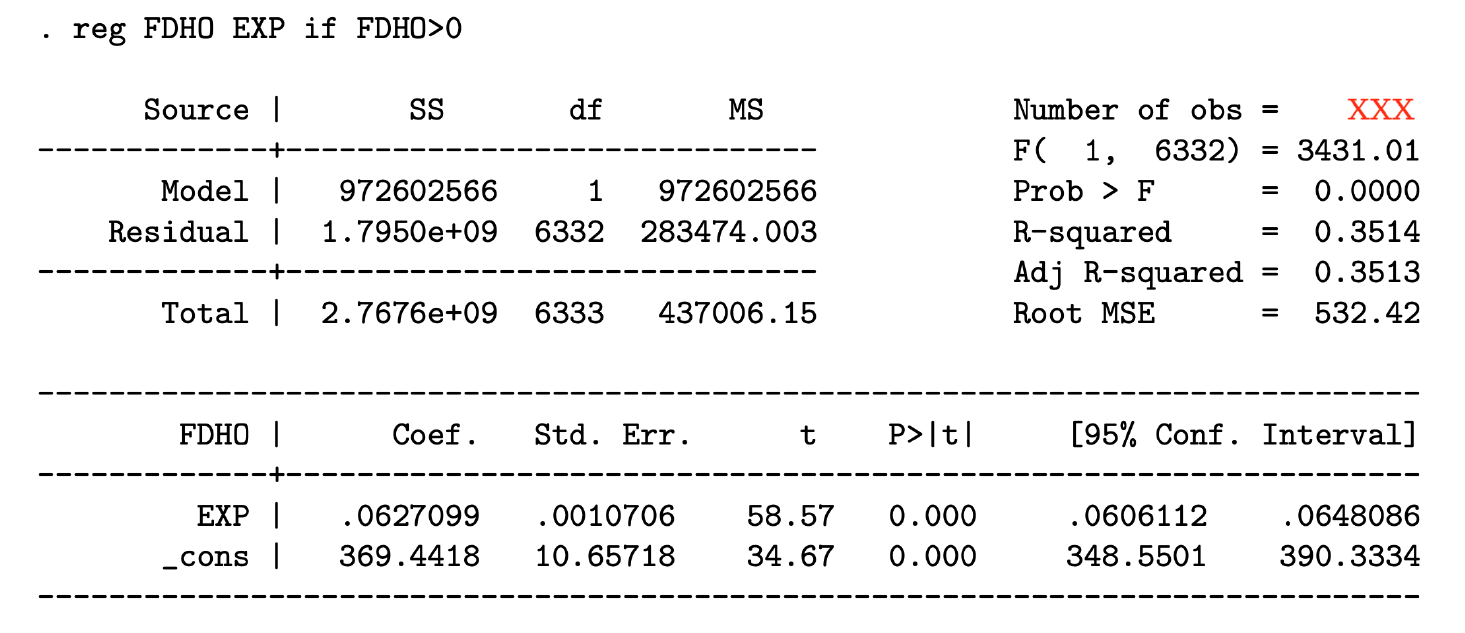
\includegraphics[width=0.85\textwidth]{figures/2021-2022_tests_stata-a.png}
\end{minipage}


Unfortunately, some things are missing. Looking at this output, do the following tasks:

\begin{enumerate}
    \item 
    Give an interpretation of the coefficients estimations.
    
    \item
    Find the number of observations.
    
    \item
    Find the values of TSS, ESS and RSS.
    
    \item
    Explain in your own words what TSS, ESS and RSS are or provide formulas for them.
\end{enumerate}


\item We have a classical linear model 
\[
    Y_i = \beta_1 + \beta_2 X_i + u_i,
\]
where $\beta_1$ and $\beta_2$ are fixed parameters, $u_i$ is a disturbance term that is independently and identically distributed with expected value 0 and population variance $\sigma_u^2$ 
and $i \in \{1, \ldots, n\}$ is the observation index.

Derive the OLS  $\hat \beta_1$ and $\hat \beta_2$ estimators. 
Answers without a solution will not be accepted. You need to provide a full solution.
\end{enumerate}



\subsection{Test 1}

You have 40 minutes to complete the test. Please explain each step of your derivations and state all the assumptions employed. 
Note that different problems can give you different points. Maximum for the test is 10 points.  

\begin{enumerate}
    \item Some practitioners of econometrics consider regressions with transformed variables. 
    For example, if the original model specification is
\[
    Y_i = \beta_1 + \beta_2 X_i + u_i,
\]
the revised specification is
\[
    Y_i^* = \beta_1^* + \beta_2^* X_i^* + v_i,
\]
where
\[
    Y_i^* = \frac{Y_i - a}{c} \text{ and } X_i^* = \frac{X_i - b}{d}.
\]

Knowing that $a, b, c, d$ are some constants and $ c \ne 0, d \ne 0$, express the OLS estimators $\hat\beta_1^*$, $\hat\beta_2^*$ 
in terms of the OLS estimators $\hat\beta_1$, $\hat\beta_2$ [2 points].


\item A novice econometrician estimated a classical linear model 
\[
     Y_i = \beta_1 + \beta_2 X_i + u_i
\]
using 4 observations and obtained the following results:

\begin{tabular}{@{}ccccc@{}}
\toprule
 $Y_i$ & 3 & 7 & 9 & 10\\ 
 $X_i$ & 3 & XXX & XXX & 1\\ 
 $\hat Y_i$ & 4 & 8 & 7 & 11\\ 
\bottomrule
\end{tabular}

Help this econometrician find the estimates of the regression coefficients $\hat \beta_1$ and $\hat \beta_2$ [1 point] and restore the missing values in table [1 point]. 
Can you confirm that these estimations were made using the OLS method? [1 point]

\item 
The output below gives the result of regressing $WAGE$, individual monthly wage measured in thousand rubles, on $TENURE$, total years of work experience a person has.

\begin{minipage}{\textwidth}
    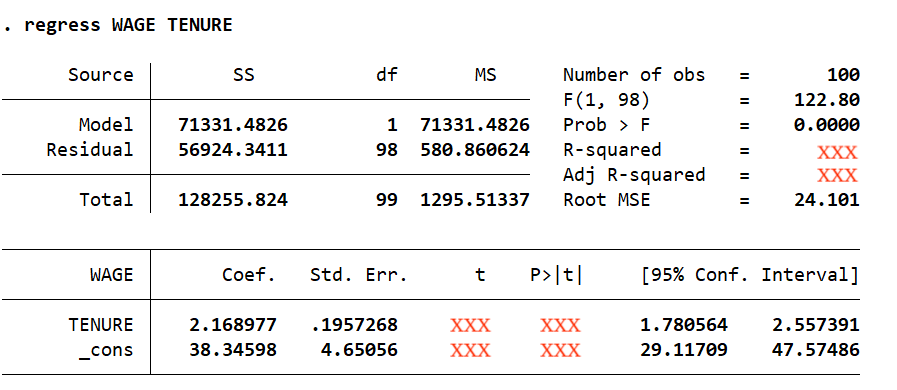
\includegraphics[width=0.85\textwidth]{figures/2021-2022_tests_stata-b.png}
\end{minipage}


Unfortunately, some things are missing. Looking at this output, do the following tasks:

\begin{enumerate}
    \item 
    Give an interpretation of the coefficients estimations [1 point].
    
    \item
    Tell whether coefficients are statistically significant or not (if necessary, you may assume that these hypotheses are tested at a $5\%$ significance level, $t_{crit} \approx 2$) [1 point].
    
    \item
    Find the $R^2$ value [0.5 points].
    
    \item
    Explain in your own words what the $R^2$ value shows [0.5 points].
    
\end{enumerate}

\item We have a linear model 
\[
    Y_i = \beta X_i + u_i,
\]
where $\beta$ is a fixed parameter, $u_i$ is a disturbance term that is independently and identically distributed with expected value 0 and population variance $\sigma_u^2$ 
and $i \in \{1, \ldots, n\}$ is the observation index.


Derive the OLS  $\hat \beta$ estimator. 
Answers without a solution will not be accepted. You need to provide a full solution [2 points].

\end{enumerate}


\subsection{Test 1, answers}

\begin{enumerate}
    \item 
\[
\hat\beta_1^* = \frac{\hat\beta_1 + b \hat\beta_2 -a}{c}, \quad \hat\beta_2^* = \frac{d\hat\beta_2}{c}
\]
\item $\hat\beta_1 = 29/2$, $\hat\beta_2 = -7/2$, $X_2 = 13/7$, $X_3 = 15/7$, 
coefficients were not estimated with OLS as $\sum \hat u_i \neq 0$.
\item 
\begin{enumerate}
    \item A one-year increase in tenure is associated with a 2.2 thousand rubles increase in wage.
    The minimal wage a novice worker (with no experience) gets is 38.5 thousand rubles.
 \item 
 \item $R^2 = 0.556$
 \item $R^2$ is interpreted as the fraction of the sample variation in the response variable that
 is explained by explanatory variables. It shows how well the data fit the regression
 model.

\begin{minipage}{\textwidth}
    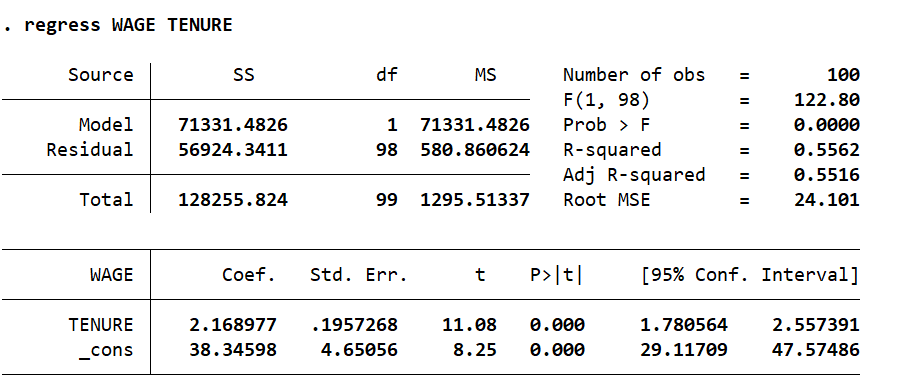
\includegraphics[width=0.85\textwidth]{figures/2021-2022_tests_stata-c.png}
\end{minipage}

\end{enumerate}
\item $\hat\beta = \sum X_i Y_i / \sum X_i^2$
\end{enumerate}

\subsection{Test 2}

You have 40 minutes to complete the test. Please explain each step of your derivations and state
all the assumptions employed. Note that different problems can give you different points.
Maximum for the test is 10 points.


\begin{enumerate}

\item An econometrician estimated this model with $N=55$ observations
\[
\hat{Y}_i = \underset{(0.3)}{3.5} + \underset{(0.4)}{6.1} A_i - \underset{(0.2)}{4.1} B_i. 
\]
Assuming the disturbance term has a standard normal distribution, calculate the 95\%
confidence interval for $\beta_1$ and $\beta_2$ [1 point].
What can you conclude from this calculation [1 point]?


\item An econometrician estimated the model with N observations (persons). In this model: $Earnings$
— hourly earnings of person (\$), $S$ — number of years of study. 
Along with the coefficient estimates, the researcher also got the $R^2$ value.
\[
\widehat{Earnings}_i = \underset{(0.3)}{3.1} + \underset{(?)}{6.1} H_i, R^2= 0.43. 
\]

\begin{enumerate}
    \item Assuming the disturbance term has a standard normal distribution, perform an $F$-test on the
    goodness of fit of the equation writing down the null and alternative hypotheses. What can you
    conclude from this calculation [1 point]?
\item  Give an interpretation of the coefficients estimates [1 point].
\end{enumerate}


\item An econometrician estimated two linear models based on the same 90 observations (persons). In
this model: $Grade$ — the grade a student got for his econometric test (points, out of 10), $H$ — hours
of studying before the test.

Model 1:
\[
\widehat{Grade}_i = \underset{(0.2)}{2.3} + \underset{(0.4)}{3.25} H_i, \quad R^2= 0.43. 
\]
Model 2:
\[
\widehat{Grade}_i = \underset{(0.3)}{4.64} H_i, \quad R^2= 0.52. 
\]
Which model would you use? Explain [2 points].


\item A researcher investigating the determinants of the demand for public transport in a certain city has
the following data for 100 residents for the previous calendar year: expenditure on public transport,
$E$, measured in dollars; number of days worked, $W$; and number of days not worked, $NW$ (by
definition, $NW$ is equal to $365 – W$). He attempts to fit the following model
\[
E_i = \beta_1 + \beta_2 W_i + \beta_3 NW_i + u_i.    
\]

\begin{enumerate}
\item Explain why it is impossible to fit this equation. Give intuitive explanations [1 point].
\item The researcher estimated model using the OLS method. What can we say about the OLS estimator
of coefficients if $u_i$ is a disturbance term that is independently and identically distributed with
expected value $a\neq 0$ [1 point].
\end{enumerate}


\item Prove that the OLS estimator of coefficients in a multiple regression is unbiased 
if the Gauss–Markov conditions are satisfied (use the matrix notation) [1 point].

Derive the variance of the coefficients (use the matrix notation) [1 point].

\end{enumerate}


\subsection{Test 3}
You have 40 minutes to complete the test. Please explain each step of your derivations and state
all the assumptions employed. Note that different problems can give you different points.
Maximum for the test is 10 points.

\begin{enumerate}
\item You are given the following data on 2,000 respondents:
\begin{itemize}
    \item  hourly earnings (Y);
    \item  educational attainment (years) (EDUC);
    \item  total expenditure in year (TE);
    \item  value of the respondent’s house (H);
    \item  mother’s and father’s educational attainment (MEDUC and FEDUC);
    \item  Weight (W);
    \item  Sex (S);
    \item whether the main job was in the government sector or the private (G).
\end{itemize}

As a policy analyst, you are asked to investigate whether there is a difference in estimated impact
of education on earnings for different genders.

Write one equation you can estimate to test this hypothesis. Explain why you chose these
variables, type of model (nonlinear or linear) [1.5 points].

Tell whether a Chow test can be used to test this hypothesis. If not, explain why. If yes, show
how you would perform this test [1 point].

\item An econometrician estimated two models with 100 observations (s.e. in brackets):
\[
\widehat{\ln Y}_i = \underset{(0.2)}{-0.5} + \underset{(0.3)}{3.1} \ln X_i + \underset{(0.1)}{0.4} W_i. 
\]
Assuming the disturbance term has a standard normal distribution, calculate the 95 per cent
confidence intervals for coefficients estimates for $\ln X_i$ and $W_i$. 
Write an interpretation of one of the intervals [1 point].
\[
    \hat{Y}_i = \underset{(0.2)}{-0.5} + \underset{(0.5)}{2.0} X_i + \underset{(3.1)}{2.4} W_i + + \underset{(3.0)}{1.3} D_i + \underset{(1.0)}{2.1} D_i X_i.     
\]
Give interpretation of the coefficients estimates for \textbf{both} models [2 points].

\item An econometrician gained some data from a university and estimated a model based on 300
observations
\[
GPA_i = \beta_1 + \beta_2 Class_i + u_i,
\]
where GPA is the average grade of a student, CLASS is the percentage of attended classes, $u_i$ is a
disturbance term.

The econometrician thinks that talent also must influence the average grade a student gets,
however, this factor is impossible to observe and measure. Thus, the researcher supposes that there
is an endogeneity problem since the effect of talent goes to the disturbance term and talent might
correlate with the percentage of attended classes.

What will happen with the coefficients estimates in case of the endogeneity problem [0.5 points]?

The researcher discovered that the university could provide him with the data on the distance from
a student's house to the university. Explain why this distance factor can be used as an instrumental
variable [1 point].

\item An econometrician estimated the following model with 100 observations:
\[
E_i = \beta_1 + \beta_2 X_i + \beta_3 Z_i + u_i.    
\]

Suspecting that the regression was subject to heteroskedasticity where $\Var(u_i \mid X_i, Z_i) = f(Z_i)$, 
the researcher prepared the following data:


\begin{tabular}{@{}cc@{}}
    \toprule
    $RSS$ from a regression based on the 50 observations with the smallest values of $Z_i$ & $200$ \\ 
    $RSS$ from a regression based on the 50 observations with the largest values of $Z_i$ & $250$ \\
    $R^2$ from auxiliary regression (squared residuals from basic regression — dependent variable 
    and $X_i$, $X^2_i$, $Z_i$, $Z^2_i$, $X_i \cdot Z_i$ — independent variables) & 0.3 \\
    \bottomrule
\end{tabular}
    
\begin{enumerate}
\item Perform the Goldfeld–Quandt test and White test and state your conclusions [2 points].
\item How do you deal with heteroskedasticity? Which methods do you know? Write at least two methods [1 point].
\end{enumerate}

\end{enumerate}

\subsection{Test 4}

You have 40 minutes to complete the test. Please explain each step of your derivations and state all the assumptions employed. 
Note that different problems can give you different points. Maximum for the test is 10 points.  

\begin{enumerate}
    \item A researcher wants to estimate the impact of students' previous achievements on their final grade for the econometrics course. He is planning to estimate the following model:
\[
    Metrics_i = \beta_0 + \beta_1 Maths_i + \beta_2 LinearAlgebra_i + \beta_3 ProbabilityTheory_i + 
    \beta_4 Statistics_i + \epsilon_i
\]
The researcher has the total of $N$ observations ($N$ students who have finished the metrics course). He assumes that:
\begin{itemize}
    \item an extra math point is twice more important than an extra statistics point;
    \item linear algebra knowledge has the same impact as probability theory knowledge.
\end{itemize}

How to test these two statements simultaneously? Which models should be estimated? Write down both models. State the null hypothesis the researcher wants to examine. Show how the F-statistics will look like indicating and explaining the numbers of degrees of freedom. [2 points]

\item The researcher wants to estimate the way person's expenditures on coffee ($COFFEE$) 
depend on his/her income ($INCOME$) and believes that it is necessary to control for a season of the year. 
The season variable ($SEASON$) has the following values: 1 for winter, 2 for spring, 3 for summer and 4 for autumn. 
The researcher assumes that a different linear relationship can correspond to each season.

Write out the equation of the model to be estimated. Indicate the meaning of all variables included in the model. [2 points]

How to test the hypothesis of a uniform (same) linear relationship between income and expenditures for all seasons? 
Carefully write out the main hypothesis, the alternative hypothesis, the formula for calculating the test statistics. [1,5 points]


\item The teacher asked you to find out which factors influence the total number of pages 
of a student's book a person reads during a week's preparation for an exam. 
You want to include the following explanatory variables:

\begin{itemize}
    \item $FREE$ — hours of free time on the week before an exam;
    \item $TRIP$ — duration of the trip from home to university (if the trip is long, a person might use this time for reading);
    \item $GRADES$ — grades for home assignments that a person received before the exam.
\end{itemize}

Your groupmate, who is doing the same task, likes the variables that you have suggested, 
but he decides to include some additional factors and his explanatory variables are:

\begin{itemize}
    \item the same factors that were suggested by you;
    \item $SEX$ — dummy on sex (females are usually more diligent and will spend more time on preparation);
    \item $BURGERS$ — the number of burgers a person has eaten during this week.
\end{itemize}

The teacher says that the first model lacks an important factor ($SEX$), while the second model has an unnecessary factor ($BURGERS$). 
All in all, both students have made some mistakes while specifying their models.
What will be the consequences of each mistake? Which mistake is more dangerous for a researcher and why? [3 points]

\item Choose one paper that was presented during the course (not the one you presented!) and write down its title or authors. 
What is the main research question of the paper? What data do authors use to answer the research question? [1,5 points]

Having studied different aspects of econometric models, 
what can you say about potential problems with the modelling that can arise here? [extra points]
\end{enumerate}


\section{2022-2023}

% !TEX root = ../metrics_hse_exams.tex

\subsection{Контрольная работа 1}

\begin{enumerate}
\item (20 баллов) Была оценена регрессия вида

\[
Y_i = \beta_1 + \beta_2X_{i1} + \beta_3X_{i2} + \beta_4X_{i3} + \beta_5X_{i4} + \varepsilon_i.
\]

Результаты оценивания регрессии представлены в таблице ниже.

\begin{figure}[h]
	\begin{center}
				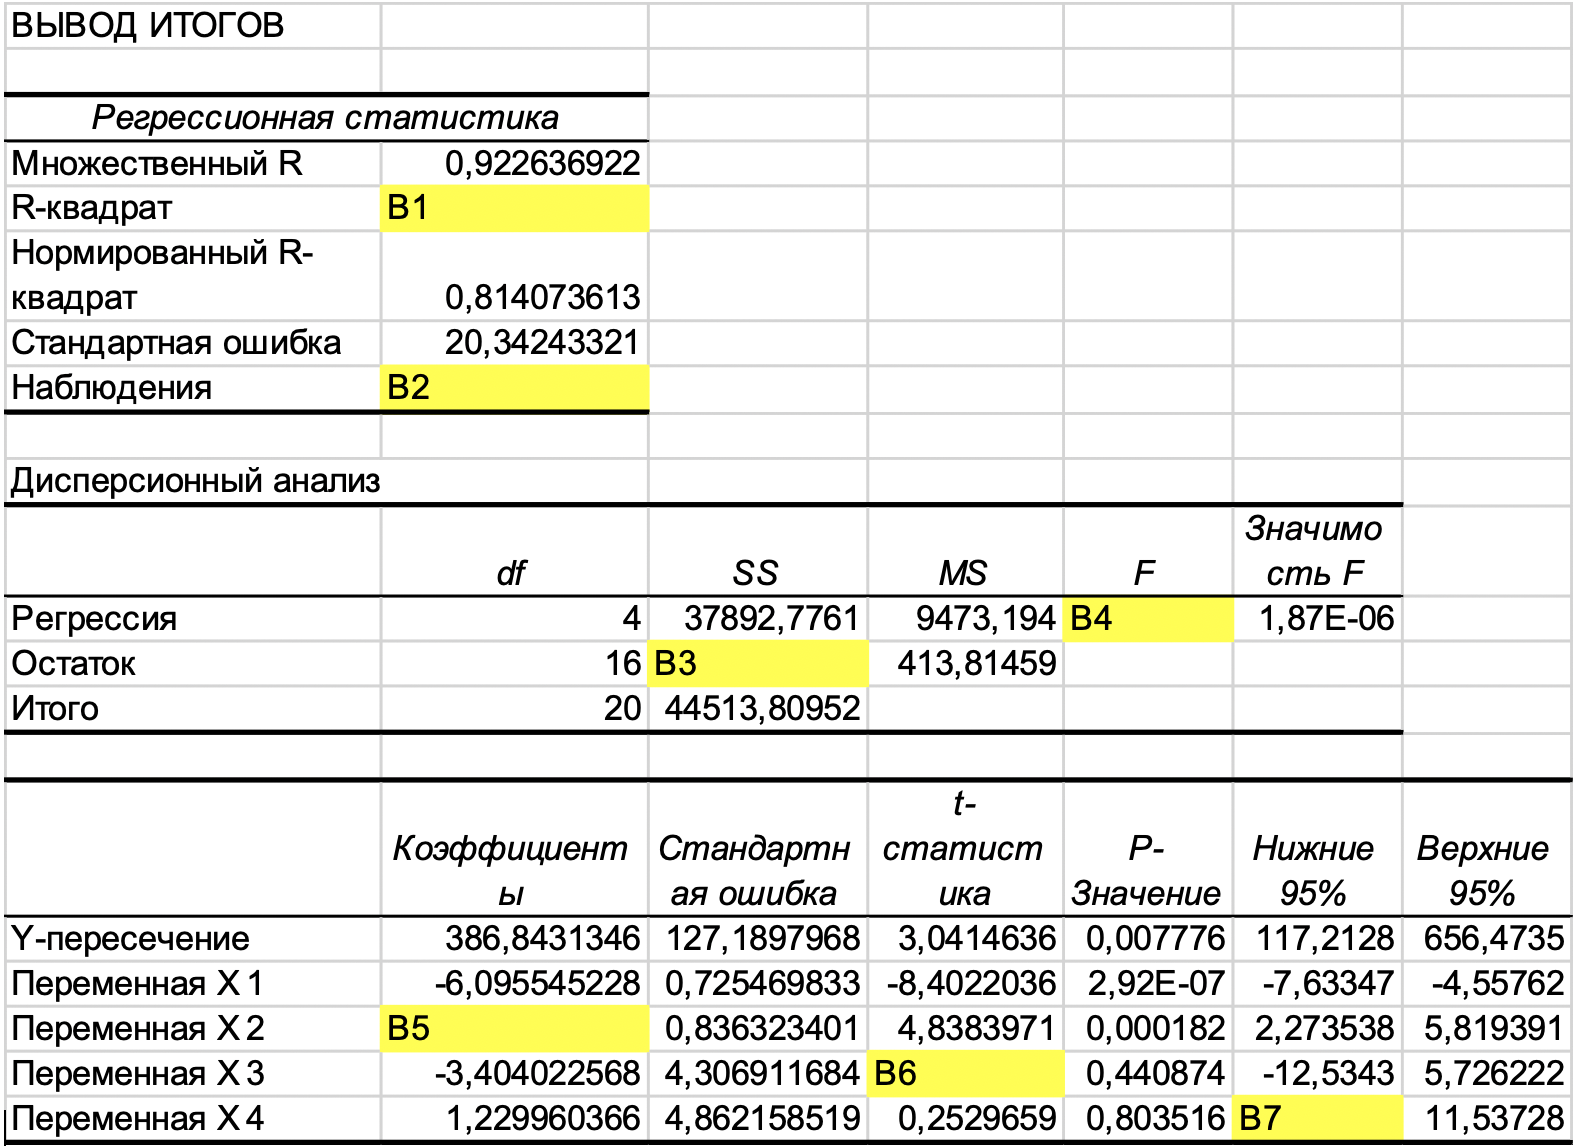
\includegraphics[scale=0.5]{figures/2022-2023_kr1.png}
	\end{center}
\end{figure}

\begin{enumerate}
\item (2 балла) Найдите значение B5.
\item (2 балла) Выпишите оцененное уравнение регрессии.
\item (2 балла) Найдите значение B1.
\item (2 балла) Найдите значение B2.
\item (2 балла) Найдите значение B3.
\item (2 балла) Найдите значение B4.
\item (2 балла) Найдите значение B6.
\item (2 балла) Найдите значение B7.
\item (4 балла) Сделайте вывод о значимости коэффициентов регрессии на уровне значимости 5\% и проинтерпретируйте полученные результаты.
\end{enumerate}

\item (20 баллов) Исследуется зависимость реального дохода на душу населения $y$ (в тыс.долл.) от процента рабочей силы, занятой в сельском хозяйстве, $x_1$ и среднего уровня образования населения в возрасте после 25 лет $x_2$ (число лет, проведенных в учебных заведениях) для 5 развитых стран в 2001 году. По имеющимся данным была оценена следующая модель регрессии:

\[
y_i = \beta_1 + \beta_2x_{i1} + \beta_3x_{i2} + \varepsilon_i.
\]

При этом известно, что

\[
X' X =  \begin{pmatrix}
5 & 3 & 1 \\
3 & 3 & 1 \\
1 & 1 & 1 \\
\end{pmatrix}, \quad (X' X)^{-1} =  \begin{pmatrix}
0.5 & -0.5 & 0 \\
-0.5 & 1 & -0.5 \\
0 & -0.5 & 1.5 \\
\end{pmatrix}, 
\]
\[
X'y =\begin{pmatrix}
15 \\
11 \\
4 
\end{pmatrix}, e'e = 6.5.
\]

\begin{enumerate}
\item (3 балла) Найдите МНК-оценки для параметров модели регрессии.
\item (3 балла) Проинтерпретируйте результаты регрессии.
\item (3 балла) Определите $\widehat{\sigma}^2_{\varepsilon}$, $\widehat{\sigma}^2_{\hb_2}$ и $\widehat{\sigma}^2_{\hb_3}$.
\item (3 балла) Постройте 95\%-ый доверительный интервал для $\beta_2$.
\item (3 балла) Проверьте на 5\%-ом уровне значимости гипотезу о том, что $\beta_2 = 0$ и $\beta_3 = 0$.
\item (2 балла) Спрогнозируйте реальный доход на душу населения для страны, в которой процент рабочей силы, занятой в сельском хозяйстве, составляет 7\% и средний уровень образования населения в возрасте после 25 лет составляет 12 лет.
\item (3 балла) Постройте 95\%-ый доверителный интервал для прогноза из предыдущего пункта.
\end{enumerate}

\item (10 баллов) Рассмотрим следующую регрессионную модель зависимости логарифма заработной платы $\ln (W)$ от уровня образования $Edu$ и опыта работы $Exp$, $Exp^2$:
 
\[
\widehat{\ln (W)_i} = \hb_0 + \hb_1 Edu_i + \hb_2 Exp_i + \hb_3 Exp^2_i.
\]

Модель регрессии была отдельно оценена по выборкам из 20 мужчин и 20 женщин, и
были получены остаточные суммы квадратов $RSS_{male} = 49.4$ и $RSS_{female} = 44.1$ Остаточная сумма квадратов в регрессии, оцененной по объединенной выборке ($RSS_{pooled}$), равна 105.5. Протестируйте на 5\%-ом уровне значимости гипотезу об отсутствии дискриминации в оплате труда между мужчинами и женщинами.

\item (10 баллов) Рассмотрим оценку вида $\tilde\beta = (X'X+rD)^{-1}X'y$ для вектора коэффициентов регрессионного уравнения $y = X\beta + \varepsilon$, где $D$ – диагональная $k \times k$ матрица, состоящая из диагональных элементов матрицы $X'X$.

\begin{enumerate}
\item (5 баллов) Найдите математическое ожидание оценки $\tilde\beta$.
\item (5 баллов) Найдите матрицу ковариаций оценки $\tilde\beta$.
\end{enumerate}
\end{enumerate}



\section{2024-2025}

\subsection{Panda, demo variant «Pumpkin», November 2024}

Midterm will contain 6 problems. 
All the problems have equal weights. 
Midterm duration is 120 minutes. 
No cheatsheet, closed book. 
All topics before (and including) bootstrap may be included. 

\begin{enumerate}
    \item You have estimated the linear regression 
    \[
    \hat y_i  = 3 + 0.2 x_i + 0.5 b_i - 0.7 c_i
    \]
    using big number of observations $n$. 
    Assume all Gauss~— Markov assumptions are satisfied. 

    The estimate of the covariance matrix of coefficients is 
    \[
    \begin{pmatrix}
        2.5 & -0.2 & 0.1  & 0 \\
        ?   &  4.5 & -0.1 & 0.1 \\
        ?   &   ?  & 3.2  & -0.1 \\
        ?   &   ?  &  ?   &  3.5 \\       
    \end{pmatrix}
    \]
    \begin{enumerate}
        \item Construct 95\% confidence interval for $\beta_x$.
        \item Construct 95\% confidence interval for conditional expected value of dependent variable if $x = 1$, $b = -1$, $c = 2$.
        \item Test that $\beta_x + \beta_b = 1$ against $\beta_ x + \beta_b \neq 1$ at 5\% significance level.
    \end{enumerate}


    \item Consider the simple regression model $y_i = \beta_0 + \beta_1 x_i + u_i$.
    Assume that Gauss~— Markov assumptions are satisfied.
    Let $z_i = \sqrt{x}_i$.

    Consider two estimators of $\beta_1$:
    \[
    \hb_1' = \frac{\sum_{i=1}^n(z_i - \bar z)y_i}{\sum_{i=1}^n(z_i - \bar z)x_i}, \quad \hb_1'' = \frac{\sum_{i=1}^n(z_i - \bar z)y_i}{\sum_{i=1}^n(z_i - \bar z)z_i}.
    \]
    \begin{enumerate}
        \item Calculate $\E(\hb_1' \mid x)$ and $\E(\hb_1'' \mid x)$. Are estimators unbiased conditionally on $x$?
        \item Are estimators $\hb_1'$ and $\hb_1''$ consistent?
    \end{enumerate}


    \item You have $300$ observations in total and you estimated the regression 
    \[
    \hat y_i = \hb_0 + \hb_1 x_i + \hb_2 v_i + \hb_3 w_i
    \]
    using different parts of your dataset.

    \begin{tabular}{rr}
        \toprule
        Observations & Result \\
        \midrule
        $1, \dots, 300$ & $\SSR = 300$, $\SST = 500$ \\
        $1, \dots, 200$ & $\SSR = 150$ \\
        $201, \dots, 300$ & $\SSR = 100$ \\
        \bottomrule
    \end{tabular}


    Assume for each case that Gauss~— Markov assumptions for the unrestricted model are satisfied. 
    Use 5\% critical level. 
    % Alternative hypothesis in each case is the violation of at least on constraint in $H_0$.

    \begin{enumerate}
        \item Test that $\beta_1 = \beta_2 = \beta_3 = 0$ for the whole dataset against alternative that at least one of the coefficients is non-zero.
        \item Test for the absence of a structural break between part one (observations $1$, \dots, $200$) and part two (observations $201$, \dots, $300$) of your dataset.
        Here in $H_0$ you assume that the relation $y_i = \beta_0 + \beta_1 x_i + \beta_2 v_i + \beta_3 w_i + u_i$
        holds for the whole dataset. 
        And in $H_1$ you assume that different linear models may be valid for the two parts of your dataset.
        \item Consider again $H_0$ that the relation $y_i = \beta_0 + \beta_1 x_i + \beta_2 v_i + \beta_3 w_i + u_i$
        holds for the whole dataset.
        But now in $H_1$ assume that the linear relation $y_i = \beta_0 + \beta_1 x_i + \beta_2 v_i + \beta_3 w_i + u_i$
        holds only for the first part of the dataset. 
        You do not assume linear relation between $y_i$ and predictors in the second part.
        Test $H_0$ against $H_1$.
    \end{enumerate}

    \item Consider three observations: $x = (1, 1, 0)$ and $y = (1, 3, 5)$.
    \begin{enumerate}
        \item Estimate $\hb_0$ and $\hb_1$ in the regression $\hat y_i = \hb_0 + \hb_1 x_i$ using OLS.
        \item Calculate sum of squared residuals, sum of squared explained, total sum squares and $R^2$.
        \item Under Gauss~— Markov assumptions estimate the variance of random error term.
        \item Under Gauss~— Markov assumptions estimate the variance matrix of $\hb$ vector. 
    \end{enumerate}

    \item Consider the model $y = X\beta + u$ where $\beta$ is non-random,
    $\E(u \mid X ) = 0$, the matrix $X$ of size $n\times k$ has $\rank X = k$, 
    but $\Var(u \mid X) = \sigma^2 W$ with $W \neq I$.
    Let $\hb$ be the standard OLS estimator of $\beta$.

    \begin{enumerate}
        \item Find $\E(\hb \mid X)$, $\E(\hb)$.
        \item Find $\Var(\hb \mid X)$.
        \item How do you think, will the standard confidence interval for $\beta$ be valid in this case?
        \item Find $\Cov(y, \hb \mid X)$.
    \end{enumerate}

    \item Consider two multivariate regressions estimated by OLS.
    Regression $A$: 
    \[
    \hat y = X_1 \hb_1 + X_2 \hb_2.
    \]
    
    The matrices $X_1$ and $X_2$ are two blocks of regressors, 
    the matrix $X_1$ has size $n\times k_1$, 
    the matrix $X_2$ has size $n\times k_2$.
    Let $X = \begin{pmatrix}
        X_1 X_2
    \end{pmatrix}$ be the full regressors matrix. 

    Consider projection matrix $H_1$ that projects vectors on the span of columns of $X_1$.
    Let $M_1 = I - H_1$ where $I$ is an identity matrix, $y' = M_1 y$, $X_2' = M_1 X_2$.
    Regression $B$:
    \[
    \hat y' = X_2' \hat{\gamma}.
    \]

    \begin{enumerate}
        \item Are estimators $\hb_2$ and $\hat \gamma$ equal?
        \item Are residuals in both regressions equal?
    \end{enumerate}

\end{enumerate}

\subsection{Panda, demo variant «Bat», November 2024}
\begin{enumerate}
    \item % комбинаторика
    Foma estimated simple regression model using three observations and calculated the forecasts $\hat{y}_i$. 
    Unfortunately he remembers only this table:

    \begin{tabular}{rr}
    \toprule
    $y_i$ & $\hy_i$ \\
    \midrule
    $0$ & $1$ \\
    $6$ & ? \\
    $6$ & ? \\
    \bottomrule
    \end{tabular}
    
    He recalls that $\hat y_3 > \hat y_2$. 
    
    Help Foma to reconstruct the missing entries in the table. 
    
    \item Consider the partially hidden output from the Stata package:
    
    \begin{minipage}{\textwidth}
        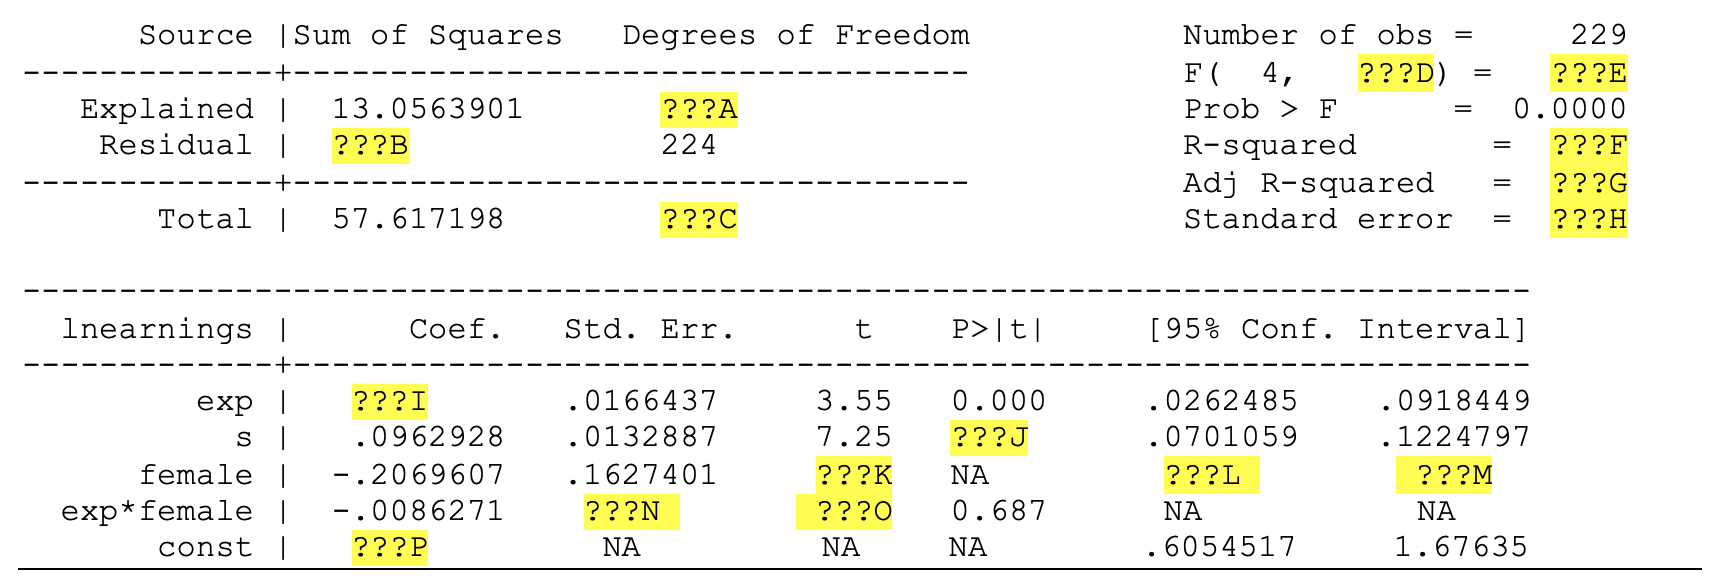
\includegraphics[scale=0.6]{figures/partial_stata_table.png}
    \end{minipage}

    That's the standard regression table reported by all software packages. 
    Here the letters $A$, $B$, \dots{ } just play the role of identifiers. 
    
    Reconstruct all the yellow entries with question marks. 
    

    \item Scared of proofs? That's Halloween, you should be scared!
    \begin{enumerate}
        \item Prove that in the simple regression $\hat y_i = \hb_0 + \hb_1 x_i$ the 
        standard $t$-statistic $t$ for the test $H_0$: $\beta_1 = 0$ and 
        the standard $F$-statistic $F$ for the same test satisfy the relation $t^2 = F$.
        \item Prove that in the simple regressions $\hat y_i = \hb_0 + \hb_1 x_i$ and 
        $\hat x_i = \hat{\gamma}_0 + \hat{\gamma}_1 y_i$ the determination coefficients are equal. 
    \end{enumerate}


    \item Consider the model $y = X\beta + u$ on the training set where $\beta$ is non-random,
    $\E(u \mid X) = 0$, the matrix $X$ of size $n\times k$ has $\rank X = k$, 
    but $\Var(u \mid X) = \sigma^2 I$, where $I$ is an identity matrix. 
    Observations are independent. 
    Let $\hb$ be the standard OLS estimator of $\beta$ using the training set data. 
    You have a test set with the same type of dependency $y' = X' \beta + u'$,
    $\E(u' \mid X') = 0$, $\Var(u' \mid X') = \sigma^2 I$.
    You make the forecast $\hat y'$ for the test set, $\hat y' = X' \hat\beta$.

    \begin{enumerate}
        \item Find $\E(\hat y' \mid X, X')$.
        \item Find $\Var(y' - \hat y' \mid X, X')$.
        \item Find $\Cov(\hb, y' - \hat y' \mid X, X')$.
    \end{enumerate}

    \item Let $u = (u_1, u_2, u_3)$ be the vector of iid standard normal random variables. 
    Denote the linear span of the vector $(1, 1, 0)$ be $V$.
    Let $W = V^{\perp}$ be the orthogonal complement of $V$ in $\RR^3$. 

    \begin{enumerate}
        \item Find $\dim V$, $\dim W$.
        \item Find the projection matrix $H$ that projects vectors from $\RR^3$ onto $V$.
    \end{enumerate}
    Let $v = Hu$ and $w = (I - H)u$.
    \begin{enumerate}[resume]
        \item Find the law of distribution of the random variables $v^T v$ and $\norm{w}^2$.
        \item Find the distribution of $2v^Tv/(w^Tw)$.
    \end{enumerate}

    \item Assume that the true model is $y_i = \beta_0 +  u_i$ and $u_i$ are iid normally distributed with zero mean and variance $\sigma^2$.
    There are $n$ observations.
    We estimate regression $\hat y_i = \hat \beta_0 + \hat\beta_1 x_i$ using OLS.

    \begin{enumerate}
        \item Find $\E(\hat \beta_1 \mid x)$  and $\E(\hat\beta_1)$.
        \item Find $\E(R^2)$.
        \item Find $\E(R^2_{adj})$ for the adjusted coefficient 
        \[
            R^2_{adj} = 1 - \frac{\SSR / (n - 2)}{\SST / (n - 1)}.
        \]
        
    \end{enumerate}

\end{enumerate}

\end{document}

%Из определения условного ожидания, $\E(X \mid A) = \E(X \cdot I_A) / \P(A)$, 
%легко получаются определения условной дисперсии, $\Var(X \mid A) = \E(X^2 \mid A) - (\E(X \mid A))^2$,
%условной ковариации $\Cov(X, Y \mid A) = \E(XY \mid A) - \E(X \mid A) \E(Y \mid A)$ и даже корреляции, 
%$\Corr(X, Y \mid A) = \Cov(X, Y \mid A) / \sqrt{\Var(X \mid A)\Var(Y \mid A)}$.

% здесь проектируемая часть



\end{document}



\end{document}
